\documentclass[aspectratio=169]{beamer}
\IfFileExists{beamerthememetropolis.sty}{\usetheme{metropolis}}{\usetheme{default}}
\usepackage[utf8]{inputenc}
\usepackage[T1]{fontenc}
\usepackage{booktabs}
\usepackage{graphicx}
\usepackage{amsmath}
\usepackage{xcolor}
\usepackage{tikz}
\definecolor{shipblue}{RGB}{20,74,130}
\definecolor{warningorange}{RGB}{210,105,30}
\setbeamercolor{structure}{fg=shipblue}
\setbeamercolor{alerted text}{fg=warningorange}
\setbeamertemplate{navigation symbols}{}
\title{EXEC\_12: EndTop photon budget --- pedagogical review}
\subtitle{t_N distributions, Fano/Landau motivation, window-track mechanism, full scan}
\author{Rene Rios (ULS)}
\date{June 11, 2026}
\begin{document}
\begin{frame}{Configuration and provenance}

\begin{columns}[T]\column{0.62\textwidth}
\textbf{Branch:} \texttt{feat/endtop-sslg4}\\
\textbf{Commits:} \texttt{0201413}, \texttt{7b4bc80}, \texttt{ad26d78},
\texttt{bcefa24}, \texttt{bdfe955}; this deck is generated from those published sources
\begin{itemize}\small
  \item 31 positions $\times$ 2000 events; 16 End + 70 Top channels; jitter fixed to zero.
  \item EJ-204 via SSLG4 \texttt{OPSC-101}: yield 10400/MeV, $\tau_r=0.7$ ns,
        $\tau_d=1.8$ ns, ABSLENGTH=160 cm (verified effective MPT inputs).
  \item Broadcom AFBR-S4N66P024M: PDE 63\% at 420 nm.
\end{itemize}
\column{0.35\textwidth}
\begin{alertblock}{Scope}
Top 70 SiPM is a simulation coverage study. Real hardware: 32 Top SiPMs.
All reported timing is intrinsic, without SPTR or electronics jitter.
\end{alertblock}
\end{columns}

\end{frame}
\begin{frame}{EndTop geometry and channel map}

\begin{columns}[T]\column{0.55\textwidth}
\begin{itemize}
 \item EJ-204 bar: $1400\times60\times10$ mm$^3$.
 \item End L IDs 0--7; End R IDs 8--15.
 \item Top L IDs 16--50: $-692,-672,\ldots,-12$ mm.
 \item Top R IDs 51--85: $+12,+32,\ldots,+692$ mm.
 \item Each Top element and window: $6\times6$ mm$^2$.
\end{itemize}
\column{0.42\textwidth}
\begin{block}{Exact constraints}
First centers are 5 mm from each bar end. Pitch is 20 mm except the deliberate
central $-12/+12$ mm pair, whose pitch is 24 mm.
\end{block}
\end{columns}

\end{frame}
\begin{frame}{Instrumented and wrapped faces}

\centering\begin{tabular}{lll}\toprule
Face & Optical state & Readout \\ \midrule
$-X$, $+X$ & open & 8 End SiPMs each \\
$+Y$ & Mylar with 70 exact windows & 70 Top SiPMs \\
$-Y$, $-Z$, $+Z$ & complete Mylar & none \\
\bottomrule\end{tabular}
\vspace{0.5cm}
\begin{block}{External layer}
Black Tedlar is deliberately not modeled; it only blocks ambient light.
The non-reflected Mylar fraction is already absorbed in the optical model.
\end{block}

\end{frame}
\begin{frame}{Window optics: why timing and collection change}

\centering
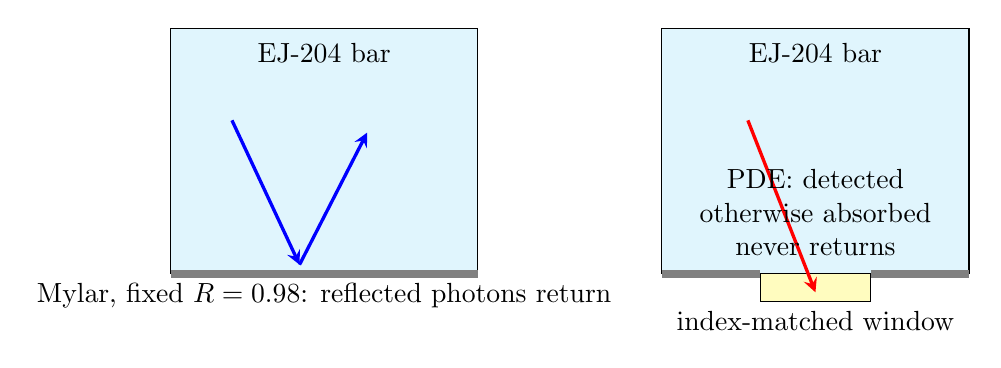
\begin{tikzpicture}[scale=0.78,>=stealth]
 \draw[fill=cyan!12] (0,0) rectangle (5,4);
 \node at (2.5,3.6) {EJ-204 bar};
 \draw[line width=3pt,gray] (0,0) -- (5,0);
 \node[below] at (2.5,0) {Mylar, fixed $R=0.98$: reflected photons return};
 \draw[->,very thick,blue] (1.0,2.5) -- (2.1,0.15);
 \draw[->,very thick,blue] (2.1,0.15) -- (3.2,2.3);
 \draw[fill=cyan!12] (8,0) rectangle (13,4);
 \node at (10.5,3.6) {EJ-204 bar};
 \draw[line width=3pt,gray] (8,0) -- (9.6,0);
 \draw[line width=3pt,gray] (11.4,0) -- (13,0);
 \draw[fill=yellow!25] (9.6,-0.45) rectangle (11.4,0);
 \node[below] at (10.5,-0.45) {index-matched window};
 \draw[->,very thick,red] (9.4,2.5) -- (10.5,-0.3);
 \node[align=center] at (10.5,1.0) {PDE: detected\\otherwise absorbed\\never returns};
\end{tikzpicture}
\begin{alertblock}{Consequence}
Every window is an optical drain. Long, multiply reflected paths have more chances
to meet one, so late End photons are preferentially removed.
\end{alertblock}

\end{frame}
\section{Key positions}
\begin{frame}{Position x=-690 mm}

\begin{columns}[T]
  \column{0.52\textwidth}
  
\includegraphics[width=\textwidth]{figs/muon_-690mm_geometry.png}
  \column{0.46\textwidth}
  
\includegraphics[width=\textwidth]{figs/muon_-690mm_top_profile.png}
  \tiny
  \begin{tabular}{lr}
    \toprule Quantity & Value \\ \midrule
    End L $N_{pe}$ & $3363.1\pm18.1$ \\
    End R $N_{pe}$ & $41.1\pm0.3$ \\
    Nearest Top ID & 16 (window-track exception) \\
    Nearest Top $N_{pe}$ & $350.9\pm2.0$ \\
    Nearest Top $\langle t\rangle$ &
      $2.7863\pm0.0023$ ns \\
    Nearest Top FPT & $0.34278\pm0.00023$ ns \\
    \bottomrule
  \end{tabular}
\end{columns}

\end{frame}
\begin{frame}{Run 1 $|$ x = -690 mm $|$ Photon arrival $\langle N(t)\rangle$}
\centering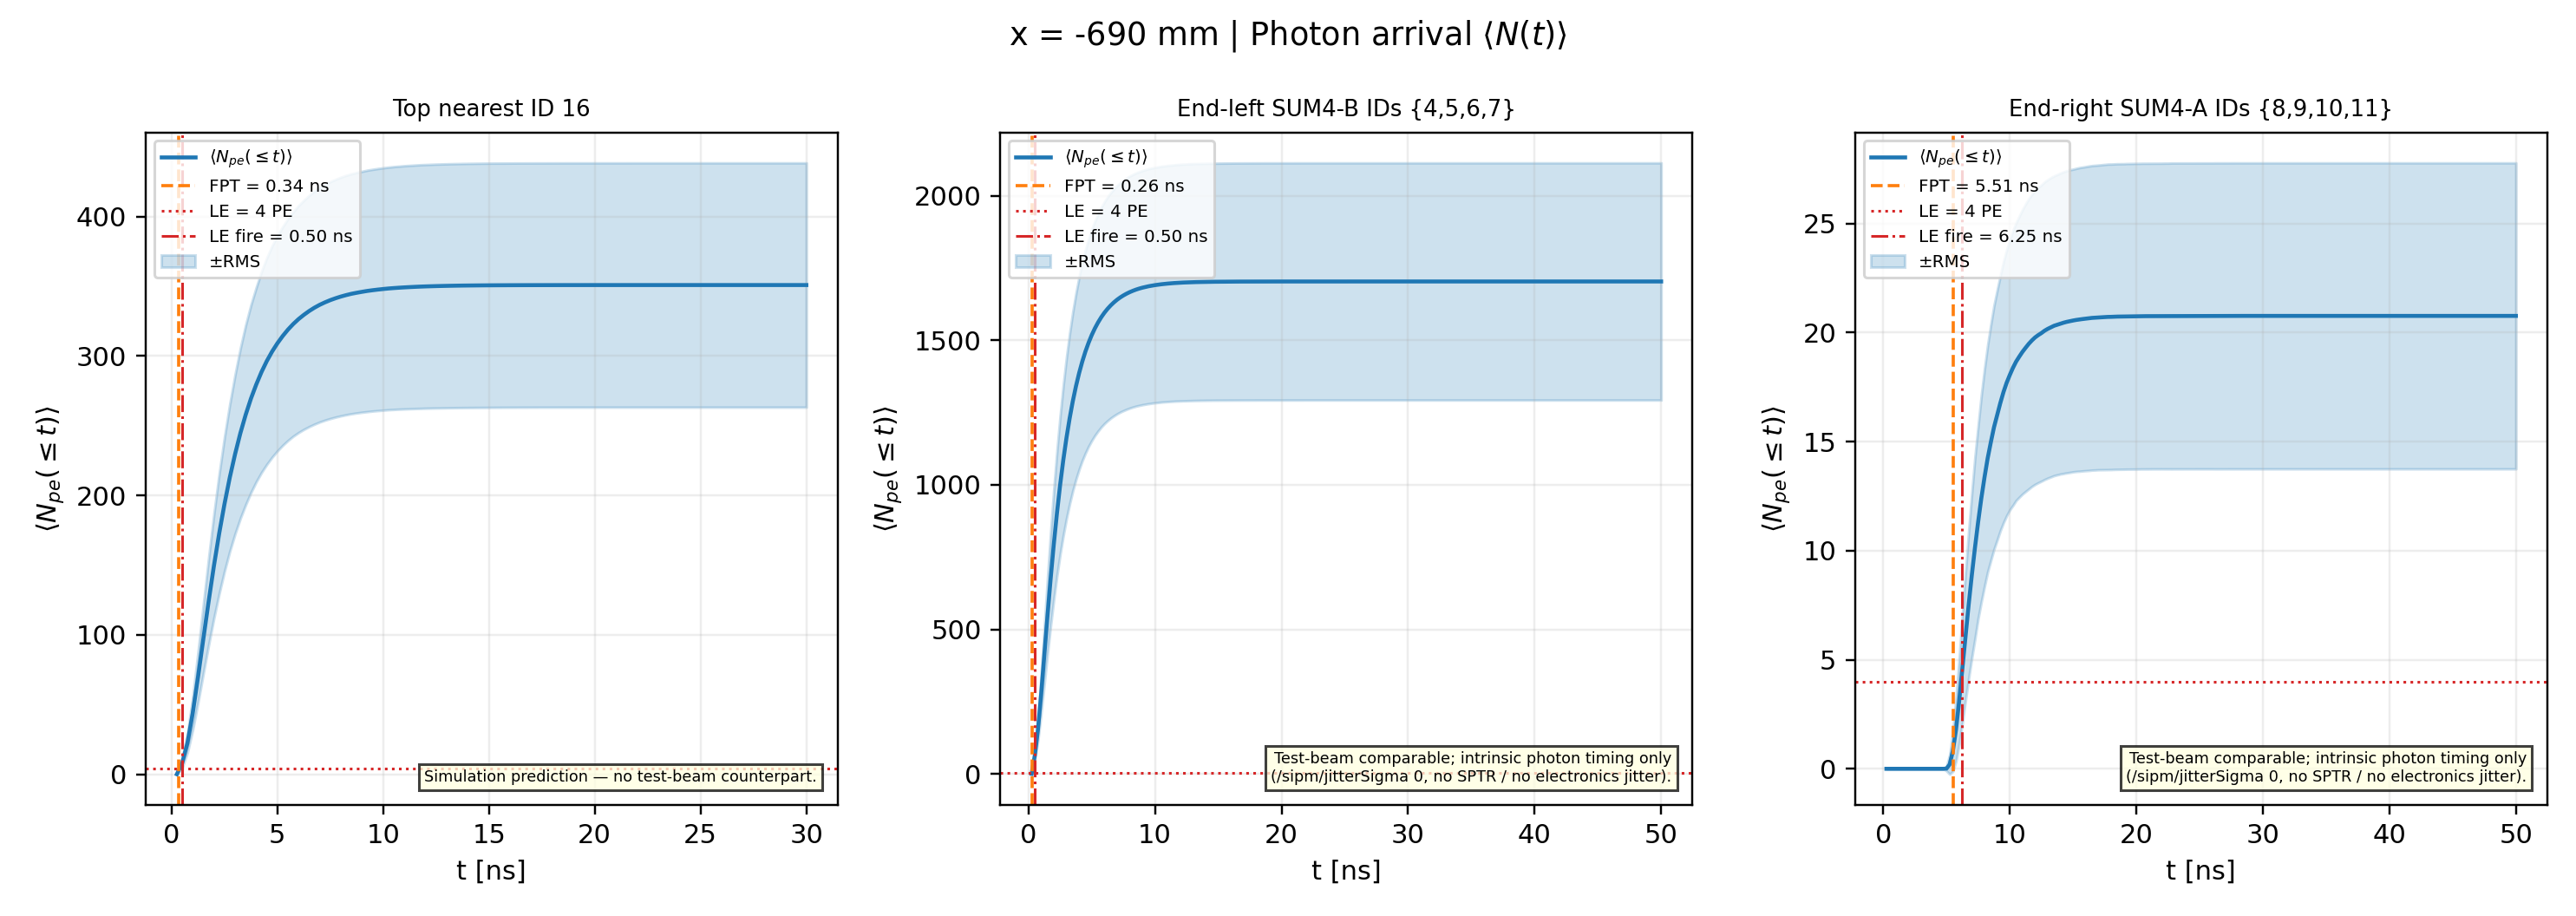
\includegraphics[width=\textwidth,height=0.78\textheight,keepaspectratio]{figs/exec11_arrival_-690mm.png}
\end{frame}
\begin{frame}{Run 1 $|$ x = -690 mm $|$ Time-to-threshold $t_N$}
\centering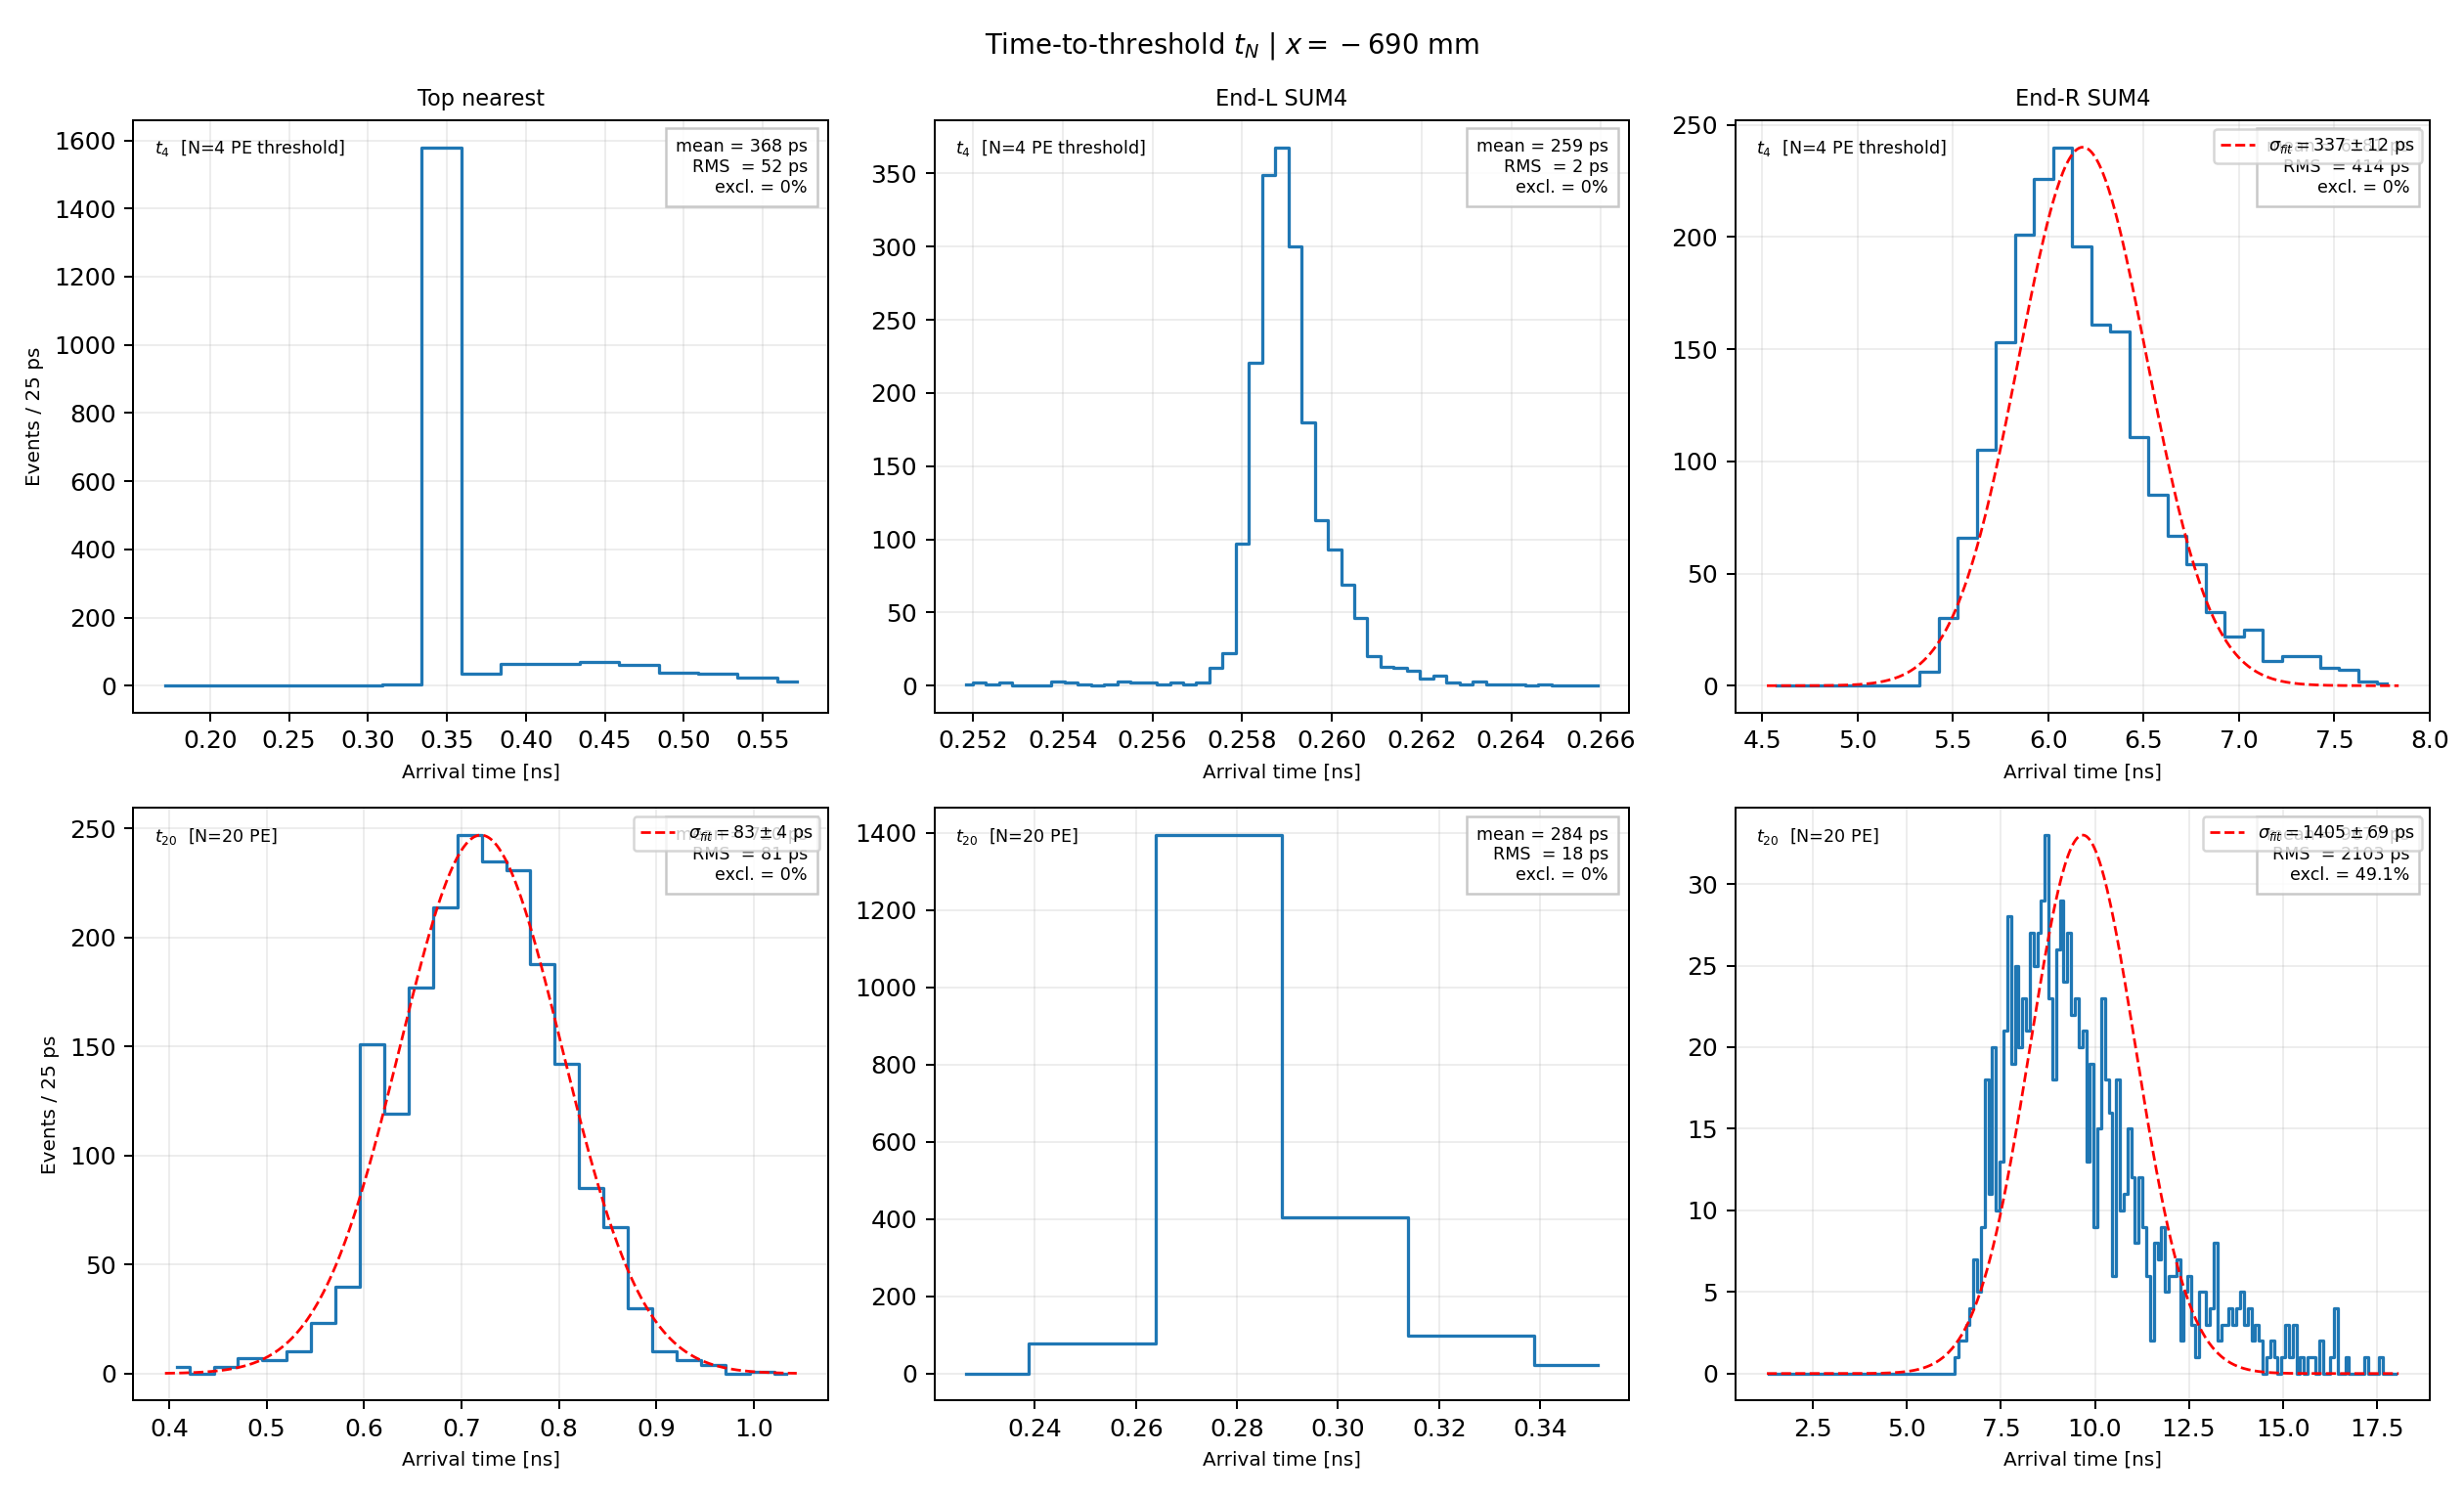
\includegraphics[width=\textwidth,height=0.84\textheight,keepaspectratio]{figs/exec12_tN_-690mm.png}
\end{frame}
\begin{frame}{Position x=-650 mm}

\begin{columns}[T]
  \column{0.52\textwidth}
  
\includegraphics[width=\textwidth]{figs/muon_-650mm_geometry.png}
  \column{0.46\textwidth}
  
\includegraphics[width=\textwidth]{figs/muon_-650mm_top_profile.png}
  \tiny
  \begin{tabular}{lr}
    \toprule Quantity & Value \\ \midrule
    End L $N_{pe}$ & $2366.2\pm13.1$ \\
    End R $N_{pe}$ & $44.3\pm0.3$ \\
    Nearest Top ID & 18 (window-track exception) \\
    Nearest Top $N_{pe}$ & $351.0\pm2.0$ \\
    Nearest Top $\langle t\rangle$ &
      $2.7779\pm0.0023$ ns \\
    Nearest Top FPT & $0.34270\pm0.00024$ ns \\
    \bottomrule
  \end{tabular}
\end{columns}

\end{frame}
\begin{frame}{Run 2 $|$ x = -650 mm $|$ Photon arrival $\langle N(t)\rangle$}
\centering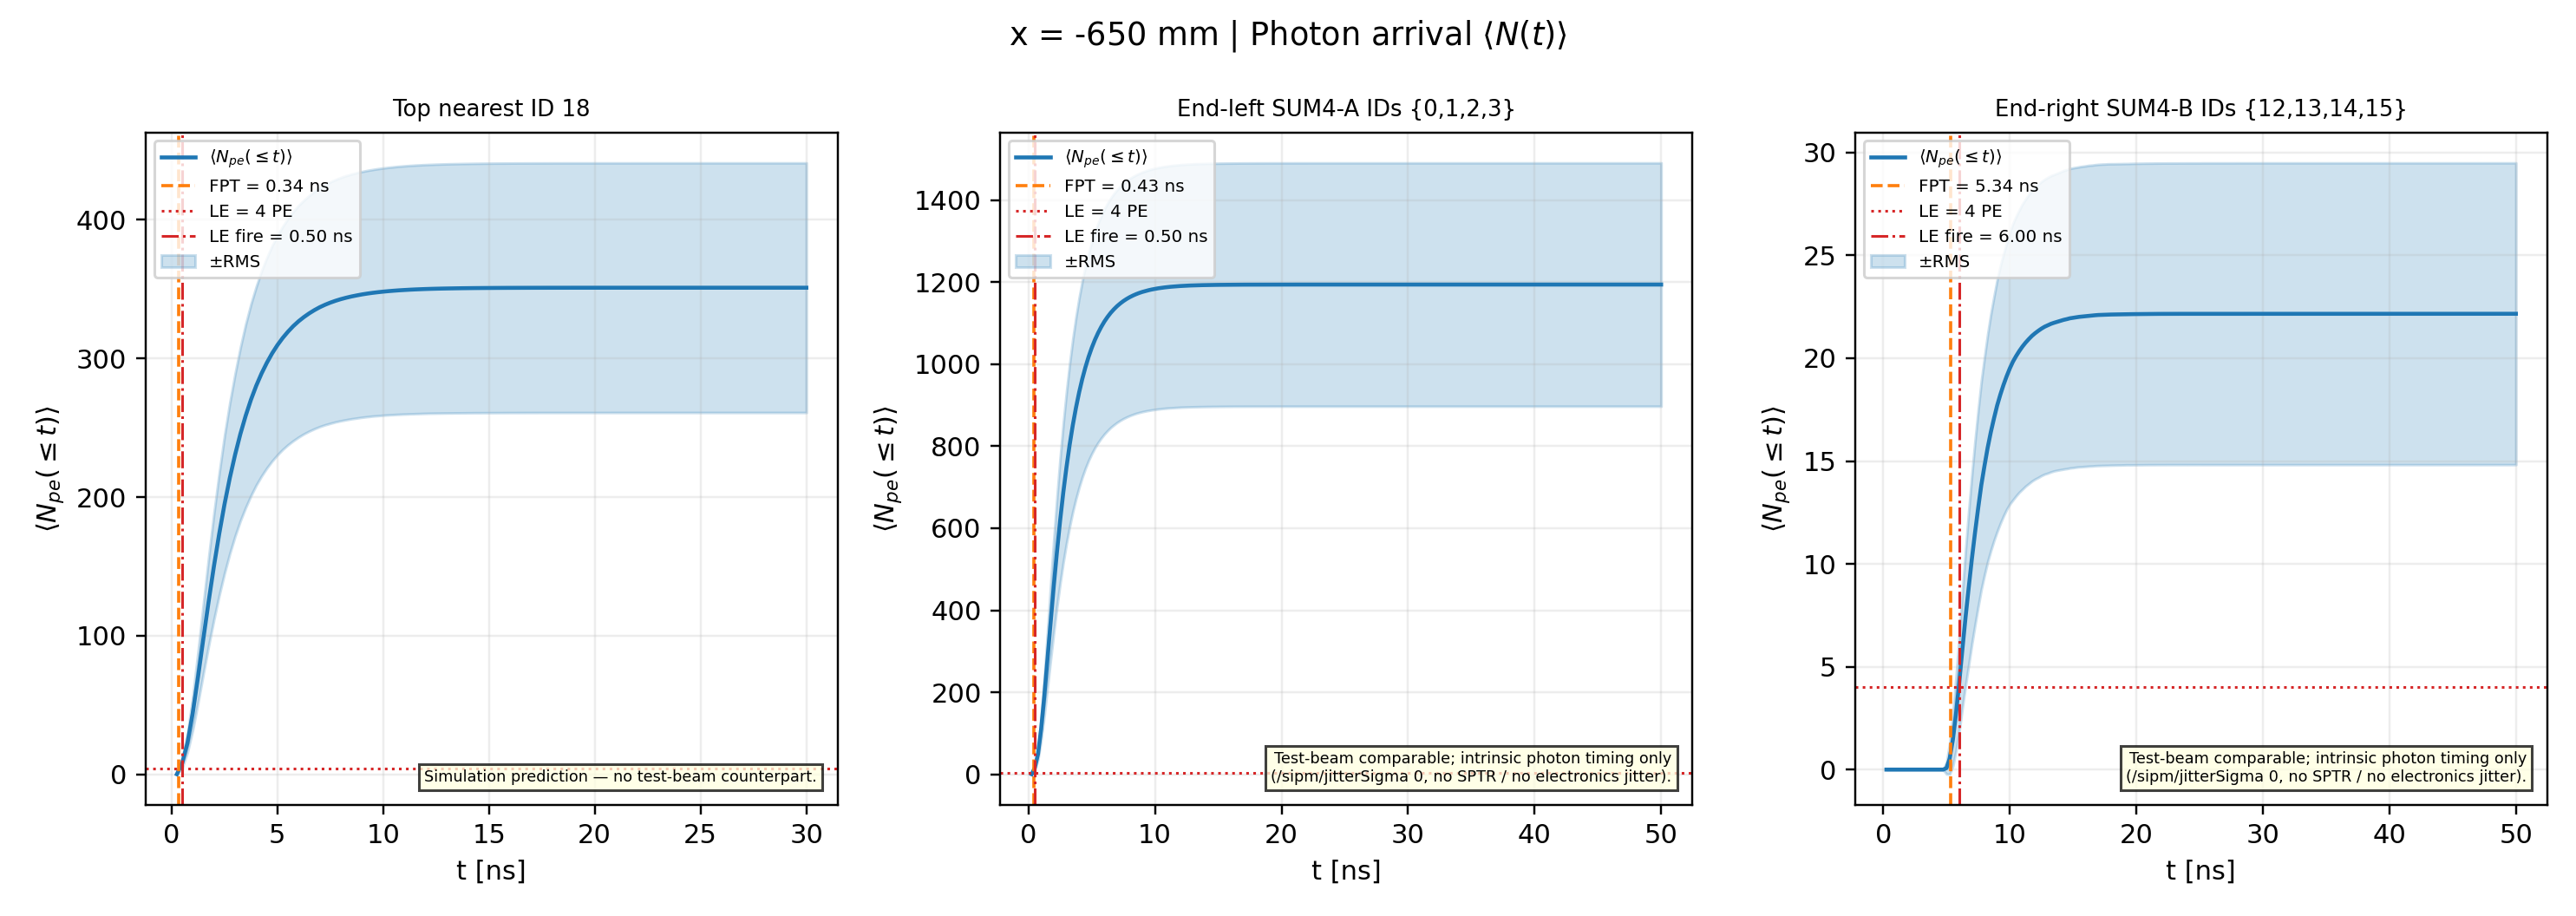
\includegraphics[width=\textwidth,height=0.78\textheight,keepaspectratio]{figs/exec11_arrival_-650mm.png}
\end{frame}
\begin{frame}{Run 2 $|$ x = -650 mm $|$ Time-to-threshold $t_N$}
\centering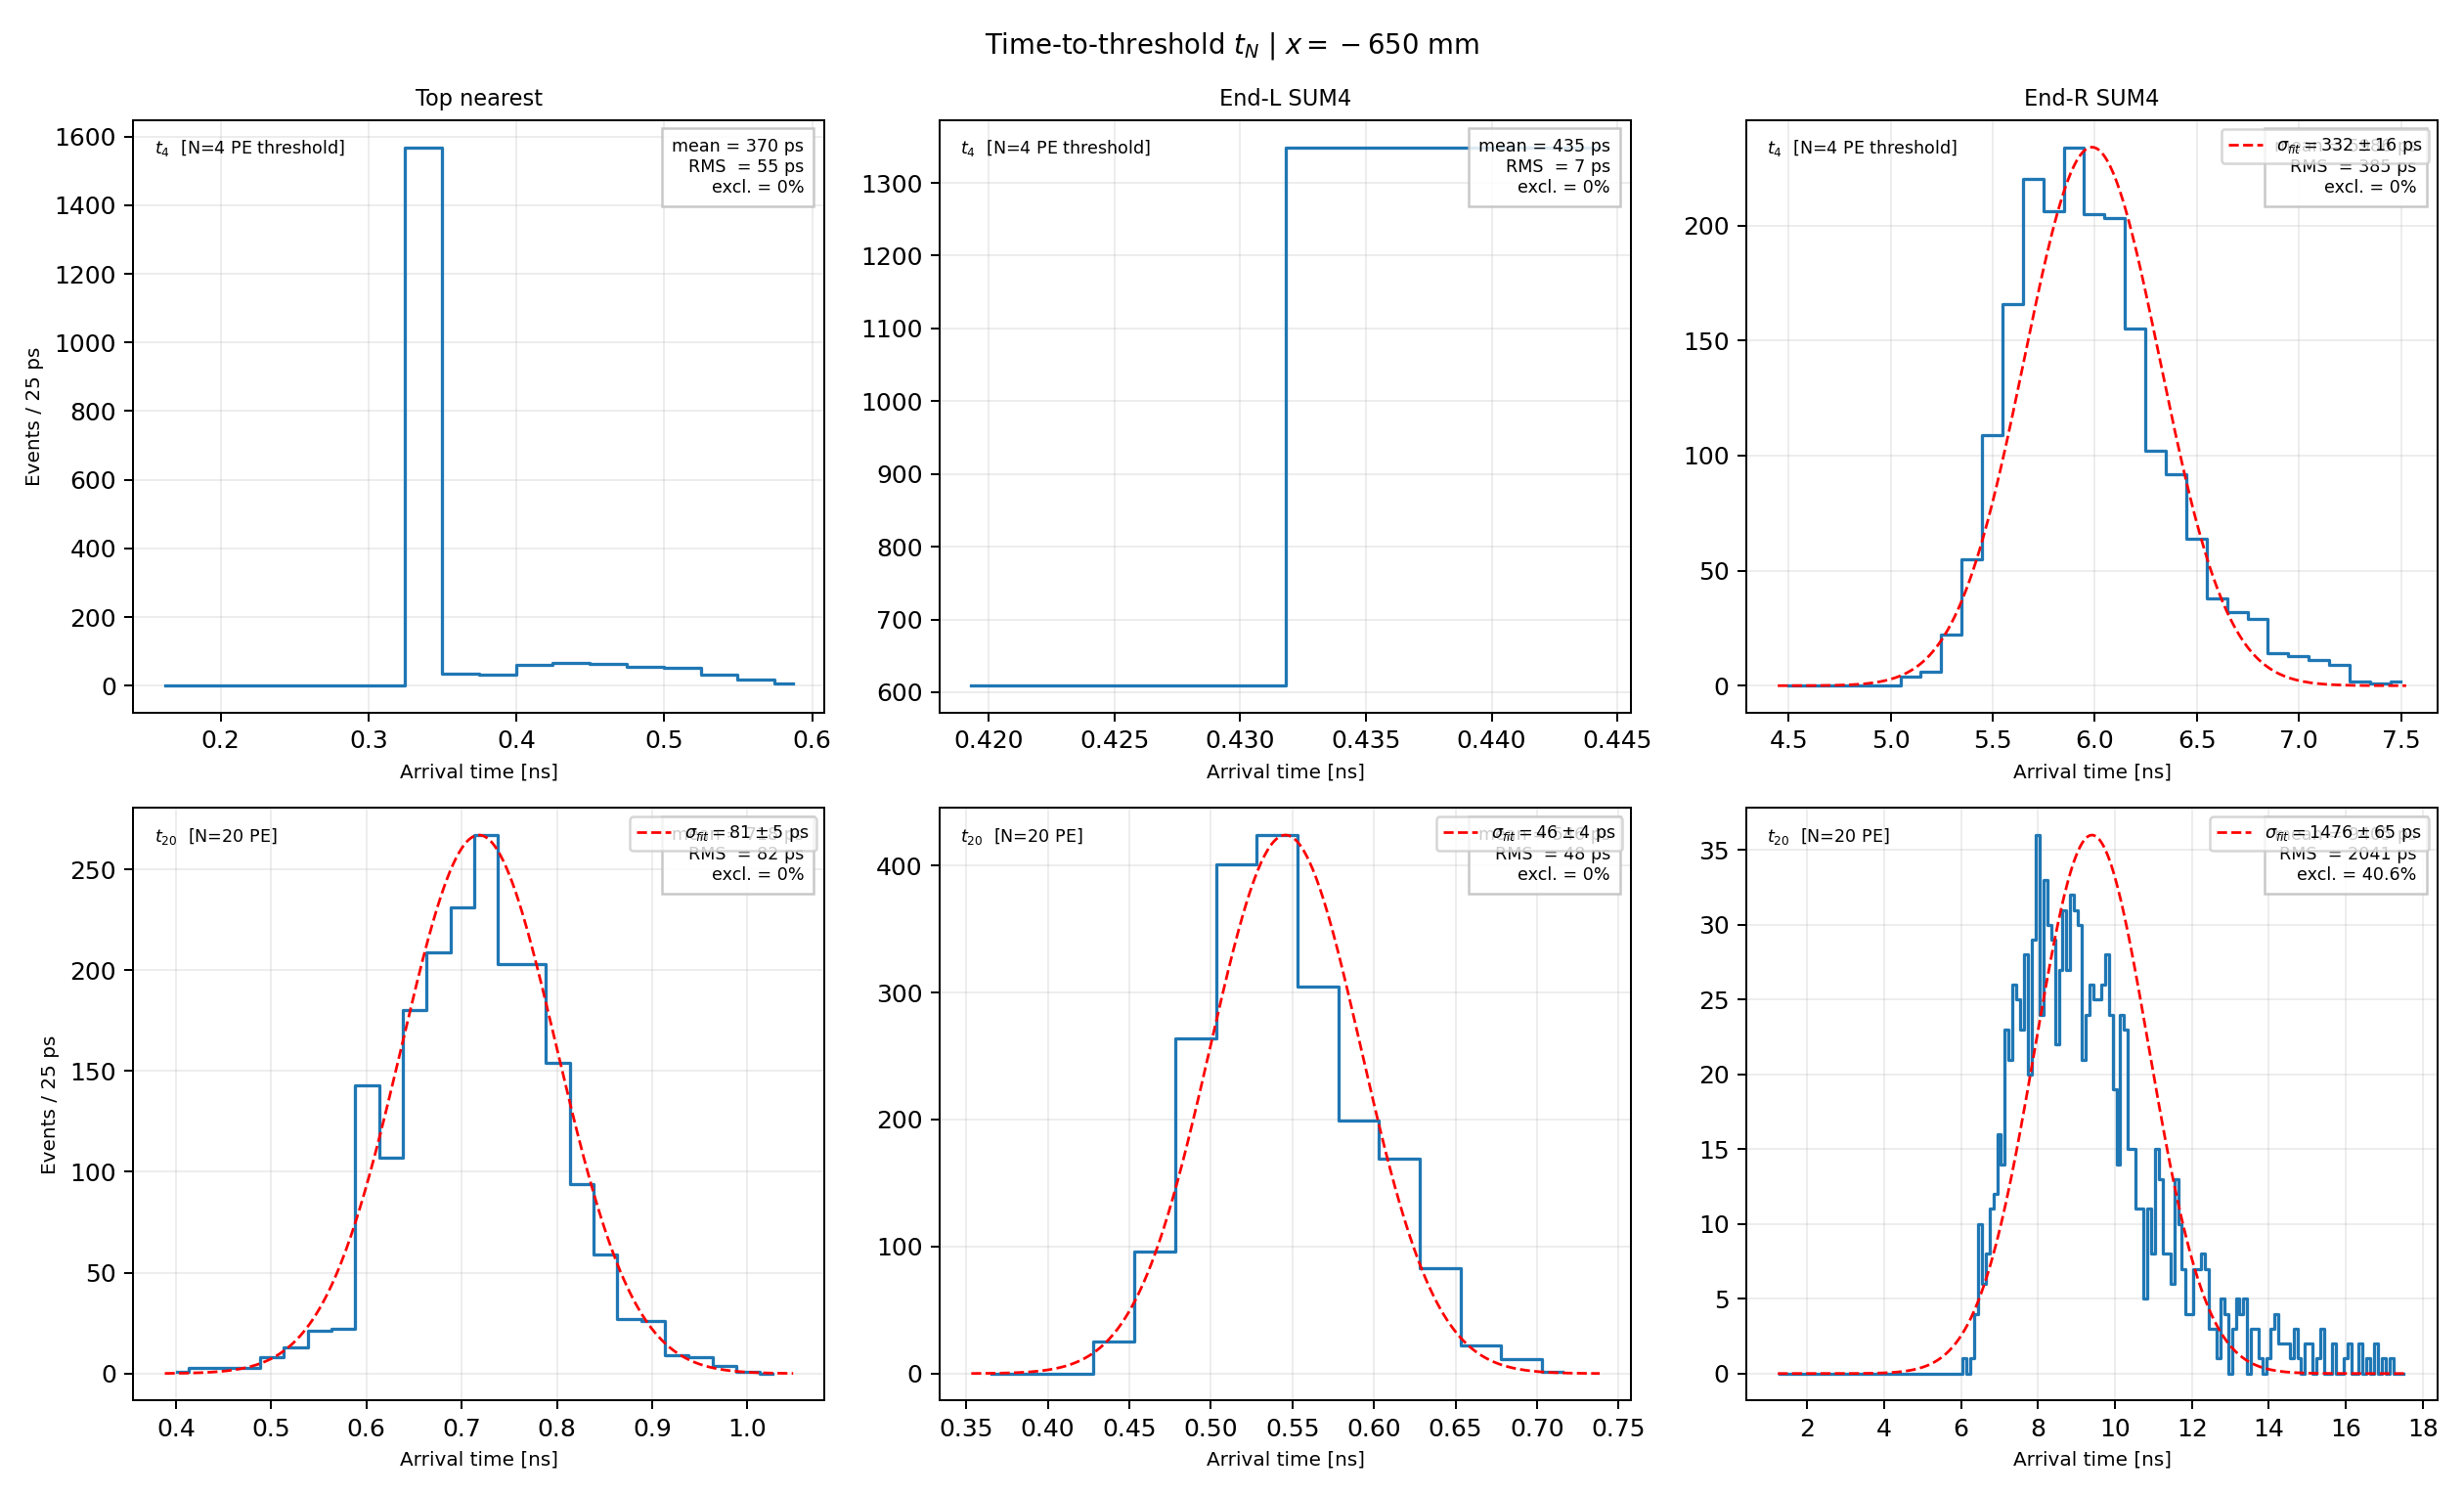
\includegraphics[width=\textwidth,height=0.84\textheight,keepaspectratio]{figs/exec12_tN_-650mm.png}
\end{frame}
\begin{frame}{Position x=-400 mm}

\begin{columns}[T]
  \column{0.52\textwidth}
  
\includegraphics[width=\textwidth]{figs/muon_-400mm_geometry.png}
  \column{0.46\textwidth}
  
\includegraphics[width=\textwidth]{figs/muon_-400mm_top_profile.png}
  \tiny
  \begin{tabular}{lr}
    \toprule Quantity & Value \\ \midrule
    End L $N_{pe}$ & $691.3\pm3.9$ \\
    End R $N_{pe}$ & $74.5\pm0.5$ \\
    Nearest Top ID & 31 (exact geometry) \\
    Nearest Top $N_{pe}$ & $411.3\pm2.3$ \\
    Nearest Top $\langle t\rangle$ &
      $2.9399\pm0.0022$ ns \\
    Nearest Top FPT & $0.34597\pm0.00021$ ns \\
    \bottomrule
  \end{tabular}
\end{columns}

\end{frame}
\begin{frame}{Run 3 $|$ x = -400 mm $|$ Photon arrival $\langle N(t)\rangle$}
\centering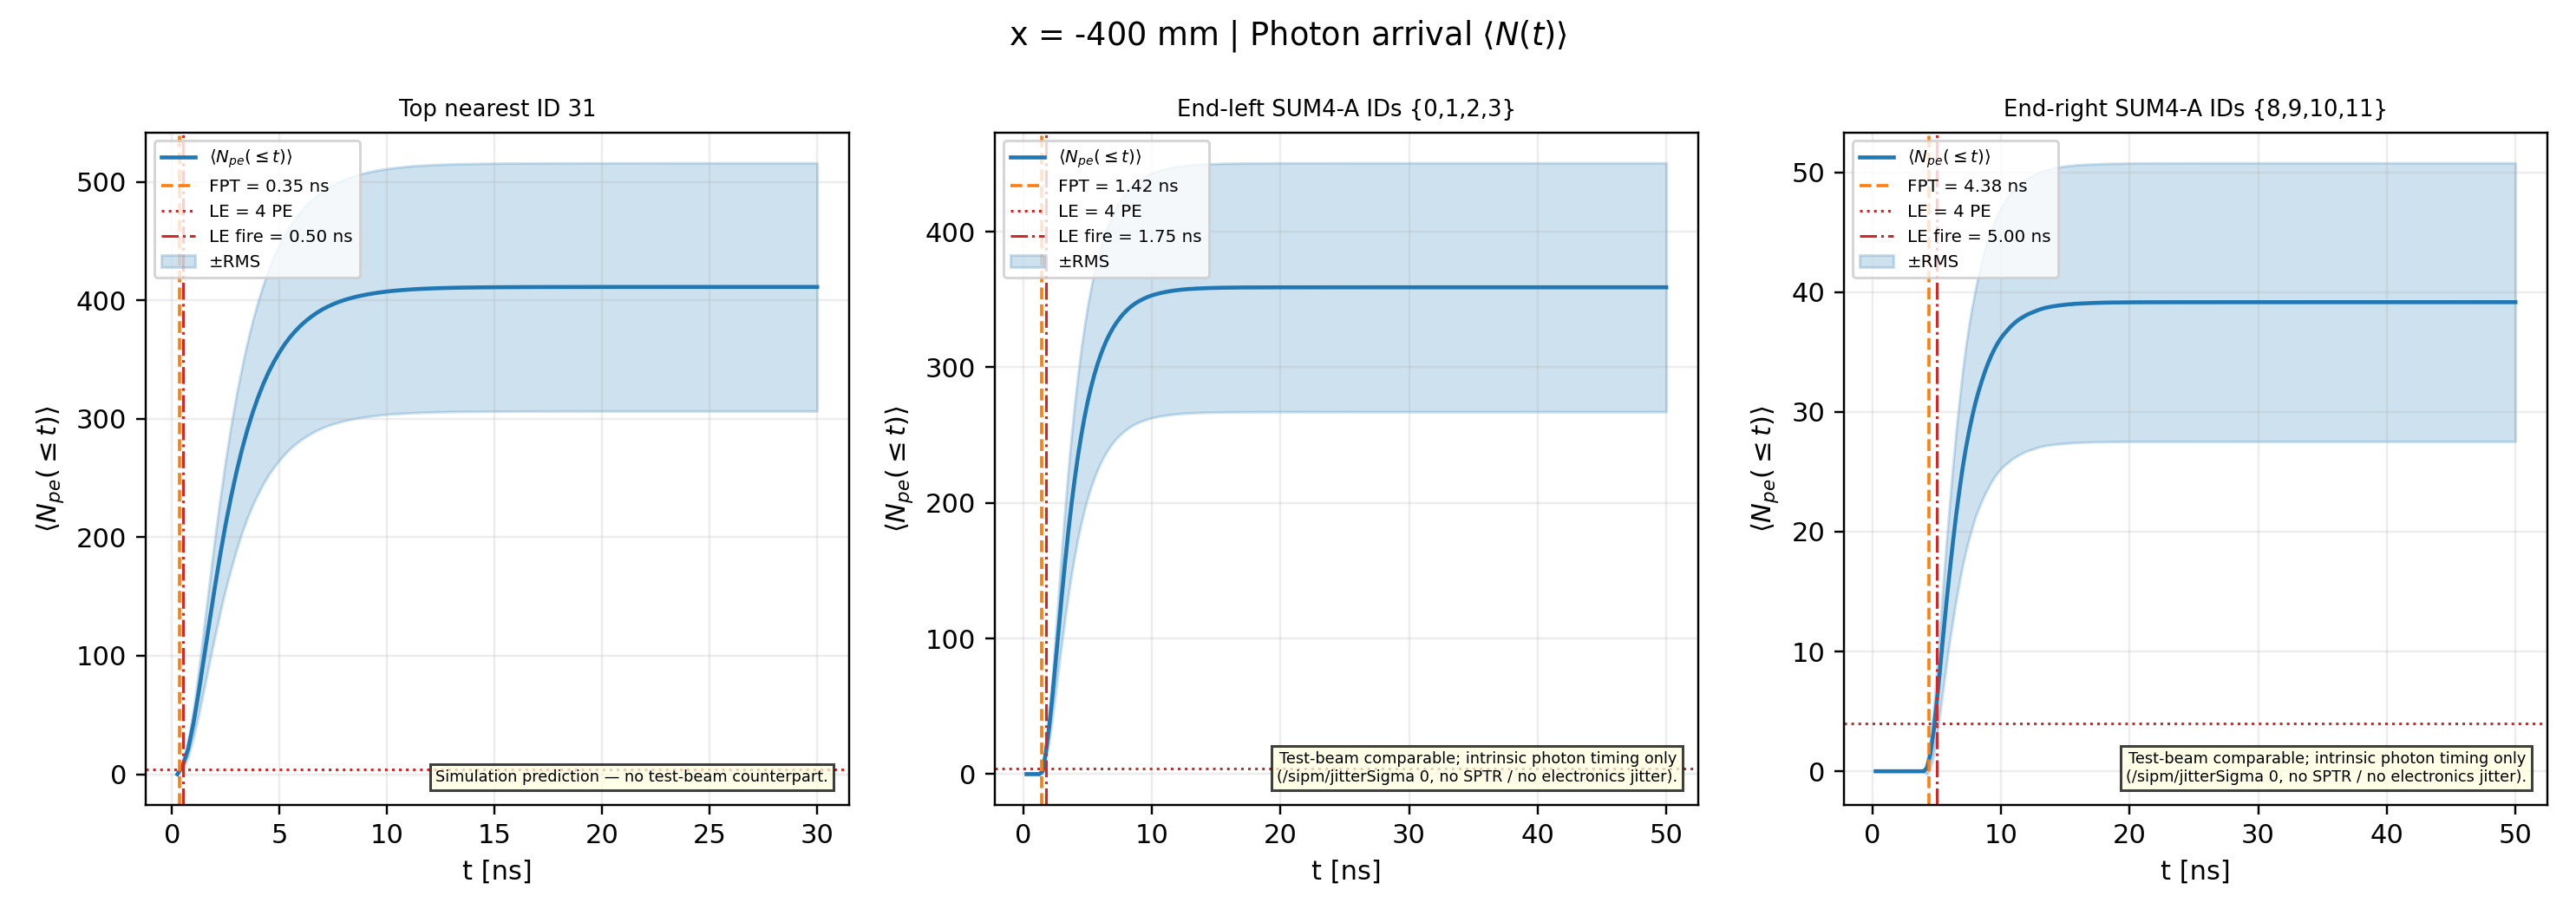
\includegraphics[width=\textwidth,height=0.78\textheight,keepaspectratio]{figs/exec11_arrival_-400mm.png}
\end{frame}
\begin{frame}{Run 3 $|$ x = -400 mm $|$ Time-to-threshold $t_N$}
\centering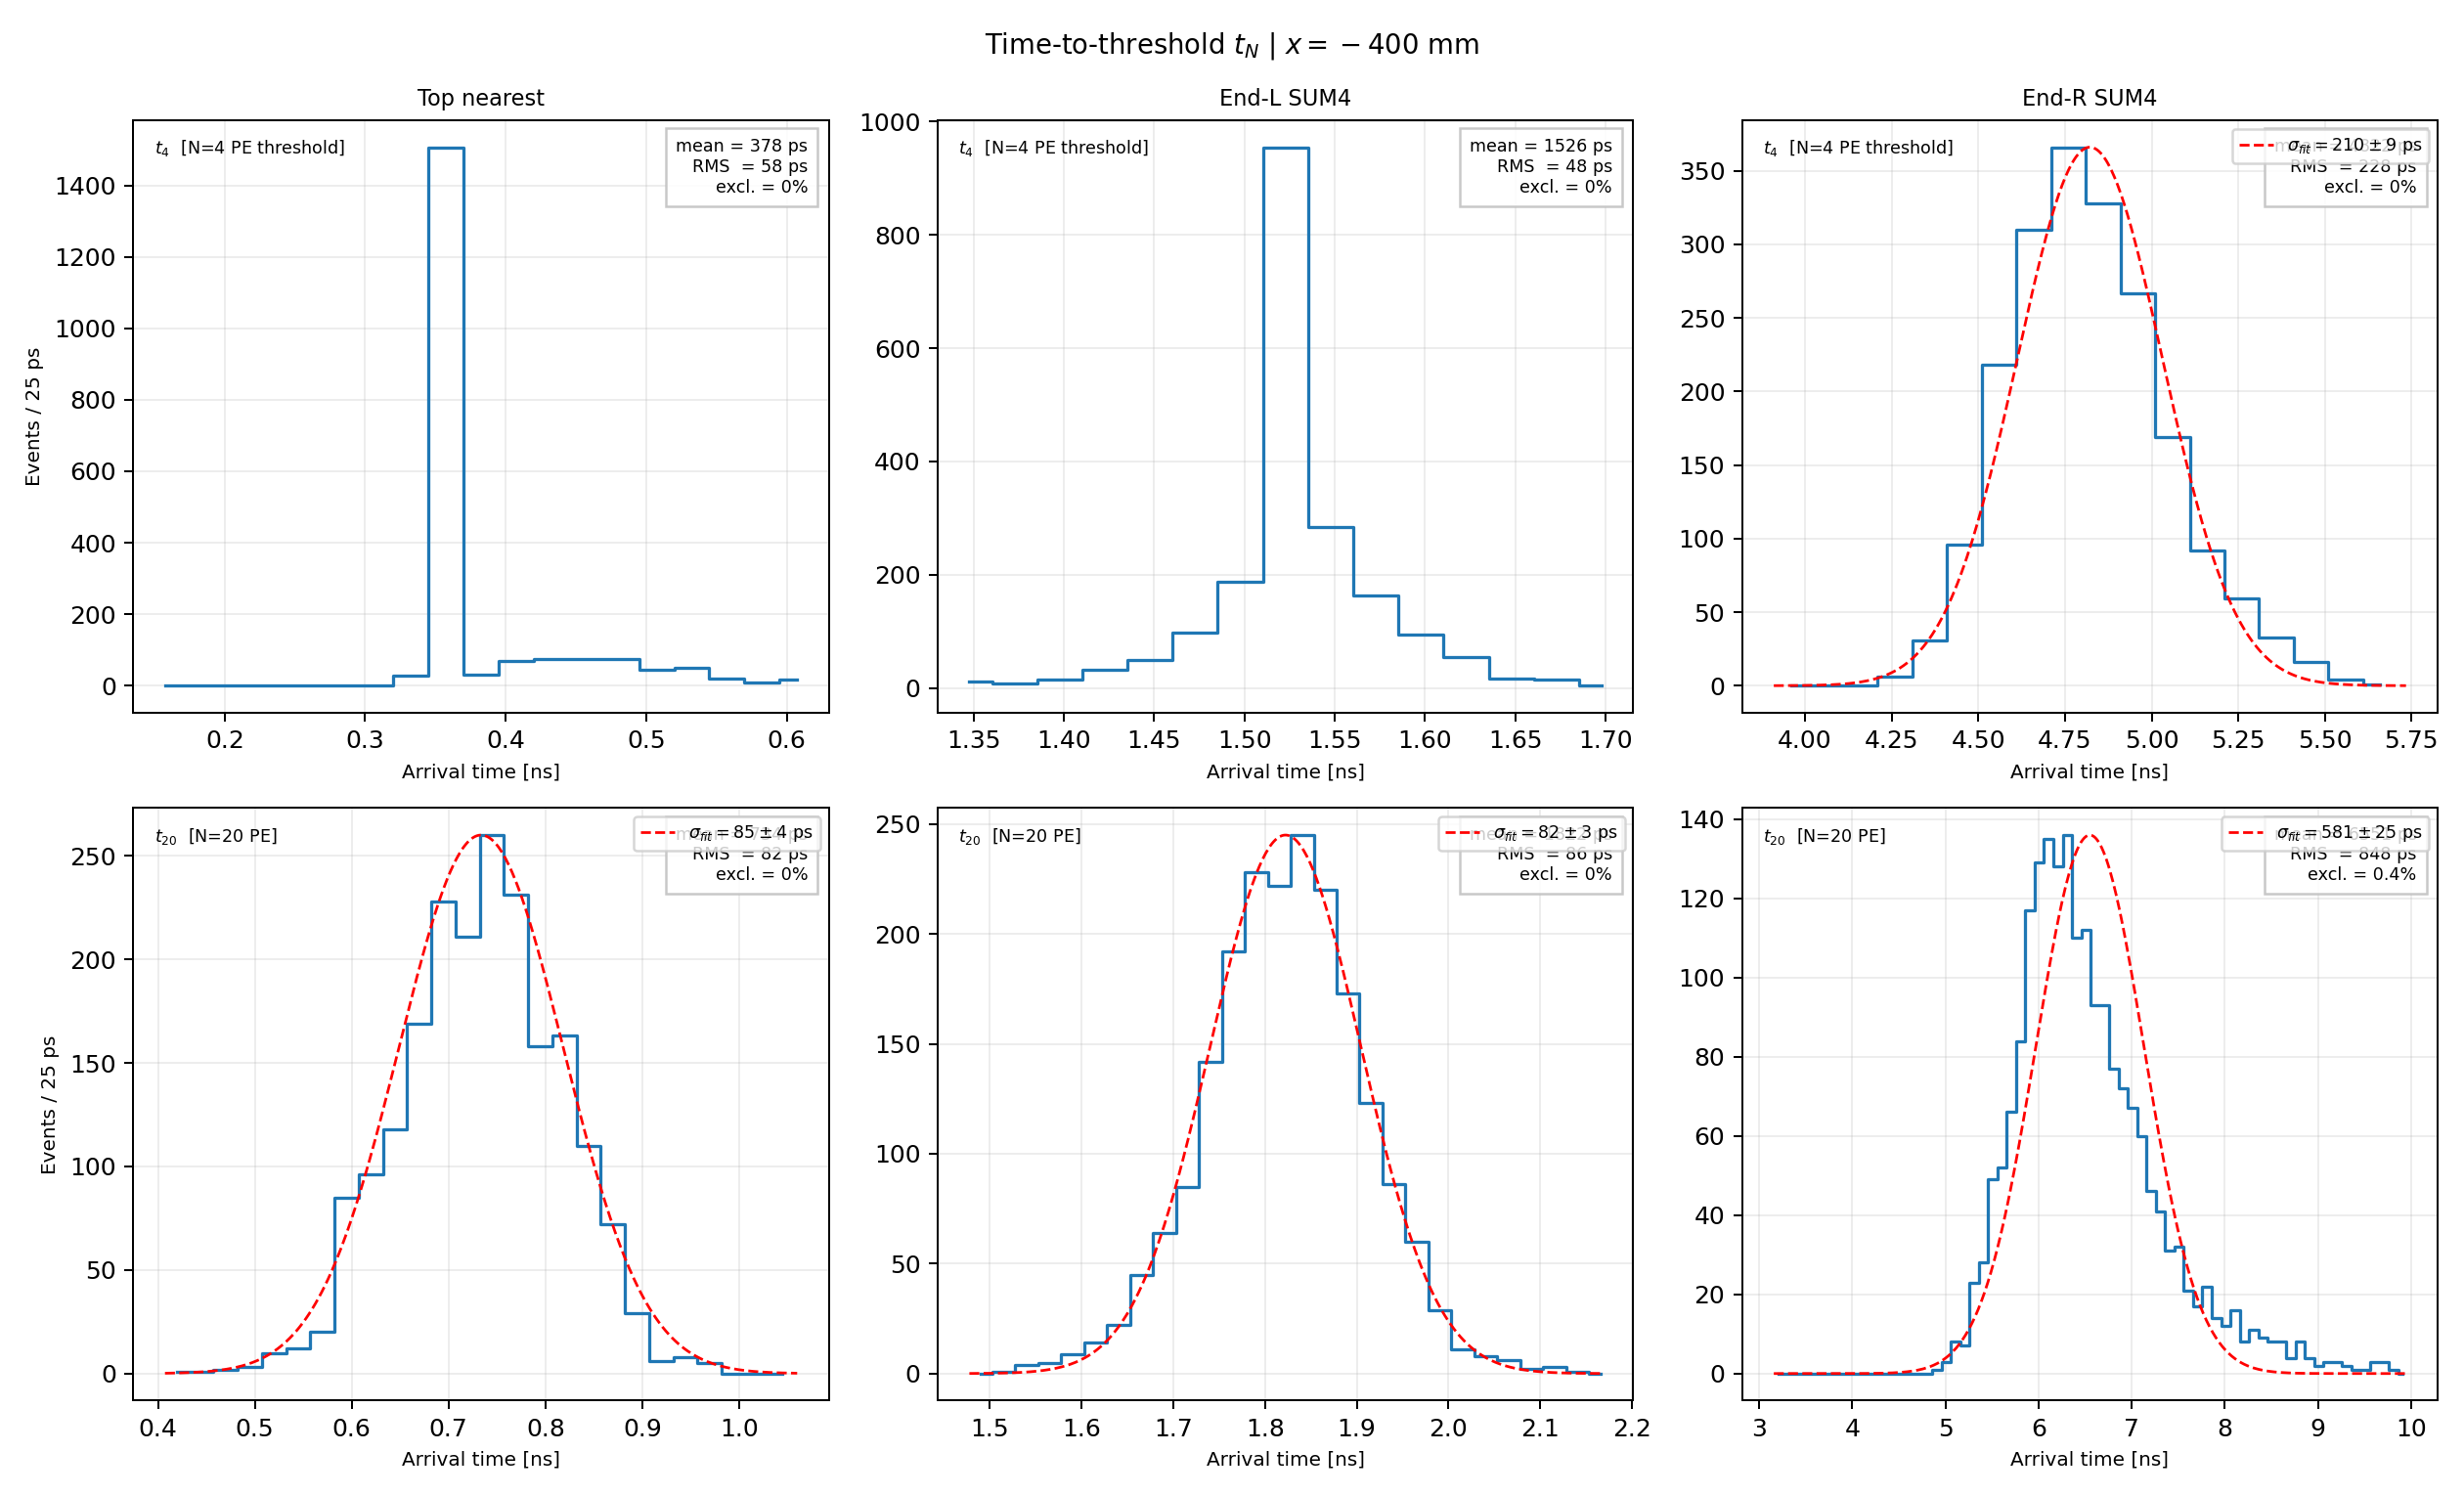
\includegraphics[width=\textwidth,height=0.84\textheight,keepaspectratio]{figs/exec12_tN_-400mm.png}
\end{frame}
\begin{frame}{Position x=0 mm}

\begin{columns}[T]
  \column{0.52\textwidth}
  
\includegraphics[width=\textwidth]{figs/muon_0mm_geometry.png}
  \column{0.46\textwidth}
  
\includegraphics[width=\textwidth]{figs/muon_0mm_top_profile.png}
  \tiny
  \begin{tabular}{lr}
    \toprule Quantity & Value \\ \midrule
    End L $N_{pe}$ & $194.4\pm1.1$ \\
    End R $N_{pe}$ & $195.2\pm1.1$ \\
    Nearest Top ID & 51 (exact geometry) \\
    Nearest Top $N_{pe}$ & $407.3\pm2.2$ \\
    Nearest Top $\langle t\rangle$ &
      $3.0030\pm0.0022$ ns \\
    Nearest Top FPT & $0.35075\pm0.00020$ ns \\
    \bottomrule
  \end{tabular}
\end{columns}

\end{frame}
\begin{frame}{Run 4 $|$ x = +0 mm $|$ Photon arrival $\langle N(t)\rangle$}
\centering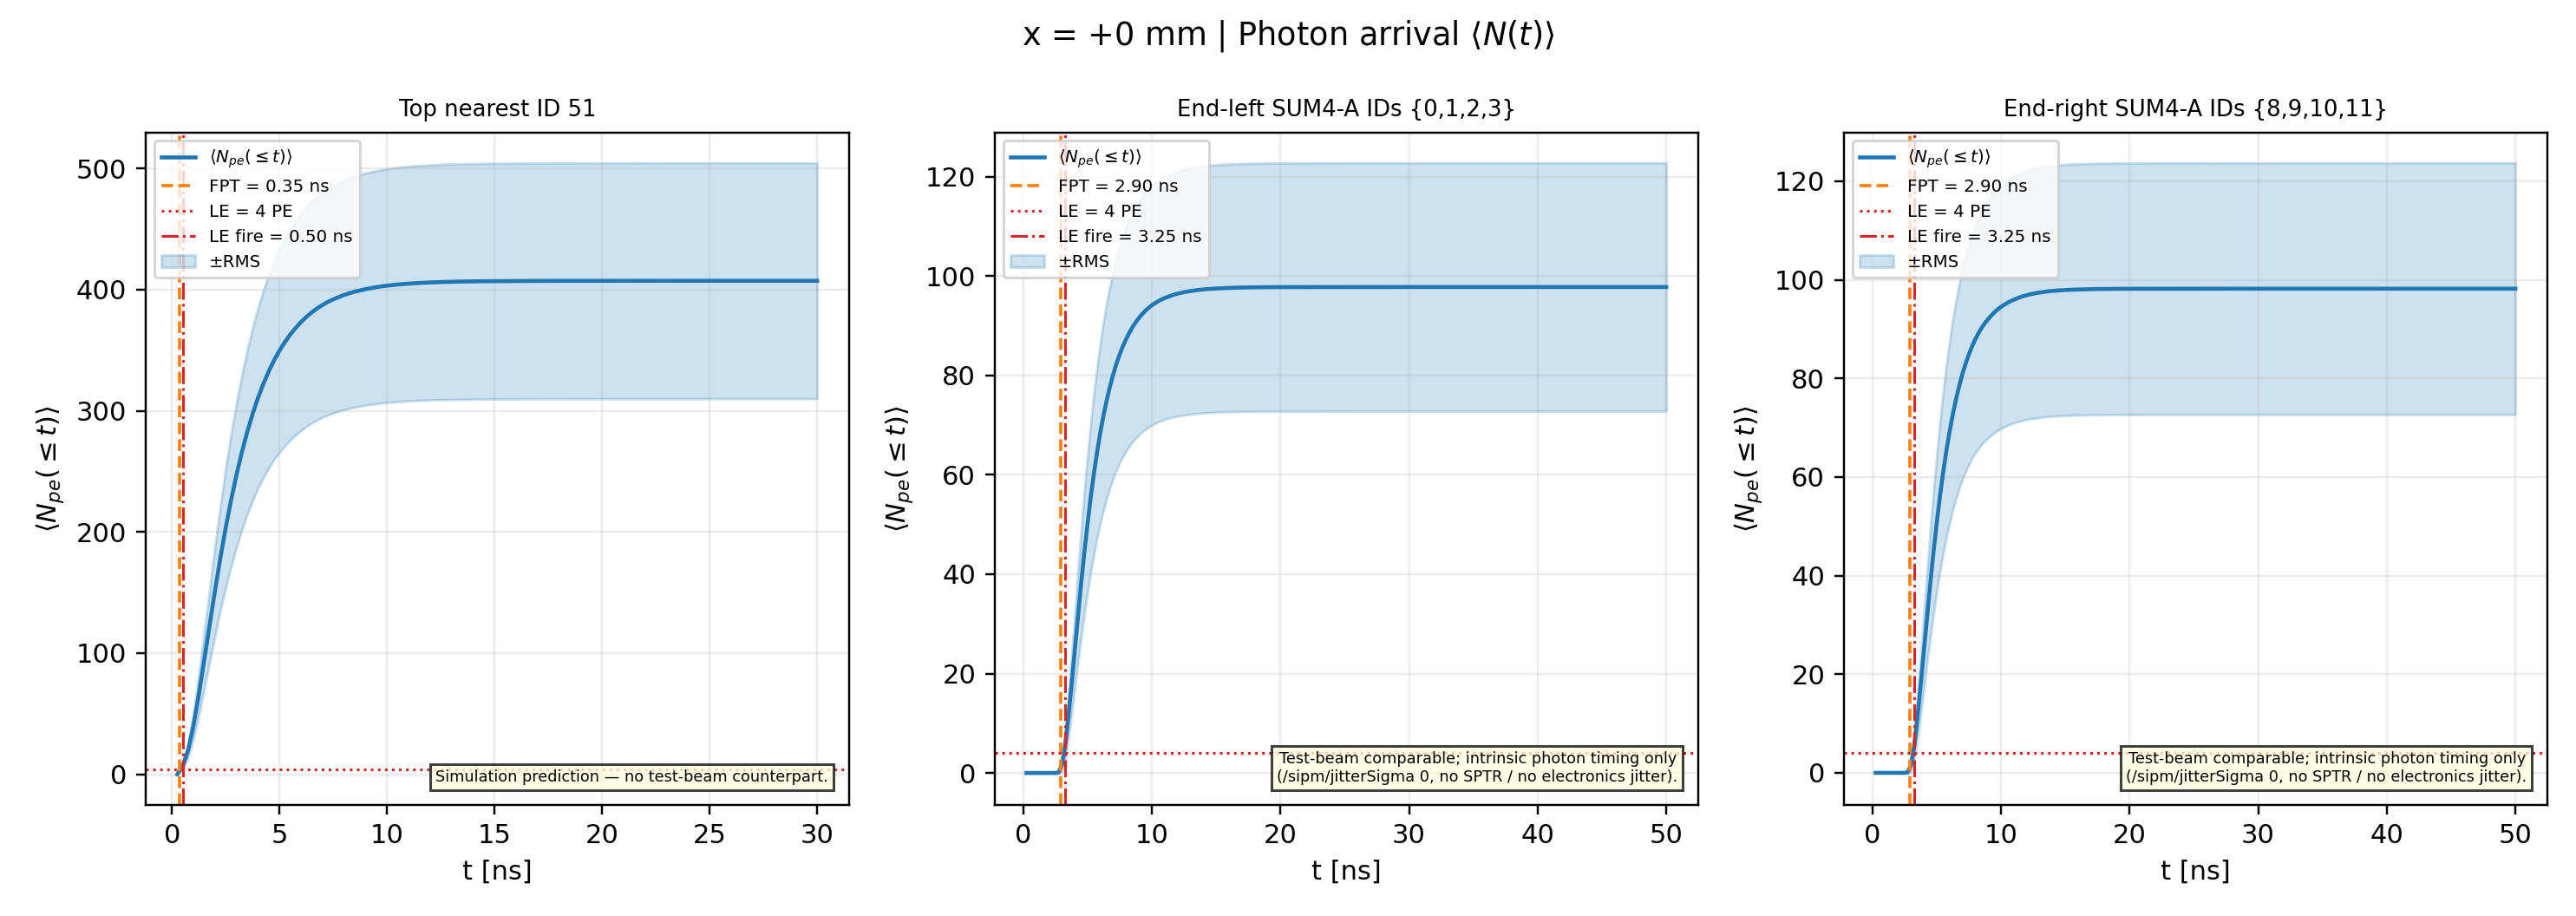
\includegraphics[width=\textwidth,height=0.78\textheight,keepaspectratio]{figs/exec11_arrival_0mm.png}
\end{frame}
\begin{frame}{Run 4 $|$ x = +0 mm $|$ Time-to-threshold $t_N$}
\centering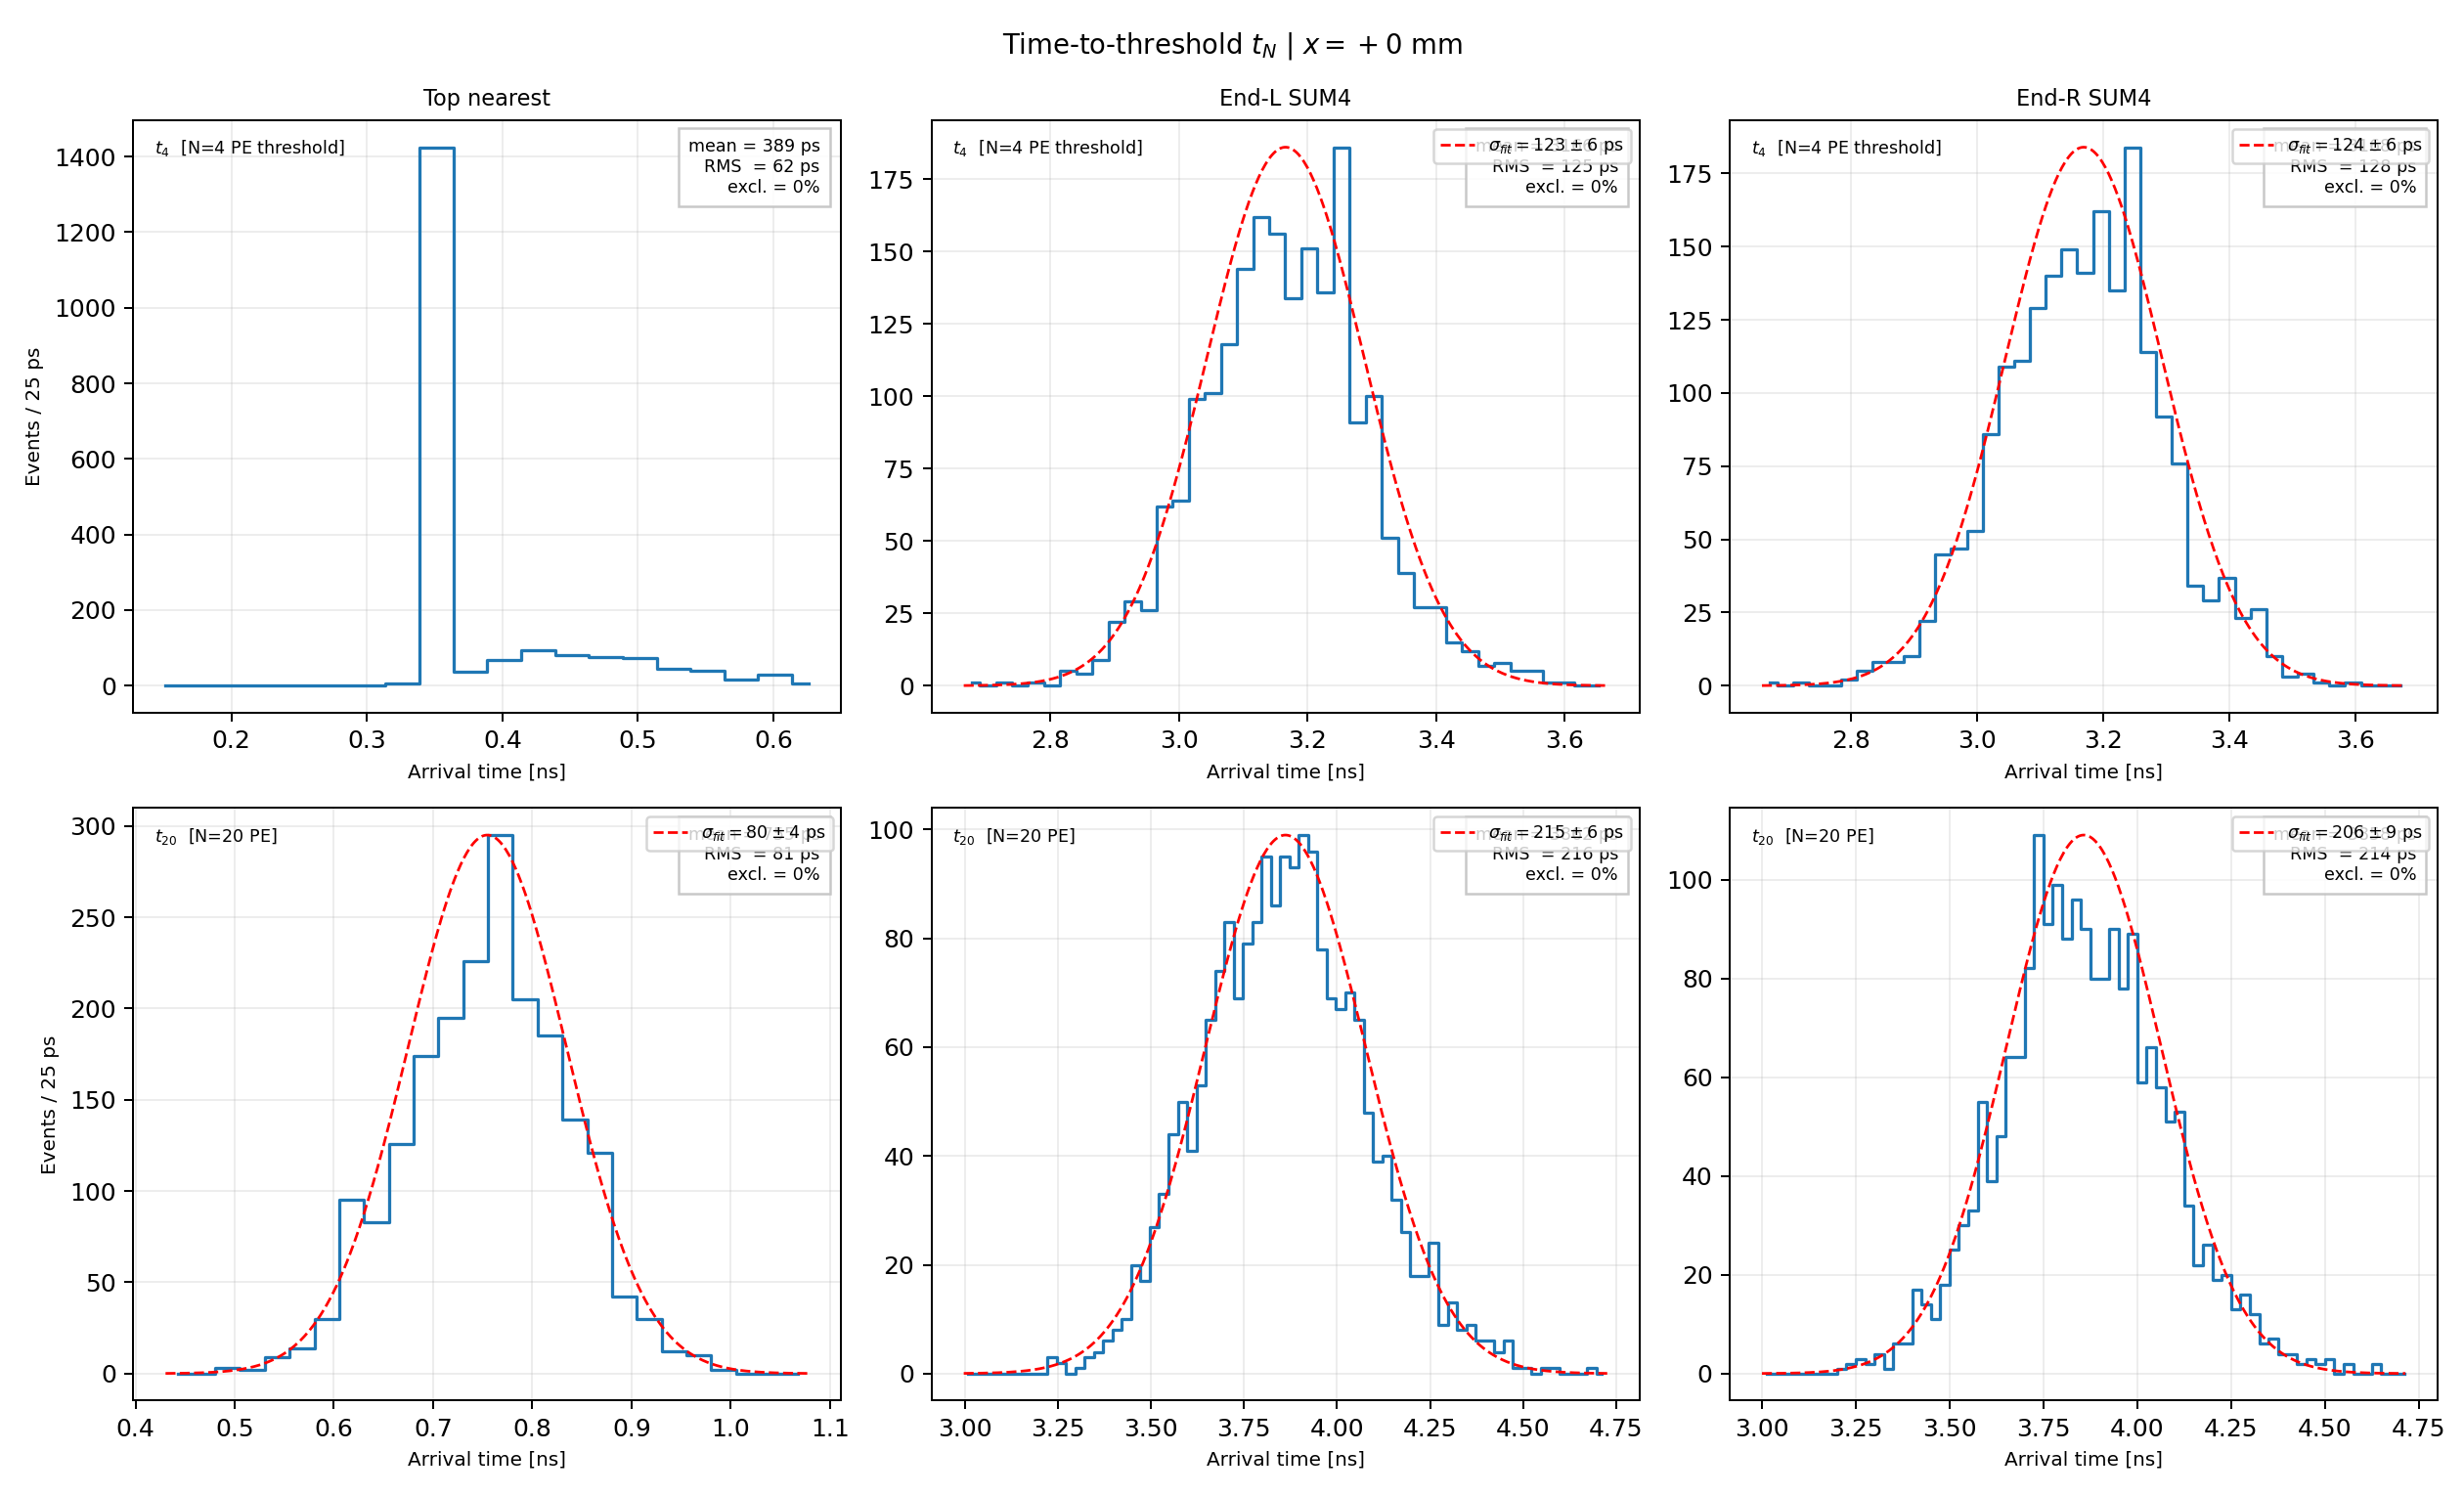
\includegraphics[width=\textwidth,height=0.84\textheight,keepaspectratio]{figs/exec12_tN_0mm.png}
\end{frame}
\begin{frame}{Position x=400 mm}

\begin{columns}[T]
  \column{0.52\textwidth}
  
\includegraphics[width=\textwidth]{figs/muon_400mm_geometry.png}
  \column{0.46\textwidth}
  
\includegraphics[width=\textwidth]{figs/muon_400mm_top_profile.png}
  \tiny
  \begin{tabular}{lr}
    \toprule Quantity & Value \\ \midrule
    End L $N_{pe}$ & $75.0\pm0.5$ \\
    End R $N_{pe}$ & $692.5\pm4.0$ \\
    Nearest Top ID & 70 (exact geometry) \\
    Nearest Top $N_{pe}$ & $411.4\pm2.4$ \\
    Nearest Top $\langle t\rangle$ &
      $2.9433\pm0.0022$ ns \\
    Nearest Top FPT & $0.34598\pm0.00022$ ns \\
    \bottomrule
  \end{tabular}
\end{columns}

\end{frame}
\begin{frame}{Run 5 $|$ x = +400 mm $|$ Photon arrival $\langle N(t)\rangle$}
\centering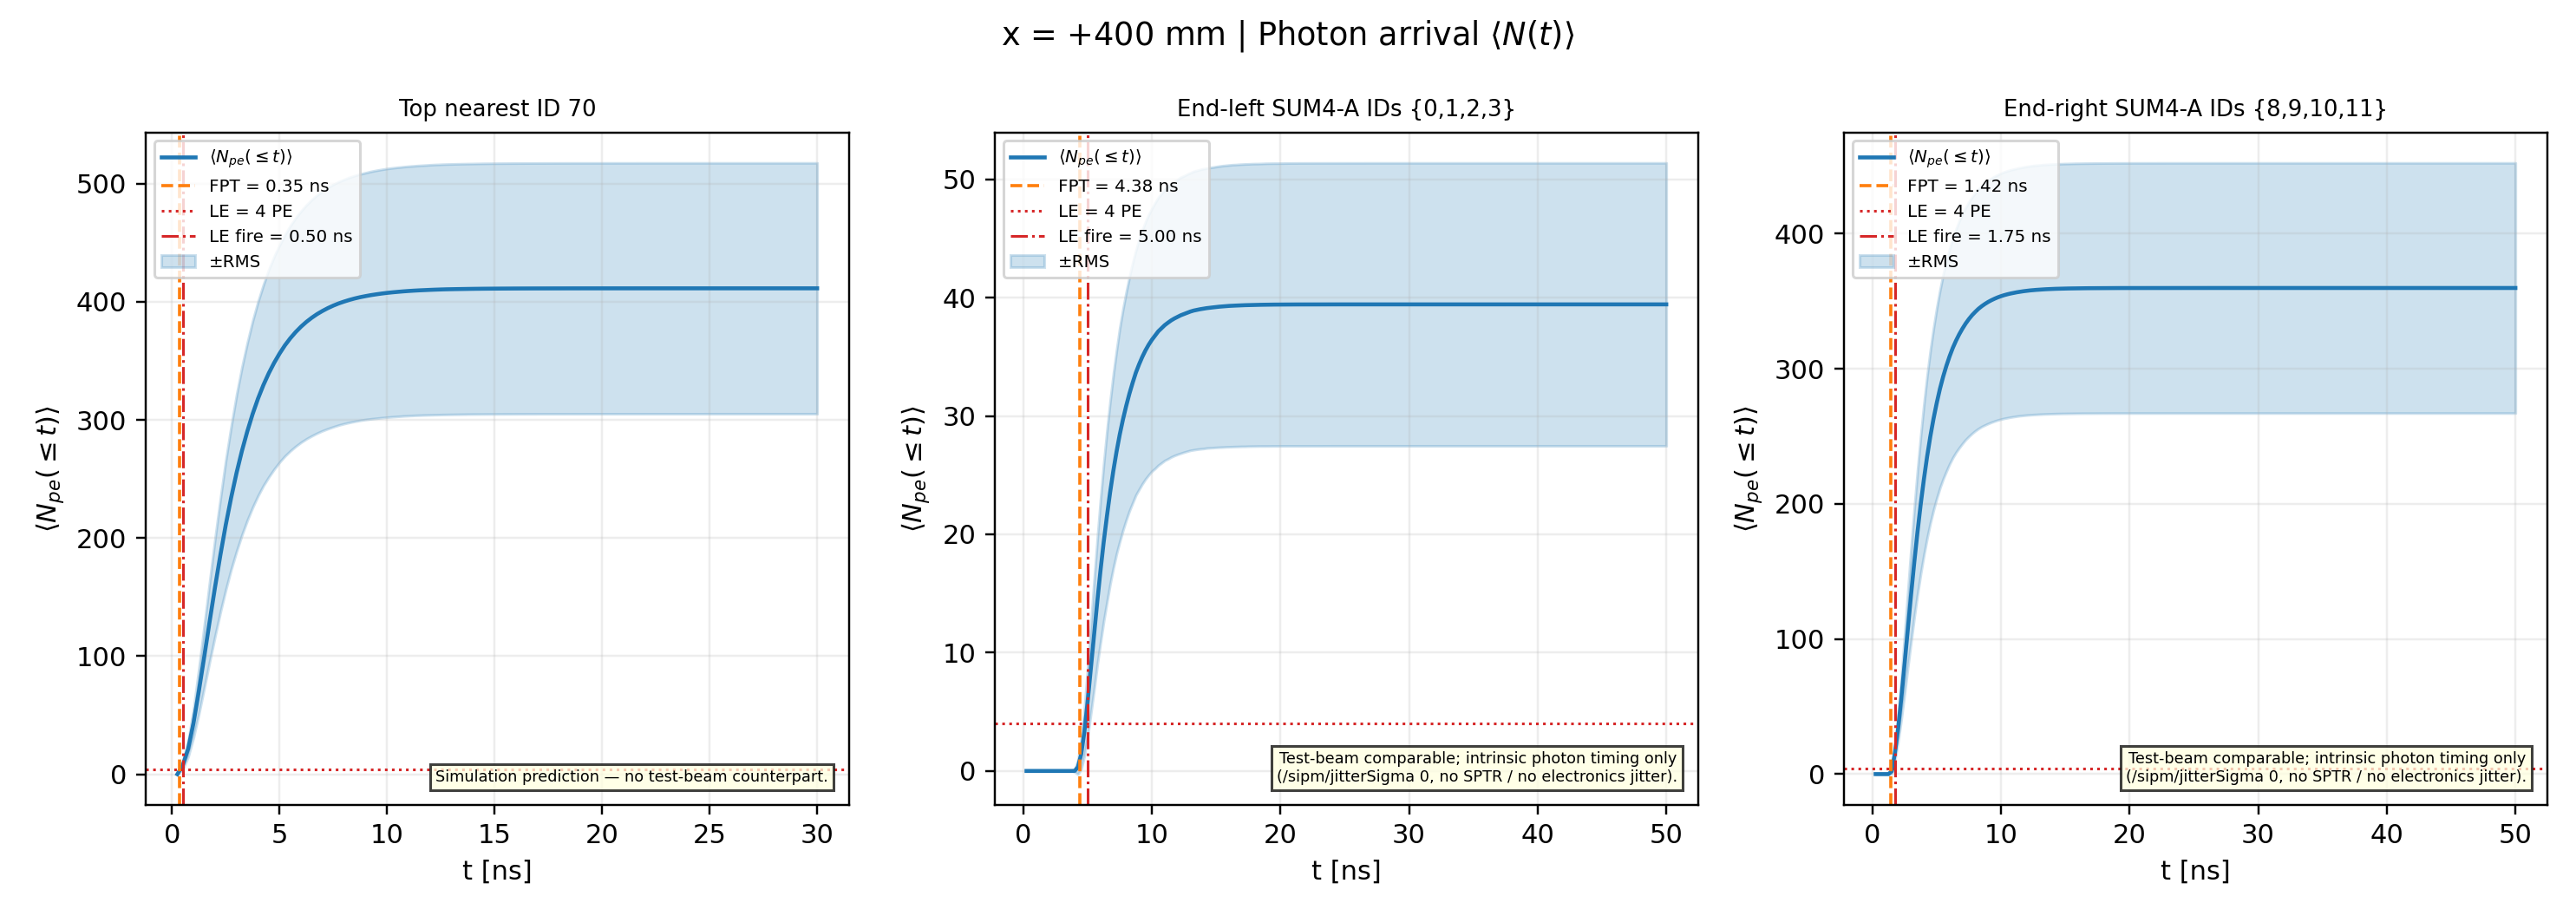
\includegraphics[width=\textwidth,height=0.78\textheight,keepaspectratio]{figs/exec11_arrival_400mm.png}
\end{frame}
\begin{frame}{Run 5 $|$ x = +400 mm $|$ Time-to-threshold $t_N$}
\centering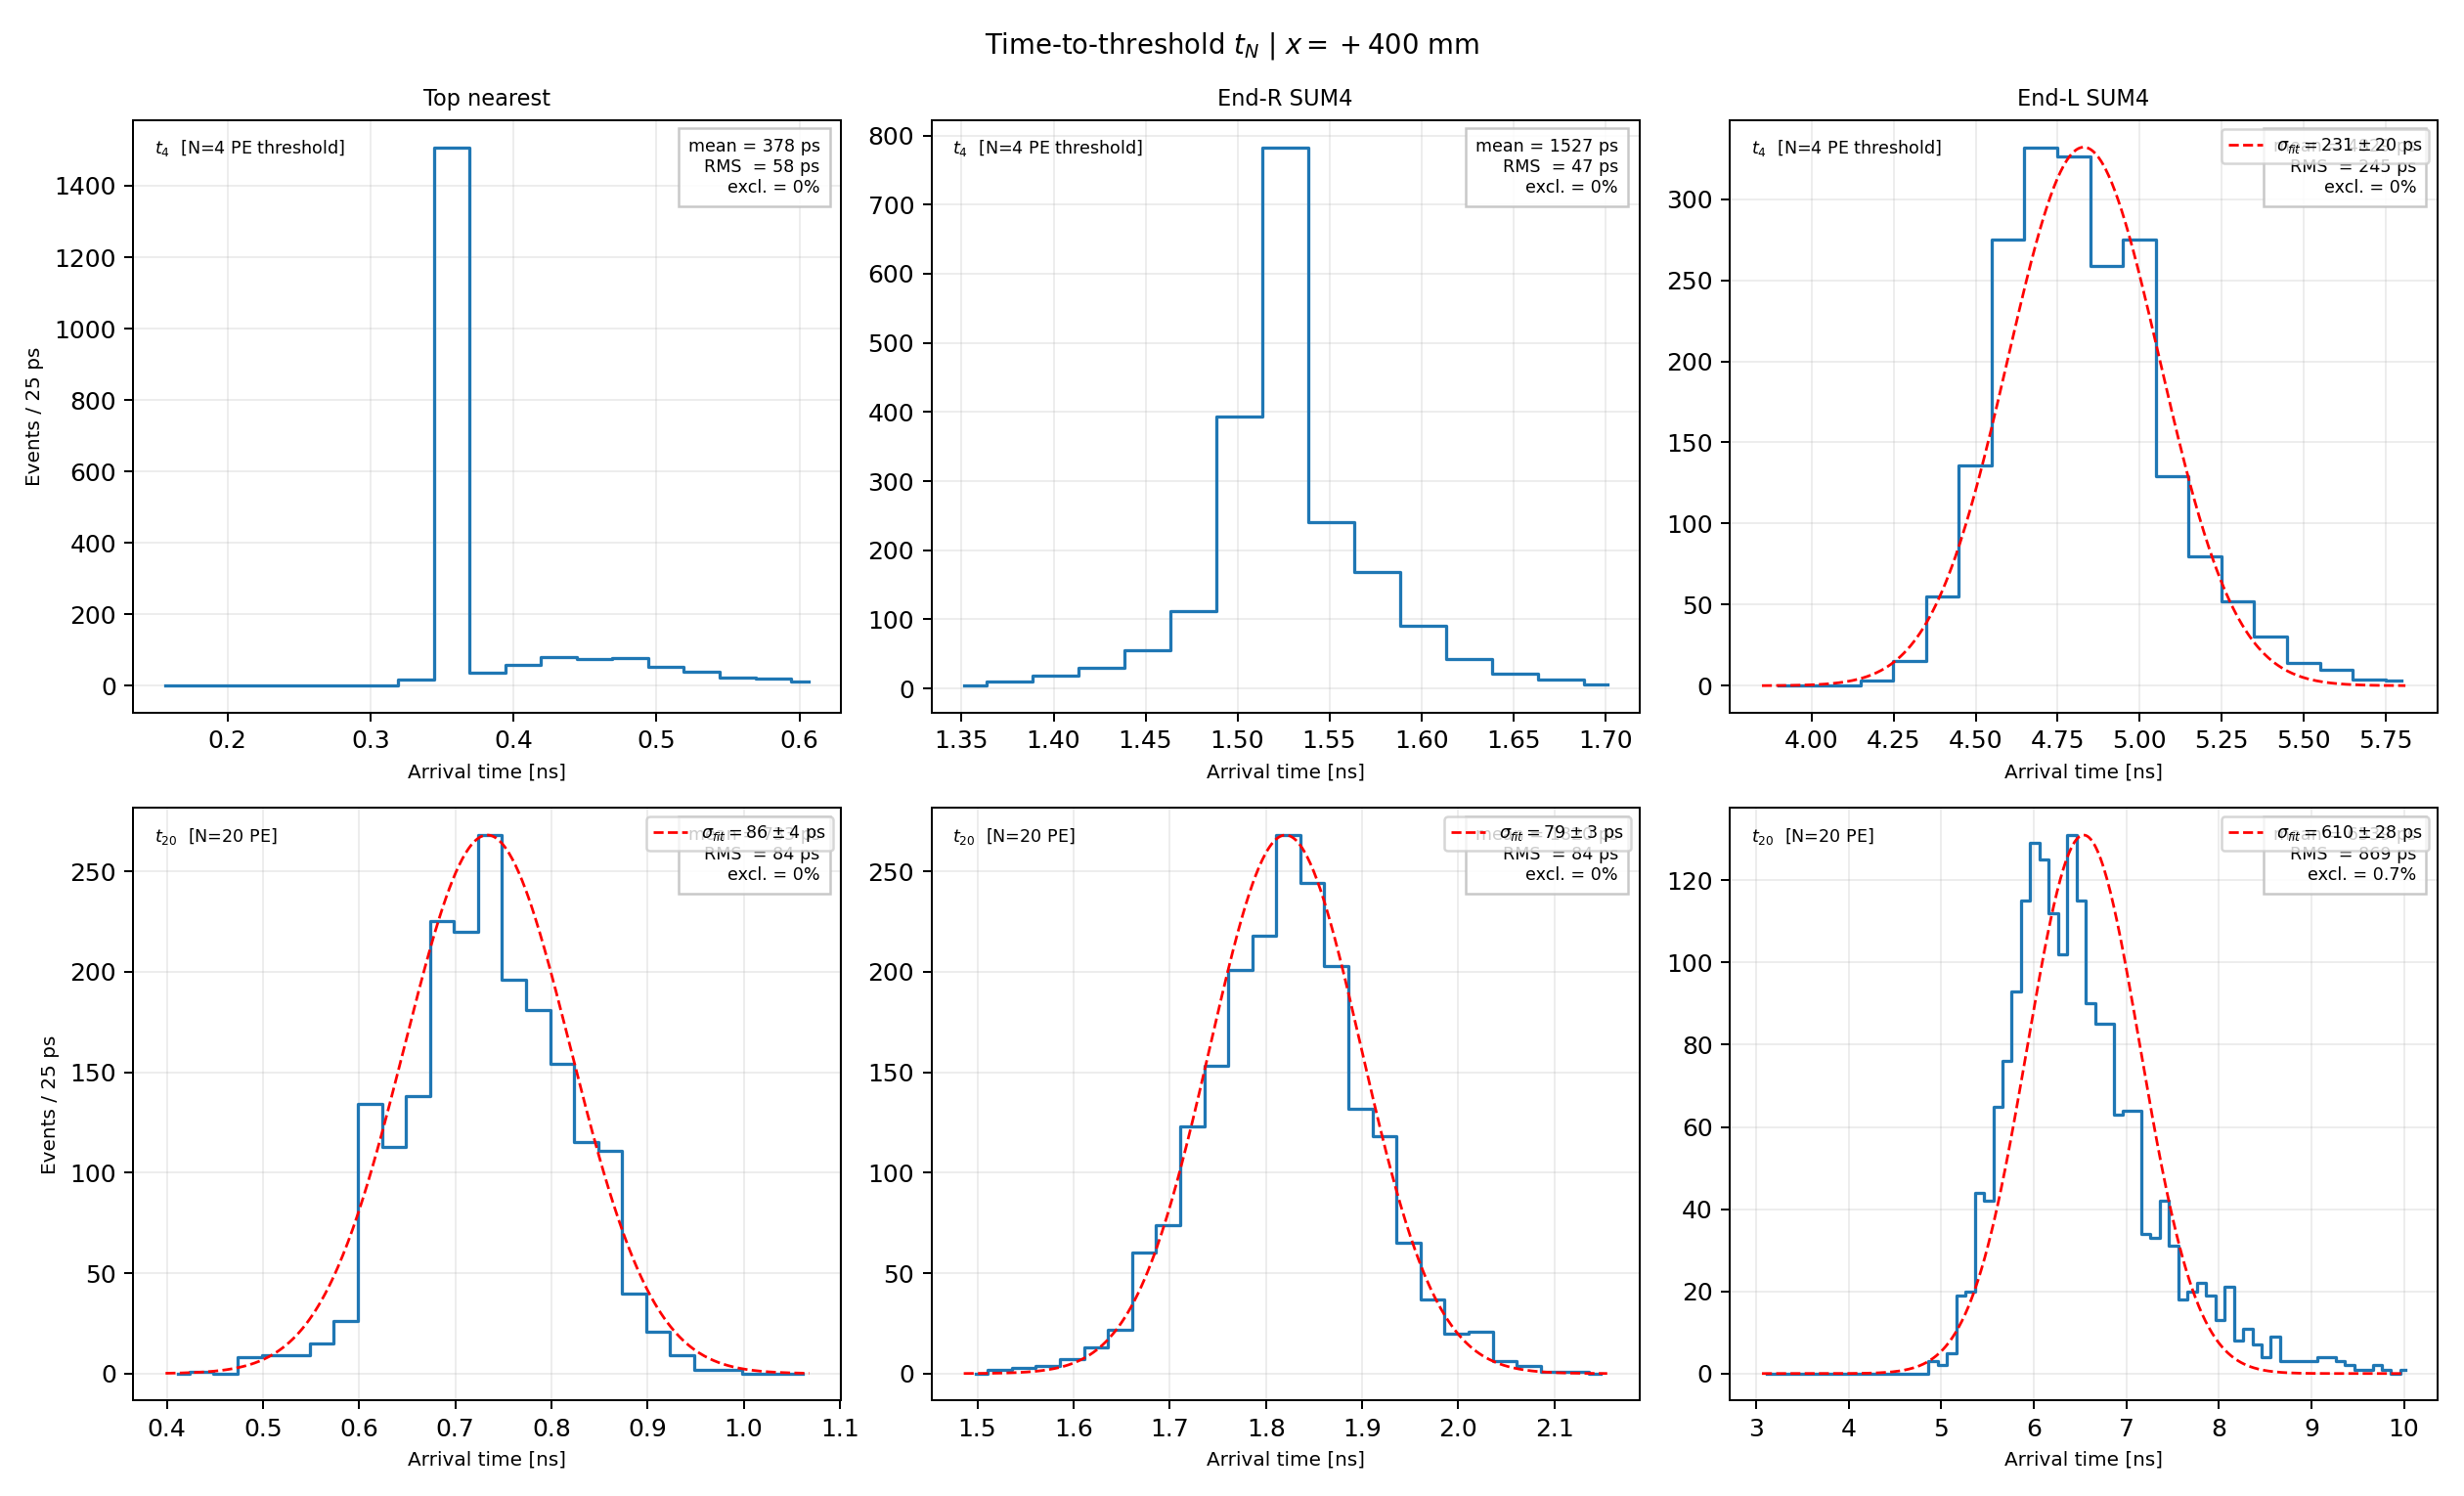
\includegraphics[width=\textwidth,height=0.84\textheight,keepaspectratio]{figs/exec12_tN_400mm.png}
\end{frame}
\begin{frame}{Position x=650 mm}

\begin{columns}[T]
  \column{0.52\textwidth}
  
\includegraphics[width=\textwidth]{figs/muon_650mm_geometry.png}
  \column{0.46\textwidth}
  
\includegraphics[width=\textwidth]{figs/muon_650mm_top_profile.png}
  \tiny
  \begin{tabular}{lr}
    \toprule Quantity & Value \\ \midrule
    End L $N_{pe}$ & $44.4\pm0.3$ \\
    End R $N_{pe}$ & $2357.1\pm13.0$ \\
    Nearest Top ID & 83 (window-track exception) \\
    Nearest Top $N_{pe}$ & $350.9\pm2.1$ \\
    Nearest Top $\langle t\rangle$ &
      $2.7803\pm0.0023$ ns \\
    Nearest Top FPT & $0.34268\pm0.00021$ ns \\
    \bottomrule
  \end{tabular}
\end{columns}

\end{frame}
\begin{frame}{Run 6 $|$ x = +650 mm $|$ Photon arrival $\langle N(t)\rangle$}
\centering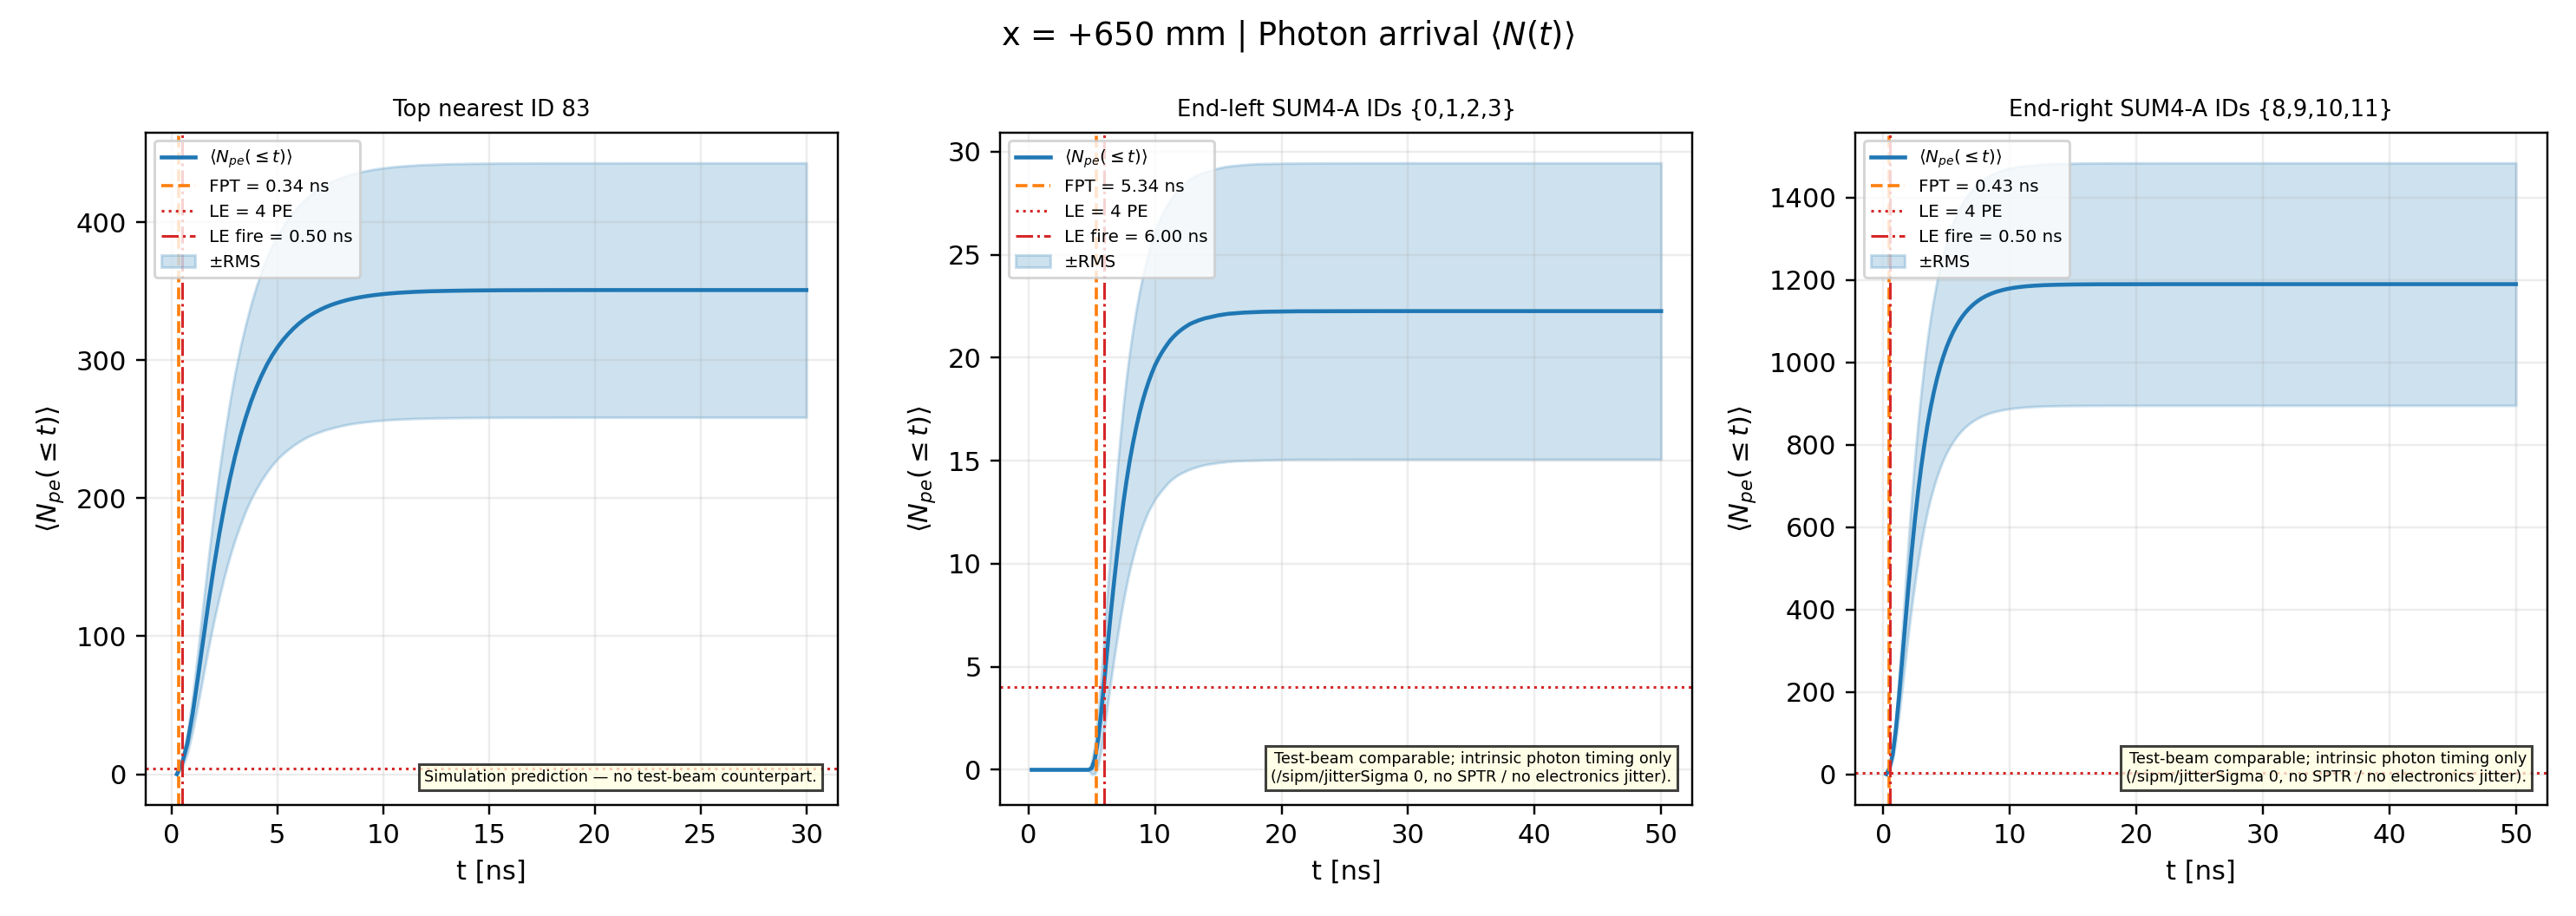
\includegraphics[width=\textwidth,height=0.78\textheight,keepaspectratio]{figs/exec11_arrival_650mm.png}
\end{frame}
\begin{frame}{Run 6 $|$ x = +650 mm $|$ Time-to-threshold $t_N$}
\centering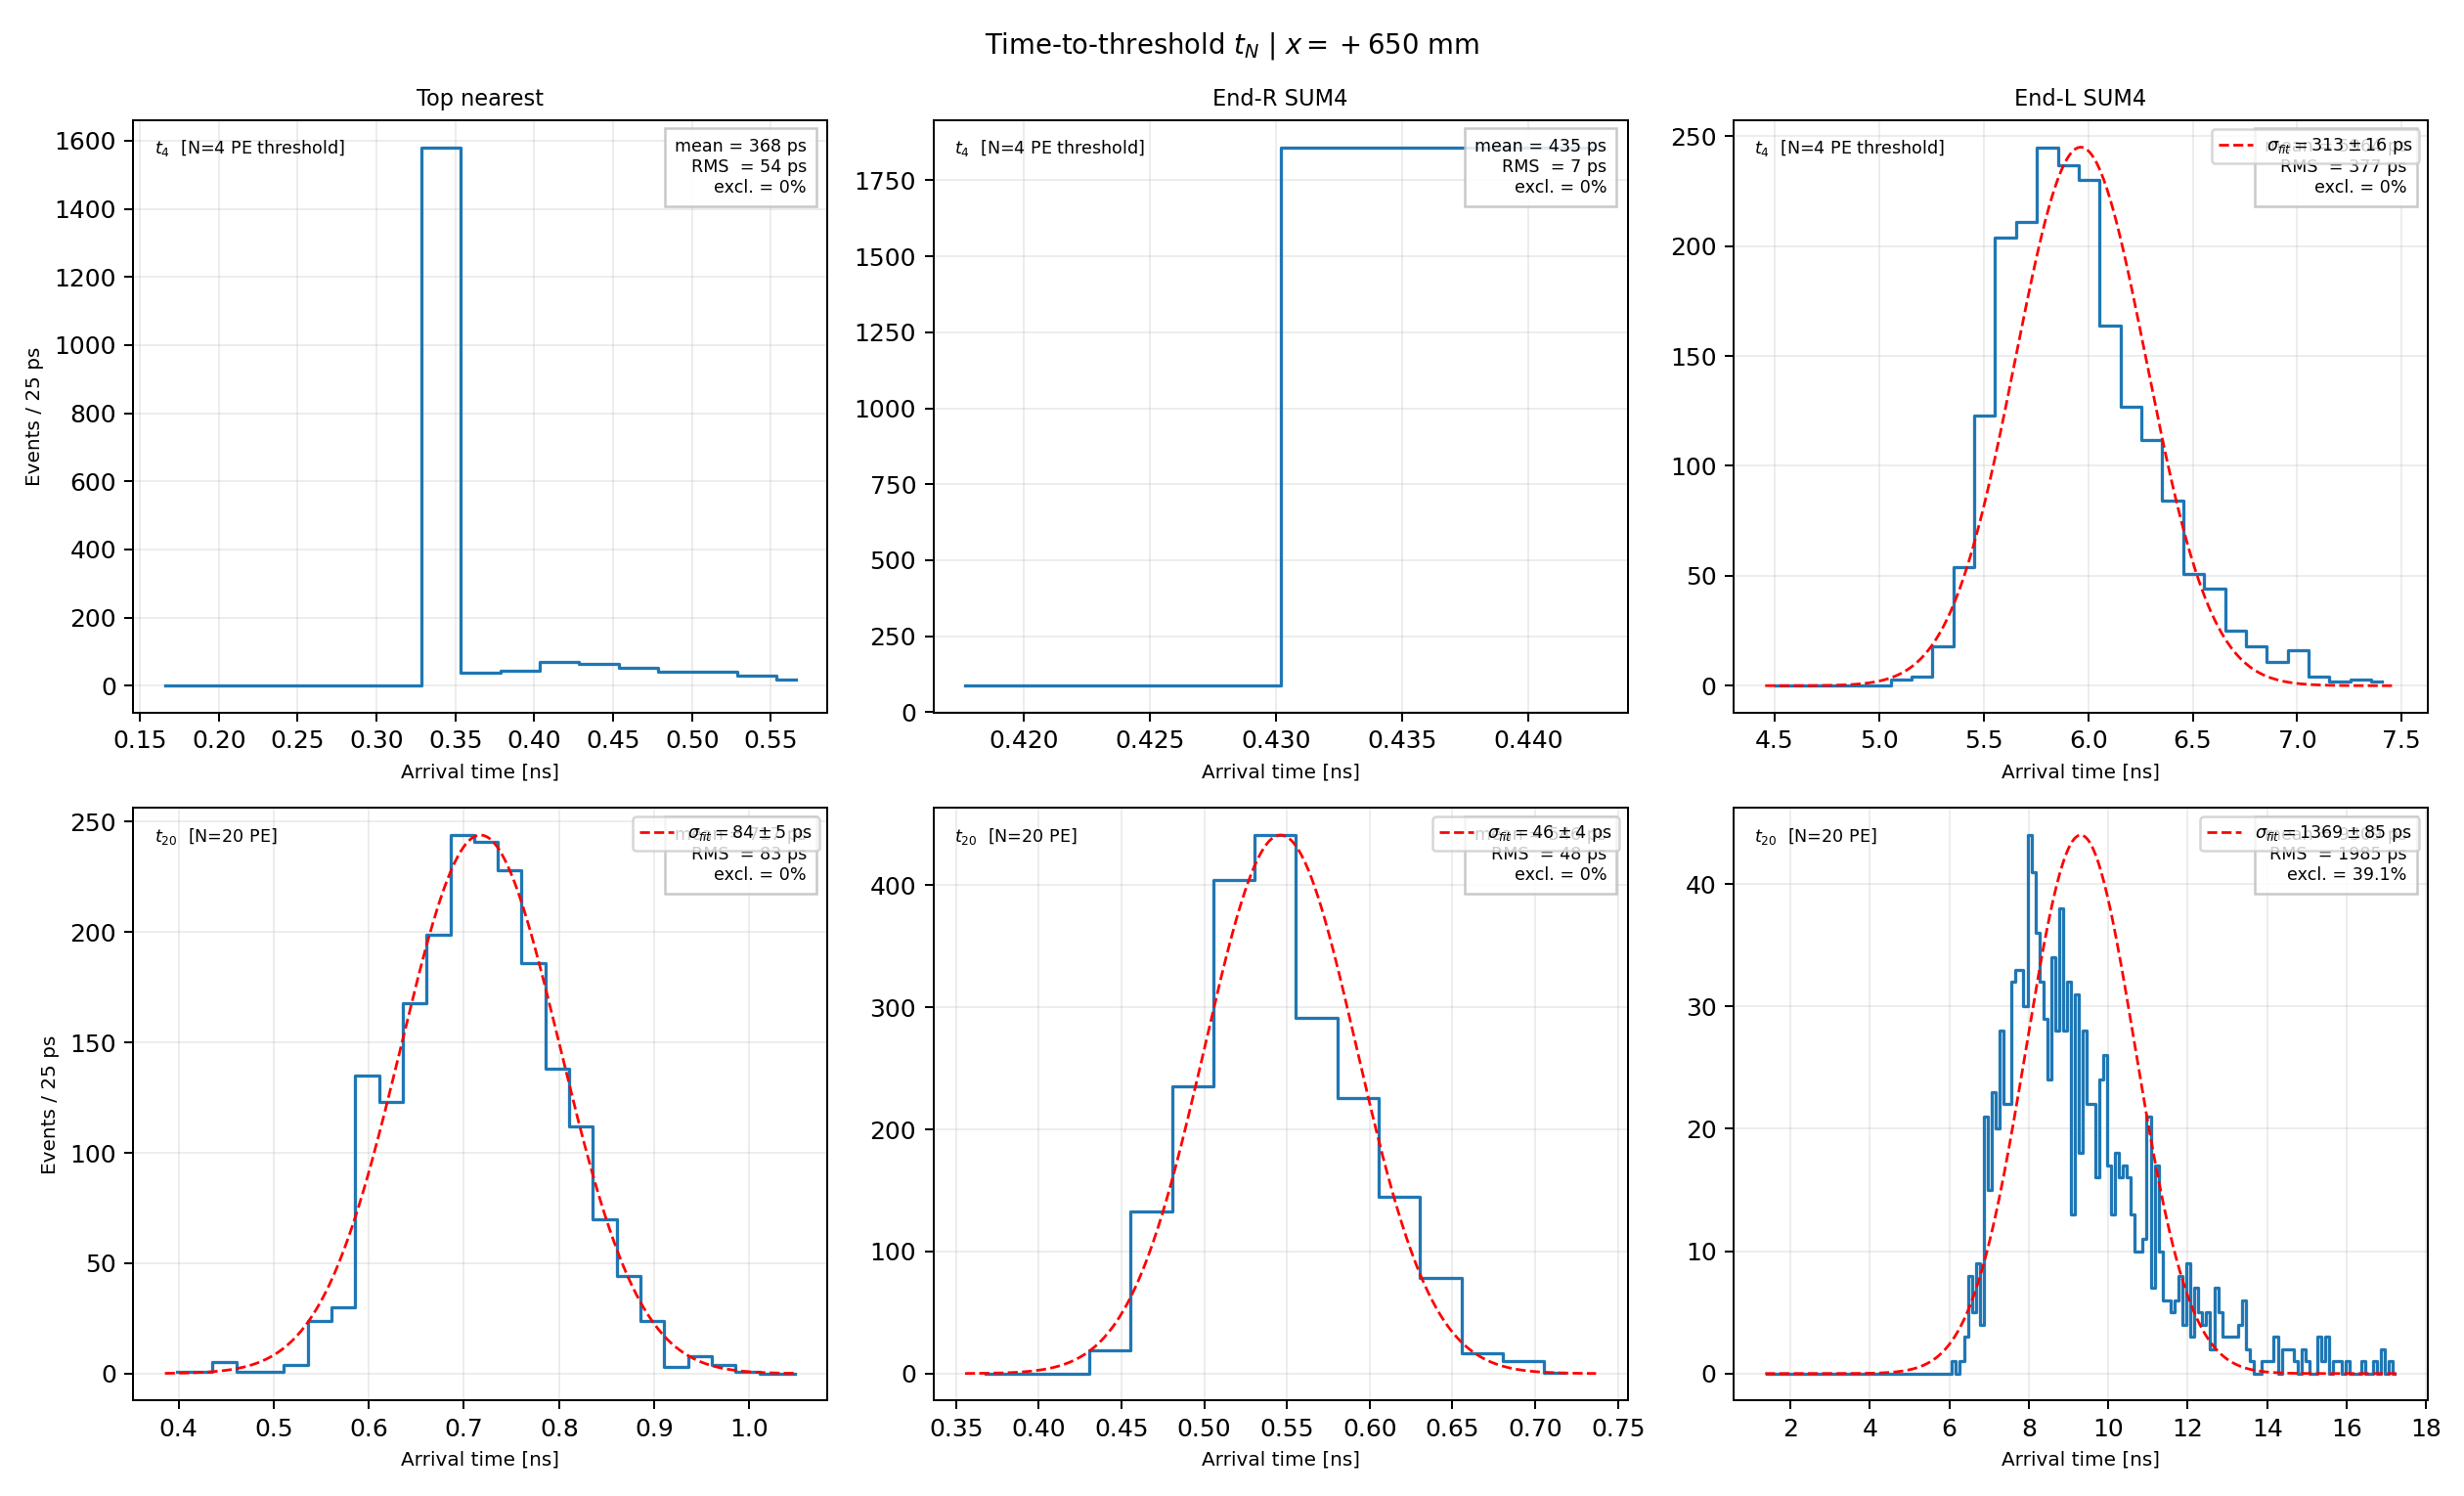
\includegraphics[width=\textwidth,height=0.84\textheight,keepaspectratio]{figs/exec12_tN_650mm.png}
\end{frame}
\begin{frame}{Position x=690 mm}

\begin{columns}[T]
  \column{0.52\textwidth}
  
\includegraphics[width=\textwidth]{figs/muon_690mm_geometry.png}
  \column{0.46\textwidth}
  
\includegraphics[width=\textwidth]{figs/muon_690mm_top_profile.png}
  \tiny
  \begin{tabular}{lr}
    \toprule Quantity & Value \\ \midrule
    End L $N_{pe}$ & $41.4\pm0.3$ \\
    End R $N_{pe}$ & $3383.2\pm18.3$ \\
    Nearest Top ID & 85 (window-track exception) \\
    Nearest Top $N_{pe}$ & $353.0\pm2.0$ \\
    Nearest Top $\langle t\rangle$ &
      $2.7881\pm0.0023$ ns \\
    Nearest Top FPT & $0.34236\pm0.00019$ ns \\
    \bottomrule
  \end{tabular}
\end{columns}

\end{frame}
\begin{frame}{Run 7 $|$ x = +690 mm $|$ Photon arrival $\langle N(t)\rangle$}
\centering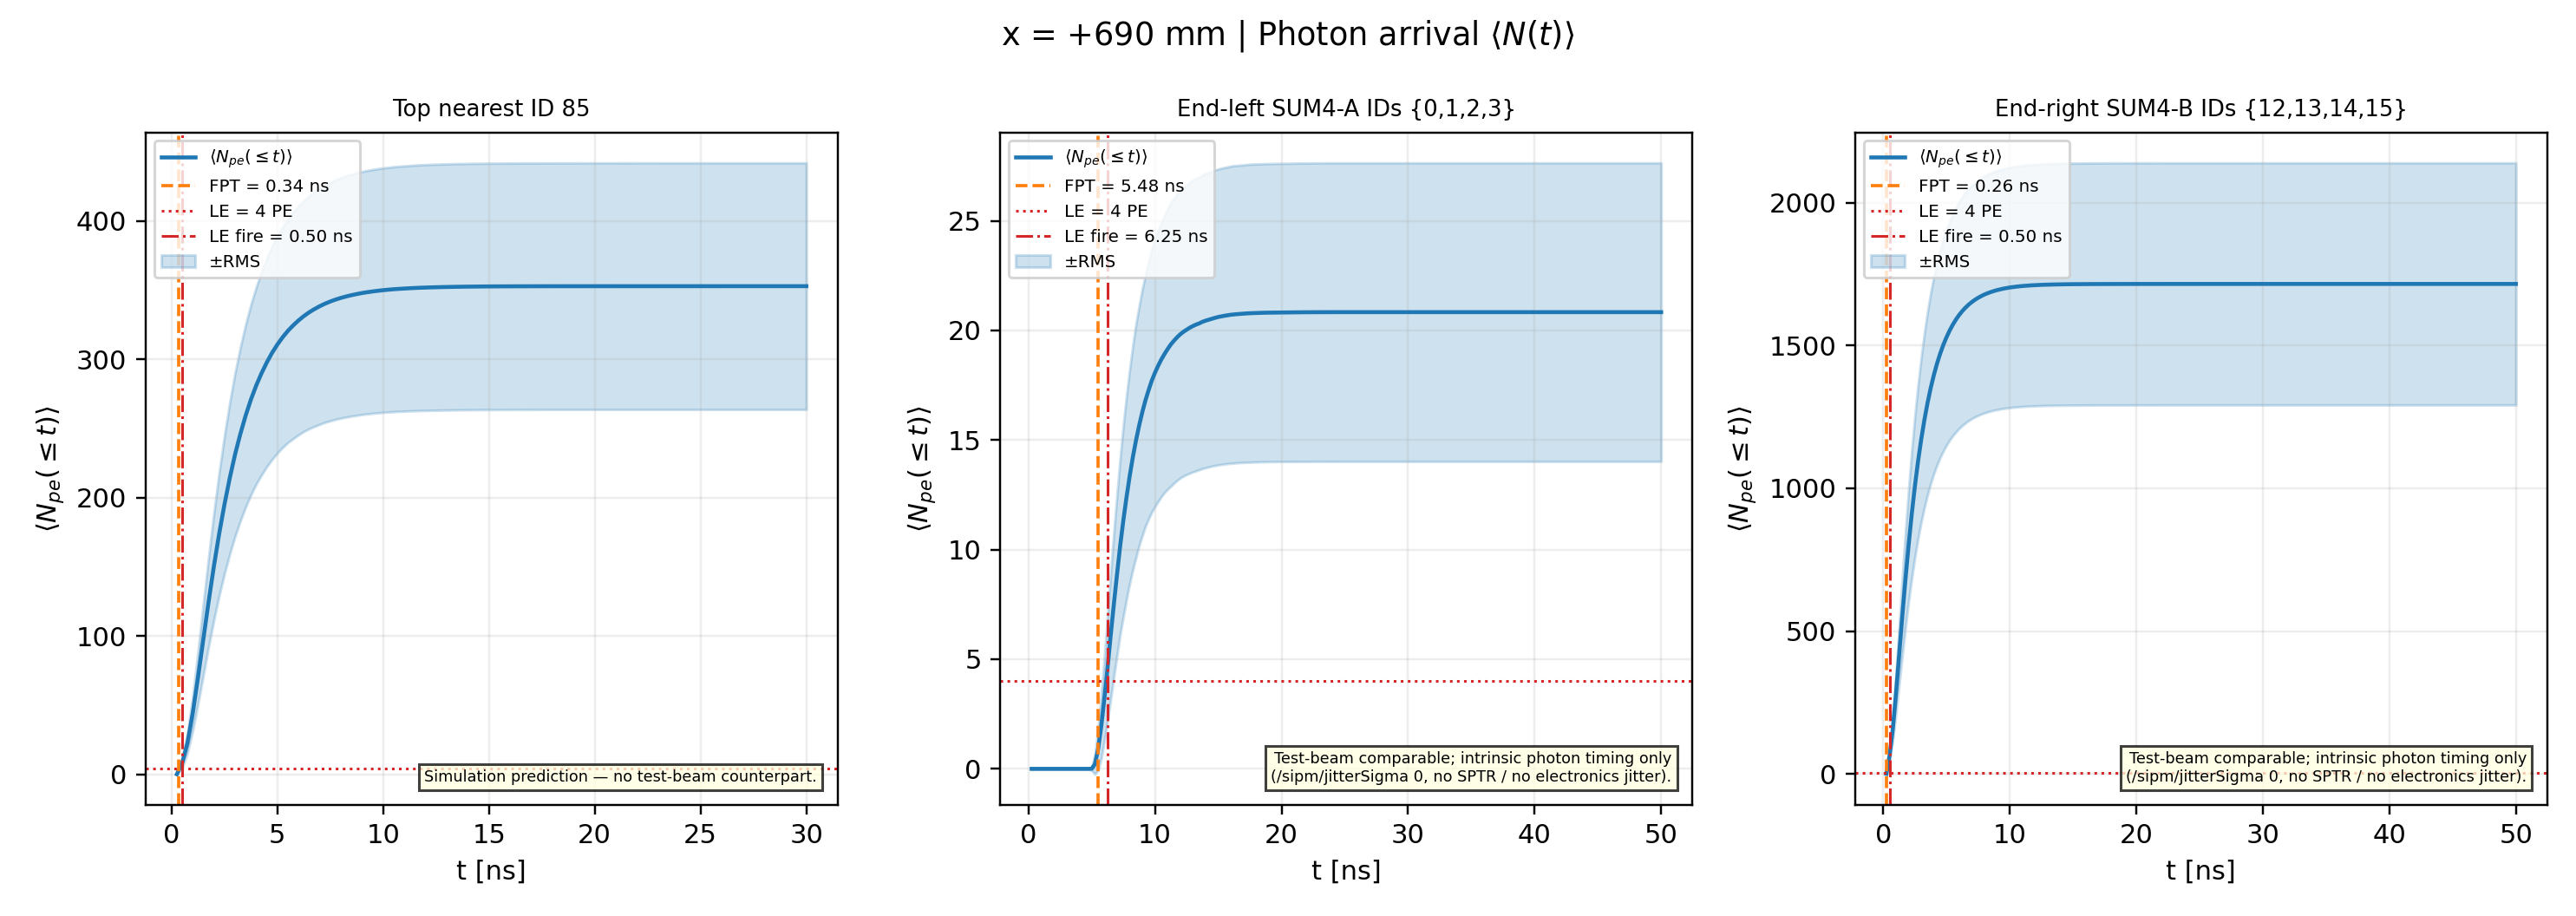
\includegraphics[width=\textwidth,height=0.78\textheight,keepaspectratio]{figs/exec11_arrival_690mm.png}
\end{frame}
\begin{frame}{Run 7 $|$ x = +690 mm $|$ Time-to-threshold $t_N$}
\centering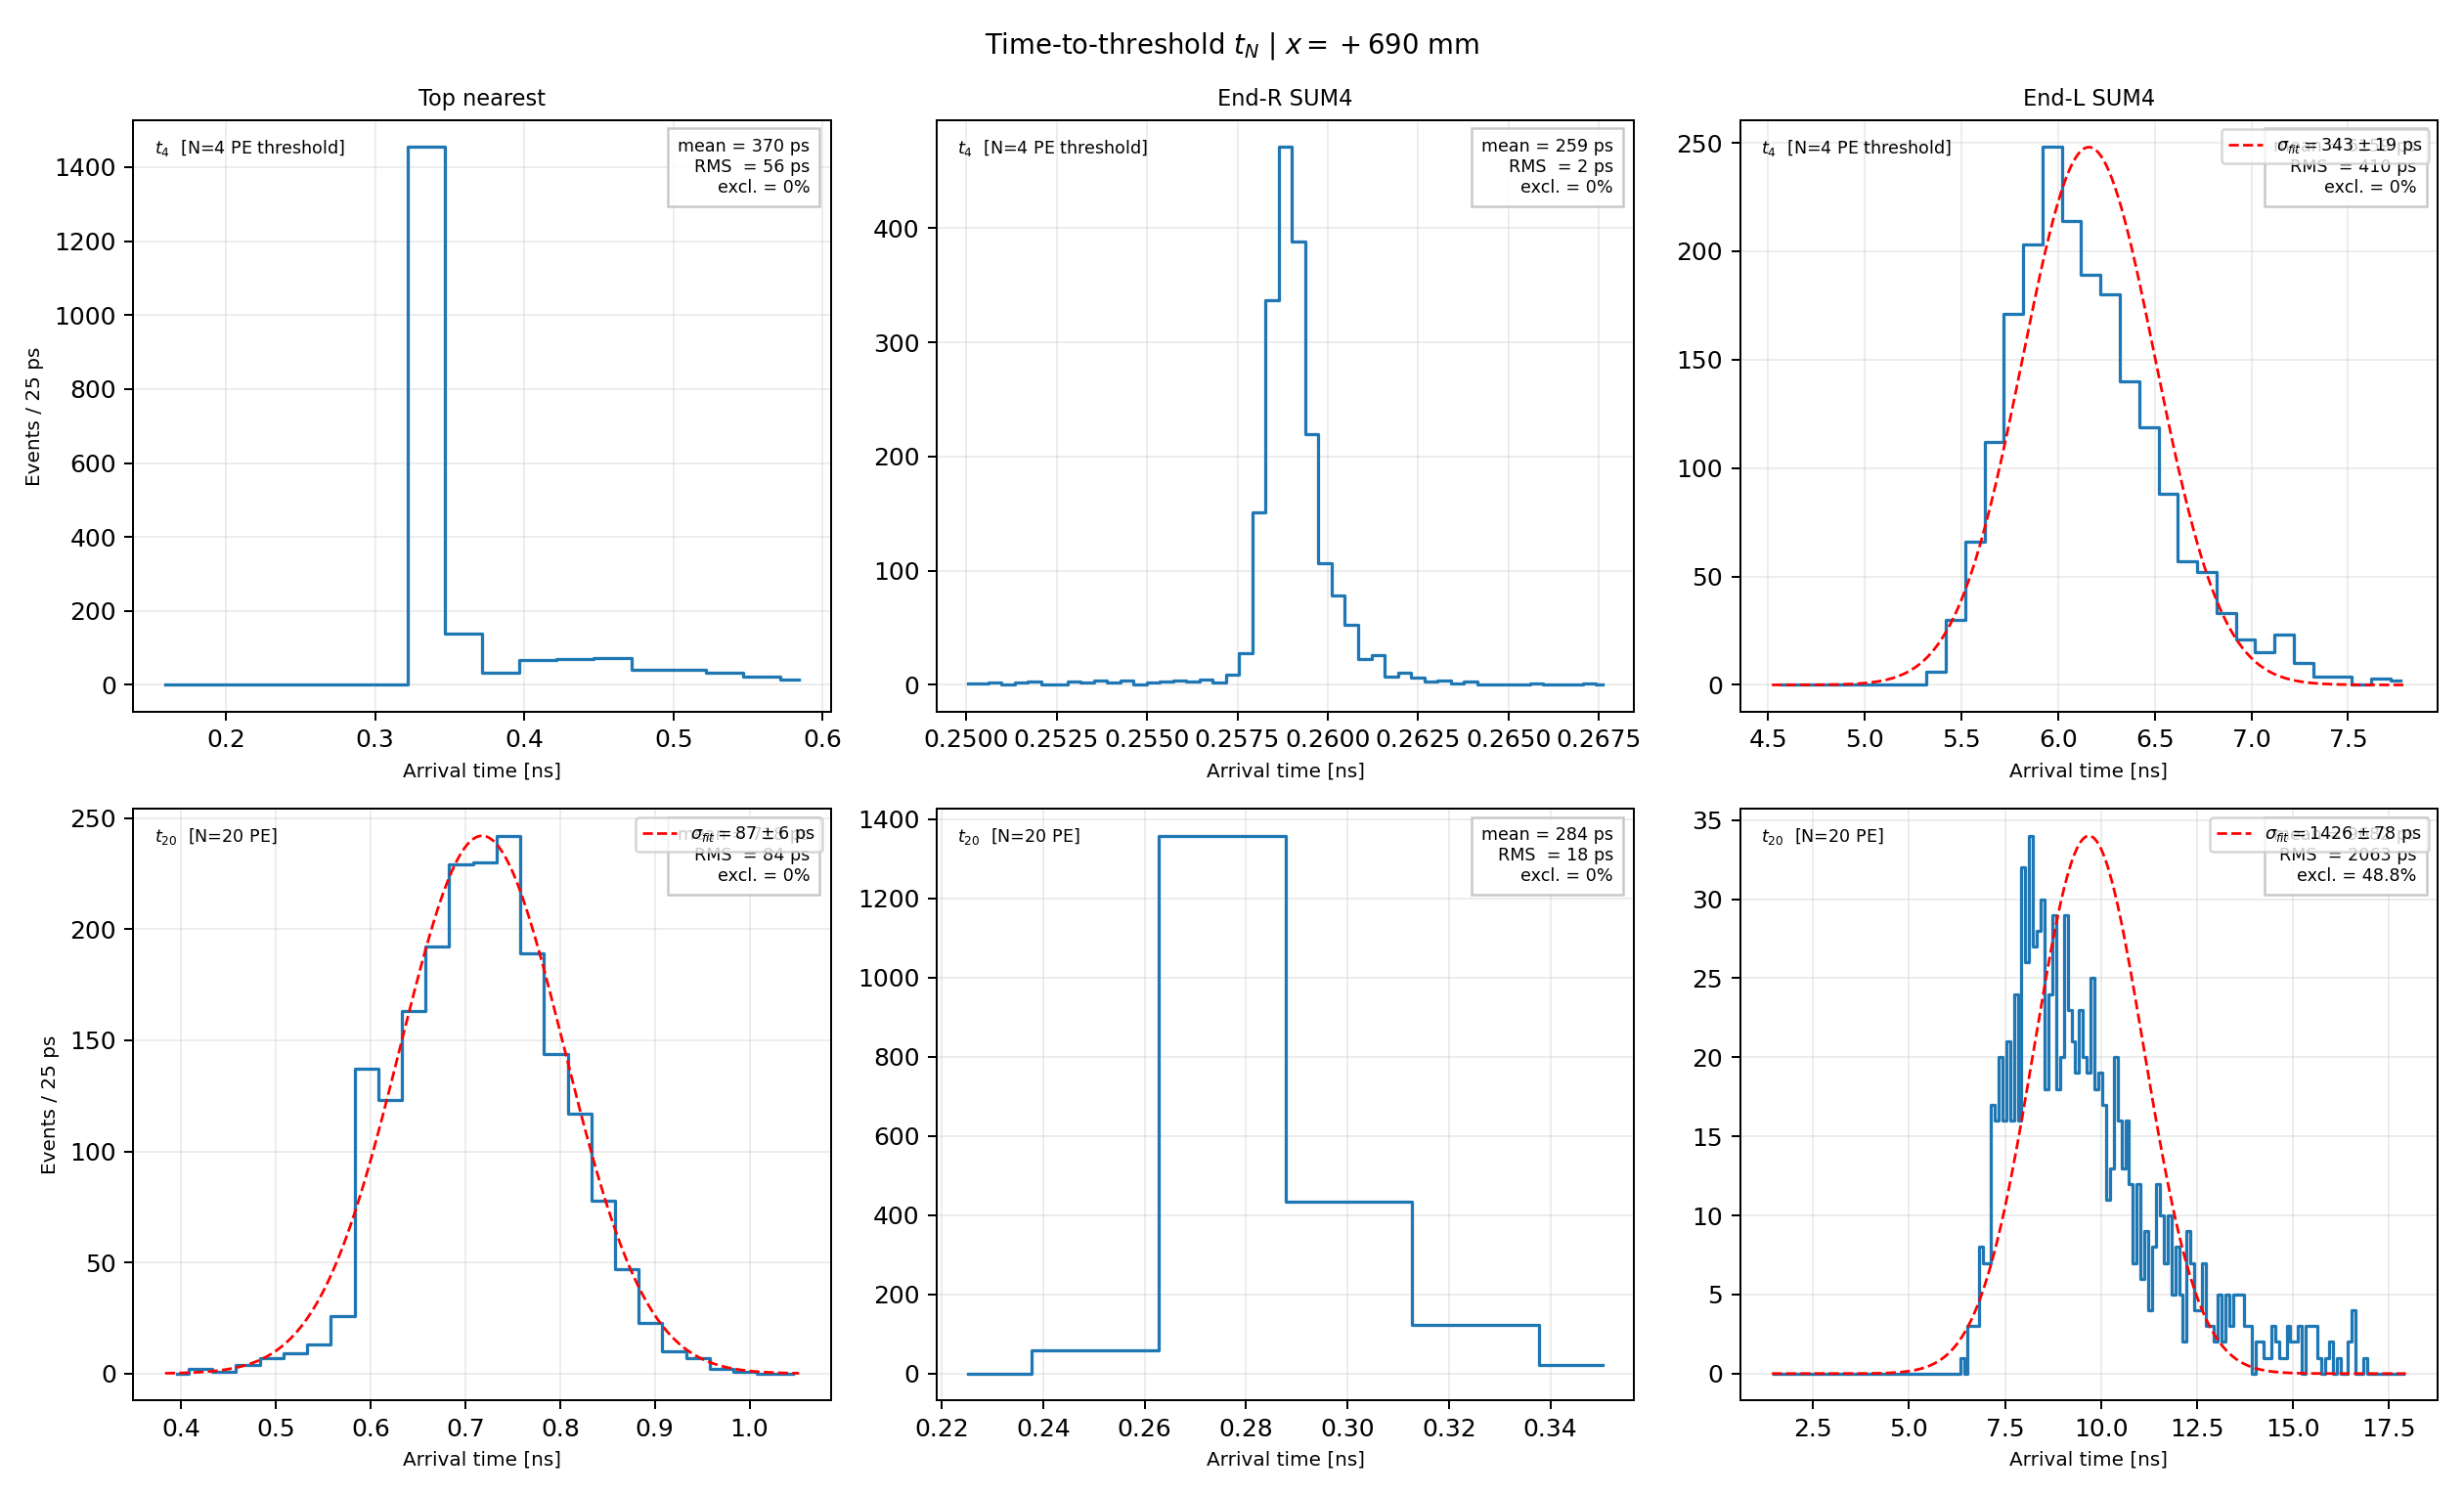
\includegraphics[width=\textwidth,height=0.84\textheight,keepaspectratio]{figs/exec12_tN_690mm.png}
\end{frame}
\begin{frame}{$\sigma(t_N)$ vs beam position: synthesis}

\centering\includegraphics[width=\textwidth,height=0.65\textheight,keepaspectratio]%
{figs/exec12_tN_summary.png}
\begin{block}{\footnotesize Interpretation and connection to $\sigma_{\rm group}$}
\scriptsize
$\sigma(t_N)$ is the single-side timing resolution at an ideal digital threshold of
$N$ detected PE; it connects the cumulative $\langle N(t)\rangle$ curves to the
published $\sigma_{\rm group}$ values.
At high $N_{pe}$ (x=$\pm690,\pm650,\pm400$ near their respective End),
$\sigma(t_4)\sim15$ ps is the pure photon-counting limit;
$\sigma_{\rm group}\sim50$ ps is larger because the analog SUM4 discriminator
adds jitter from the SPE pulse convolution ($\tau_r=0.7$ ns).
At $x=0$ (moderate $N_{pe}$, both Ends equidistant), photon-counting noise dominates
and both converge to $\sim120$ ps.
\end{block}

\end{frame}
\section{Photon budget and statistics}
\begin{frame}{Photon budget versus beam position}
\centering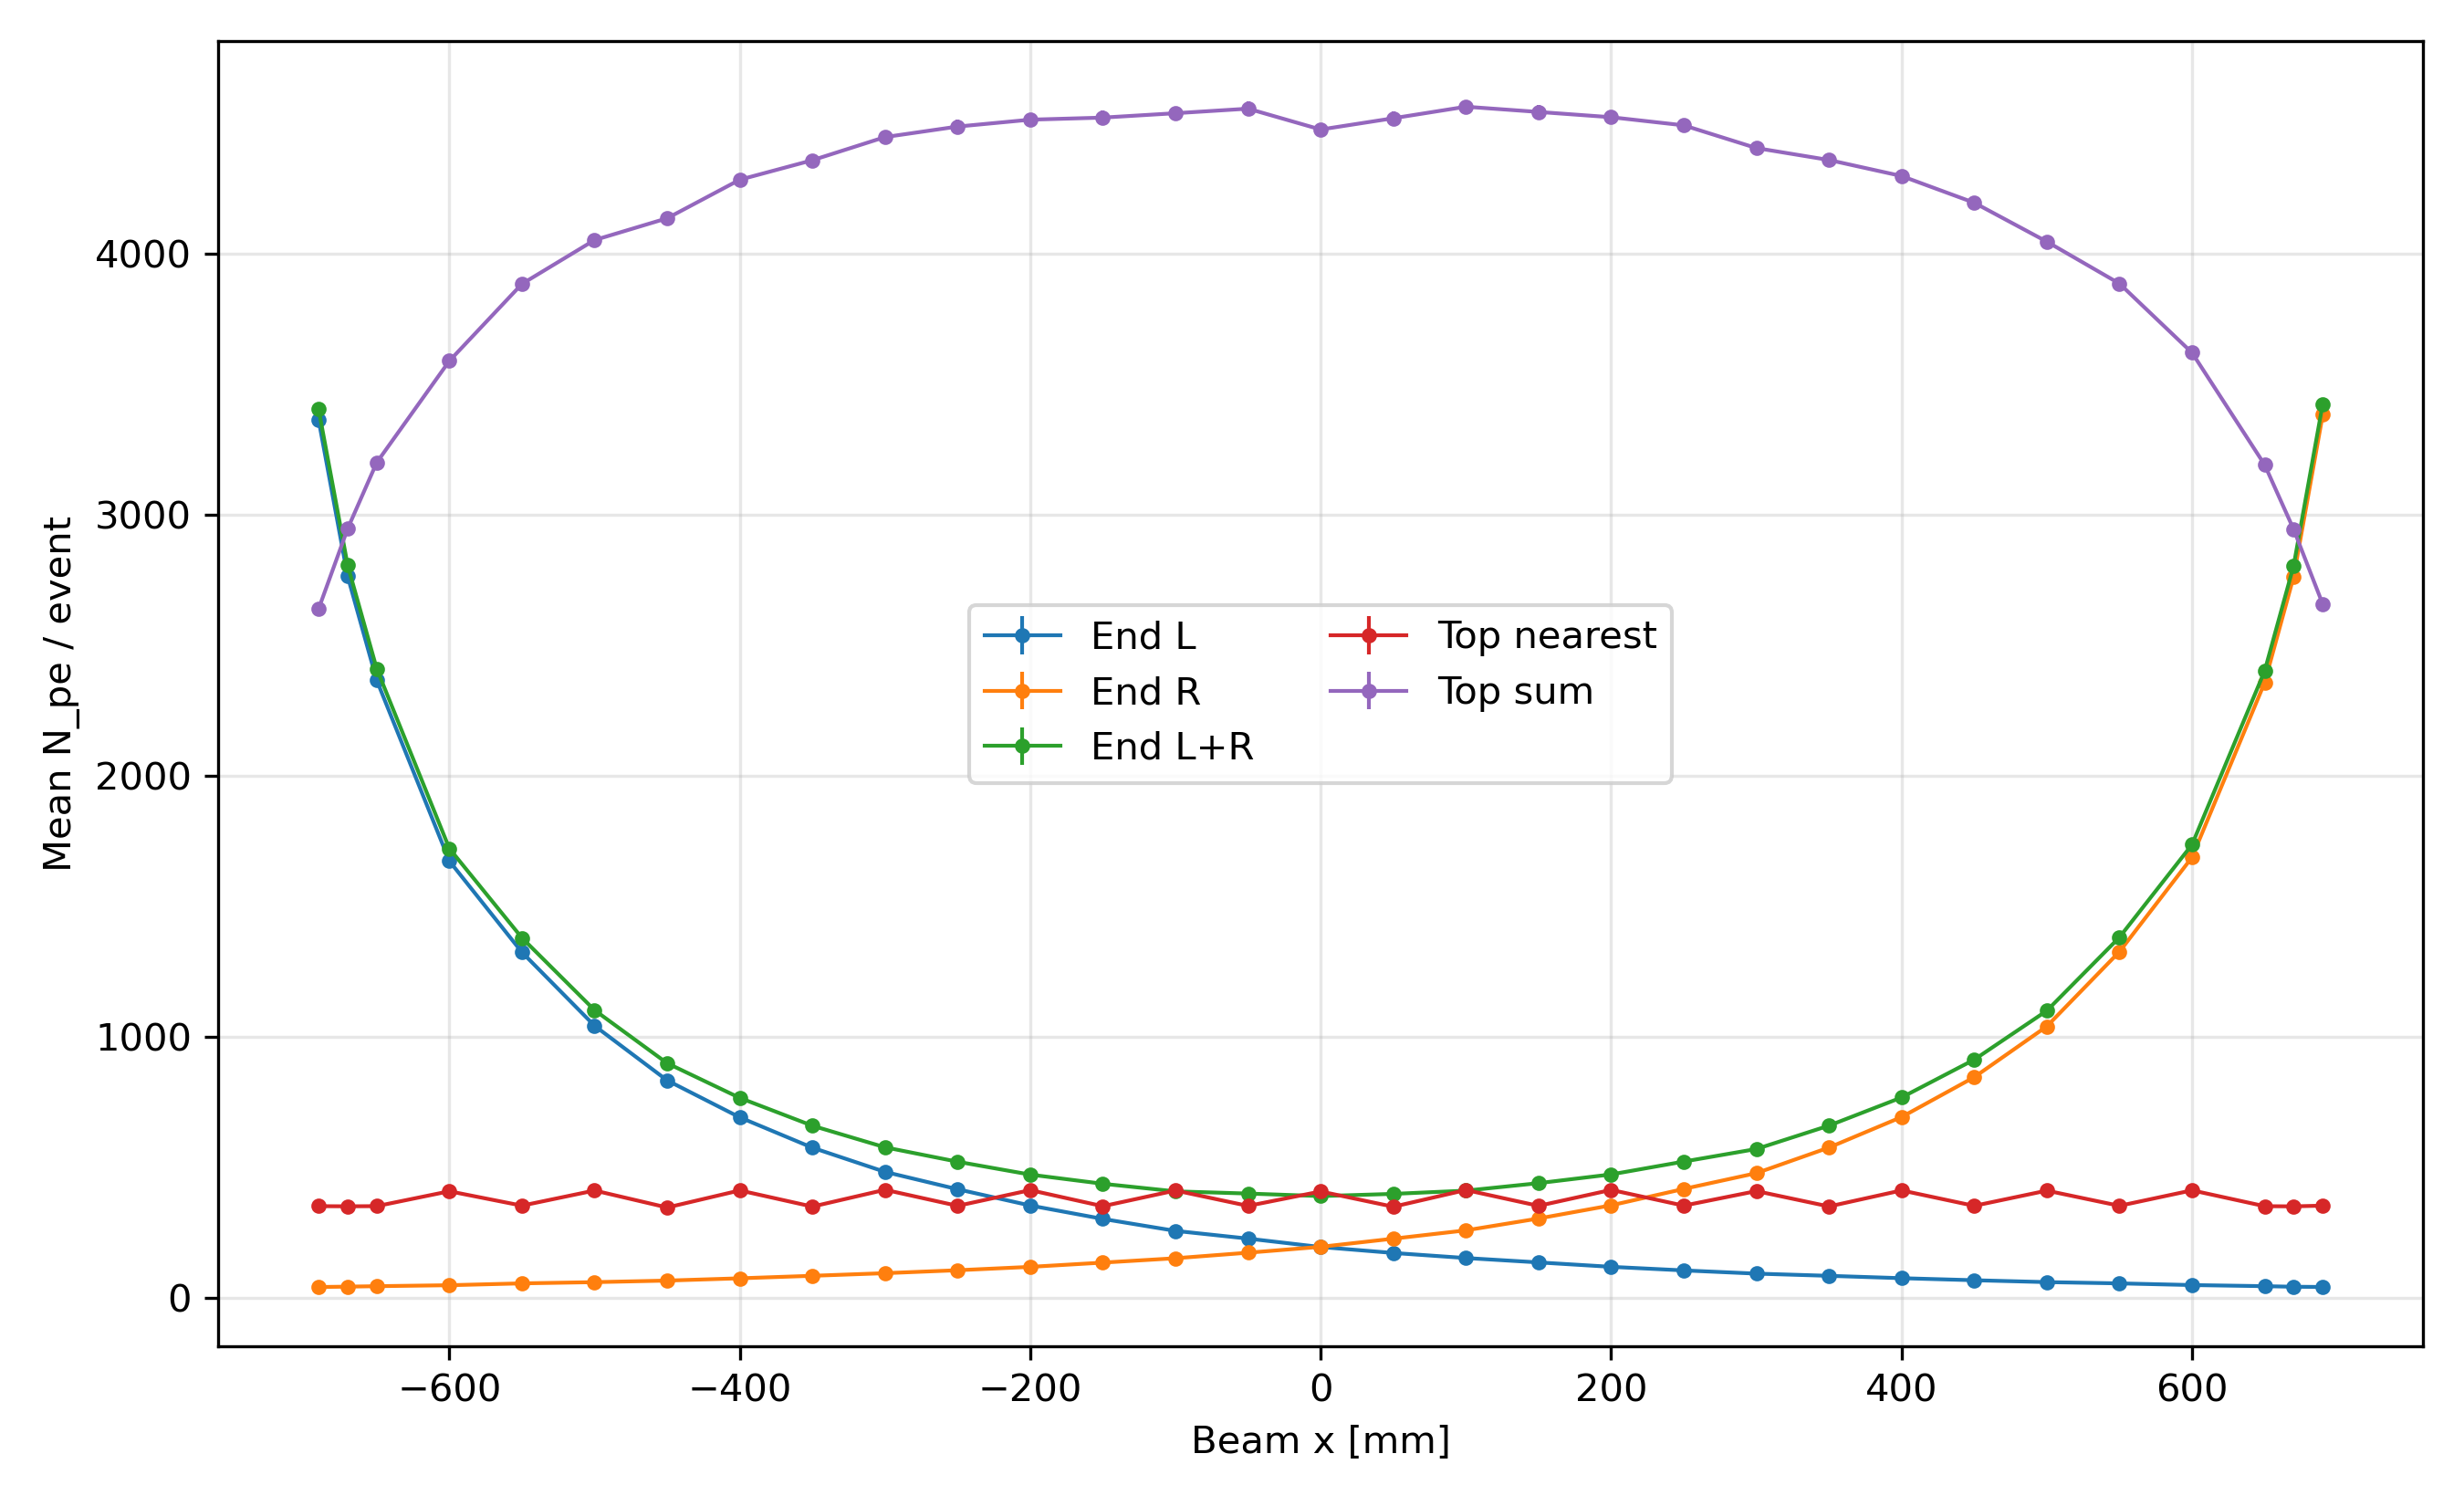
\includegraphics[width=\textwidth,height=0.62\textheight,keepaspectratio]{figs/P1_npe_vs_x.png}\begin{block}{\footnotesize How to read this plot}
\scriptsize\textbf{Why:}~Quantify $N_{pe}$ collected at each End and nearest-Top channel as the muon track scans the bar.
\par\textbf{Axes:}~x: beam position [mm]; y: mean $N_{pe}$ per event (End sums left/right and nearest Top).
\par\textbf{Takeaway:}~$N_{pe}$ decreases exponentially with track-to-End distance ($\lambda_{eff}\approx33$ cm $\ll$ ABSLENGTH $=160$ cm, system effective length); nearest-Top $N_{pe}$ peaks directly under the SiPM window.
\end{block}

\end{frame}
\begin{frame}{Top localization: full coverage diagonal}
\centering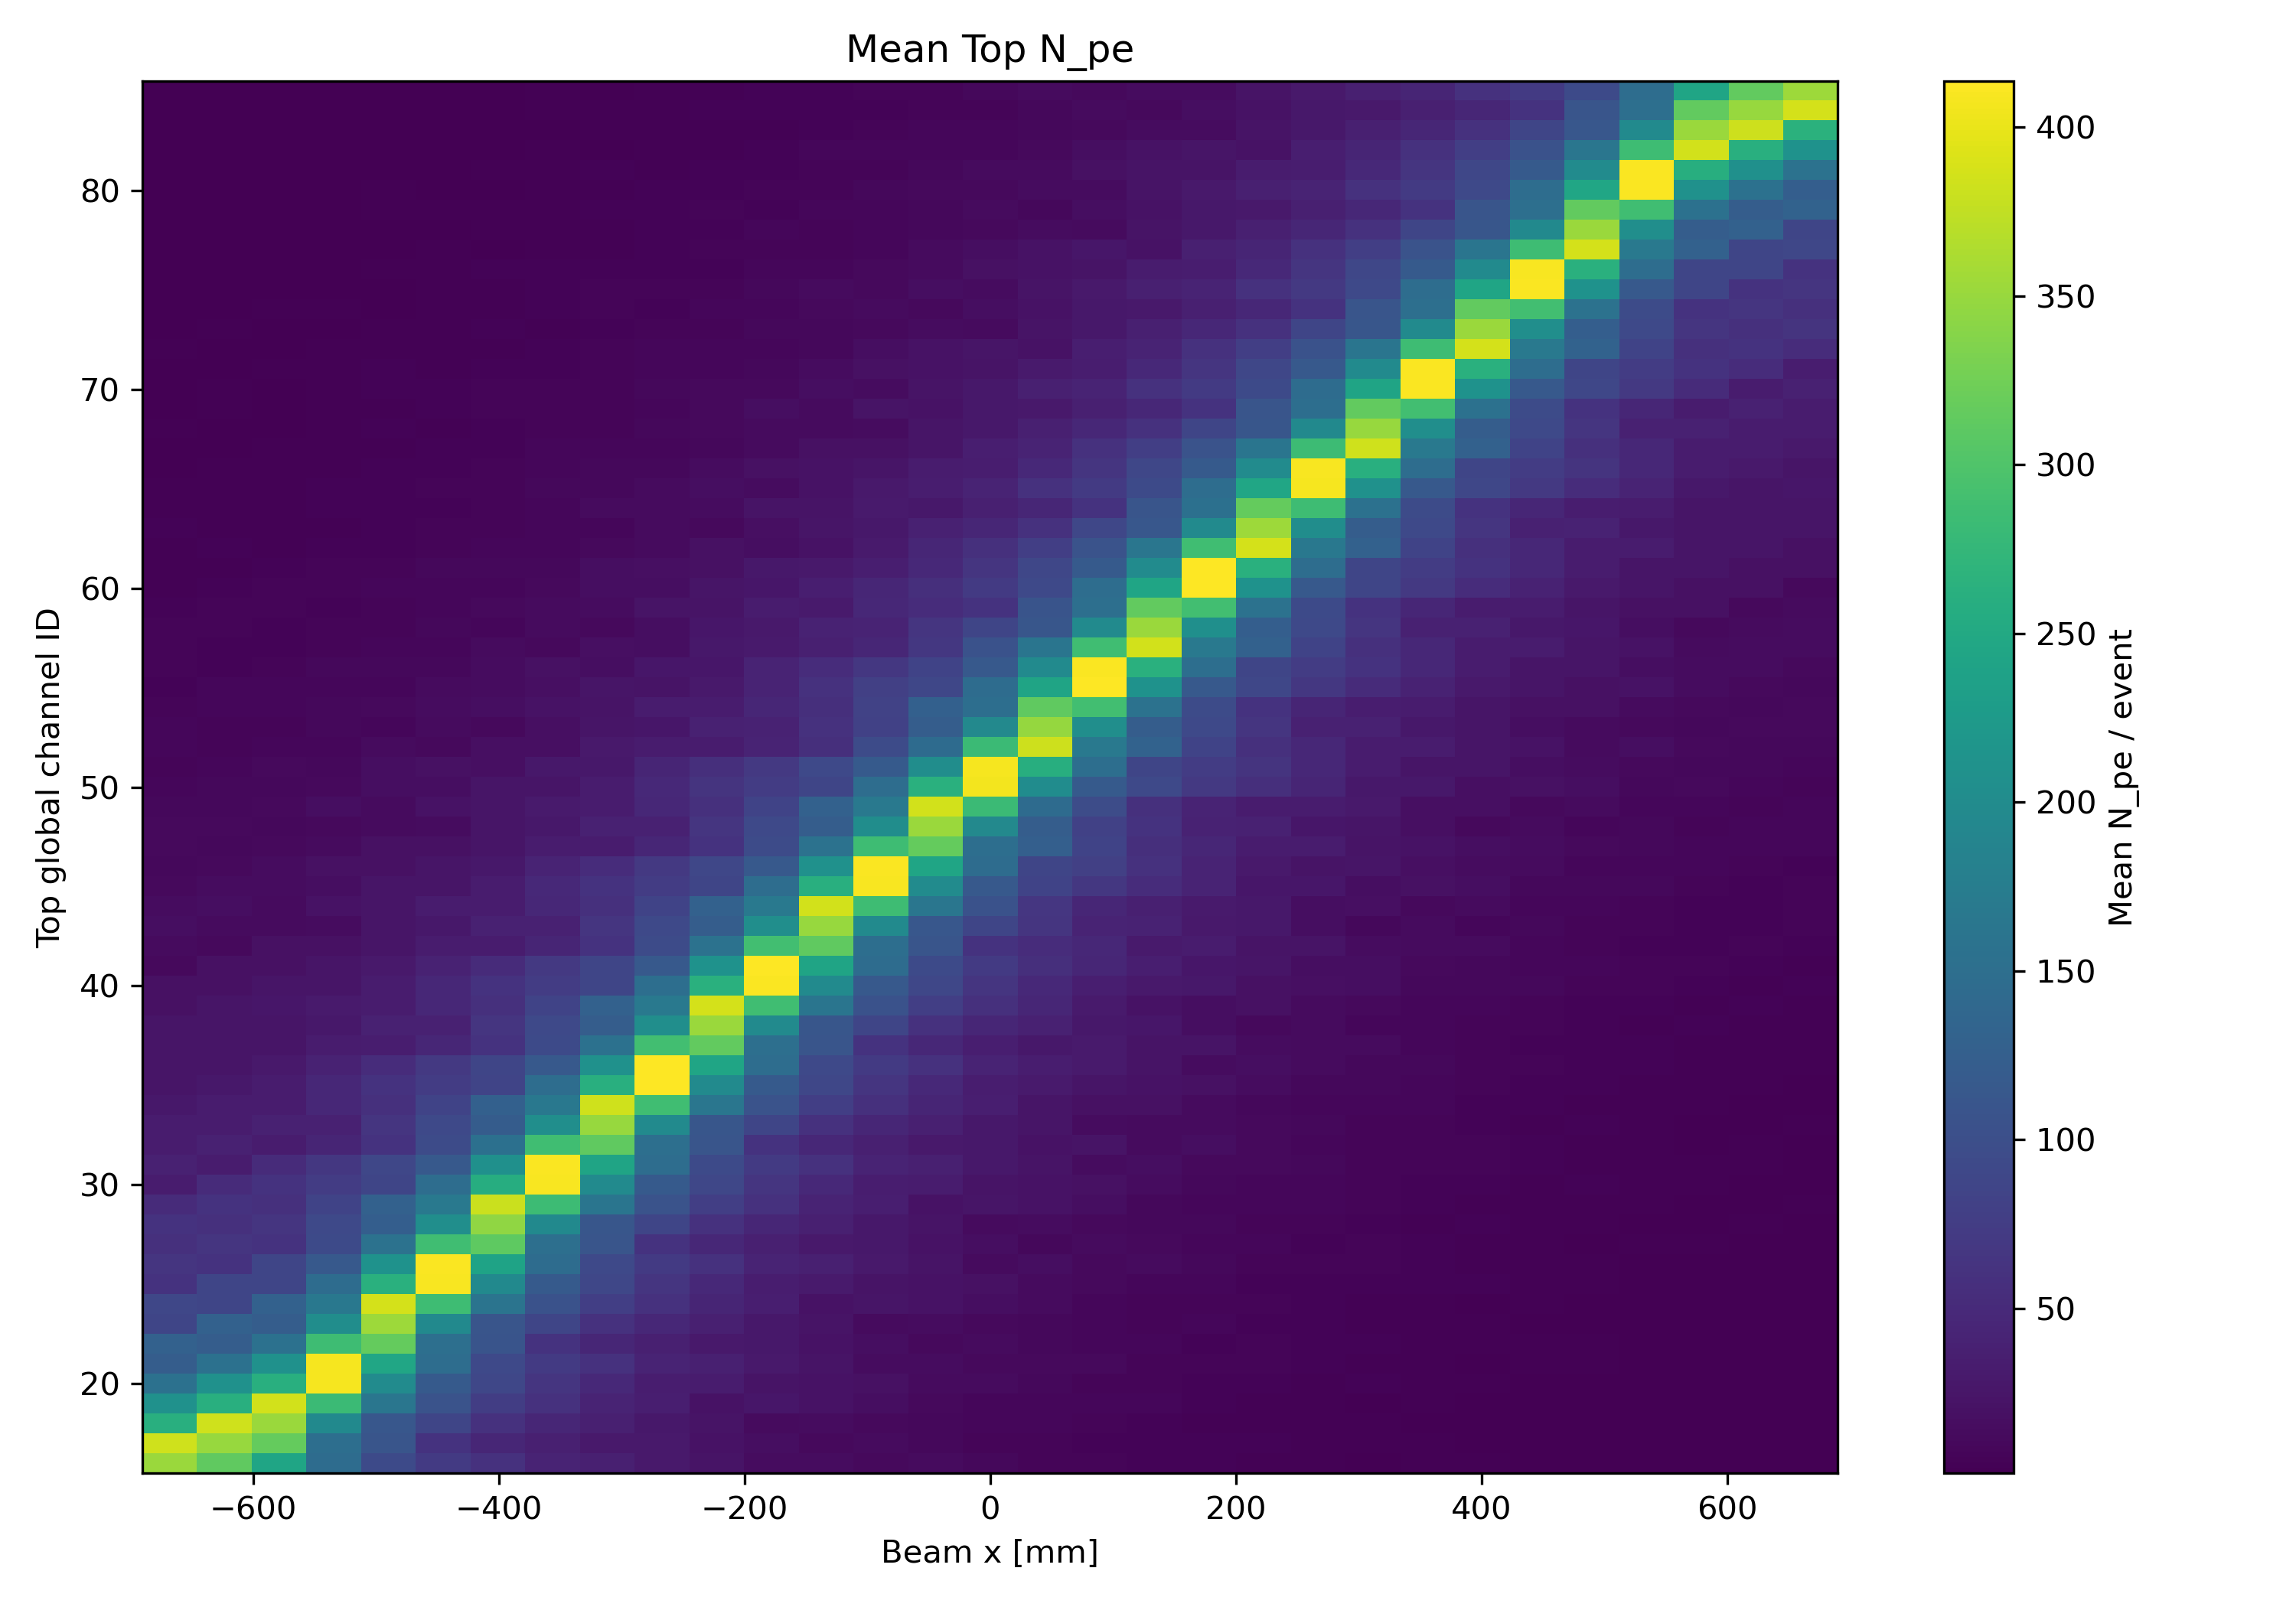
\includegraphics[width=\textwidth,height=0.62\textheight,keepaspectratio]{figs/P2_npe_heatmap_top.png}\begin{block}{\footnotesize How to read this plot}
\scriptsize\textbf{Why:}~Verify that the highest-$N_{pe}$ Top channel is always the geometrically nearest one across all 31 positions.
\par\textbf{Axes:}~x: beam position [mm]; y: Top channel ID; colour: mean $N_{pe}$.
\par\textbf{Takeaway:}~Strict diagonal coverage; window-track exception positions ($x\equiv10\pmod{20}$ mm) are labelled and pass the $<15$\% deficit criterion.
\end{block}

\end{frame}
\begin{frame}{Attenuation and the historical mean-time slope}
\centering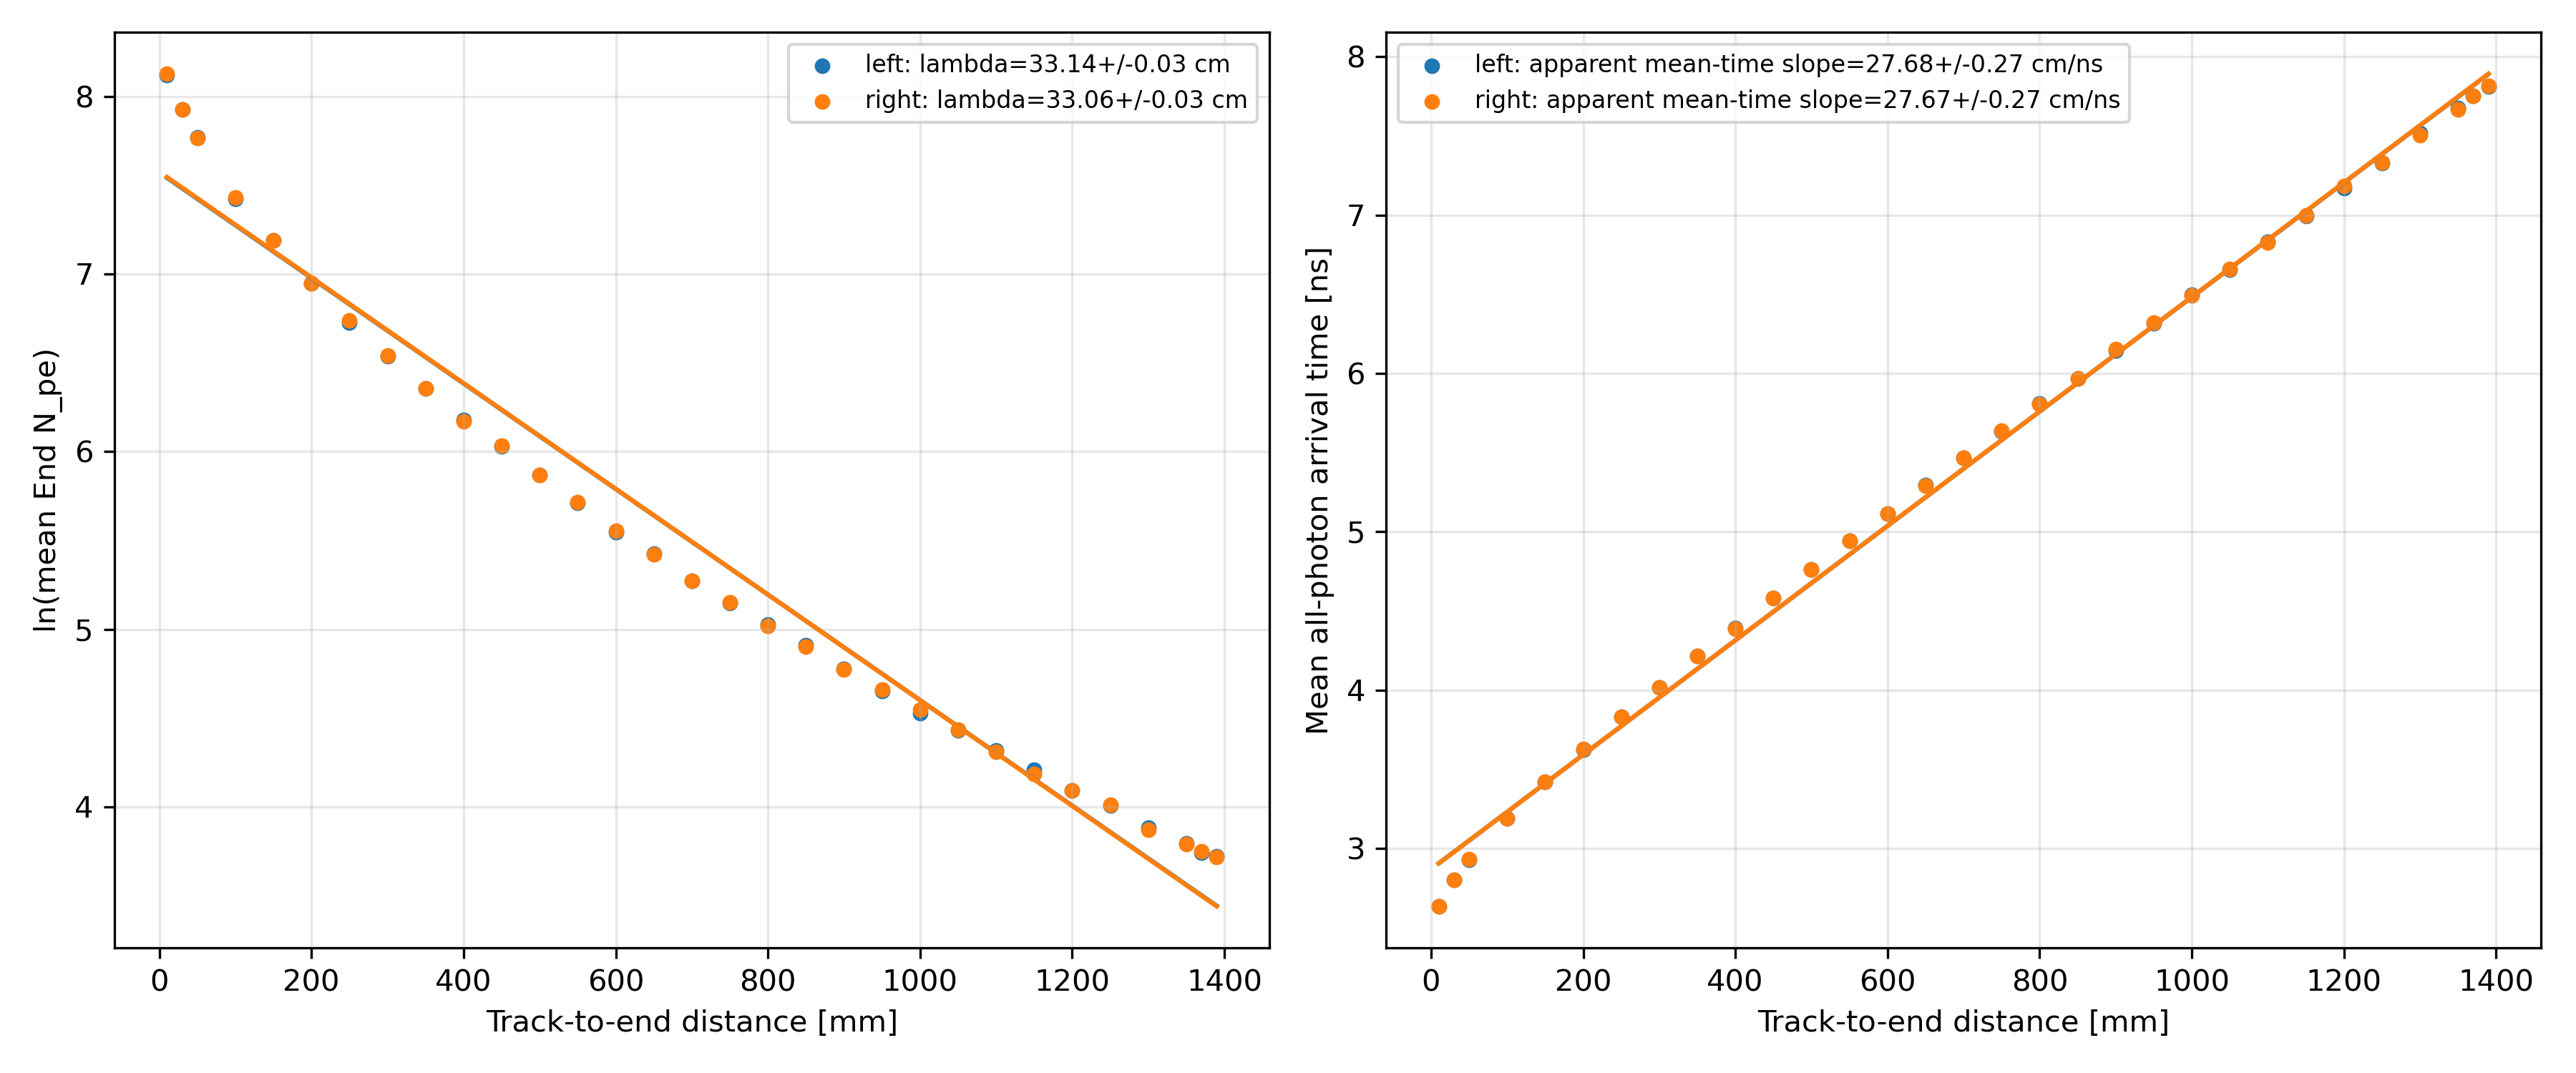
\includegraphics[width=\textwidth,height=0.55\textheight,keepaspectratio]{figs/fits_attenuation_velocity.png}\par\scriptsize $\lambda_{eff,L}=33.14\pm0.03$ cm, $\lambda_{eff,R}=33.06\pm0.03$ cm; the mean-time slope is tail-biased and is not a propagation velocity.\vspace{2pt}\begin{block}{\footnotesize How to read this plot}
\scriptsize\textbf{Why:}~Measure the effective attenuation length $\lambda_{eff}$ and test whether the mean-time slope encodes a light-propagation velocity.
\par\textbf{Axes:}~Left: mean $N_{pe}$ vs track-to-End distance [cm]; exponential fit gives $\lambda_{eff}$. Right: mean arrival time [ns] vs same distance.
\par\textbf{Takeaway:}~$\lambda_{eff}\approx33$ cm $\ll$ ABSLENGTH $=160$ cm: $\lambda_{eff}$ is a system effective length combining bulk absorption, Mylar reflection losses, and Top window drainage---not the material property. The mean-time slope is tail-biased; no propagation velocity is reliably extracted.
\end{block}

\end{frame}
\begin{frame}{Why the Fano factor grows with $\langle N_{pe}\rangle$}

\begin{columns}[T]\column{0.56\textwidth}
\begin{enumerate}\small
  \item \textbf{Pure Poisson (fixed $\Delta E$):}
        $\mathrm{Var}(N_{pe})=\langle N_{pe}\rangle$, hence $F\equiv1$.
  \item \textbf{Landau fluctuations in $\Delta E$} (law of total variance):
  \[
    \mathrm{Var}(N_{pe})=\langle N_{pe}\rangle+\!\Bigl(\tfrac{\langle N_{pe}\rangle}{\langle\Delta E\rangle}\Bigr)^{\!2}\!\mathrm{Var}(\Delta E),
  \]
  $\Rightarrow\;F=1+c\langle N_{pe}\rangle$,\enspace
  $c=\mathrm{Var}(\Delta E)/\langle\Delta E\rangle^2$
  (collection-efficiency terms absorbed in $c$).
  \item \textbf{Poisson limit $F\!\to\!1$:} only at $\langle N_{pe}\rangle\!\to\!0$
        (counting noise dominates over energy-loss fluctuations).
  \item \textbf{Effective relative fluctuation:} $\sqrt{c}\approx0.249$
        is the combined energy-loss + collection jitter,
        consistent with a thin (10 mm) plastic absorber.
\end{enumerate}
\column{0.42\textwidth}
\begin{block}{Fit result (see next slide)}
$c = 0.062162\pm0.000107$\par\medskip
The \emph{same} Landau $\Delta E$ fluctuation that shapes
the asymmetric $N_{pe}$ spectrum (next section)
also generates the super-Poissonian Fano factor:
\textbf{one physical mechanism, two observables}.
\end{block}
\end{columns}

\end{frame}
\begin{frame}{Landau dominance: Fano factor versus mean $N_{pe}$}
\centering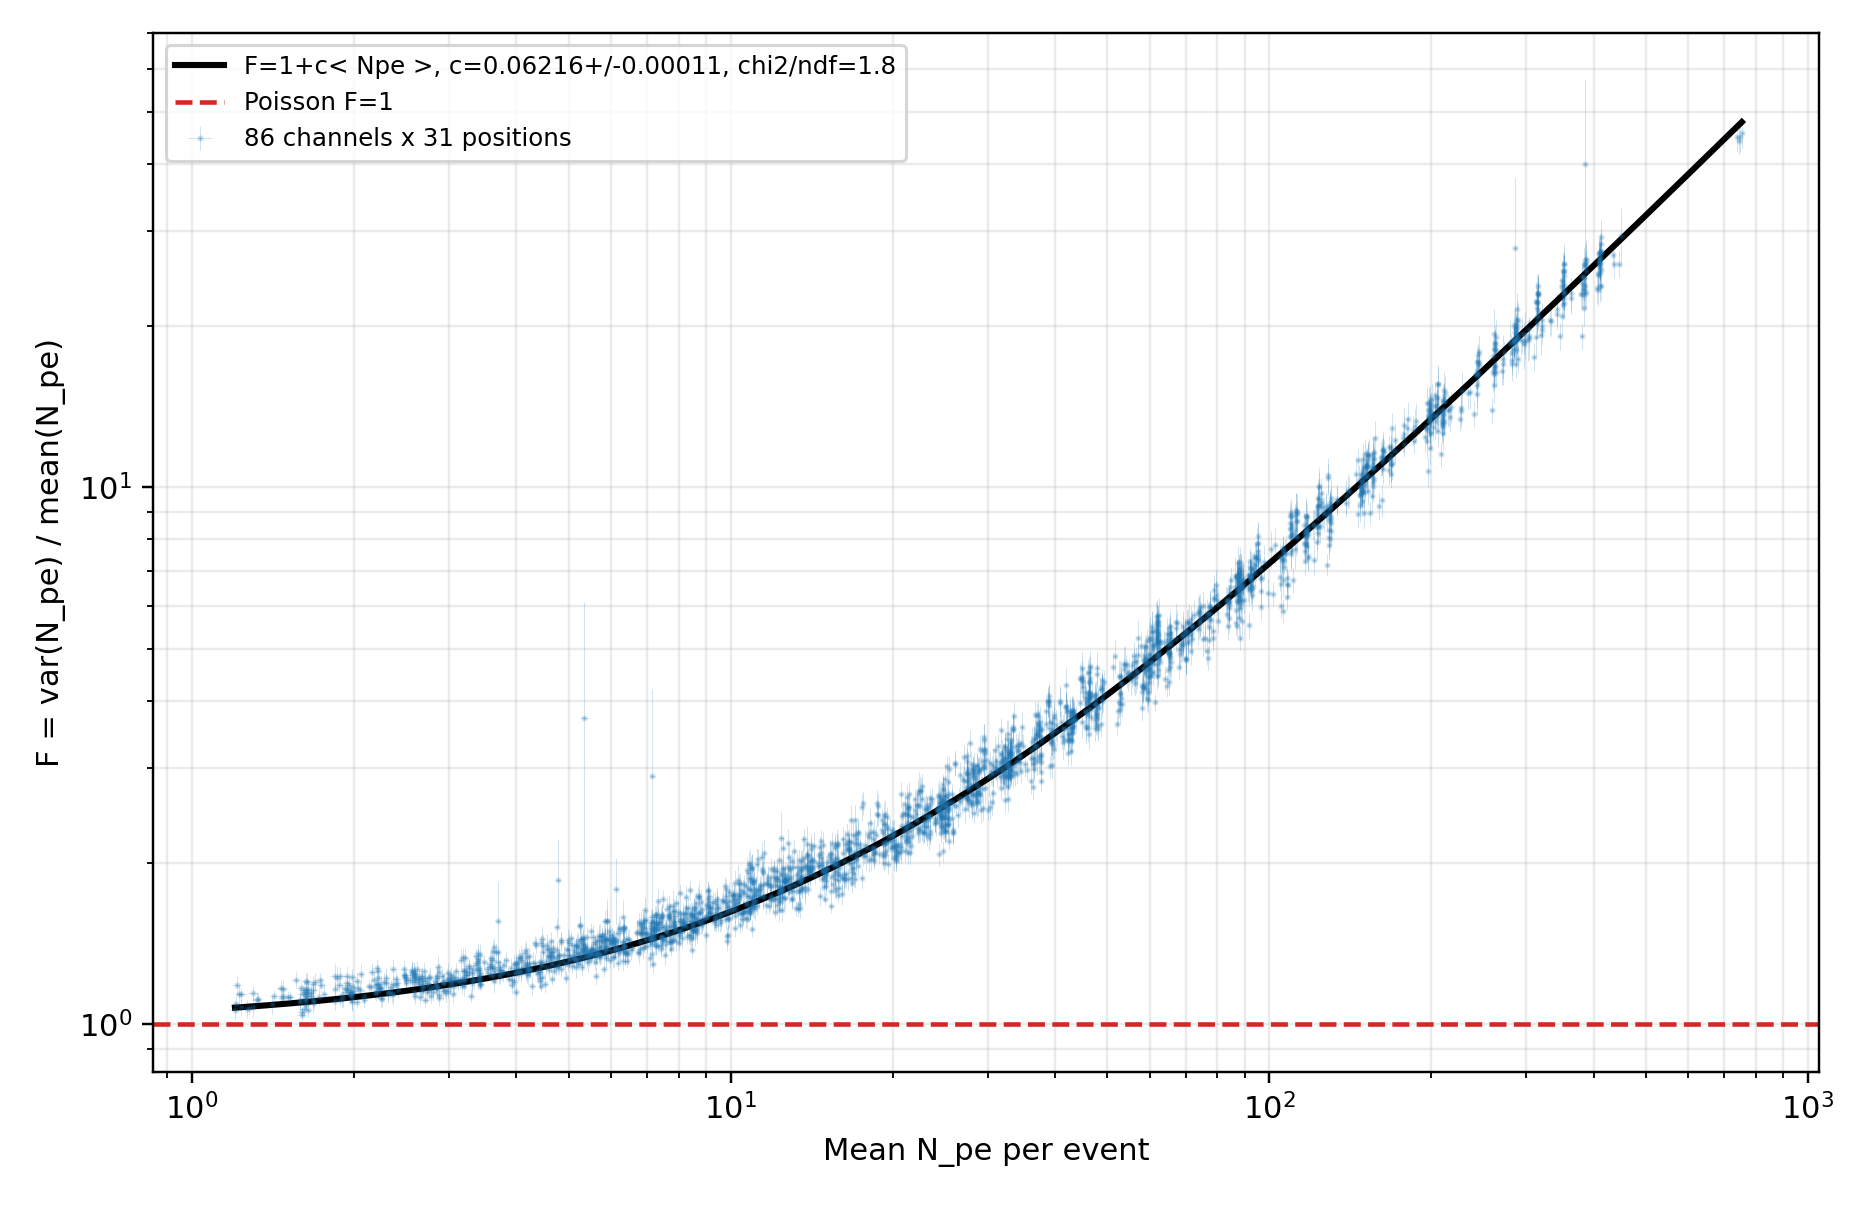
\includegraphics[width=\textwidth,height=0.55\textheight,keepaspectratio]{figs/exec10_fano_vs_mean.png}\par\scriptsize $F=1+c\langle N_{pe}\rangle$, $c=0.062162\pm0.000107$, $\chi^2/ndf=1.76$. Poisson $F=1$ is approached only at low light.\vspace{2pt}\begin{block}{\footnotesize How to read this plot}
\scriptsize\textbf{Why:}~Measure $F=\mathrm{Var}(N_{pe})/\langle N_{pe}\rangle$ to distinguish Poisson ($F=1$) from Landau-dominated fluctuations.
\par\textbf{Axes:}~x: $\langle N_{pe}\rangle$ per event; y: $\mathrm{Var}/\langle N_{pe}\rangle$. Dashed: Poisson $F=1$. Line: linear fit $F=1+c\langle N_{pe}\rangle$.
\par\textbf{Takeaway:}~$F$ grows linearly: Landau $\Delta E$ fluctuations dominate counting noise at all light levels. $\sqrt{c}$ is the effective relative energy-loss fluctuation of this 10 mm absorber.
\end{block}

\end{frame}
\begin{frame}{Why Landau (and why Moyal as analytic proxy)}

\begin{columns}[T]
\column{0.50\textwidth}
\textbf{Why not Gaussian:}\par\smallskip
\begin{itemize}\small
  \item In 10 mm of plastic the muon undergoes many collisions, but
        the energy-transfer cross-section ($\mathrm{d}\sigma/\mathrm{d}\varepsilon\propto1/\varepsilon^2$,
        Rutherford/M{\o}ller) has a hard tail.
  \item Rare large transfers ($\delta$-rays) dominate the variance;
        the variance per collision diverges and the Central Limit Theorem
        does not apply.
  \item Result: asymmetric distribution with a hard right tail ---
        the Landau distribution.
  \item Gaussian (Vavilov$\to$Gauss) limit only applies to \emph{thick} absorbers.
\end{itemize}
\column{0.48\textwidth}
\textbf{Why Moyal:}\par\smallskip
\begin{itemize}\small
  \item Landau density has no closed form (contour integral).
  \item The Moyal function is a closed-form analytic approximation
        to the Landau core and early tail, enabling stable MINUIT fits.
  \item \textit{Known limitation:} extreme Moyal tail undershoots
        true Landau tail; fit quality degrades at high $N_{pe}$.
\end{itemize}
\medskip
\textbf{Moyal $\otimes$ Gauss:}\par\smallskip
\begin{itemize}\small
  \item Photo-electron counting (Poisson) and collection fluctuations
        broaden the peak symmetrically.
  \item Full model: Moyal $\otimes$ Gaussian.
  \item Connects to Fano slide: same Landau $\Delta E$ fluctuation,
        two observables (spectrum shape + super-Poissonian $F$).
\end{itemize}
\end{columns}

\end{frame}
\begin{frame}{High-light example: Moyal--Gaussian Landau proxy}
\centering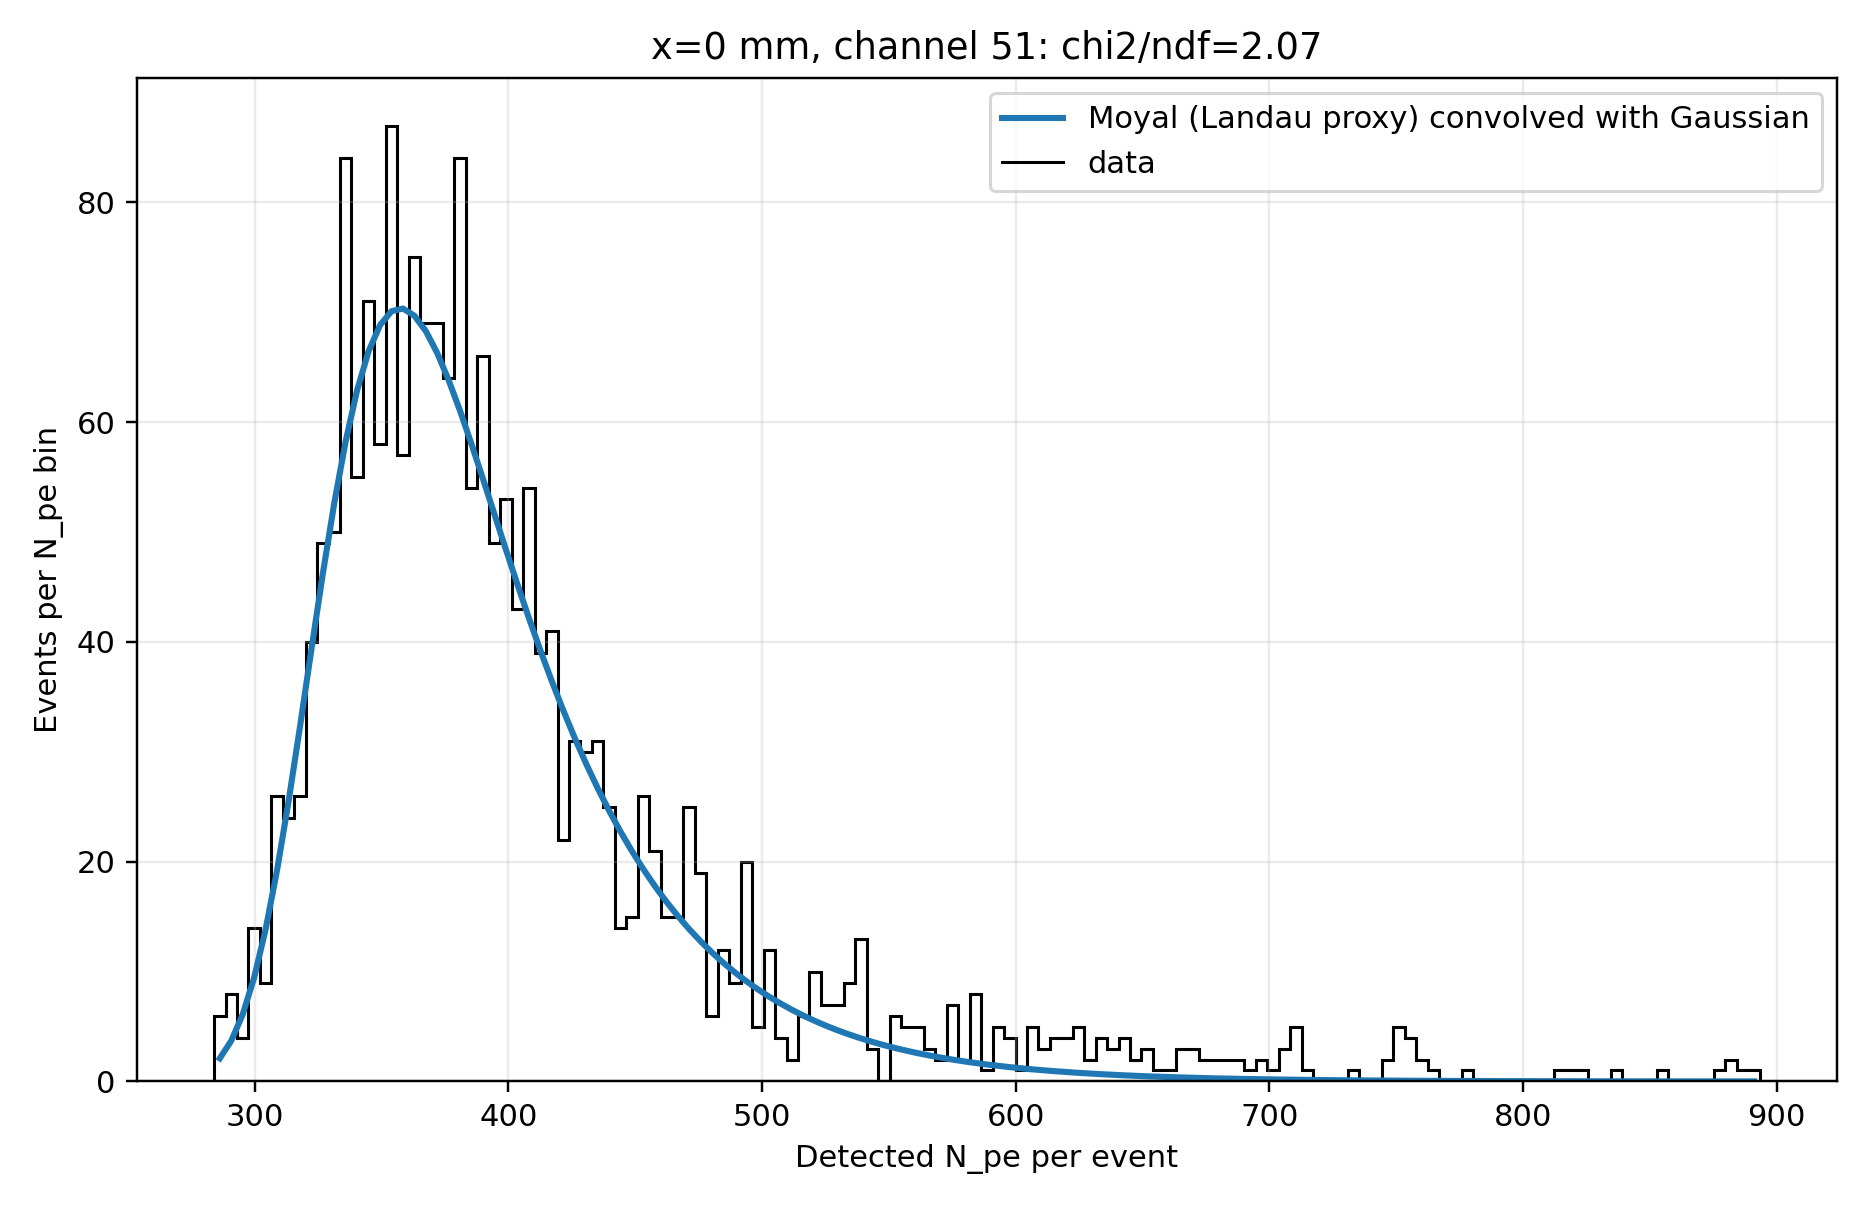
\includegraphics[width=\textwidth,height=0.55\textheight,keepaspectratio]{figs/exec10_landau_fit_example.png}\par\scriptsize Moyal approximates Landau. Some channels have poor $\chi^2$ or an unidentifiable Gaussian width; all recorded in \texttt{exec10\_landau\_mpv.csv}.\vspace{2pt}\begin{block}{\footnotesize How to read this plot}
\scriptsize\textbf{Why:}~Fit the $N_{pe}$ spectrum at a high-yield position to quantify the Landau MPV and width.
\par\textbf{Axes:}~x: $N_{pe}$ per event; y: counts. Data (step), Moyal$\otimes$Gauss fit (curve).
\par\textbf{Takeaway:}~Core described by Moyal proxy; hard right tail from $\delta$-rays. MPVs are future inputs for test-beam ToT calibration.
\end{block}

\end{frame}
\begin{frame}{Arrival-time examples: absolute rate and normalized shape}
\centering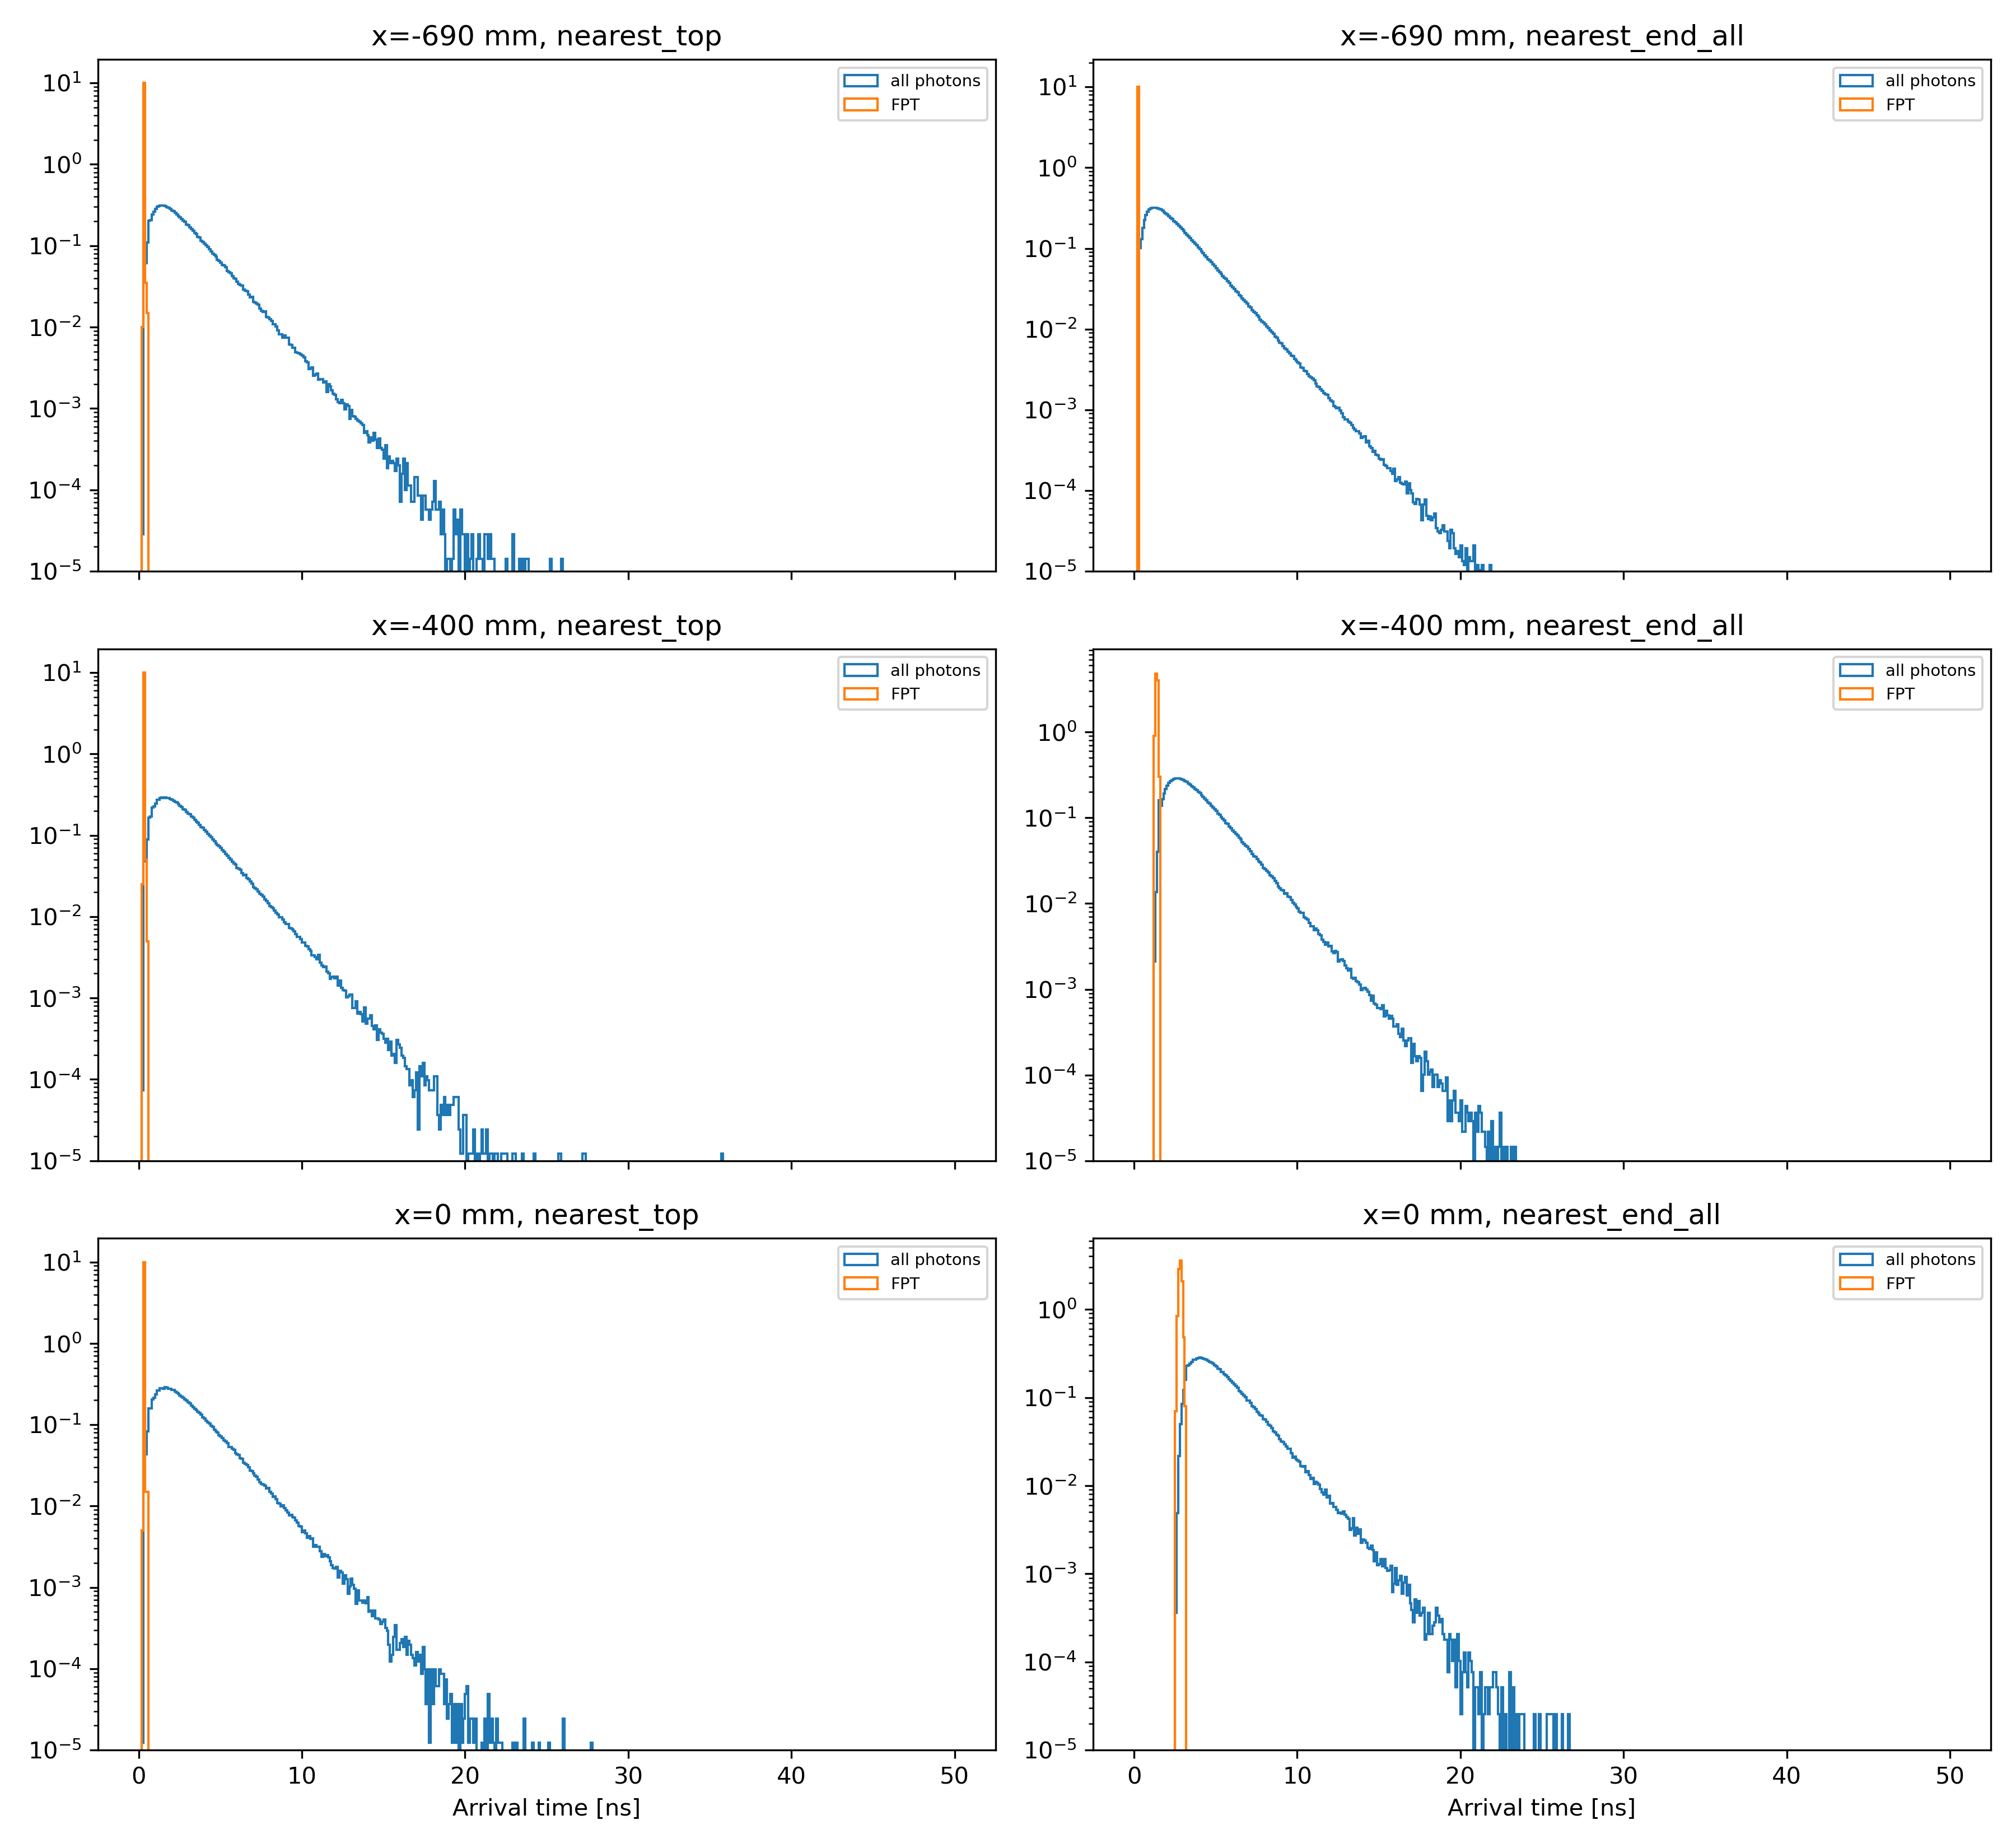
\includegraphics[width=\textwidth,height=0.55\textheight,keepaspectratio]{figs/P5_tdist_examples.png}\par\scriptsize Left: entries per event per ns. Right: area-normalized distributions. FPT = first detected photon time per event.\vspace{2pt}\begin{block}{\footnotesize How to read this plot}
\scriptsize\textbf{Why:}~Illustrate the arrival-time structure of individual Top channels and contrast absolute rate vs shape.
\par\textbf{Axes:}~x: arrival time [ns]; y: left is entries/event/ns, right is area-normalized density [1/ns].
\par\textbf{Takeaway:}~FPT distribution captures the prompt scintillation leading edge; the broad tail reflects multiple-reflection photons.
\end{block}

\end{frame}
\begin{frame}{Mean arrival time and FPT versus x}
\centering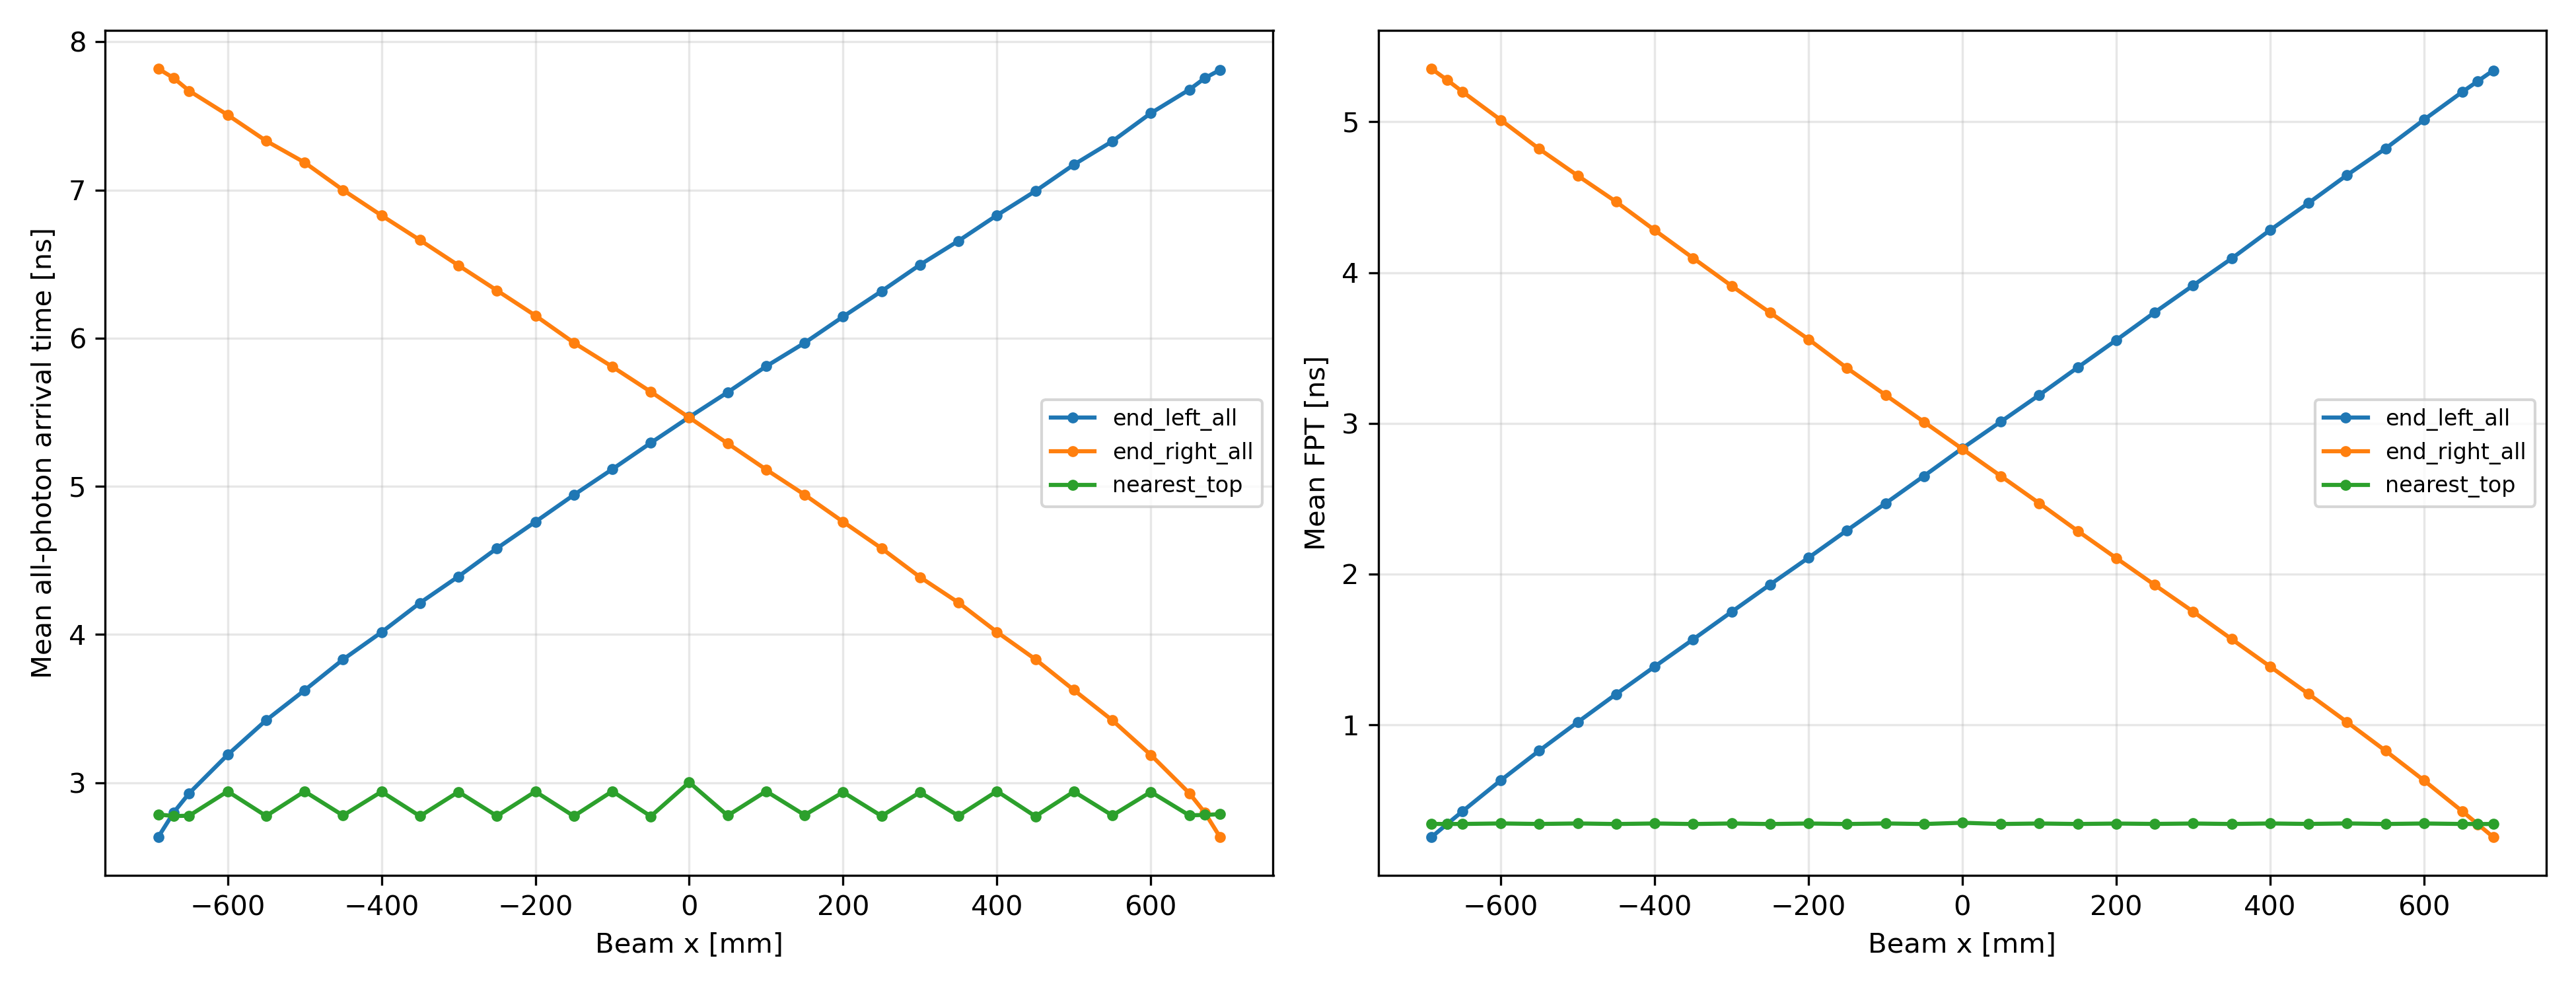
\includegraphics[width=\textwidth,height=0.68\textheight,keepaspectratio]{figs/P6_tmean_vs_x.png}\begin{block}{\footnotesize How to read this plot}
\scriptsize\textbf{Why:}~Track how the mean photon arrival time and FPT scale with beam position.
\par\textbf{Axes:}~x: beam position [mm]; y: mean arrival time [ns] and mean FPT [ns].
\par\textbf{Takeaway:}~Both estimators increase with track-to-End distance; the mean is more tail-biased than FPT and yields a larger apparent slope.
\end{block}

\end{frame}
\section{Window effect and timing}
\begin{frame}{Nearest-Top Landau/Moyal MPVs at key positions}

\centering\small
\begin{tabular}{rrrrr}\toprule
$x$ [mm] & channel & MPV [Npe] & Landau width [Npe] & $\chi^2/ndf$ \\ \midrule
-690 & 16 & $304.4\pm1.0$ & $26.9\pm0.9$ & 1.76 \\
-650 & 18 & $302.4\pm1.0$ & $26.3\pm0.9$ & 1.04 \\
-400 & 31 & $356.9\pm1.1$ & $29.3\pm1.0$ & 1.33 \\
+0 & 51 & $355.4\pm1.1$ & $26.7\pm0.9$ & 2.07 \\
+400 & 70 & $356.4\pm1.2$ & $29.1\pm1.0$ & 1.51 \\
+650 & 83 & $304.1\pm1.0$ & $26.6\pm0.9$ & 1.61 \\
+690 & 85 & $304.7\pm1.0$ & $25.6\pm0.9$ & 1.31 \\
\bottomrule\end{tabular}
\begin{block}{Interpretation}
The right tail originates primarily from Landau-like energy-loss fluctuations; Poisson
counting dominates only in the few-PE limit. MPVs are future inputs for the pending
test-beam ToT(NPE) calibration comparison.
\end{block}

\end{frame}
\begin{frame}{Window-track collection effect: mechanism}

\begin{columns}[T]
\column{0.52\textwidth}
\begin{itemize}\small
  \item Top SiPMs couple through index-matched windows
        ($6\times6$ mm$^2$) in the +Y Mylar face.
  \item First-pass photon collection depends on the solid angle
        subtended by the window from the muon track (geometric
        working hypothesis, consistent with five-run pattern).
  \item Empirically: a track at $\pm2$ mm from the window centre
        collects $\approx9.8$\% more $N_{pe}$ ($\approx12\,\sigma$);
        null at centre and at the midpoint; symmetric in mirror (C2).
  \item Scan positions with $x\equiv10\pmod{20}$ mm fall at
        $\pm2$ mm from a window centre --- hence the
        ``(window-track exception)'' label in the tables.
  \item Effect is local, symmetric, characterised and bounded:
        localization diagonal and channel map remain valid.
\end{itemize}
\column{0.46\textwidth}
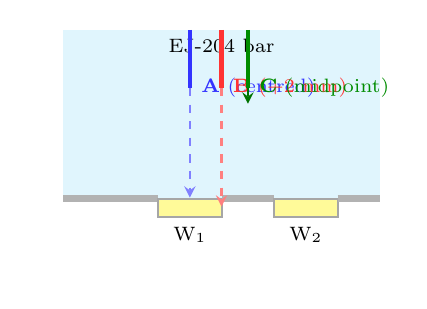
\begin{tikzpicture}[scale=0.67,>=stealth,font=\scriptsize]
  \fill[cyan!12] (-3,0) rectangle (3,3.2);
  \node at (0,2.9) {EJ-204 bar};
  \draw[line width=2.5pt,gray!60] (-3,0) -- (-1.2,0);
  \fill[yellow!40,draw=gray!70,line width=0.7pt] (-1.2,-0.35) rectangle (0,0);
  \draw[line width=2.5pt,gray!60] (0,0) -- (1.0,0);
  \fill[yellow!40,draw=gray!70,line width=0.7pt] (1.0,-0.35) rectangle (2.2,0);
  \draw[line width=2.5pt,gray!60] (2.2,0) -- (3,0);
  \node[below] at (-0.6,-0.35) {W$_1$};
  \node[below] at (1.6,-0.35) {W$_2$};
  % Track A: centred
  \draw[ultra thick,blue!80] (-0.6,3.2) -- (-0.6,2.1)
        node[right,blue!80] {\textbf{A} (centred)};
  \draw[->,thick,blue!50,dashed] (-0.6,2.1) -- (-0.6,0.02);
  % Track B: +2 mm
  \draw[ultra thick,red!80] (0.0,3.2) -- (0.0,2.1)
        node[right,red!80] {\textbf{B} ($+2$ mm)};
  \draw[->,thick,red!50,dashed] (0.0,2.1) -- (0.0,-0.15);
  % Track C: midpoint
  \draw[ultra thick,green!55!black] (0.5,3.2) -- (0.5,2.1)
        node[right,green!55!black] {\textbf{C} (midpoint)};
  \draw[->,thick,green!45!black,dashed] (0.5,2.1) -- (0.5,1.8);
  \node[below,align=center] at (-3.5,-1.2) {};
\end{tikzpicture}
\end{columns}
\begin{alertblock}{Consequence for the scan}
Track B subtends a larger first-pass solid angle to W$_1$; fewer multiple
reflections $\Rightarrow$ higher $N_{pe}$ at the nearest channel.
At midpoint (C) both windows contribute equally and the effect is null.
\end{alertblock}

\end{frame}
\begin{frame}{Window-track collection effect: five-run test}

\begin{columns}[T]\column{0.47\textwidth}
\scriptsize\resizebox{\textwidth}{!}{\begin{tabular}{lrr}\toprule
Run & contrast [Npe] & significance \\ \midrule
Existing -650 & $34.60\pm2.94$ & $11.78$ \\
A -652 center & $2.86\pm2.65$ & $1.08$ \\
B -642 midpoint & $-0.33\pm3.35$ & $-0.10$ \\
C1 -648 (+4 mm) & $21.08\pm3.20$ & $6.59$ \\
C2 -654 mirror & $34.38\pm2.95$ & $11.64$ \\
\bottomrule\end{tabular}}
\column{0.51\textwidth}
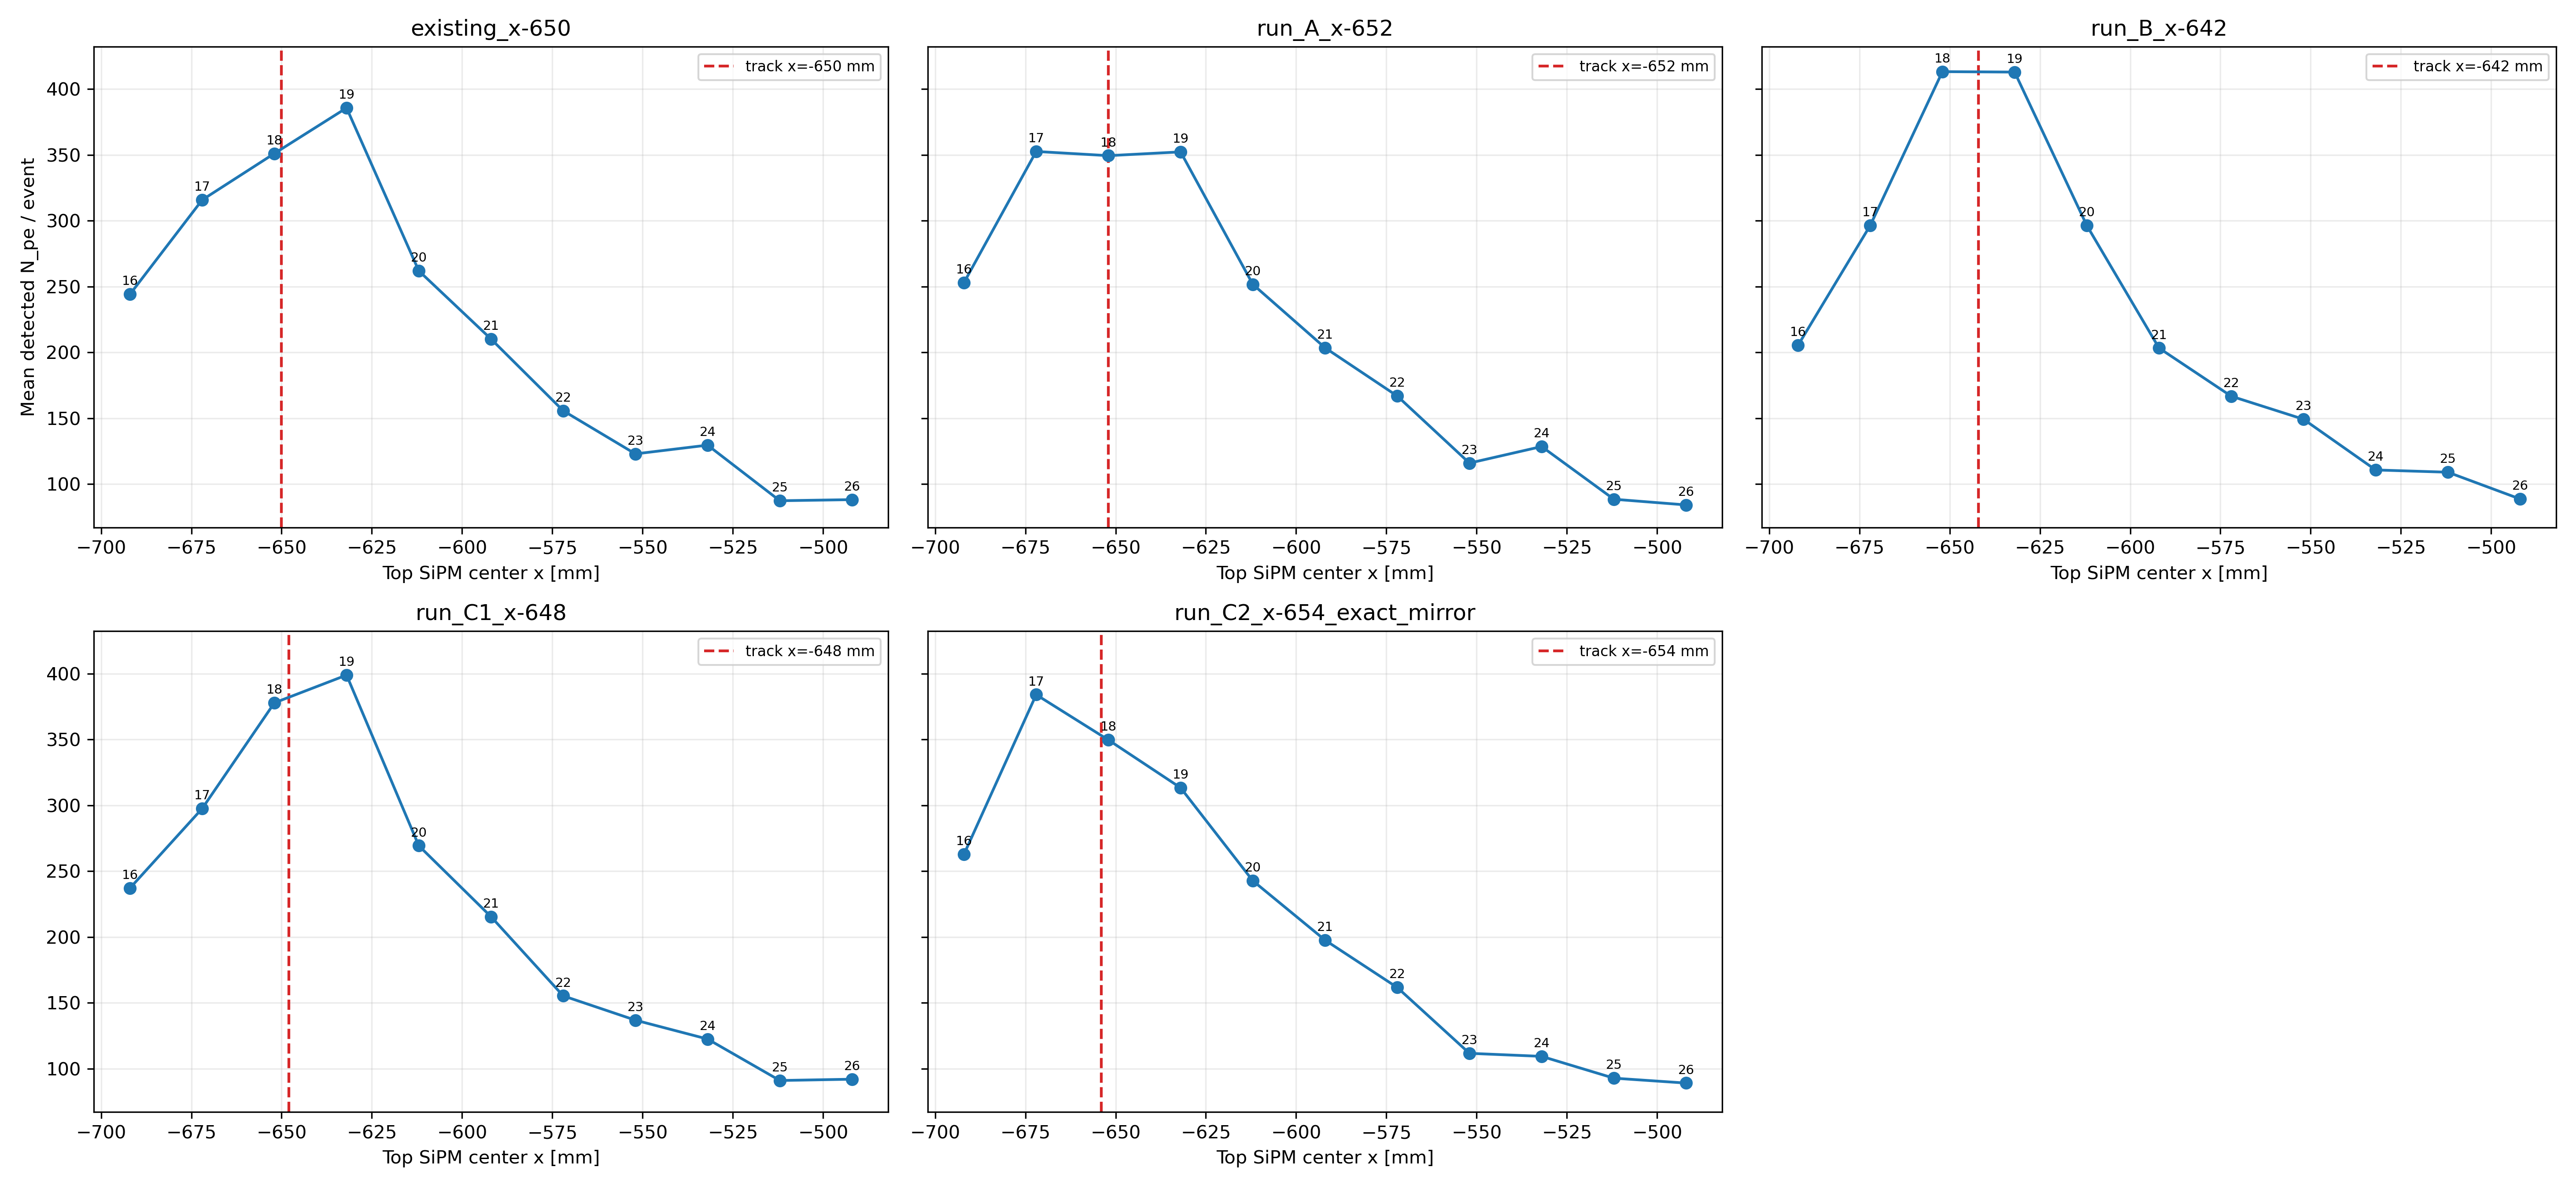
\includegraphics[width=\textwidth]{figs/exec08b_window_dip_profiles.png}
\end{columns}
\begin{block}{Finding}
Local symmetric $\pm2$ mm effect: about 9.8\% at about 12 sigma; null when centered
and at midpoint. The scan and channel map remain valid.
\end{block}

\end{frame}
\begin{frame}{Intrinsic End SUM4 timing}
\centering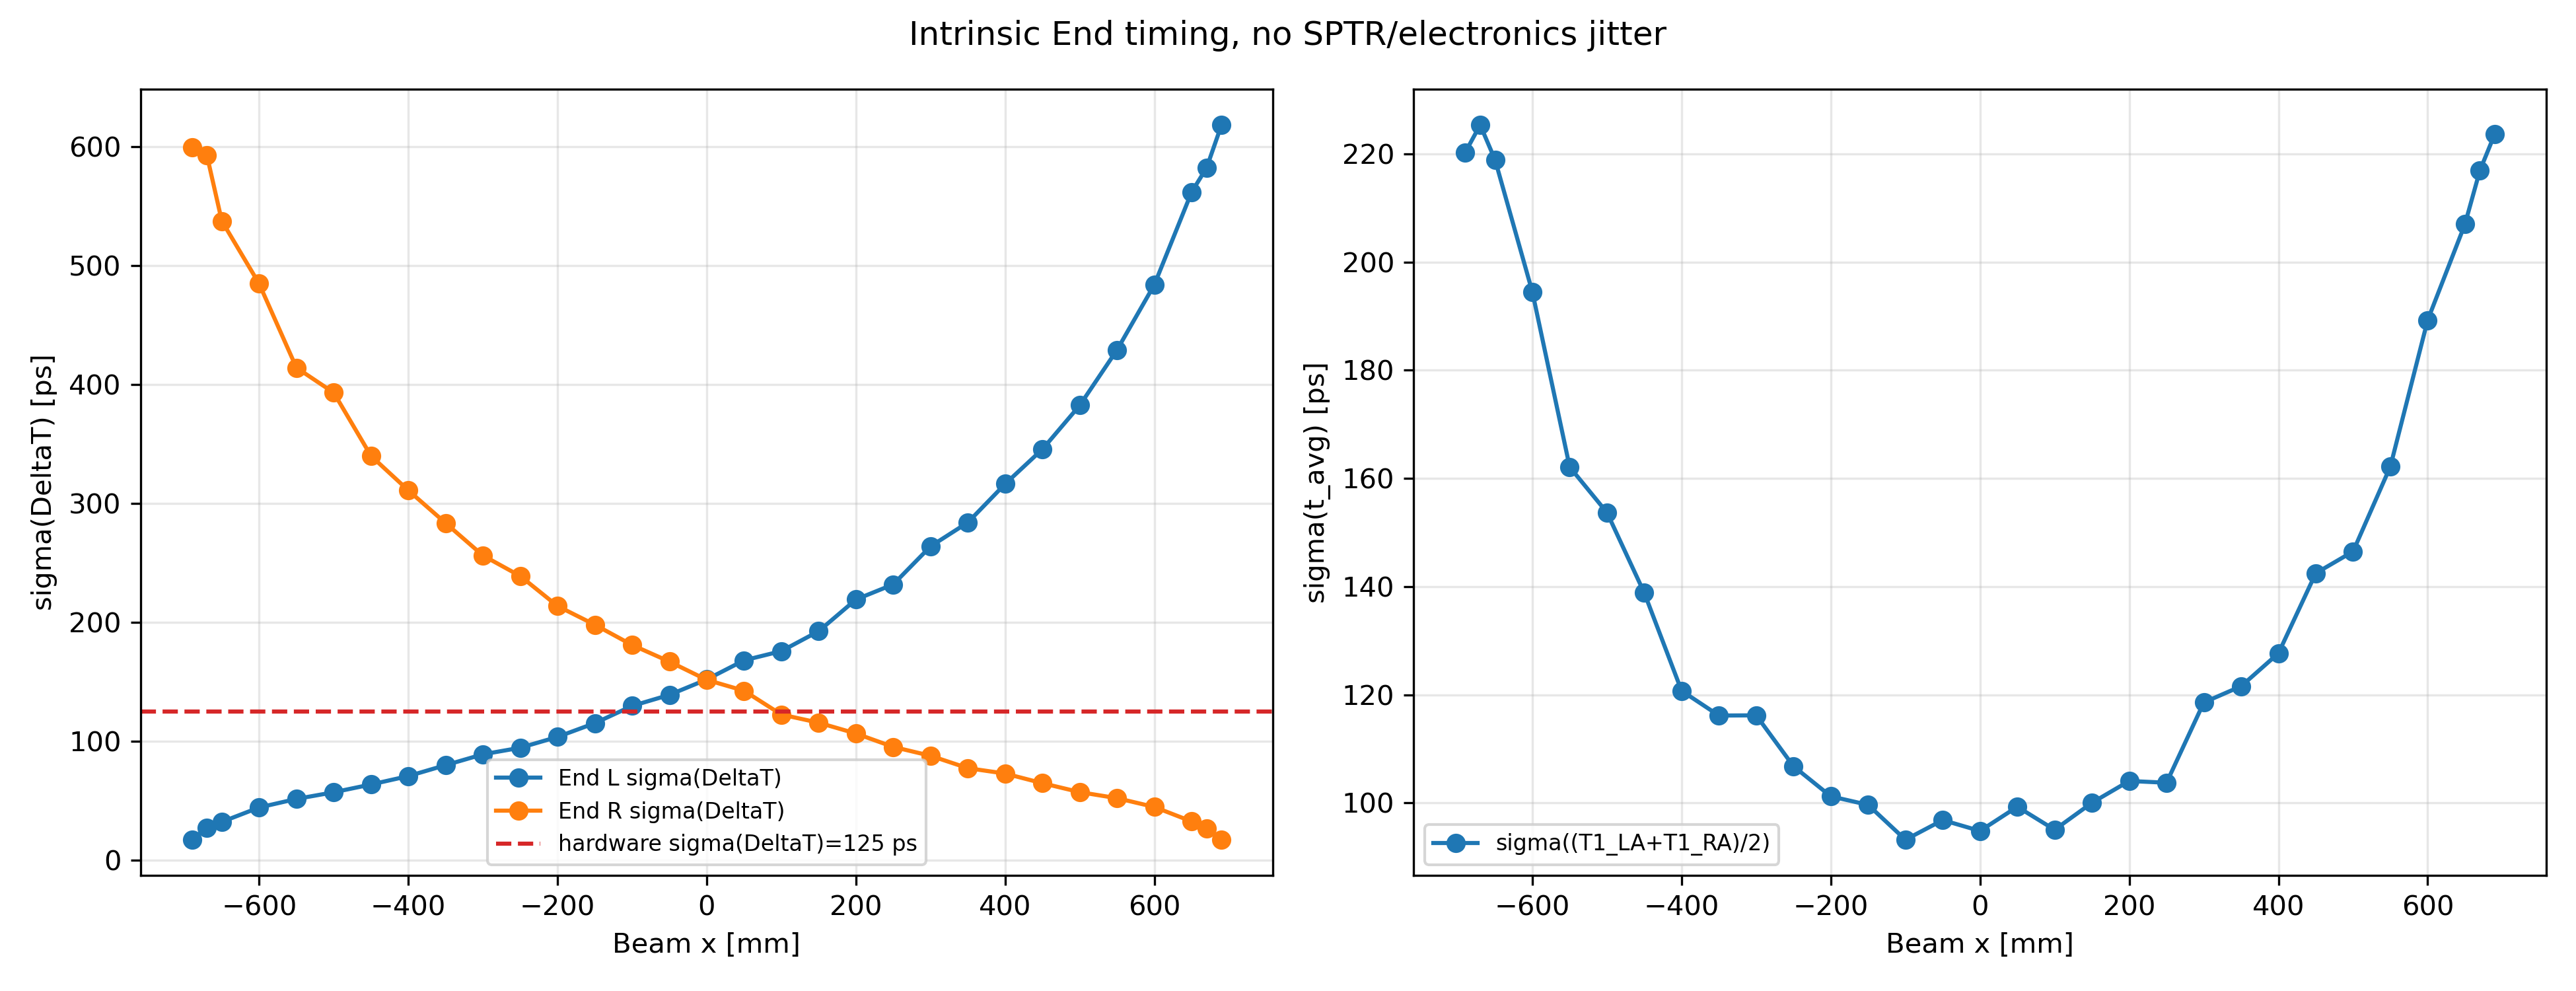
\includegraphics[width=\textwidth,height=0.60\textheight,keepaspectratio]{figs/P7_deltaT_end.png}\par\scriptsize $\sigma_{group}=\sigma(\Delta T_{AB})/\sqrt{2}$; no SPTR/jitter. The 88 ps hardware context is not directly comparable.
\begin{block}{\footnotesize How to read this plot}
\scriptsize\textbf{Why:}~Measure the intrinsic Same-End SUM4 coincidence timing resolution without SPTR or electronics jitter.
\par\textbf{Axes:}~x: beam position [mm]; y: $\sigma_{group}$ [ps]. Lines for left and right End groups.
\par\textbf{Takeaway:}~$\sigma_{group}$ decreases toward the nearer End (higher $N_{pe}$, earlier FPT); consistent with photon-counting scaling $\propto1/\sqrt{N_{pe}}$.
\end{block}

\end{frame}
\begin{frame}{End arrival-time tails without any time acceptance window: narrower EndTop is physical}

\begin{columns}[T]\column{0.48\textwidth}
\scriptsize\resizebox{\textwidth}{!}{\begin{tabular}{rrrrr}\toprule
$x$ & side & EndTop [ps] & End-only [ps] & ratio \\ \midrule
-400 & L & $50.0\pm0.8$ & $66.1\pm0.5$ & $0.756\pm0.013$ \\
-400 & R & $219.9\pm3.5$ & $248.4\pm1.8$ & $0.885\pm0.015$ \\
+0 & L & $107.5\pm1.7$ & $131.4\pm0.9$ & $0.818\pm0.014$ \\
+0 & R & $107.2\pm1.7$ & $129.5\pm0.9$ & $0.828\pm0.014$ \\
+400 & L & $223.8\pm3.5$ & $247.5\pm1.8$ & $0.904\pm0.016$ \\
+400 & R & $51.5\pm0.8$ & $65.9\pm0.5$ & $0.781\pm0.014$ \\
\bottomrule\end{tabular}}
\column{0.50\textwidth}
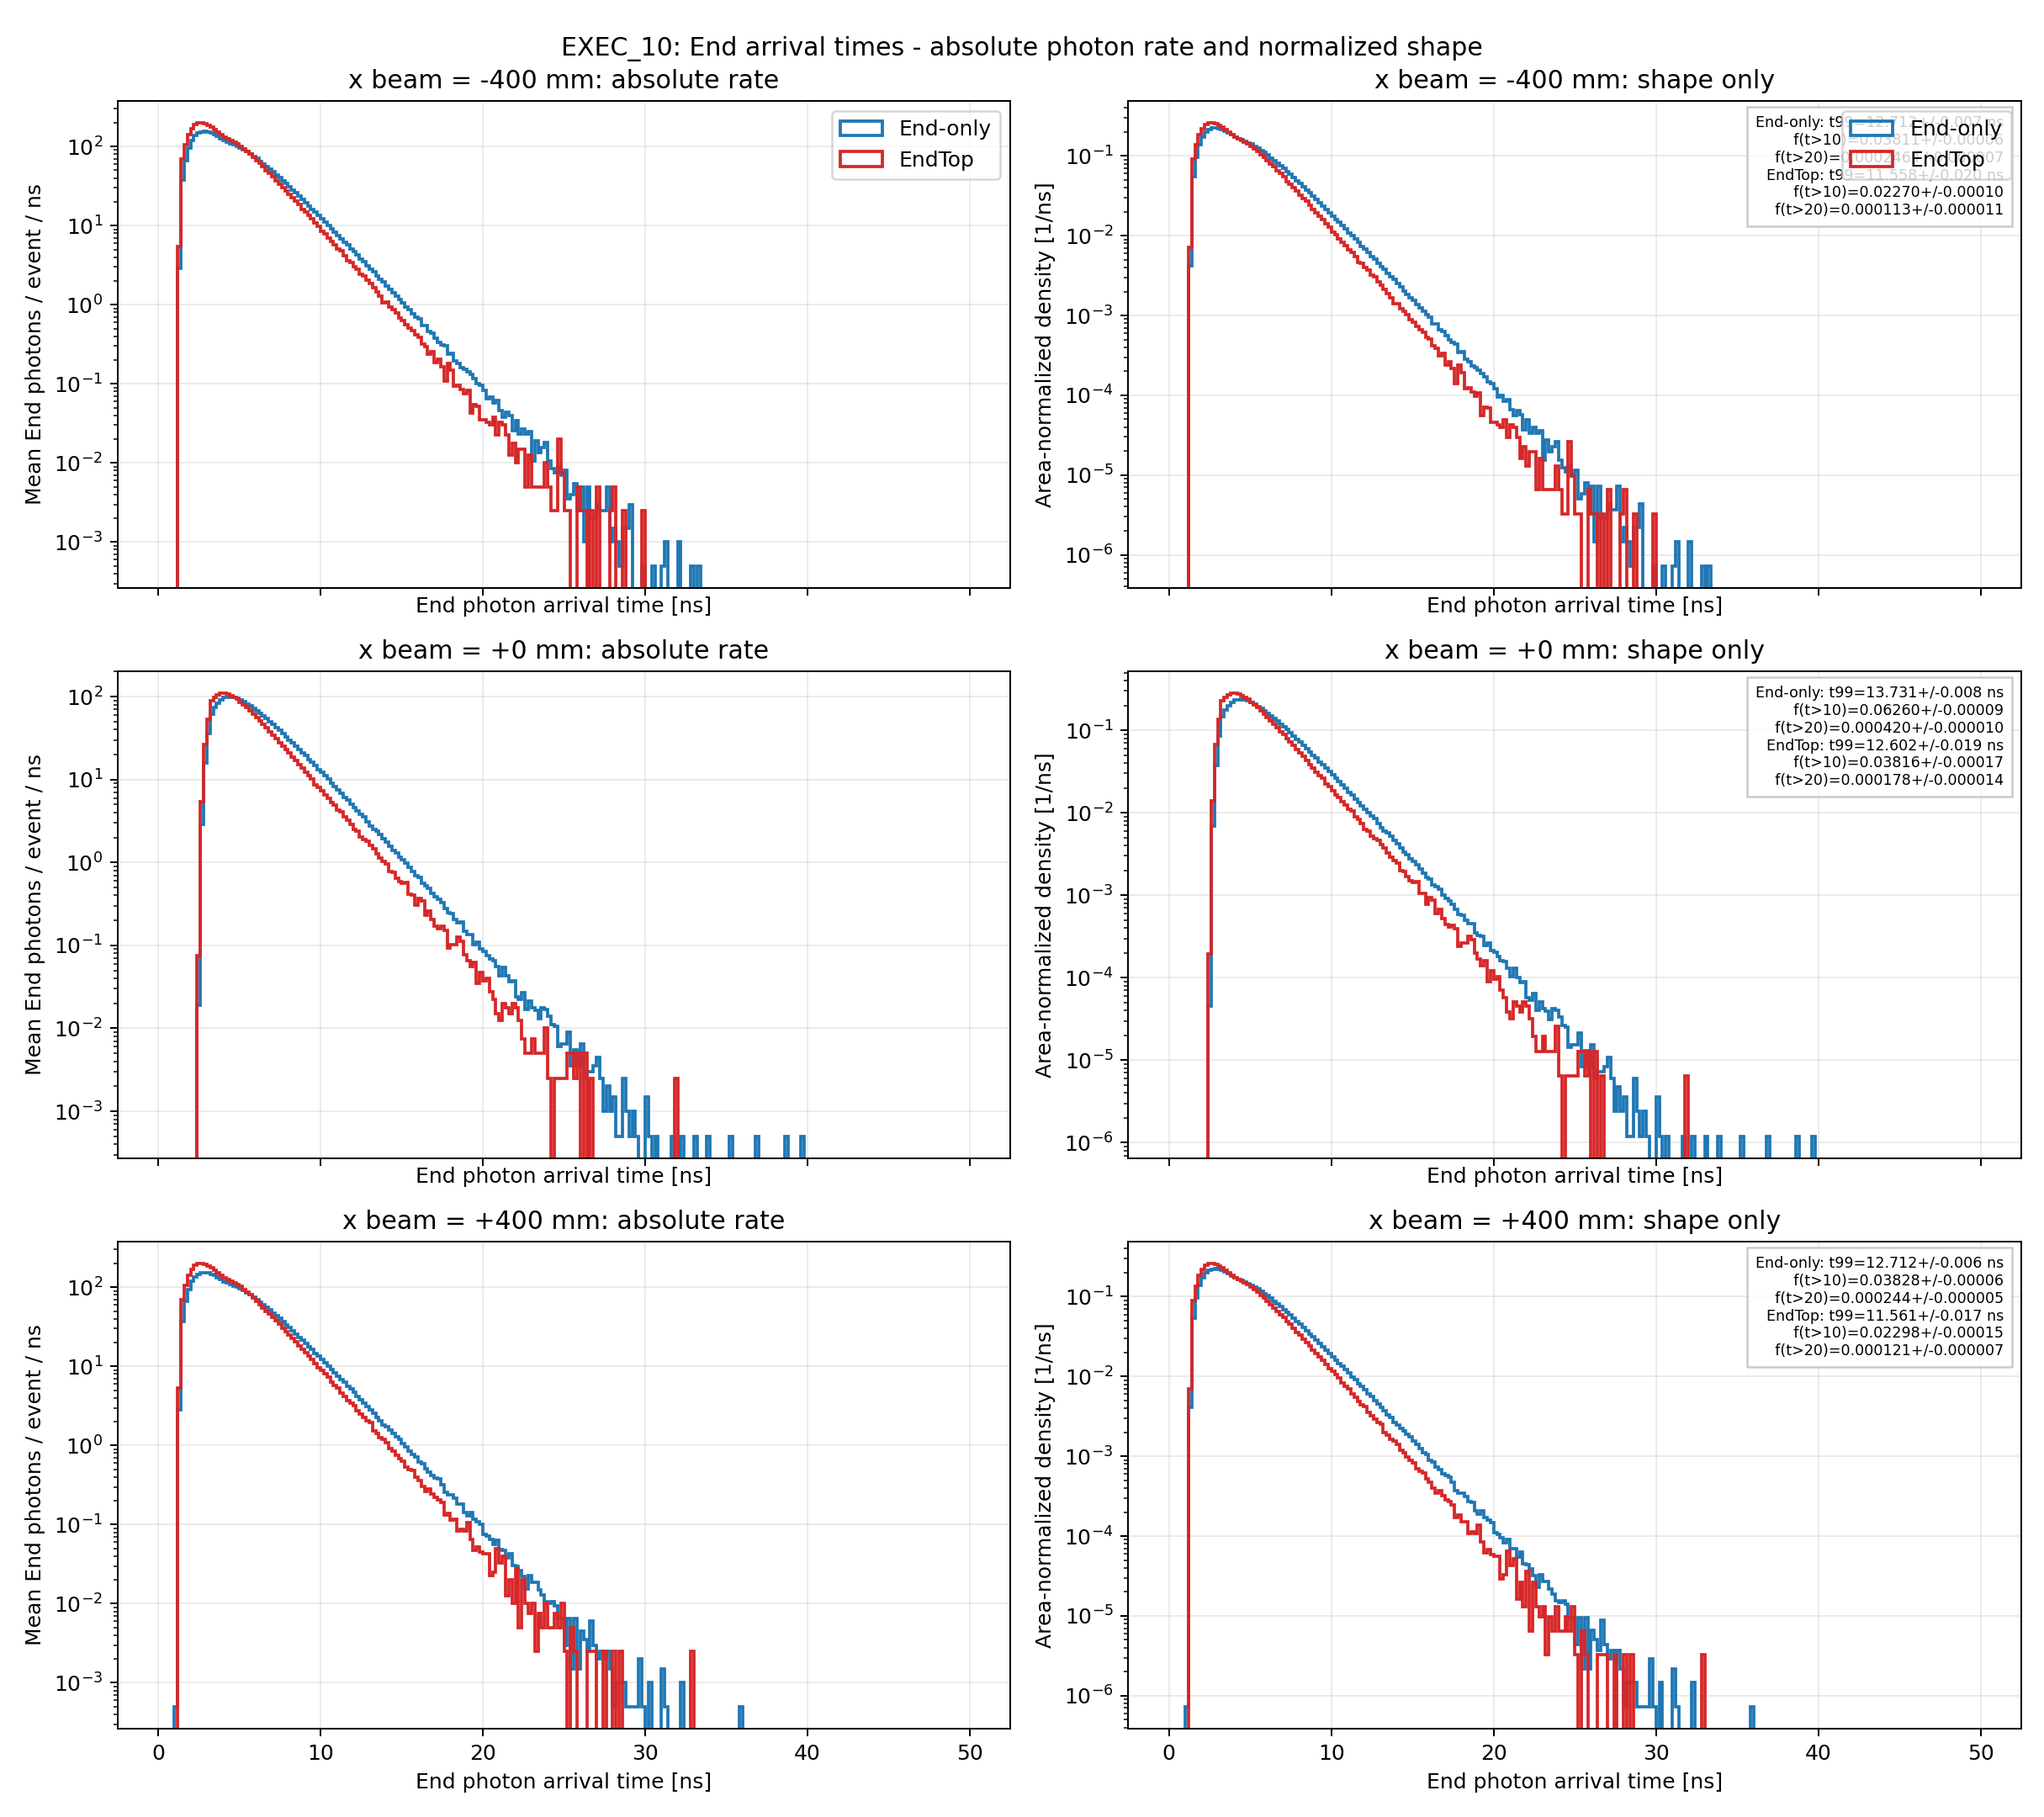
\includegraphics[width=0.88\textwidth]{figs/exec09_tail_comparison.png}
\end{columns}
\begin{alertblock}{Confirmed mechanism}
Across $x=0,\pm400$ mm, EndTop lowers $t99$ by
1.14 ns and suppresses late fractions
at more than 10.3 sigma.
\end{alertblock}
\begin{block}{\footnotesize No time acceptance window}
\scriptsize
In all published analyses (EXEC\_08b--EXEC\_09), End-photon arrival times
are reported without any $t<t_{max}$ acceptance cut: all detected End photons
in the ROOT TTree are used
(\texttt{exec08b\_timing\_gate.py}, \texttt{exec09\_timing\_mechanism.py}).
The EndTop tail narrowing persists over the full arrival-time range
and is therefore physical, not an analysis artefact.
\end{block}

\end{frame}
\begin{frame}{Apparent timing slopes: no propagation estimator passes}

\begin{columns}[T]\column{0.62\textwidth}
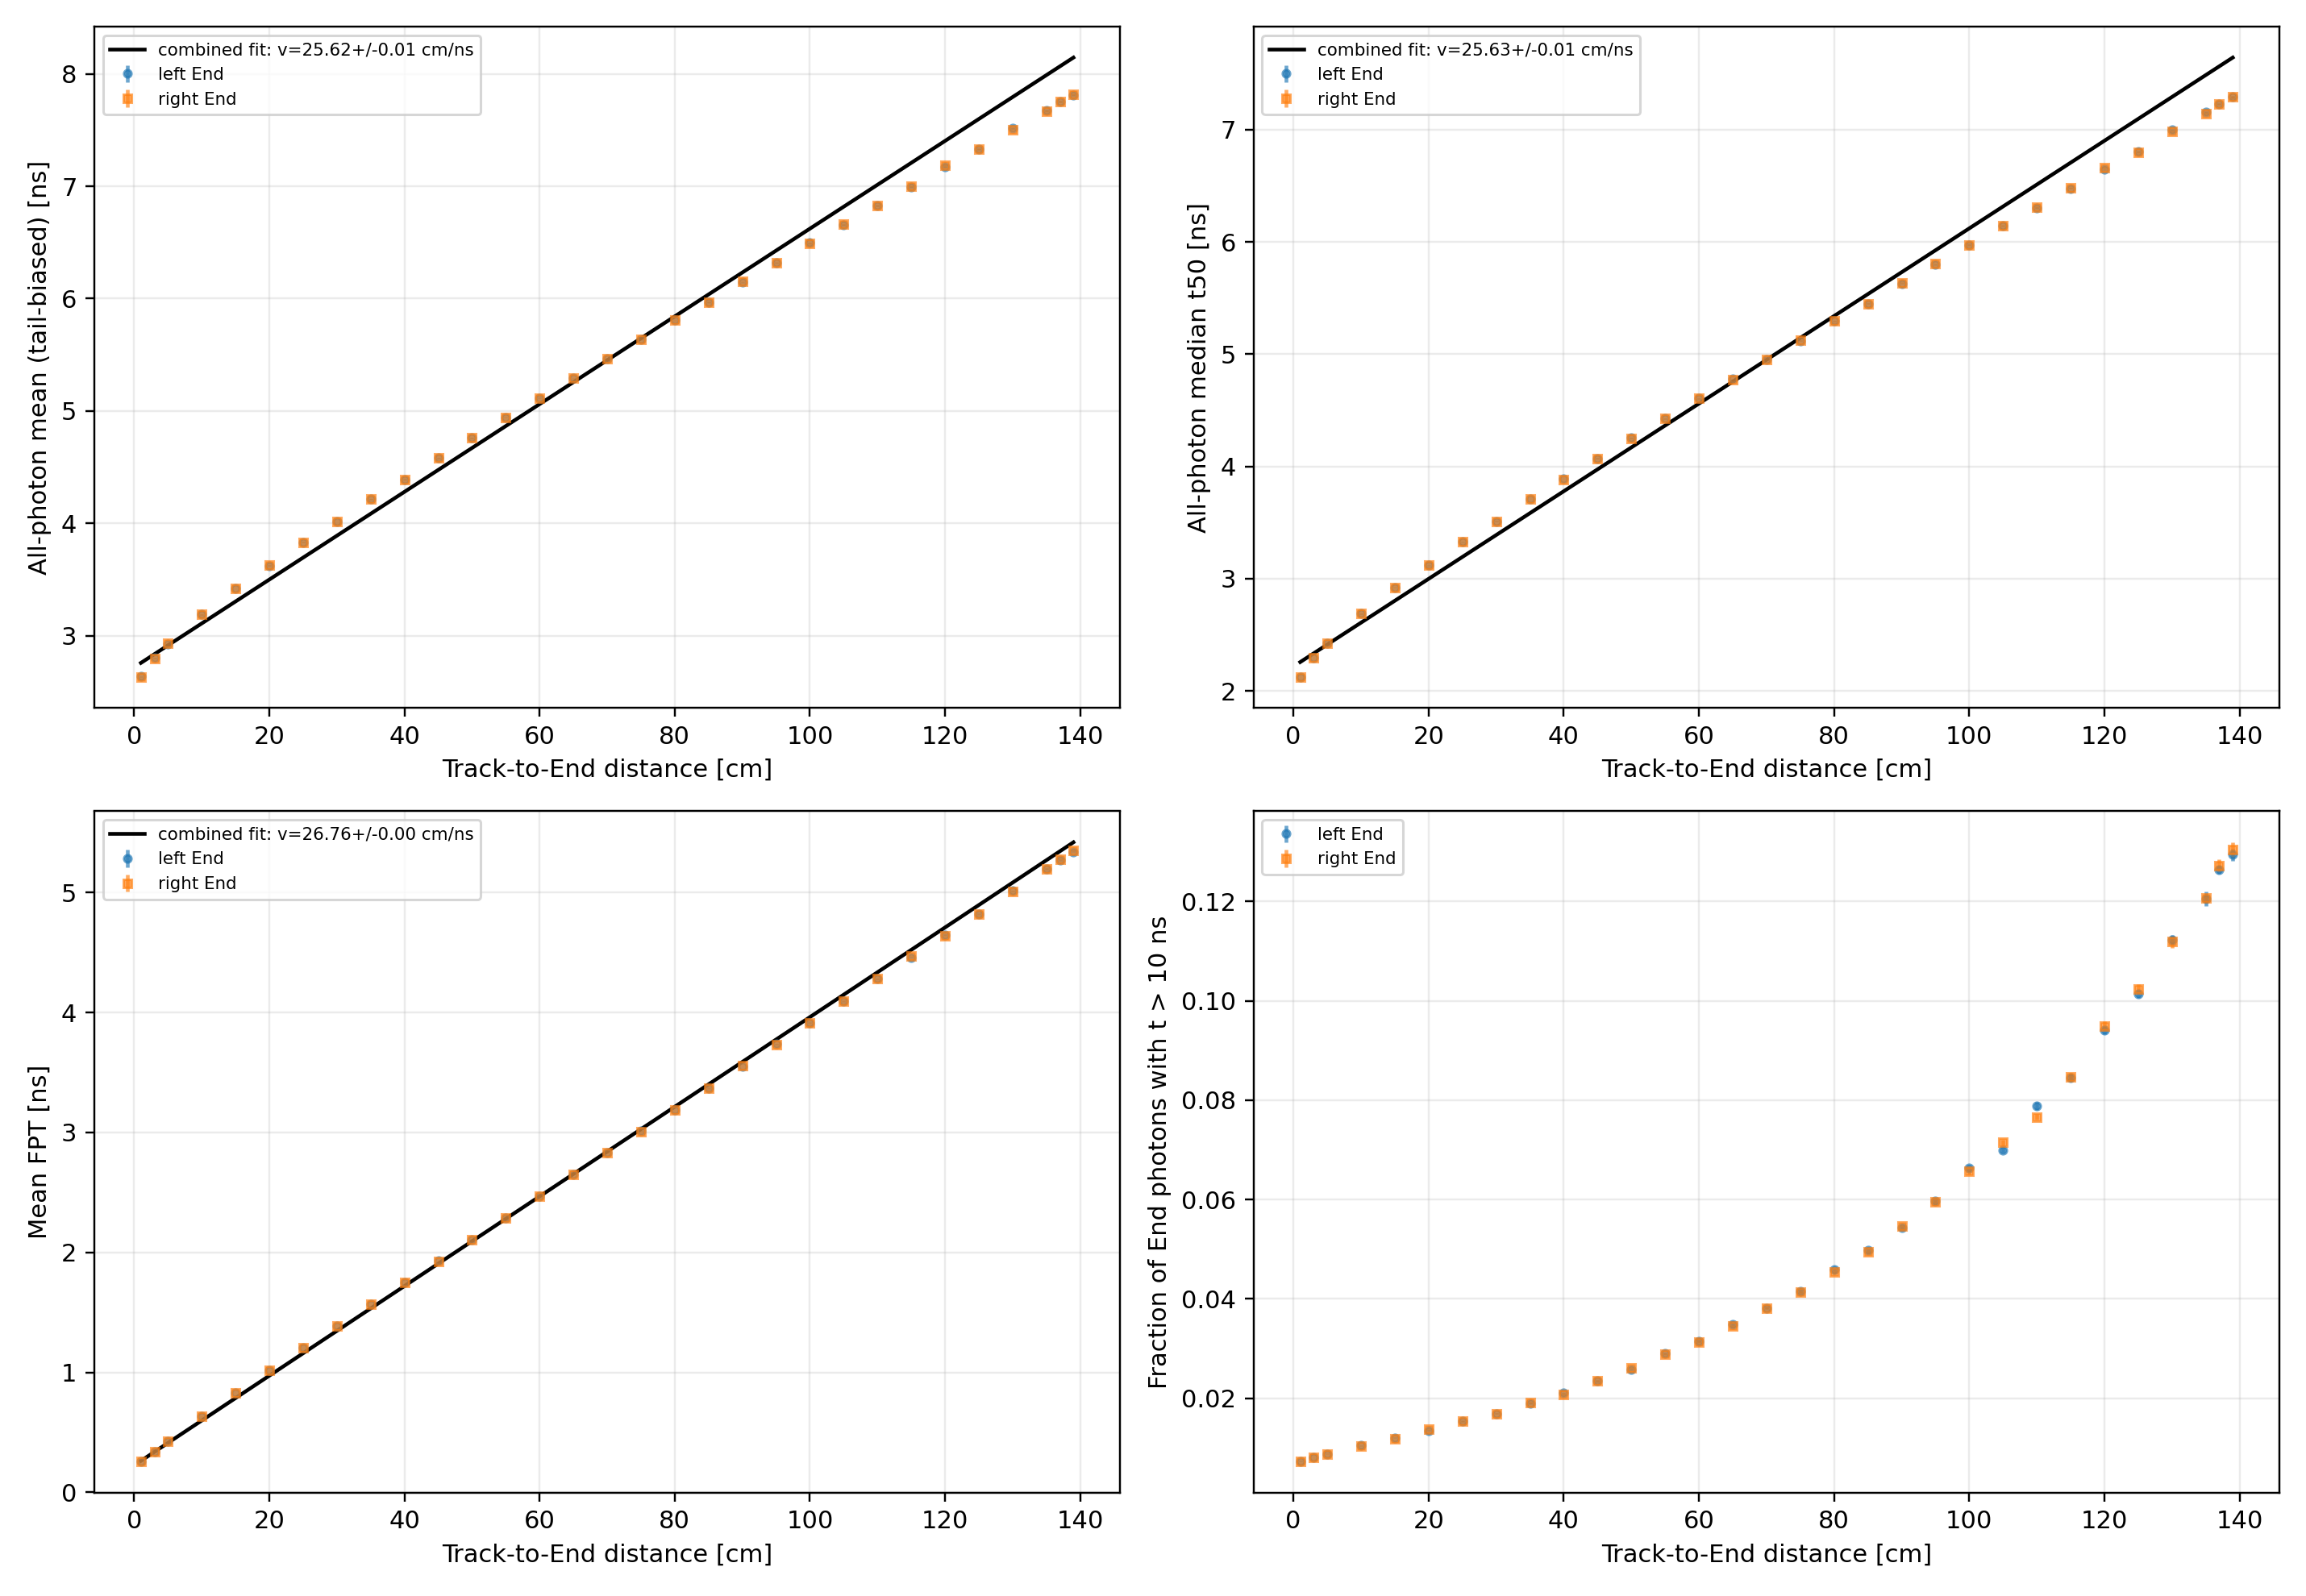
\includegraphics[width=\textwidth]{figs/exec10_velocity_estimators.png}
\column{0.36\textwidth}
\scriptsize\resizebox{\textwidth}{!}{\begin{tabular}{lrr}\toprule
Estimator & slope-derived [cm/ns] & $\chi^2/ndf$ \\ \midrule
all-photon mean & $25.616\pm0.005$ & 3189.9 \\
all-photon $t_{50}$ & $25.625\pm0.005$ & 3615.1 \\
mean FPT & $26.758\pm0.003$ & 1002.6 \\
\bottomrule\end{tabular}}
\begin{alertblock}{Refuted predictions}
Mean FPT is not close to $c/n\simeq19$ cm/ns. The fixed-threshold $f(t>10\,ns)$
increases with distance. Every global line fit is rejected.
\end{alertblock}
\begin{block}{\footnotesize How to read this plot}
\scriptsize\textbf{Why:}~Test whether any timing estimator reveals a light-propagation velocity.
\par\textbf{Axes:}~x: track-to-End distance [cm]; y: timing estimator [ns]. Fits shown.
\par\textbf{Takeaway:}~No estimator yields a statistically acceptable propagation-velocity fit; the slope is dominated by the long late-tail bias.
\end{block}

\end{columns}

\end{frame}
\begin{frame}{Top readout: analytic timing estimate only}

\centering\small
\begin{tabular}{rrr}\toprule
$x$ [mm] & nearest Top $N_{pe}$ & $\sigma_{t,est}$ [ps] \\ \midrule
-690 & $350.9\pm2.0$ & $59.92\pm0.17$ \\
-650 & $351.0\pm2.0$ & $59.91\pm0.17$ \\
-400 & $411.3\pm2.3$ & $55.35\pm0.16$ \\
+0 & $407.3\pm2.2$ & $55.62\pm0.15$ \\
+400 & $411.4\pm2.4$ & $55.34\pm0.16$ \\
+650 & $350.9\pm2.1$ & $59.93\pm0.18$ \\
+690 & $353.0\pm2.0$ & $59.75\pm0.17$ \\
\bottomrule\end{tabular}
\vspace{0.35cm}
\begin{block}{Definition, derivation, and scope}
$\sigma_{t,est}=\sqrt{\tau_r\cdot\tau_d}/\sqrt{N_{pe}}
=1.122\,\mathrm{ns}/\sqrt{N_{pe}}$
\par\scriptsize
Standard single-photodetector timing scaling for a threshold at low $N_{pe}$ with
double-exponential emission ($\tau_r\cdot\tau_d$ product, rise $\times$ decay;
see e.g.\ Knoll, \emph{Radiation Detection and Measurement}, ch.\ 8).
$\tau_r=0.7$ ns, $\tau_d=1.8$ ns from the verified SSLG4 MPT.
This is an \textbf{analytic orientation only}, not a simulated timing resolution.
Top has no test-beam counterpart.
\end{block}
\vspace{0.25cm}
\begin{block}{\footnotesize Analytic estimate vs.\ simulated $\sigma(t_4)$ (T4)}
\scriptsize\begin{tabular}{rcc}\toprule
$x$ [mm] & $\sigma_{t,est}$ [ps] (analytic) & $\sigma(t_4)$ [ps] (simulated)\\ \midrule
-690 & $60\pm0$ & — \\
-650 & $60\pm0$ & — \\
-400 & $55\pm0$ & — \\
+0 & $56\pm0$ & — \\
+400 & $55\pm0$ & — \\
+650 & $60\pm0$ & — \\
+690 & $60\pm0$ & — \\
\bottomrule\end{tabular}
\par\scriptsize $\sigma(t_4)$ is the photon-counting lower bound; $\sigma_{t,est}$
includes the SPE pulse-shape contribution ($\sqrt{\tau_r\tau_d}$) and is
therefore larger --- consistent with the SPE-convolution jitter seen in $\sigma_{group}$.
\end{block}

\end{frame}
\begin{frame}{Numerical conclusions}

\small\begin{itemize}
 \item At center: End sum $389.6\pm2.1$, nearest Top $407.3\pm2.2$;
       at $x=-690$ mm: End sum $3404.2\pm18.3$, nearest Top $350.9\pm2.0$.
 \item $\lambda_{eff}$: L $33.14\pm0.03$ cm,
       R $33.06\pm0.03$ cm
       ($\ll$ ABSLENGTH $=160$ cm; system effective length, not material property).
 \item Nearest-Top $F=1+(0.062162\pm0.000107)\langle N_{pe}\rangle$
       ($\chi^2/ndf=1.76$): Landau energy-loss fluctuations dominate.
       Same mechanism: asymmetric $N_{pe}$ spectrum (Moyal$\otimes$Gauss) and $F>1$.
 \item Intrinsic End $\sigma_{group}$: mean 148.3 ps,
       range 12.1--437.3 ps.
 \item EndTop/End-only timing ratio: $0.756$
       to $0.904$; no time-acceptance window in any script.
 \item $\sigma(t_4)$ (near-End SUM4): 15--123 ps (high-$N_{pe}$ to low); pure photon-counting lower bound, factor $\sim3$ below $\sigma_{group}$ at high $N_{pe}$ due to SPE pulse-convolution jitter in the analog discriminator. Nearest-Top $\sigma(t_4)$: 8--9 ps.
 \item Four findings: window-track mechanism defined and characterised; late-tail drain confirmed;
       complete 86-channel coverage and localisation validated; $t_N$ photon-counting timing quantified.
\end{itemize}

\end{frame}
\section{Full scan, position by position}
\begin{frame}{Position x=-690 mm}

\begin{columns}[T]
  \column{0.52\textwidth}
  
\includegraphics[width=\textwidth]{figs/muon_-690mm_geometry.png}
  \column{0.46\textwidth}
  
\includegraphics[width=\textwidth]{figs/muon_-690mm_top_profile.png}
  \tiny
  \begin{tabular}{lr}
    \toprule Quantity & Value \\ \midrule
    End L $N_{pe}$ & $3363.1\pm18.1$ \\
    End R $N_{pe}$ & $41.1\pm0.3$ \\
    Nearest Top ID & 16 (window-track exception) \\
    Nearest Top $N_{pe}$ & $350.9\pm2.0$ \\
    Nearest Top $\langle t\rangle$ &
      $2.7863\pm0.0023$ ns \\
    Nearest Top FPT & $0.34278\pm0.00023$ ns \\
    \bottomrule
  \end{tabular}
\end{columns}

\end{frame}
\begin{frame}{Run 1 $|$ x = -690 mm $|$ Photon arrival $\langle N(t)\rangle$}
\centering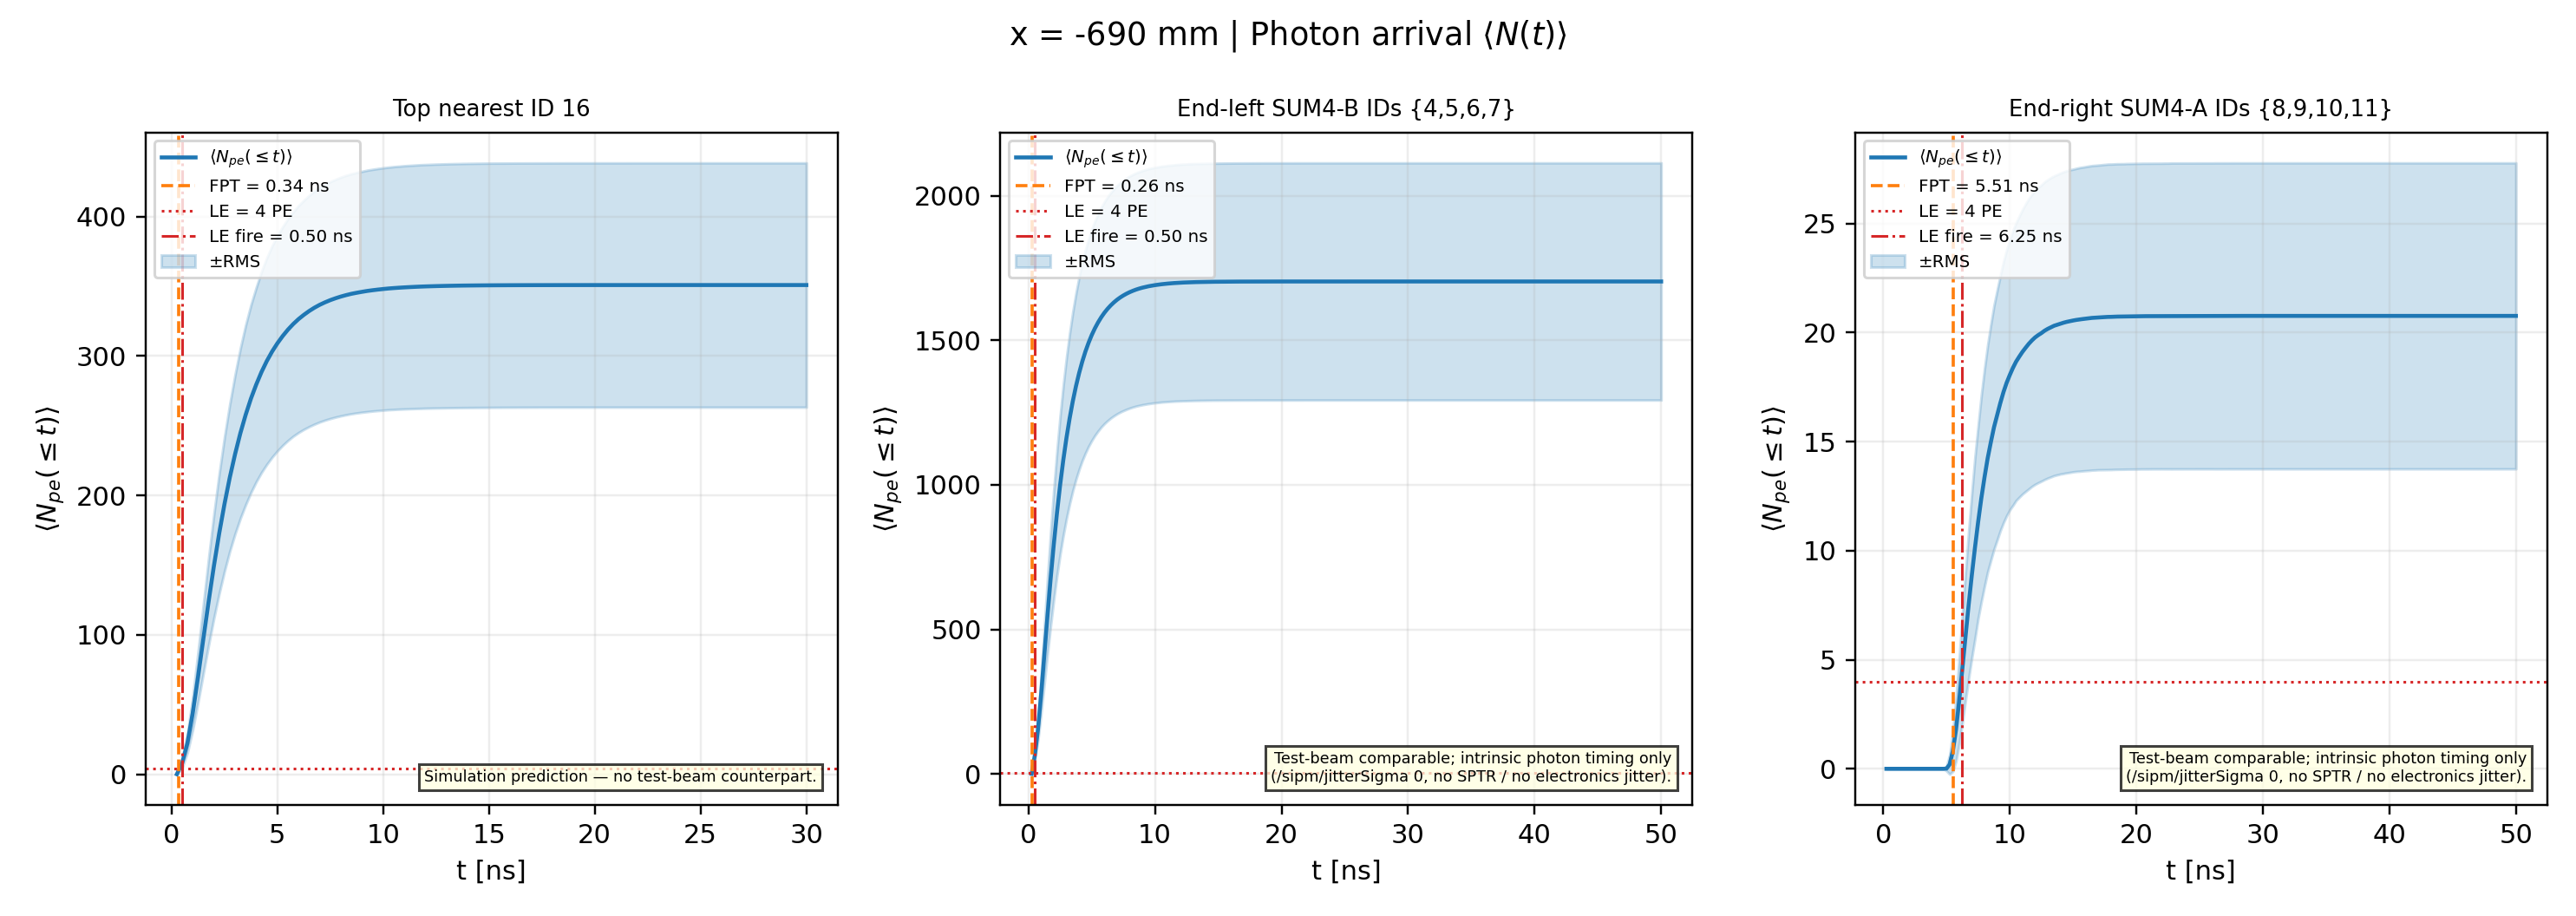
\includegraphics[width=\textwidth,height=0.78\textheight,keepaspectratio]{figs/exec11_arrival_-690mm.png}
\end{frame}
\begin{frame}{Position x=-670 mm}

\begin{columns}[T]
  \column{0.52\textwidth}
  
\includegraphics[width=\textwidth]{figs/muon_-670mm_geometry.png}
  \column{0.46\textwidth}
  
\includegraphics[width=\textwidth]{figs/muon_-670mm_top_profile.png}
  \tiny
  \begin{tabular}{lr}
    \toprule Quantity & Value \\ \midrule
    End L $N_{pe}$ & $2764.3\pm15.0$ \\
    End R $N_{pe}$ & $42.6\pm0.3$ \\
    Nearest Top ID & 17 (window-track exception) \\
    Nearest Top $N_{pe}$ & $350.4\pm2.0$ \\
    Nearest Top $\langle t\rangle$ &
      $2.7753\pm0.0023$ ns \\
    Nearest Top FPT & $0.34261\pm0.00021$ ns \\
    \bottomrule
  \end{tabular}
\end{columns}

\end{frame}
\begin{frame}{Run 2 $|$ x = -670 mm $|$ Photon arrival $\langle N(t)\rangle$}
\centering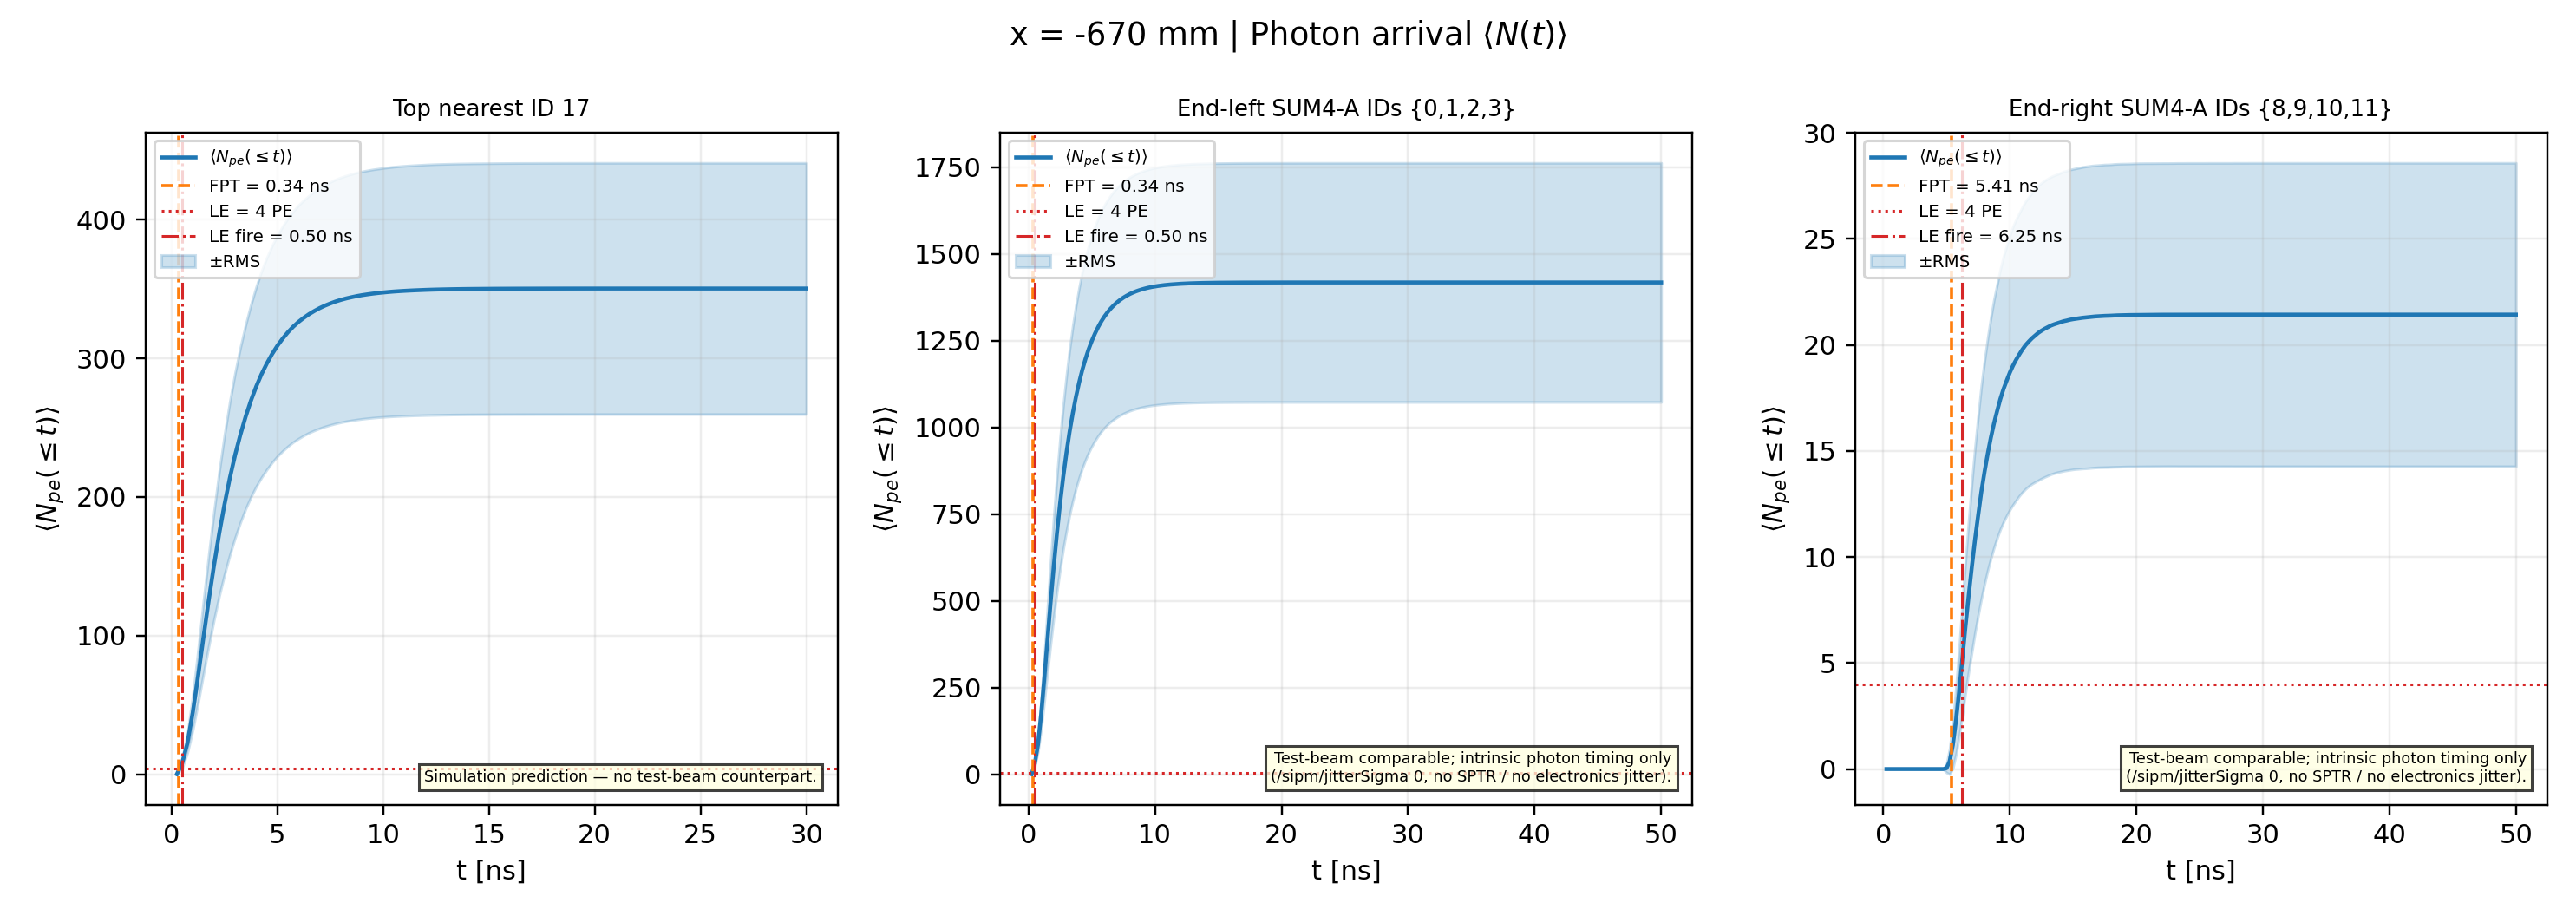
\includegraphics[width=\textwidth,height=0.78\textheight,keepaspectratio]{figs/exec11_arrival_-670mm.png}
\end{frame}
\begin{frame}{Position x=-650 mm}

\begin{columns}[T]
  \column{0.52\textwidth}
  
\includegraphics[width=\textwidth]{figs/muon_-650mm_geometry.png}
  \column{0.46\textwidth}
  
\includegraphics[width=\textwidth]{figs/muon_-650mm_top_profile.png}
  \tiny
  \begin{tabular}{lr}
    \toprule Quantity & Value \\ \midrule
    End L $N_{pe}$ & $2366.2\pm13.1$ \\
    End R $N_{pe}$ & $44.3\pm0.3$ \\
    Nearest Top ID & 18 (window-track exception) \\
    Nearest Top $N_{pe}$ & $351.0\pm2.0$ \\
    Nearest Top $\langle t\rangle$ &
      $2.7779\pm0.0023$ ns \\
    Nearest Top FPT & $0.34270\pm0.00024$ ns \\
    \bottomrule
  \end{tabular}
\end{columns}

\end{frame}
\begin{frame}{Run 3 $|$ x = -650 mm $|$ Photon arrival $\langle N(t)\rangle$}
\centering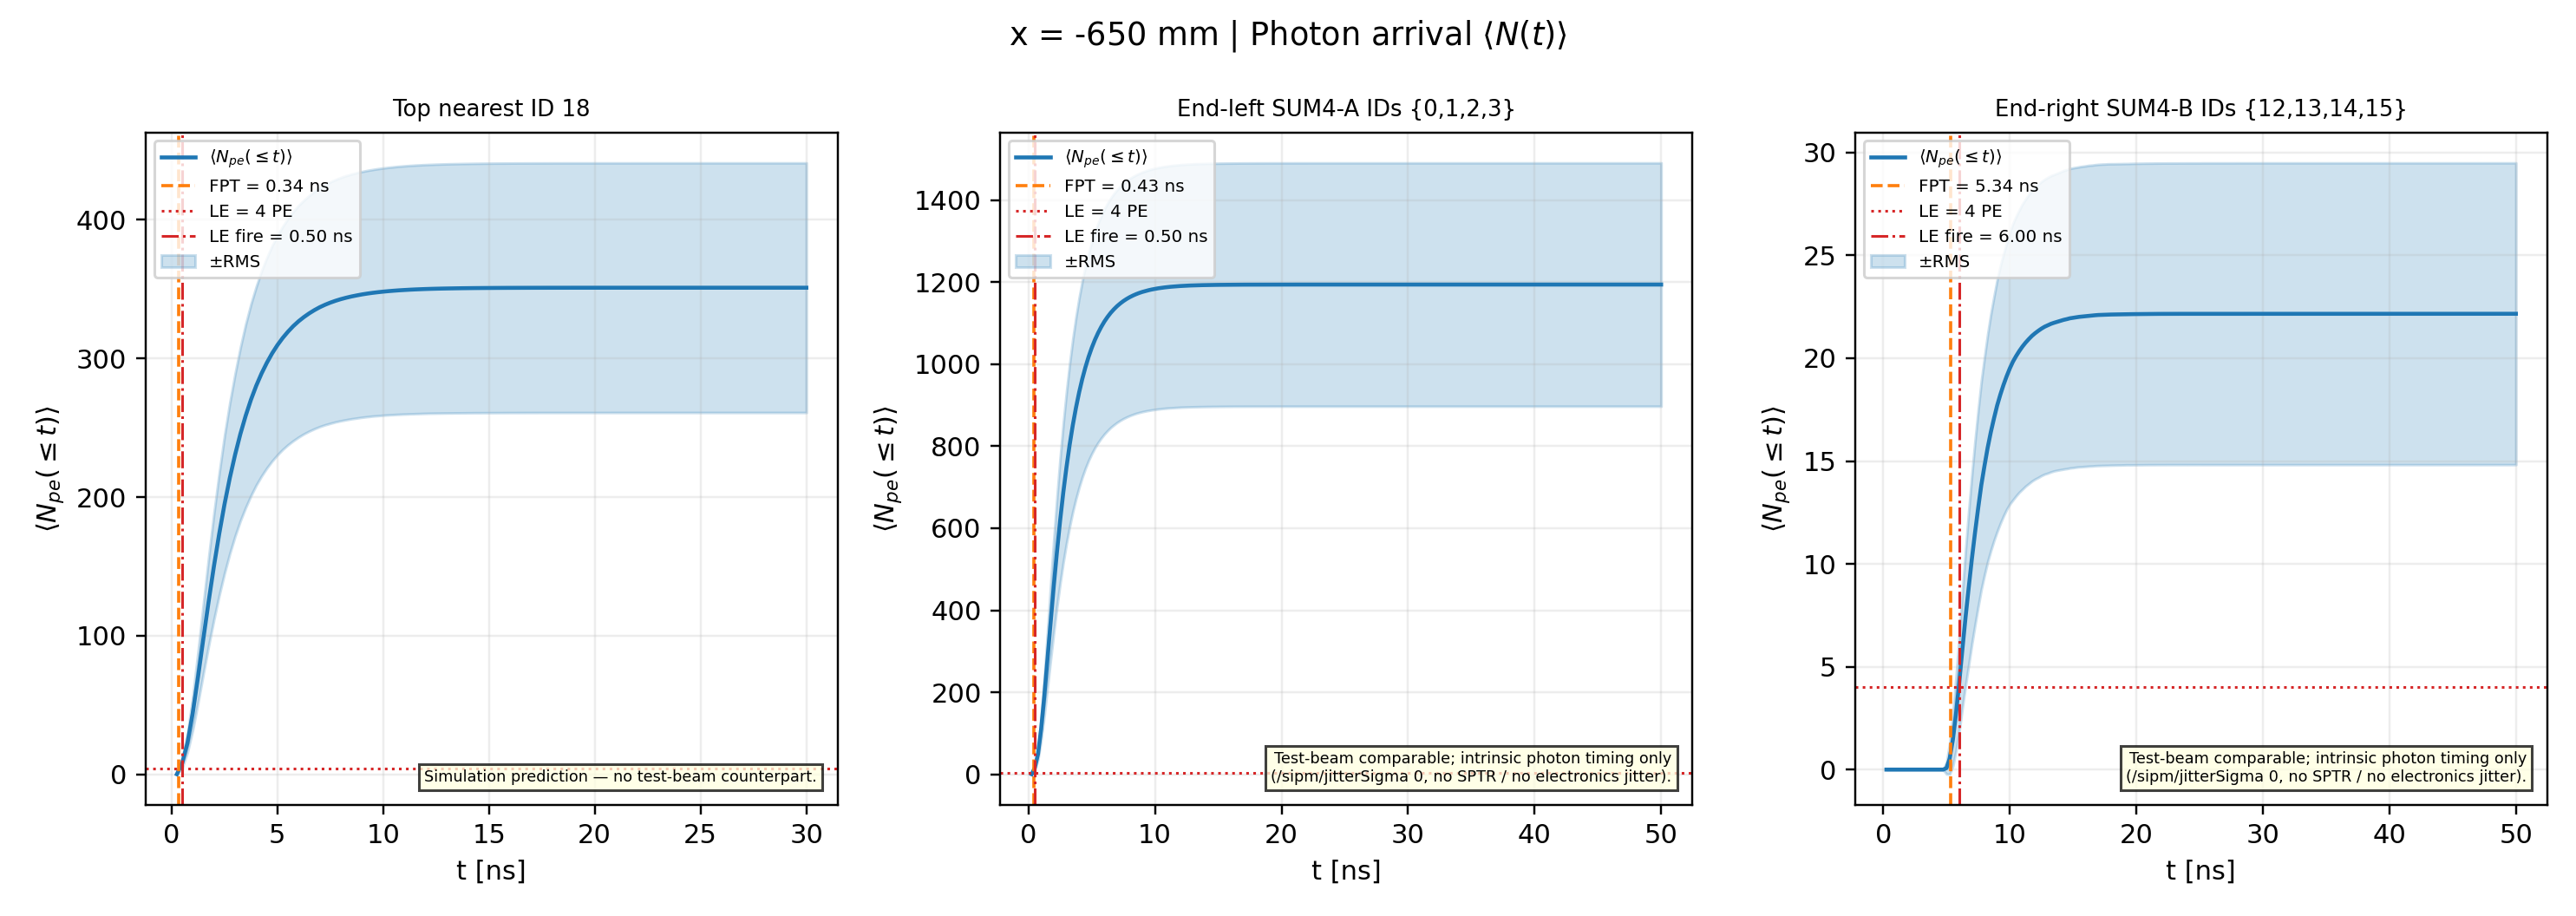
\includegraphics[width=\textwidth,height=0.78\textheight,keepaspectratio]{figs/exec11_arrival_-650mm.png}
\end{frame}
\begin{frame}{Position x=-600 mm}

\begin{columns}[T]
  \column{0.52\textwidth}
  
\includegraphics[width=\textwidth]{figs/muon_-600mm_geometry.png}
  \column{0.46\textwidth}
  
\includegraphics[width=\textwidth]{figs/muon_-600mm_top_profile.png}
  \tiny
  \begin{tabular}{lr}
    \toprule Quantity & Value \\ \midrule
    End L $N_{pe}$ & $1673.6\pm9.2$ \\
    End R $N_{pe}$ & $48.0\pm0.3$ \\
    Nearest Top ID & 21 (exact geometry) \\
    Nearest Top $N_{pe}$ & $408.0\pm2.2$ \\
    Nearest Top $\langle t\rangle$ &
      $2.9421\pm0.0022$ ns \\
    Nearest Top FPT & $0.34610\pm0.00021$ ns \\
    \bottomrule
  \end{tabular}
\end{columns}

\end{frame}
\begin{frame}{Run 4 $|$ x = -600 mm $|$ Photon arrival $\langle N(t)\rangle$}
\centering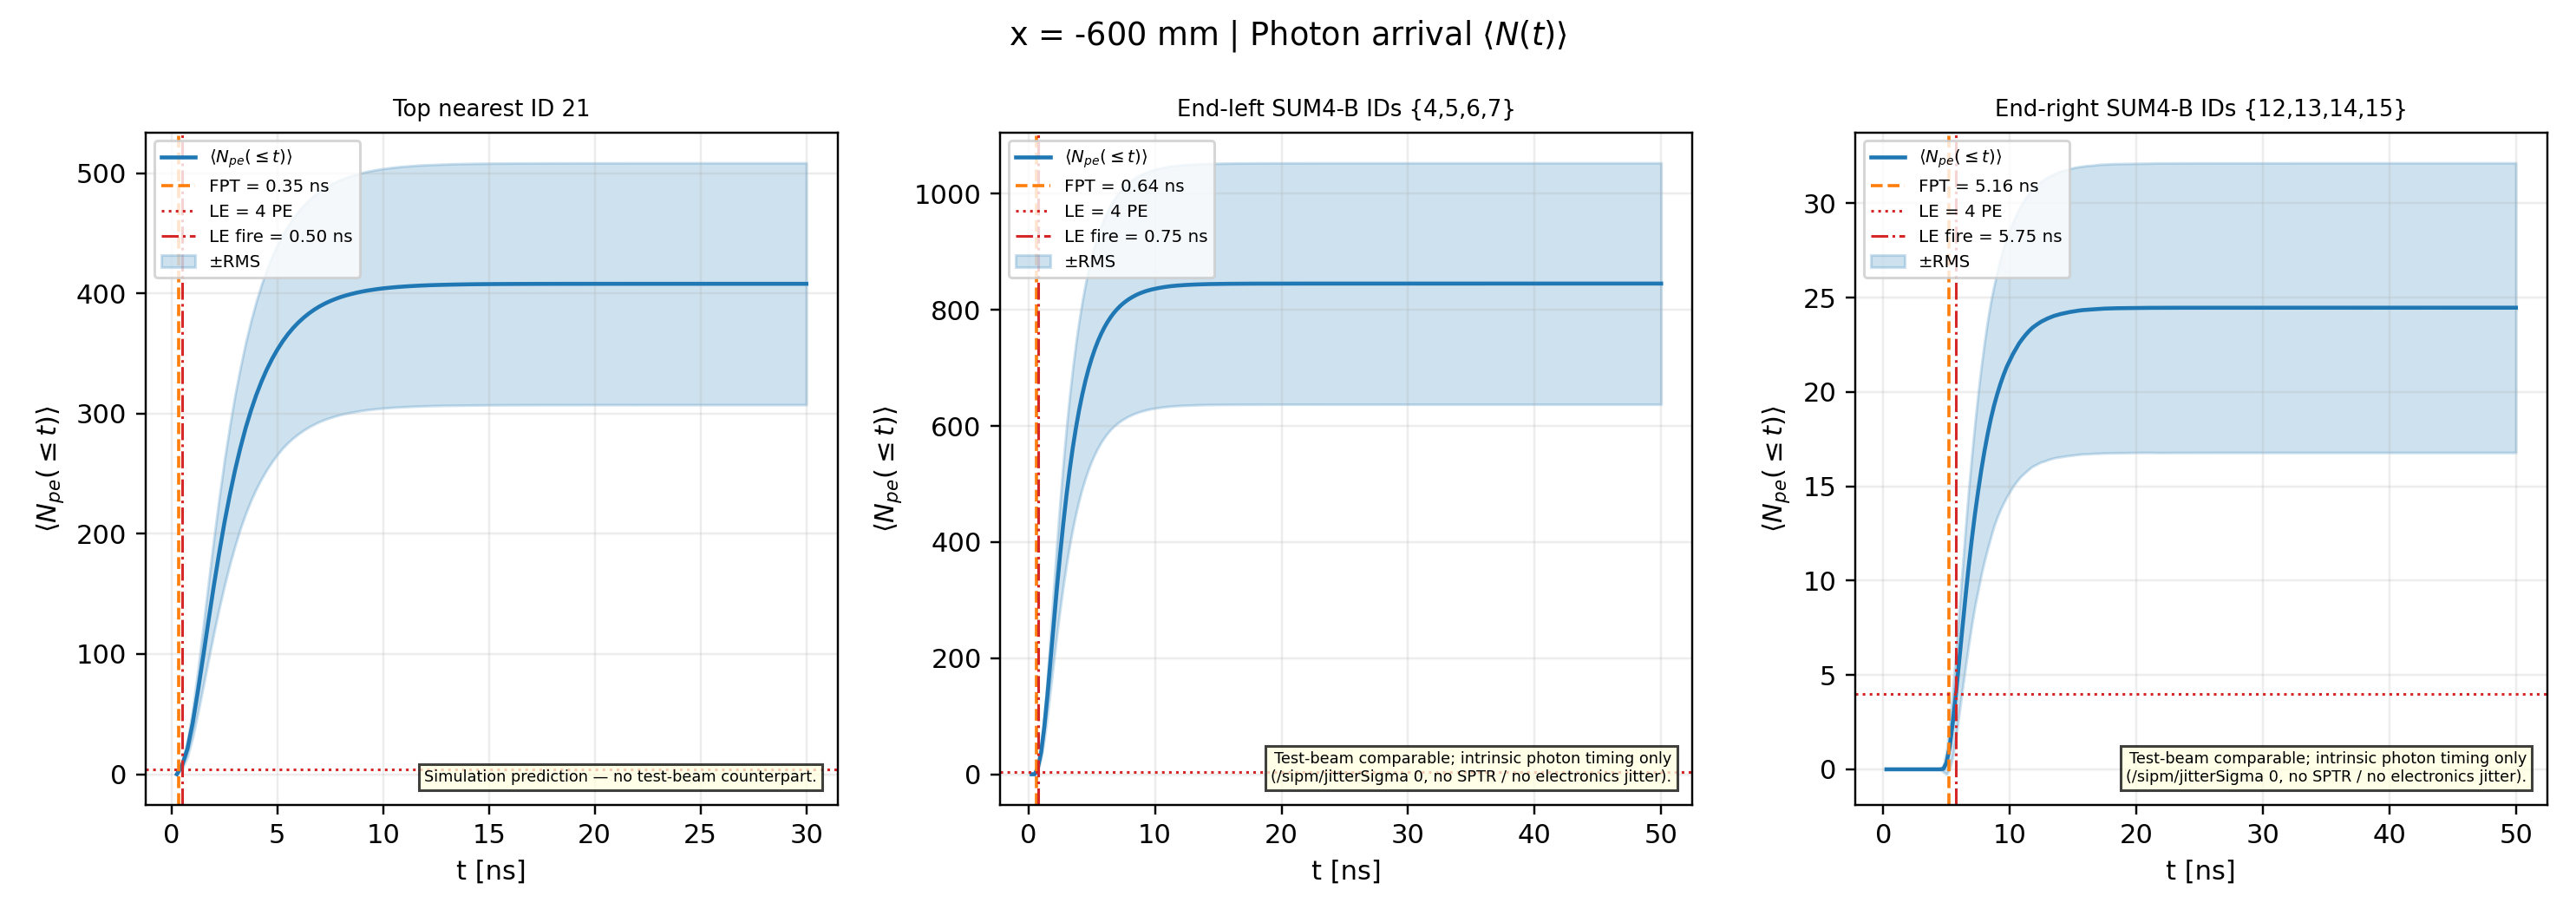
\includegraphics[width=\textwidth,height=0.78\textheight,keepaspectratio]{figs/exec11_arrival_-600mm.png}
\end{frame}
\begin{frame}{Position x=-550 mm}

\begin{columns}[T]
  \column{0.52\textwidth}
  
\includegraphics[width=\textwidth]{figs/muon_-550mm_geometry.png}
  \column{0.46\textwidth}
  
\includegraphics[width=\textwidth]{figs/muon_-550mm_top_profile.png}
  \tiny
  \begin{tabular}{lr}
    \toprule Quantity & Value \\ \midrule
    End L $N_{pe}$ & $1323.9\pm7.6$ \\
    End R $N_{pe}$ & $55.1\pm0.4$ \\
    Nearest Top ID & 23 (window-track exception) \\
    Nearest Top $N_{pe}$ & $352.9\pm2.1$ \\
    Nearest Top $\langle t\rangle$ &
      $2.7760\pm0.0023$ ns \\
    Nearest Top FPT & $0.34276\pm0.00025$ ns \\
    \bottomrule
  \end{tabular}
\end{columns}

\end{frame}
\begin{frame}{Run 5 $|$ x = -550 mm $|$ Photon arrival $\langle N(t)\rangle$}
\centering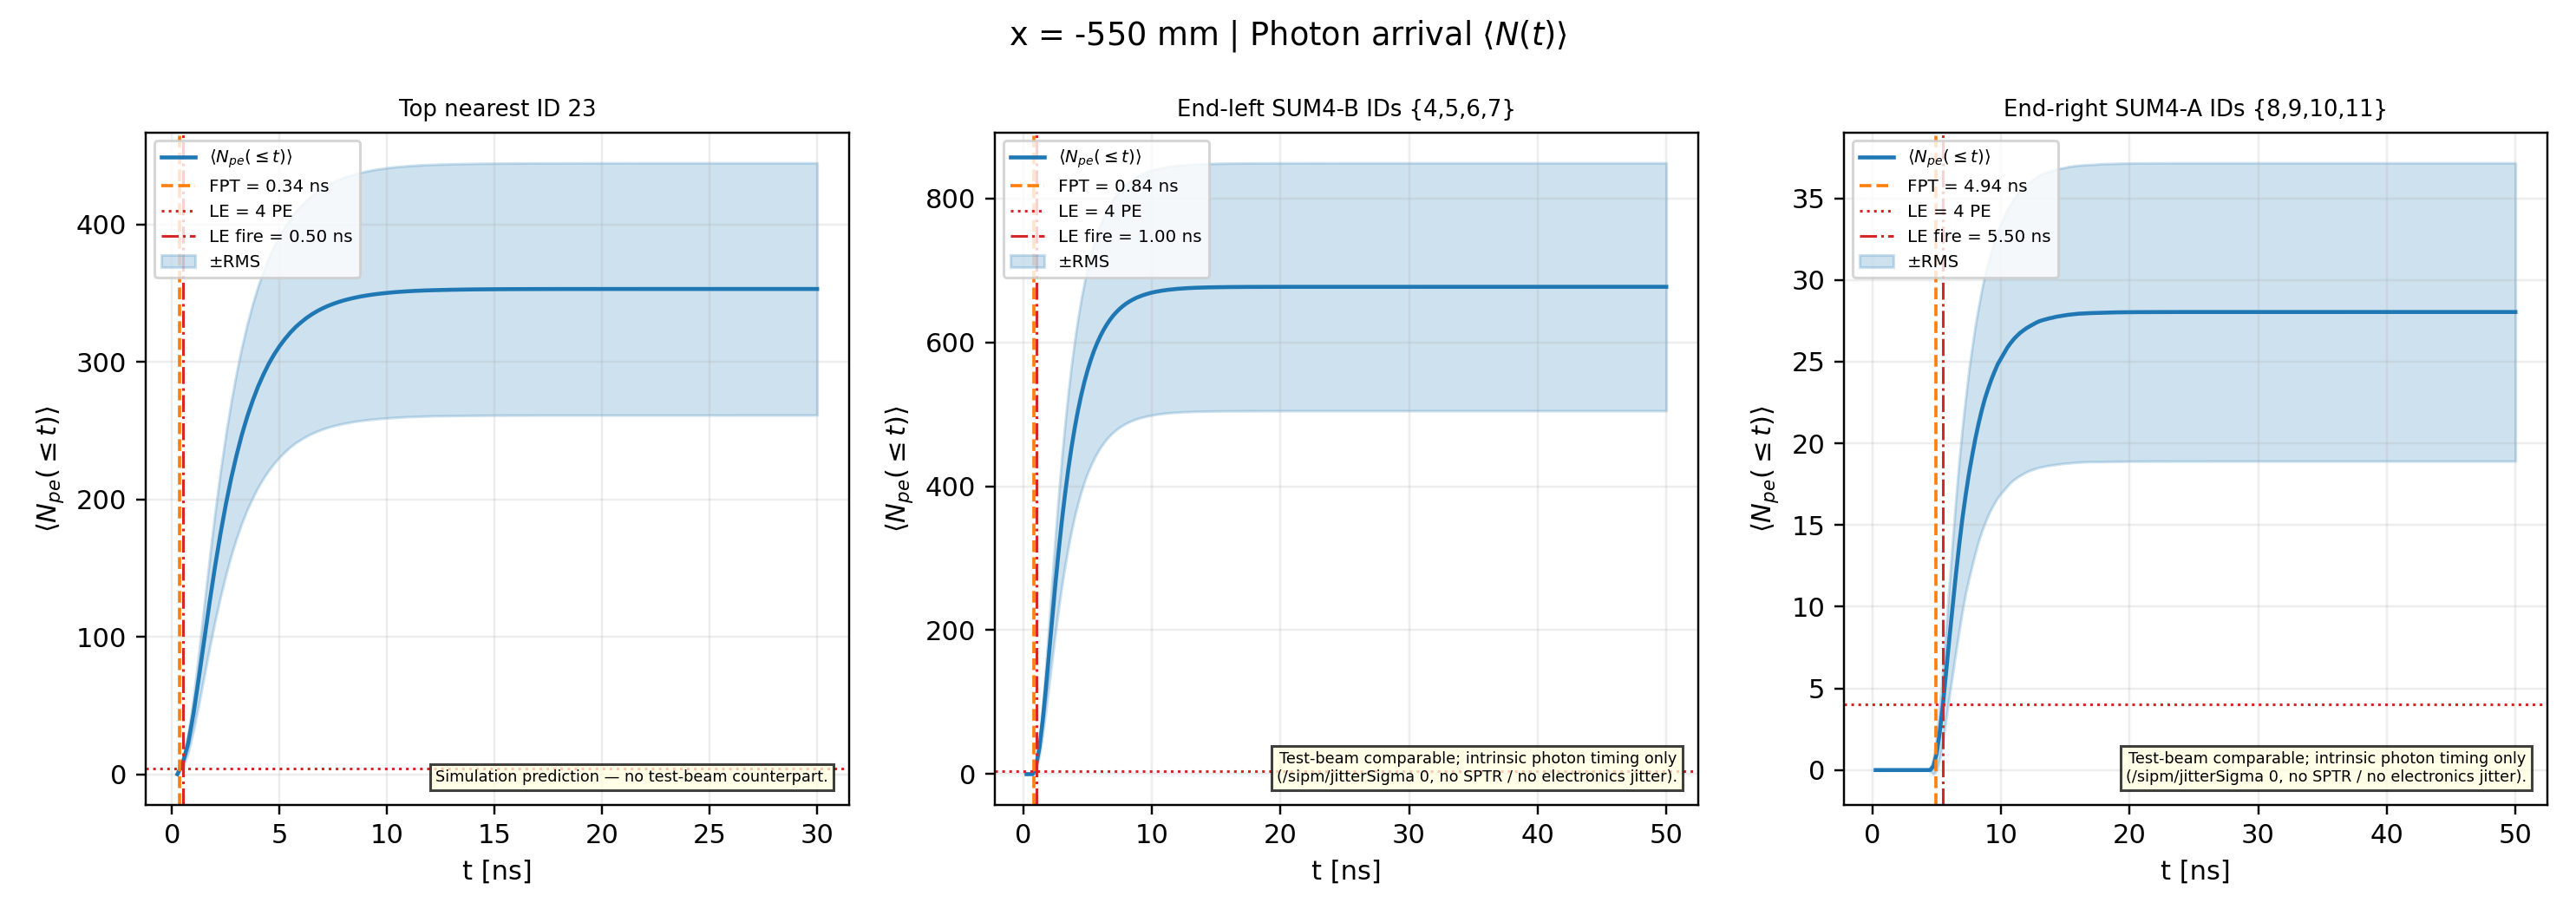
\includegraphics[width=\textwidth,height=0.78\textheight,keepaspectratio]{figs/exec11_arrival_-550mm.png}
\end{frame}
\begin{frame}{Position x=-500 mm}

\begin{columns}[T]
  \column{0.52\textwidth}
  
\includegraphics[width=\textwidth]{figs/muon_-500mm_geometry.png}
  \column{0.46\textwidth}
  
\includegraphics[width=\textwidth]{figs/muon_-500mm_top_profile.png}
  \tiny
  \begin{tabular}{lr}
    \toprule Quantity & Value \\ \midrule
    End L $N_{pe}$ & $1042.2\pm5.9$ \\
    End R $N_{pe}$ & $59.8\pm0.4$ \\
    Nearest Top ID & 26 (exact geometry) \\
    Nearest Top $N_{pe}$ & $410.9\pm2.3$ \\
    Nearest Top $\langle t\rangle$ &
      $2.9419\pm0.0022$ ns \\
    Nearest Top FPT & $0.34607\pm0.00023$ ns \\
    \bottomrule
  \end{tabular}
\end{columns}

\end{frame}
\begin{frame}{Run 6 $|$ x = -500 mm $|$ Photon arrival $\langle N(t)\rangle$}
\centering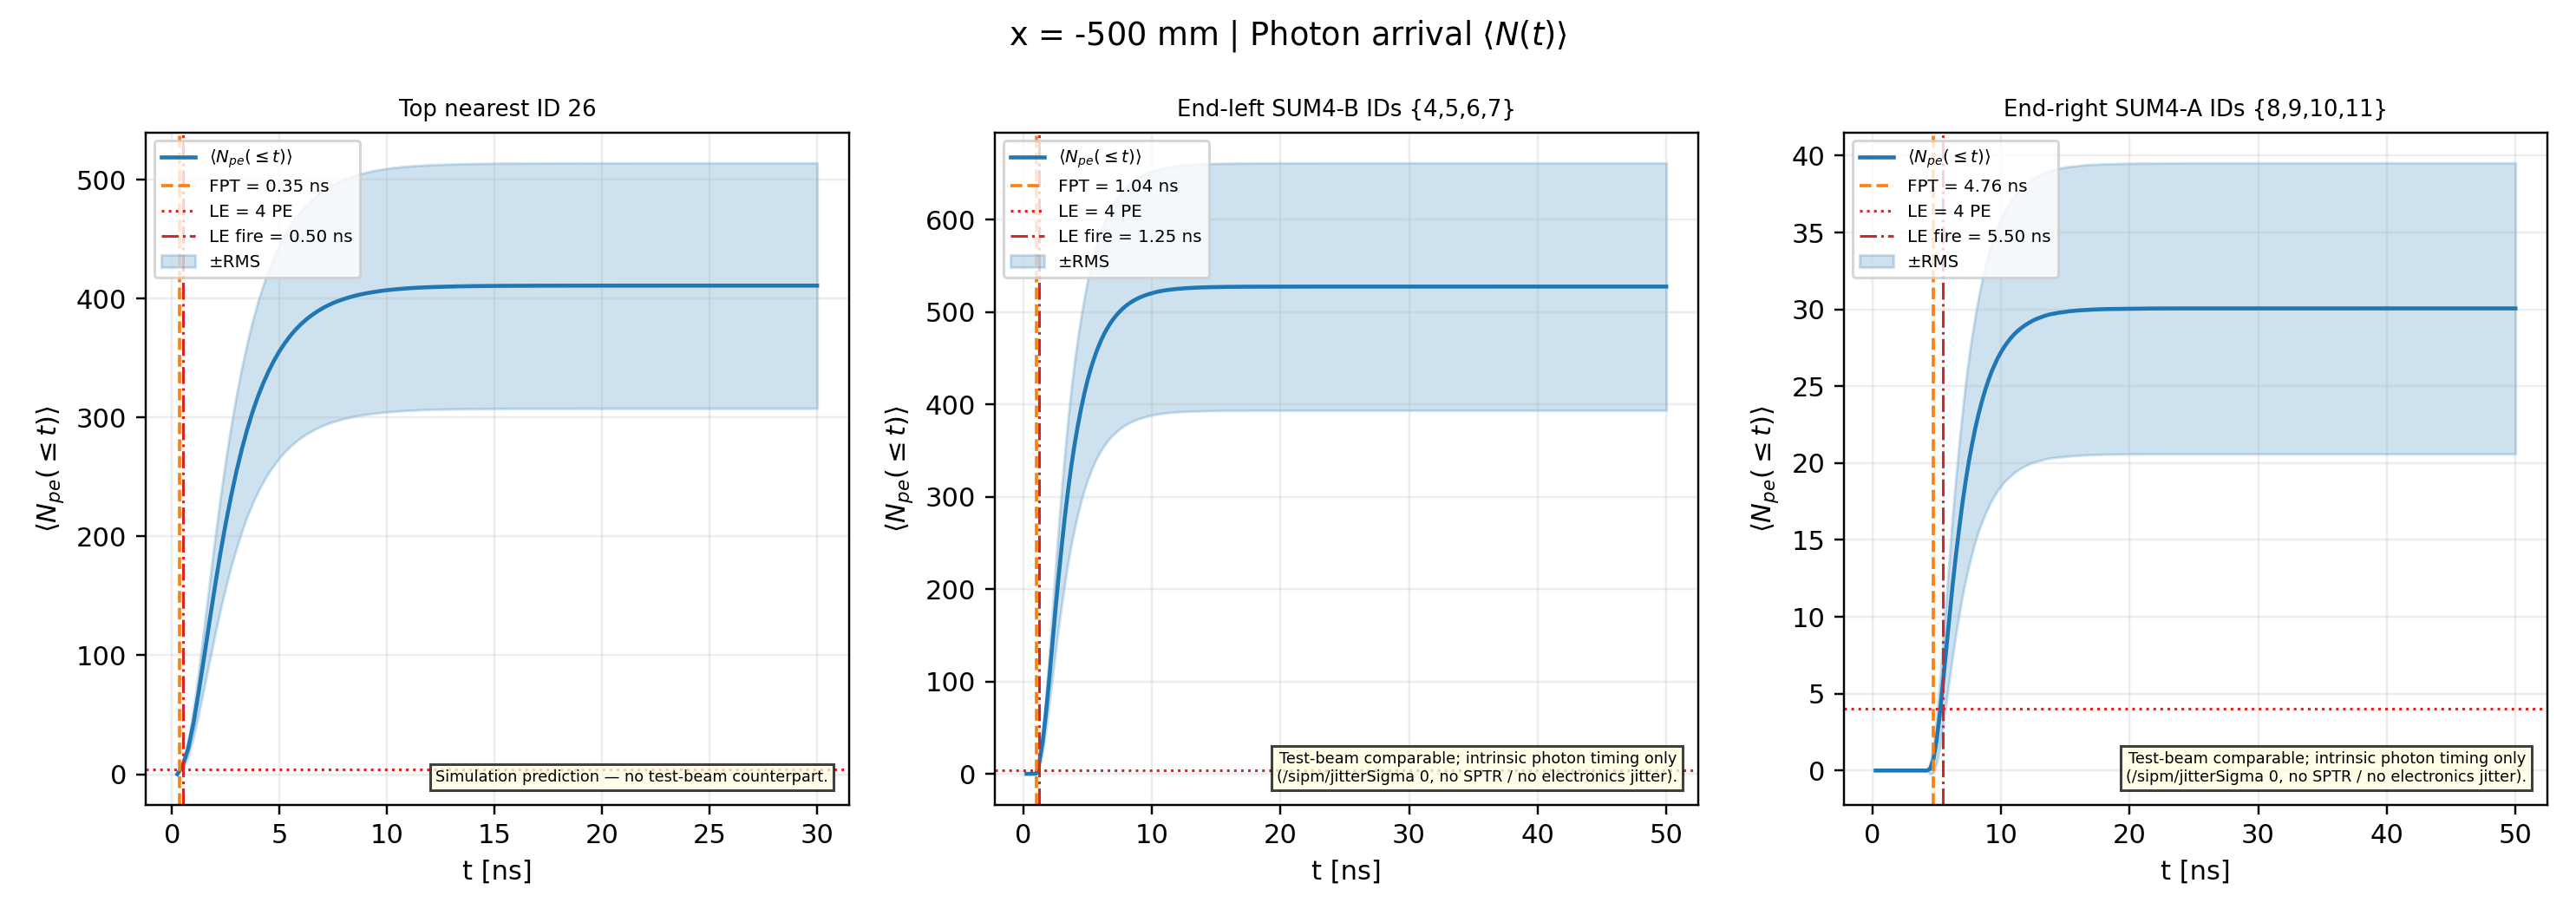
\includegraphics[width=\textwidth,height=0.78\textheight,keepaspectratio]{figs/exec11_arrival_-500mm.png}
\end{frame}
\begin{frame}{Position x=-450 mm}

\begin{columns}[T]
  \column{0.52\textwidth}
  
\includegraphics[width=\textwidth]{figs/muon_-450mm_geometry.png}
  \column{0.46\textwidth}
  
\includegraphics[width=\textwidth]{figs/muon_-450mm_top_profile.png}
  \tiny
  \begin{tabular}{lr}
    \toprule Quantity & Value \\ \midrule
    End L $N_{pe}$ & $832.9\pm4.2$ \\
    End R $N_{pe}$ & $65.8\pm0.4$ \\
    Nearest Top ID & 28 (window-track exception) \\
    Nearest Top $N_{pe}$ & $345.8\pm1.8$ \\
    Nearest Top $\langle t\rangle$ &
      $2.7793\pm0.0023$ ns \\
    Nearest Top FPT & $0.34237\pm0.00016$ ns \\
    \bottomrule
  \end{tabular}
\end{columns}

\end{frame}
\begin{frame}{Run 7 $|$ x = -450 mm $|$ Photon arrival $\langle N(t)\rangle$}
\centering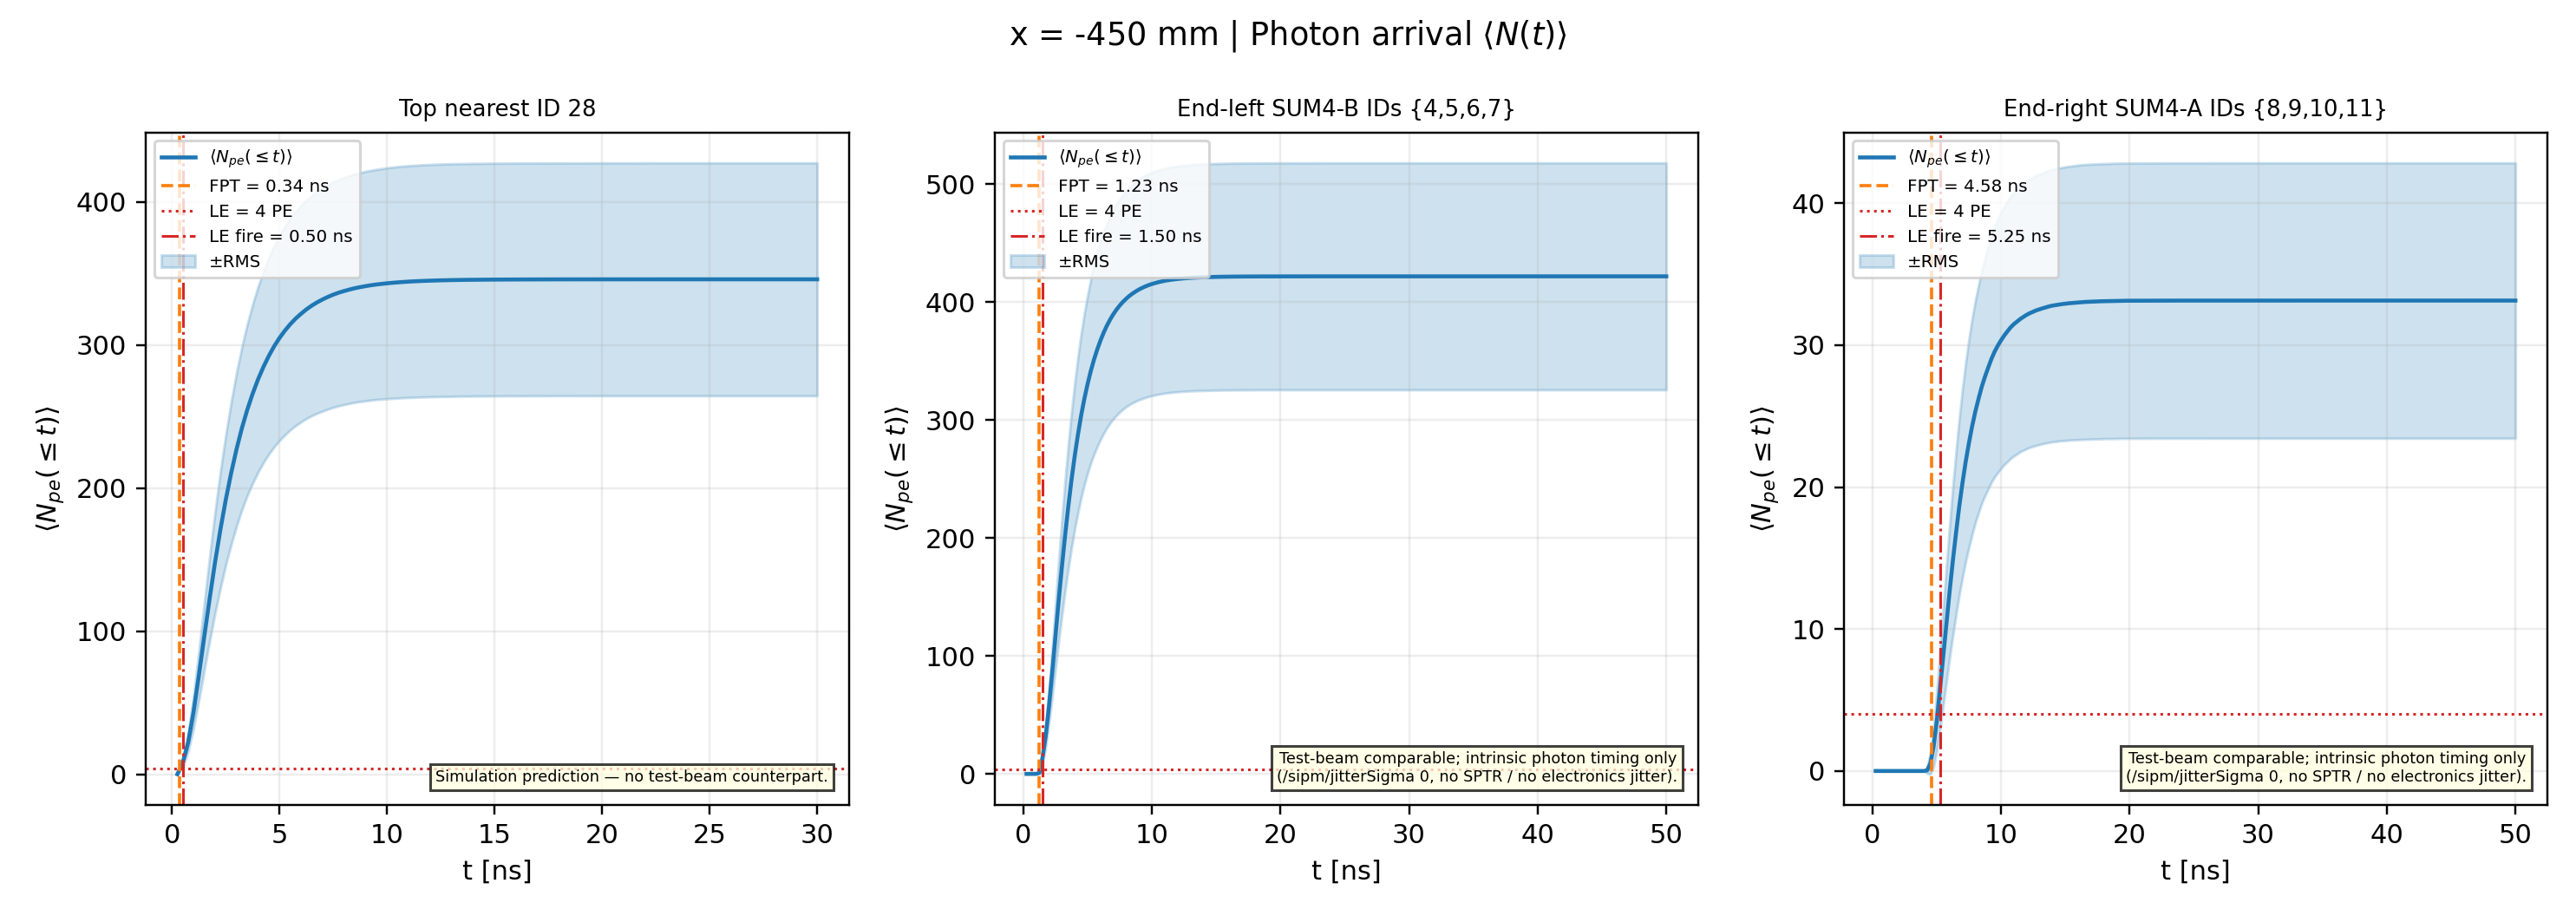
\includegraphics[width=\textwidth,height=0.78\textheight,keepaspectratio]{figs/exec11_arrival_-450mm.png}
\end{frame}
\begin{frame}{Position x=-400 mm}

\begin{columns}[T]
  \column{0.52\textwidth}
  
\includegraphics[width=\textwidth]{figs/muon_-400mm_geometry.png}
  \column{0.46\textwidth}
  
\includegraphics[width=\textwidth]{figs/muon_-400mm_top_profile.png}
  \tiny
  \begin{tabular}{lr}
    \toprule Quantity & Value \\ \midrule
    End L $N_{pe}$ & $691.3\pm3.9$ \\
    End R $N_{pe}$ & $74.5\pm0.5$ \\
    Nearest Top ID & 31 (exact geometry) \\
    Nearest Top $N_{pe}$ & $411.3\pm2.3$ \\
    Nearest Top $\langle t\rangle$ &
      $2.9399\pm0.0022$ ns \\
    Nearest Top FPT & $0.34597\pm0.00021$ ns \\
    \bottomrule
  \end{tabular}
\end{columns}

\end{frame}
\begin{frame}{Run 8 $|$ x = -400 mm $|$ Photon arrival $\langle N(t)\rangle$}
\centering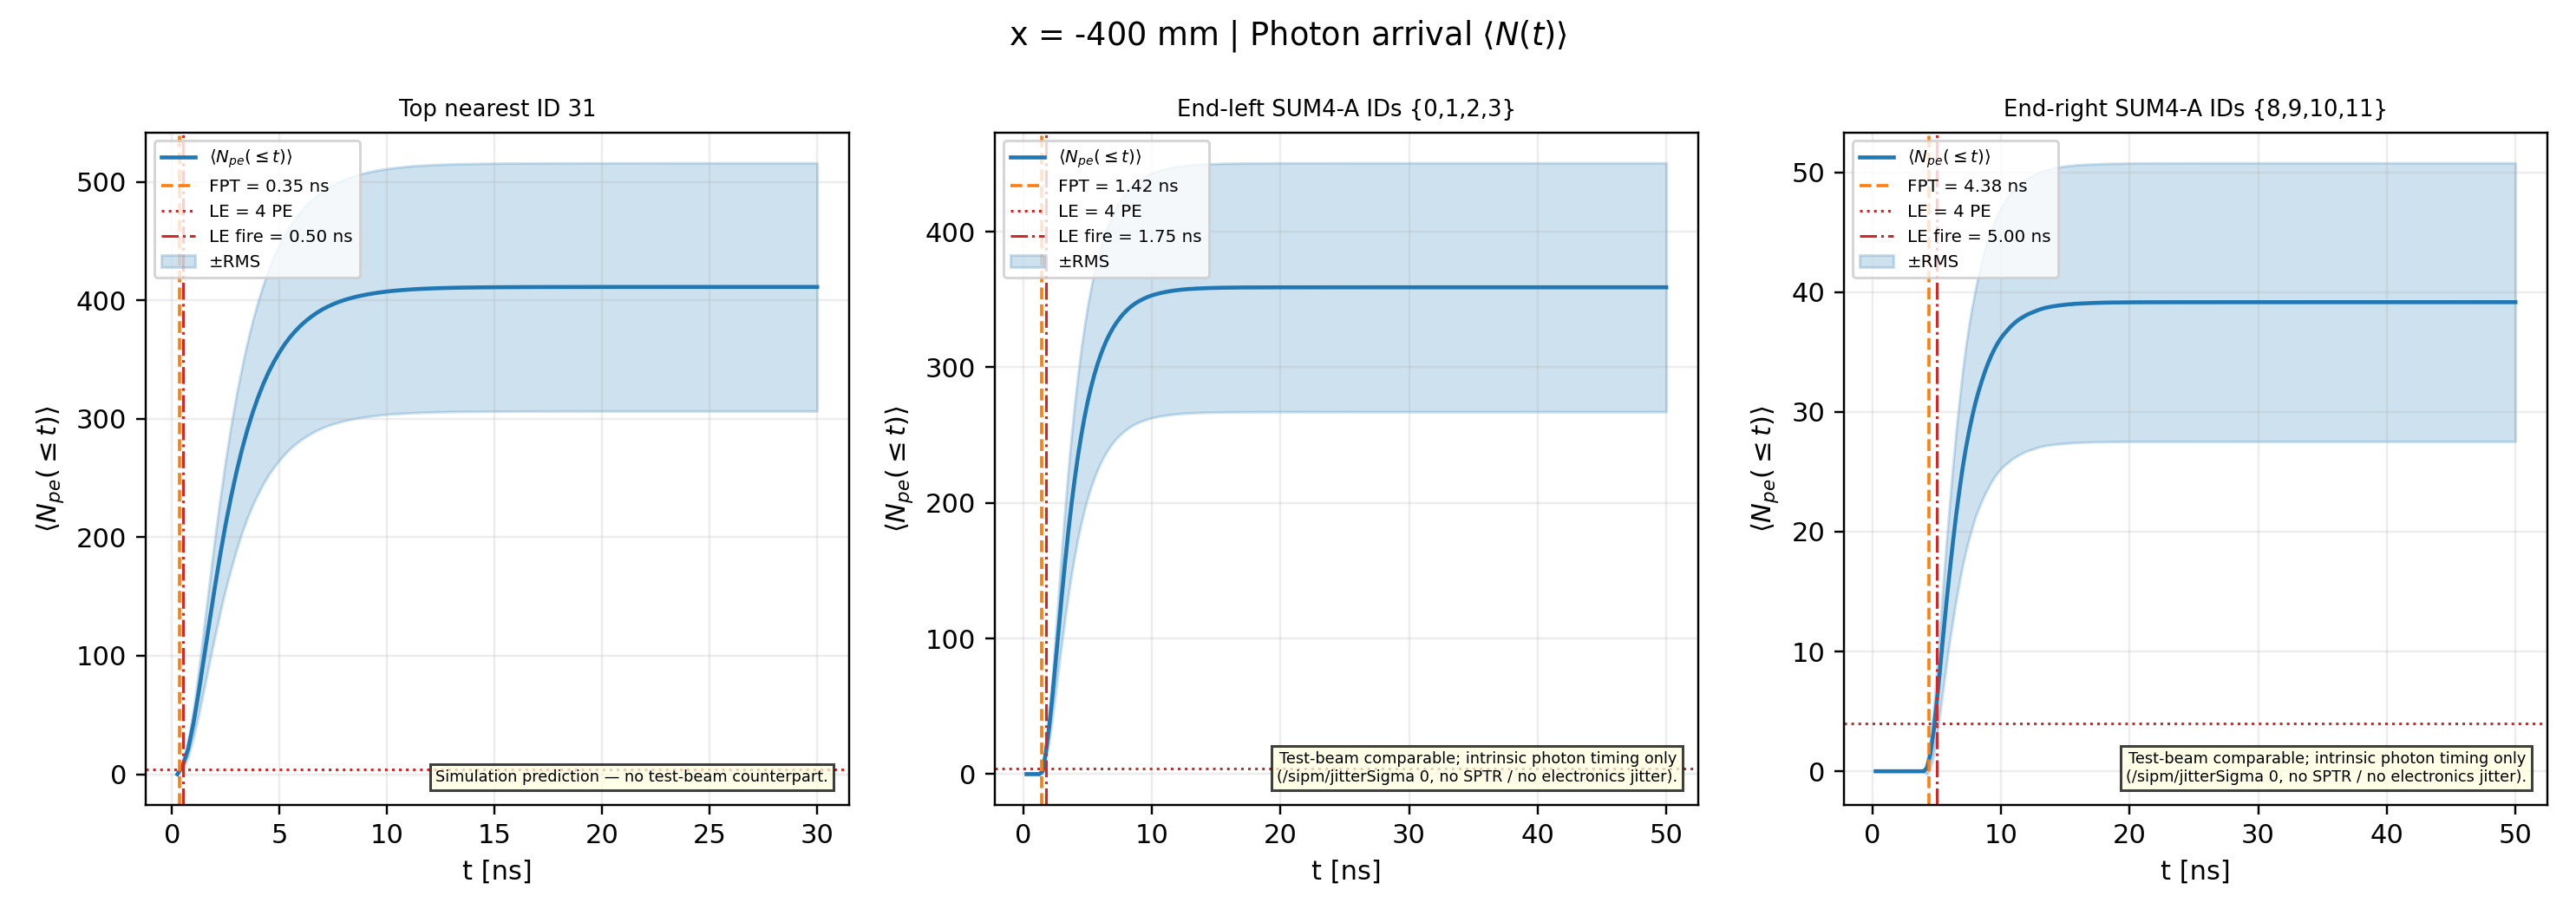
\includegraphics[width=\textwidth,height=0.78\textheight,keepaspectratio]{figs/exec11_arrival_-400mm.png}
\end{frame}
\begin{frame}{Position x=-350 mm}

\begin{columns}[T]
  \column{0.52\textwidth}
  
\includegraphics[width=\textwidth]{figs/muon_-350mm_geometry.png}
  \column{0.46\textwidth}
  
\includegraphics[width=\textwidth]{figs/muon_-350mm_top_profile.png}
  \tiny
  \begin{tabular}{lr}
    \toprule Quantity & Value \\ \midrule
    End L $N_{pe}$ & $575.0\pm3.1$ \\
    End R $N_{pe}$ & $84.1\pm0.5$ \\
    Nearest Top ID & 33 (window-track exception) \\
    Nearest Top $N_{pe}$ & $349.3\pm1.9$ \\
    Nearest Top $\langle t\rangle$ &
      $2.7748\pm0.0023$ ns \\
    Nearest Top FPT & $0.34234\pm0.00015$ ns \\
    \bottomrule
  \end{tabular}
\end{columns}

\end{frame}
\begin{frame}{Run 9 $|$ x = -350 mm $|$ Photon arrival $\langle N(t)\rangle$}
\centering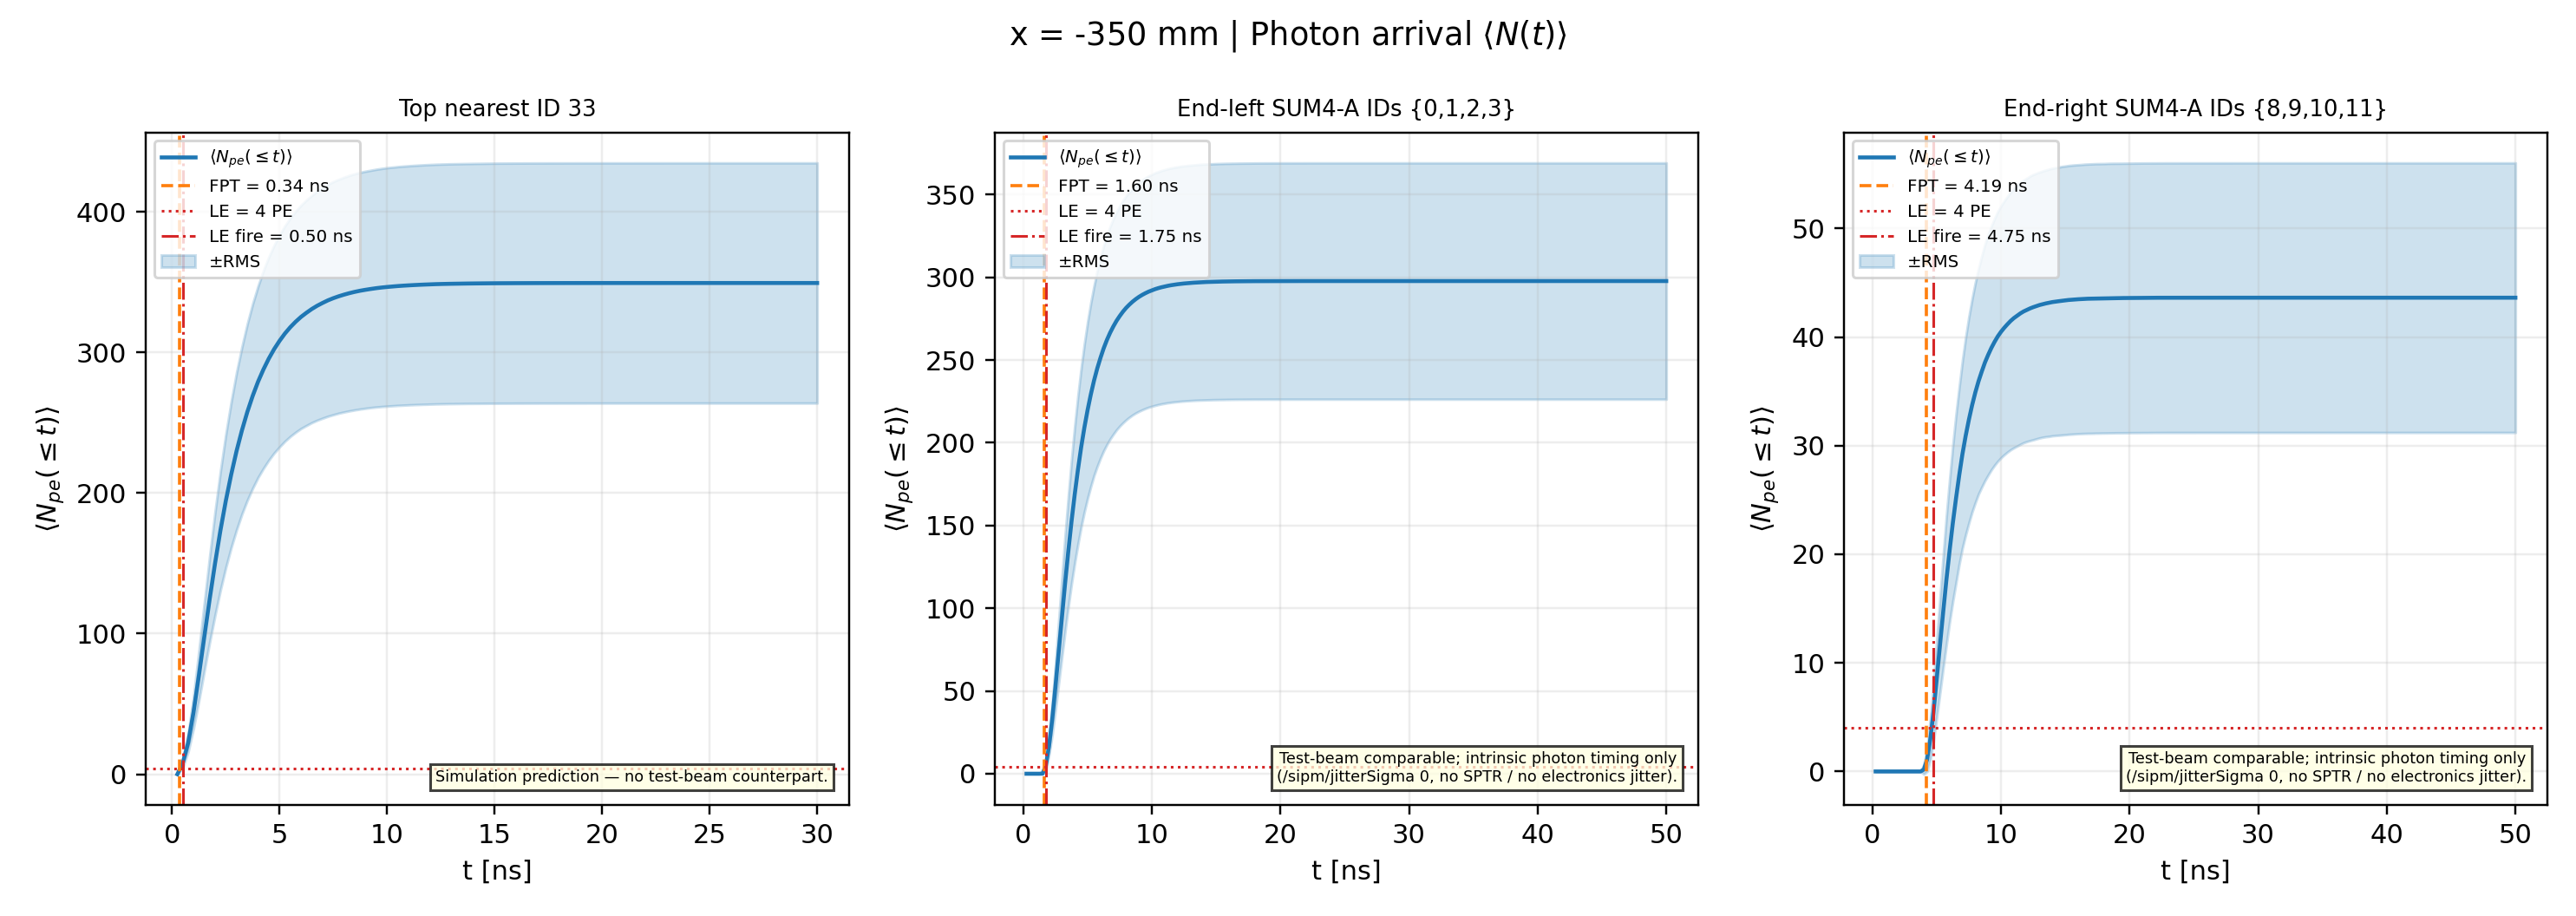
\includegraphics[width=\textwidth,height=0.78\textheight,keepaspectratio]{figs/exec11_arrival_-350mm.png}
\end{frame}
\begin{frame}{Position x=-300 mm}

\begin{columns}[T]
  \column{0.52\textwidth}
  
\includegraphics[width=\textwidth]{figs/muon_-300mm_geometry.png}
  \column{0.46\textwidth}
  
\includegraphics[width=\textwidth]{figs/muon_-300mm_top_profile.png}
  \tiny
  \begin{tabular}{lr}
    \toprule Quantity & Value \\ \midrule
    End L $N_{pe}$ & $482.3\pm2.8$ \\
    End R $N_{pe}$ & $94.2\pm0.6$ \\
    Nearest Top ID & 36 (exact geometry) \\
    Nearest Top $N_{pe}$ & $413.7\pm2.5$ \\
    Nearest Top $\langle t\rangle$ &
      $2.9387\pm0.0022$ ns \\
    Nearest Top FPT & $0.34593\pm0.00023$ ns \\
    \bottomrule
  \end{tabular}
\end{columns}

\end{frame}
\begin{frame}{Run 10 $|$ x = -300 mm $|$ Photon arrival $\langle N(t)\rangle$}
\centering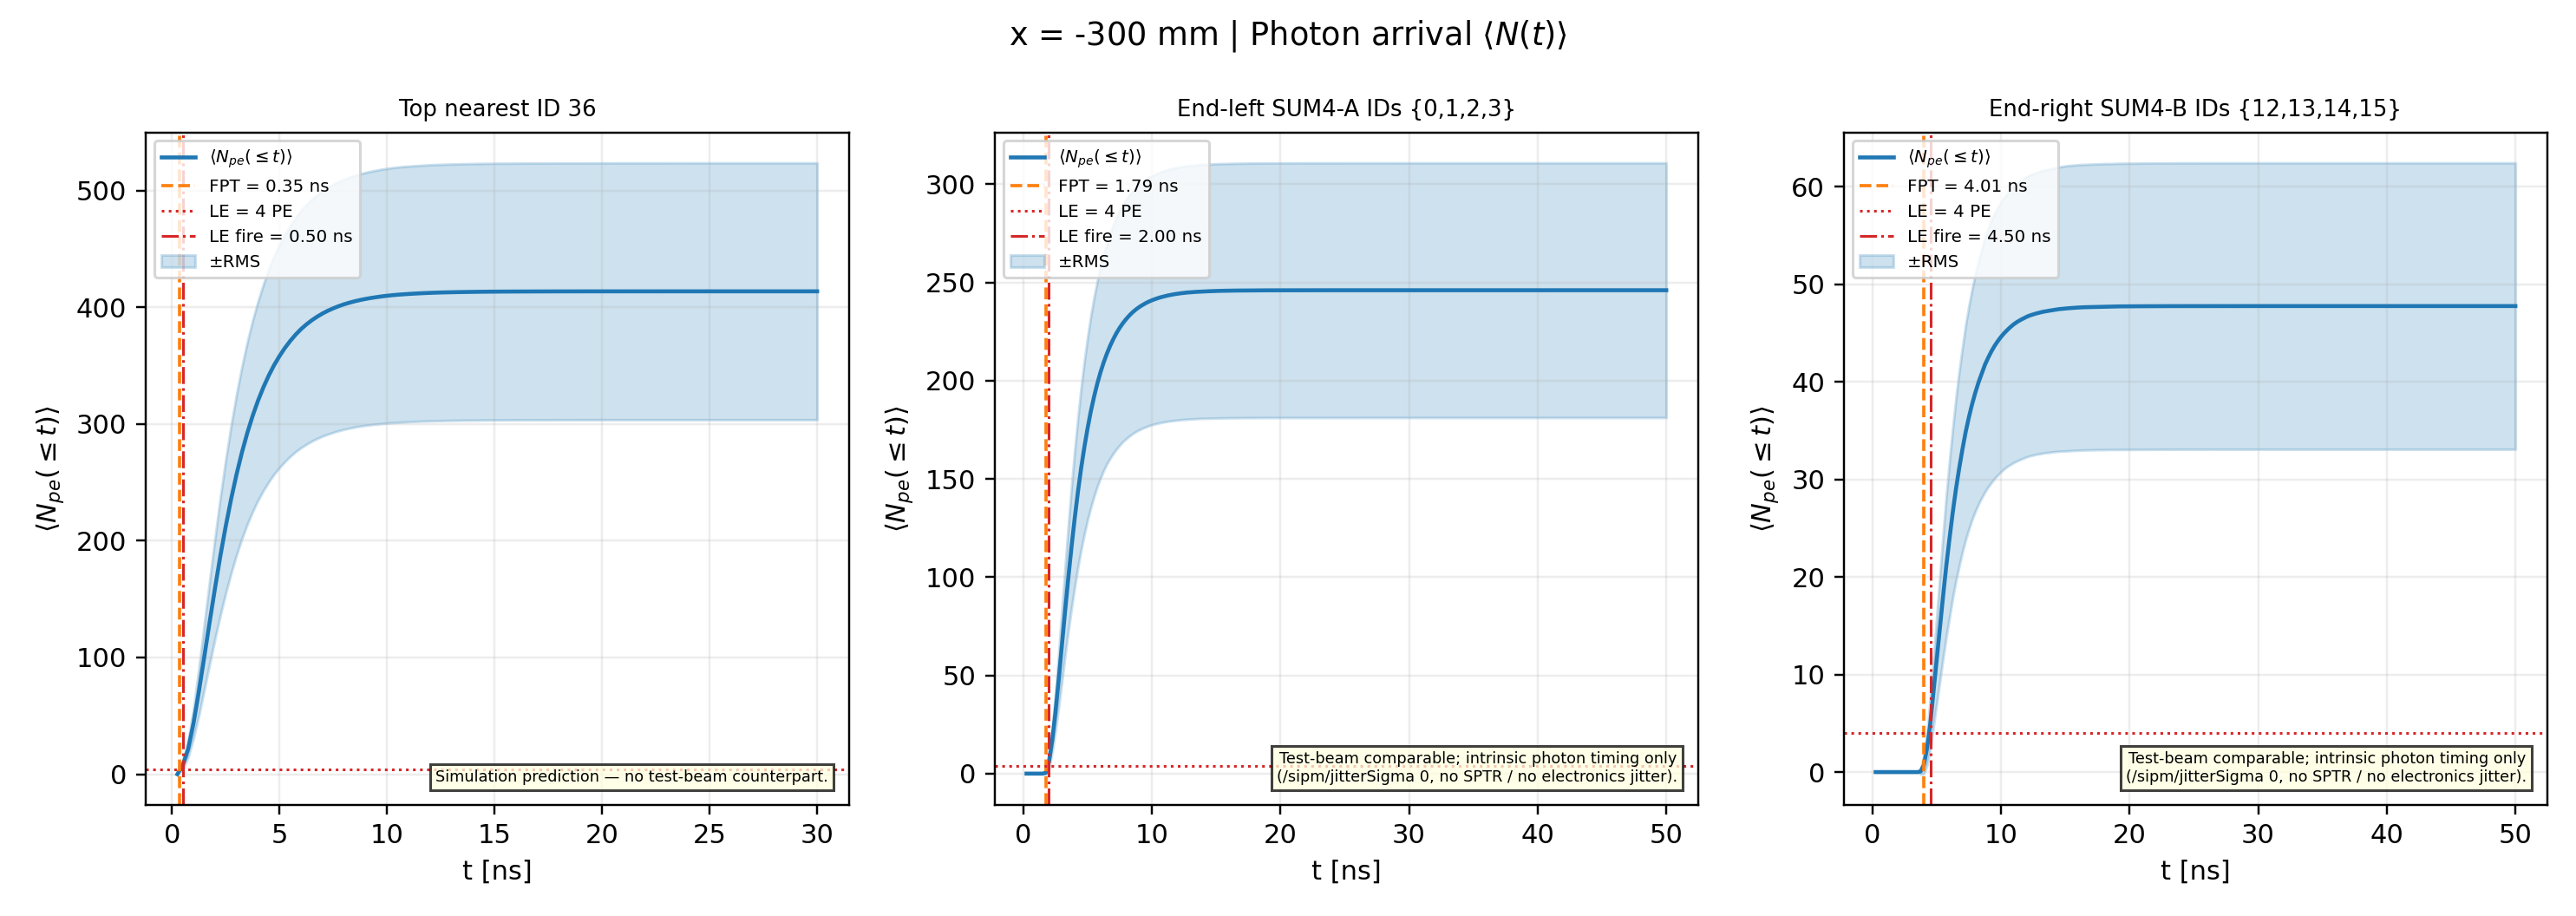
\includegraphics[width=\textwidth,height=0.78\textheight,keepaspectratio]{figs/exec11_arrival_-300mm.png}
\end{frame}
\begin{frame}{Position x=-250 mm}

\begin{columns}[T]
  \column{0.52\textwidth}
  
\includegraphics[width=\textwidth]{figs/muon_-250mm_geometry.png}
  \column{0.46\textwidth}
  
\includegraphics[width=\textwidth]{figs/muon_-250mm_top_profile.png}
  \tiny
  \begin{tabular}{lr}
    \toprule Quantity & Value \\ \midrule
    End L $N_{pe}$ & $415.8\pm2.4$ \\
    End R $N_{pe}$ & $105.5\pm0.7$ \\
    Nearest Top ID & 38 (window-track exception) \\
    Nearest Top $N_{pe}$ & $352.2\pm2.1$ \\
    Nearest Top $\langle t\rangle$ &
      $2.7758\pm0.0023$ ns \\
    Nearest Top FPT & $0.34224\pm0.00013$ ns \\
    \bottomrule
  \end{tabular}
\end{columns}

\end{frame}
\begin{frame}{Run 11 $|$ x = -250 mm $|$ Photon arrival $\langle N(t)\rangle$}
\centering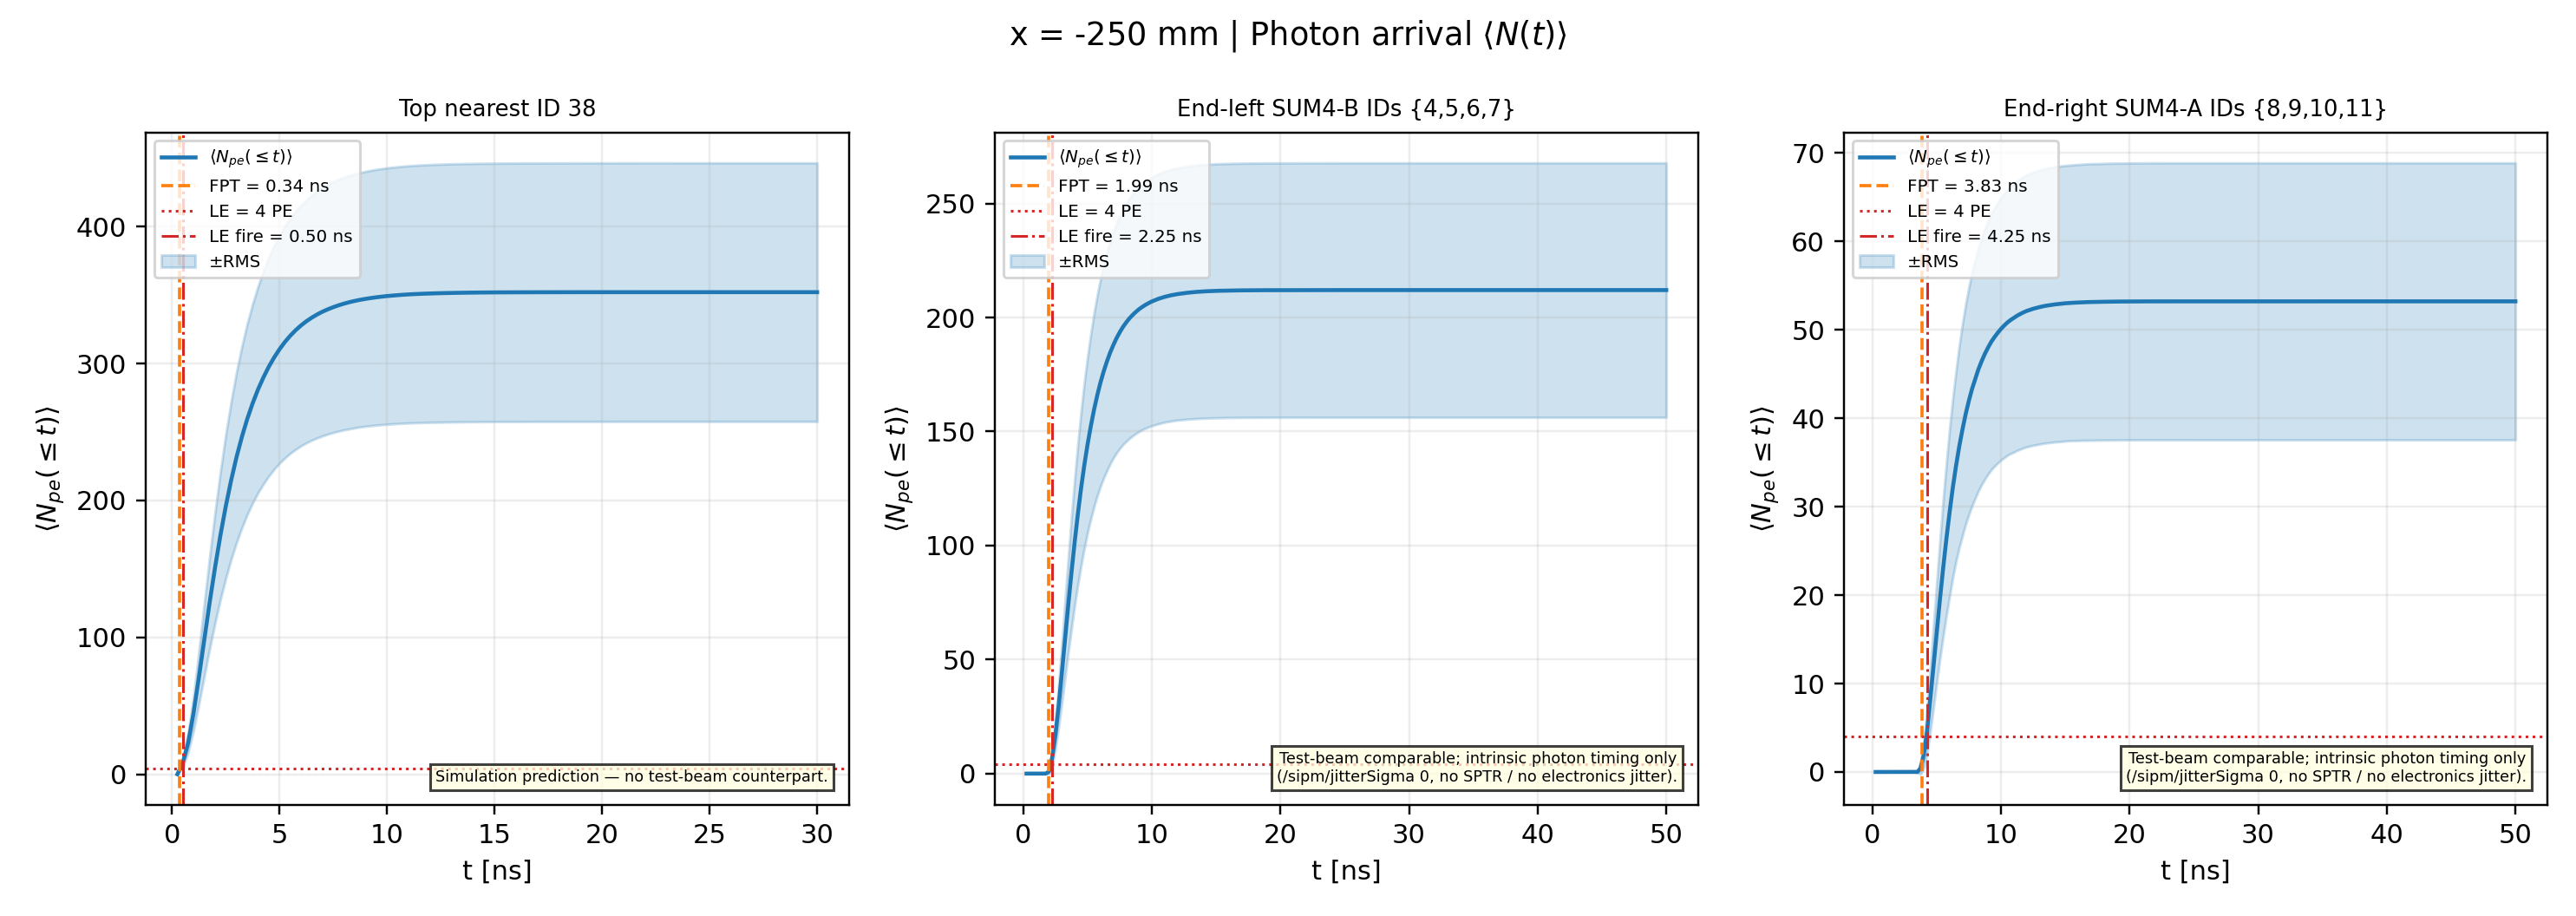
\includegraphics[width=\textwidth,height=0.78\textheight,keepaspectratio]{figs/exec11_arrival_-250mm.png}
\end{frame}
\begin{frame}{Position x=-200 mm}

\begin{columns}[T]
  \column{0.52\textwidth}
  
\includegraphics[width=\textwidth]{figs/muon_-200mm_geometry.png}
  \column{0.46\textwidth}
  
\includegraphics[width=\textwidth]{figs/muon_-200mm_top_profile.png}
  \tiny
  \begin{tabular}{lr}
    \toprule Quantity & Value \\ \midrule
    End L $N_{pe}$ & $353.5\pm2.0$ \\
    End R $N_{pe}$ & $118.4\pm0.7$ \\
    Nearest Top ID & 41 (exact geometry) \\
    Nearest Top $N_{pe}$ & $412.5\pm2.3$ \\
    Nearest Top $\langle t\rangle$ &
      $2.9407\pm0.0022$ ns \\
    Nearest Top FPT & $0.34577\pm0.00020$ ns \\
    \bottomrule
  \end{tabular}
\end{columns}

\end{frame}
\begin{frame}{Run 12 $|$ x = -200 mm $|$ Photon arrival $\langle N(t)\rangle$}
\centering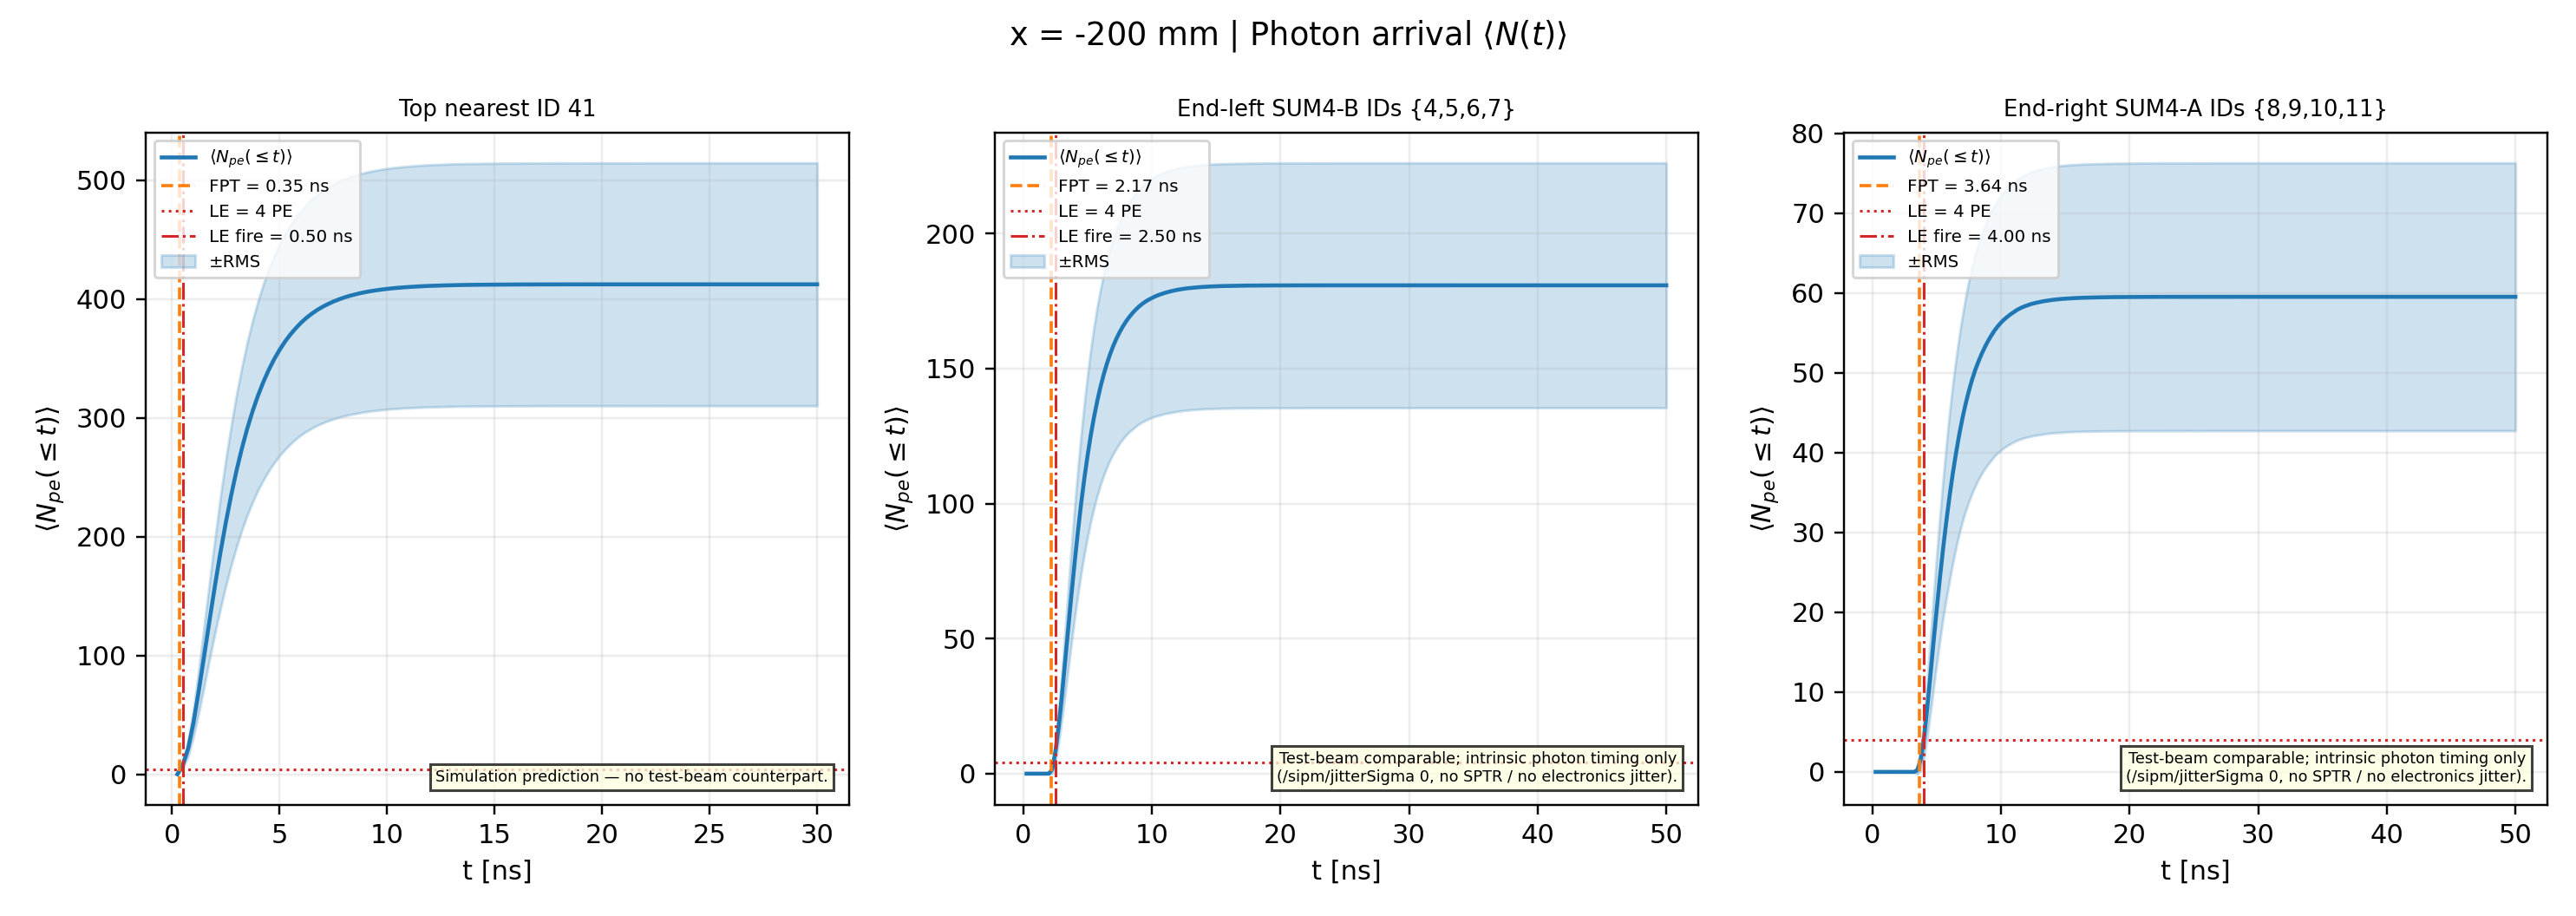
\includegraphics[width=\textwidth,height=0.78\textheight,keepaspectratio]{figs/exec11_arrival_-200mm.png}
\end{frame}
\begin{frame}{Position x=-150 mm}

\begin{columns}[T]
  \column{0.52\textwidth}
  
\includegraphics[width=\textwidth]{figs/muon_-150mm_geometry.png}
  \column{0.46\textwidth}
  
\includegraphics[width=\textwidth]{figs/muon_-150mm_top_profile.png}
  \tiny
  \begin{tabular}{lr}
    \toprule Quantity & Value \\ \midrule
    End L $N_{pe}$ & $302.1\pm1.8$ \\
    End R $N_{pe}$ & $134.7\pm0.8$ \\
    Nearest Top ID & 43 (window-track exception) \\
    Nearest Top $N_{pe}$ & $350.8\pm2.1$ \\
    Nearest Top $\langle t\rangle$ &
      $2.7749\pm0.0023$ ns \\
    Nearest Top FPT & $0.34232\pm0.00017$ ns \\
    \bottomrule
  \end{tabular}
\end{columns}

\end{frame}
\begin{frame}{Run 13 $|$ x = -150 mm $|$ Photon arrival $\langle N(t)\rangle$}
\centering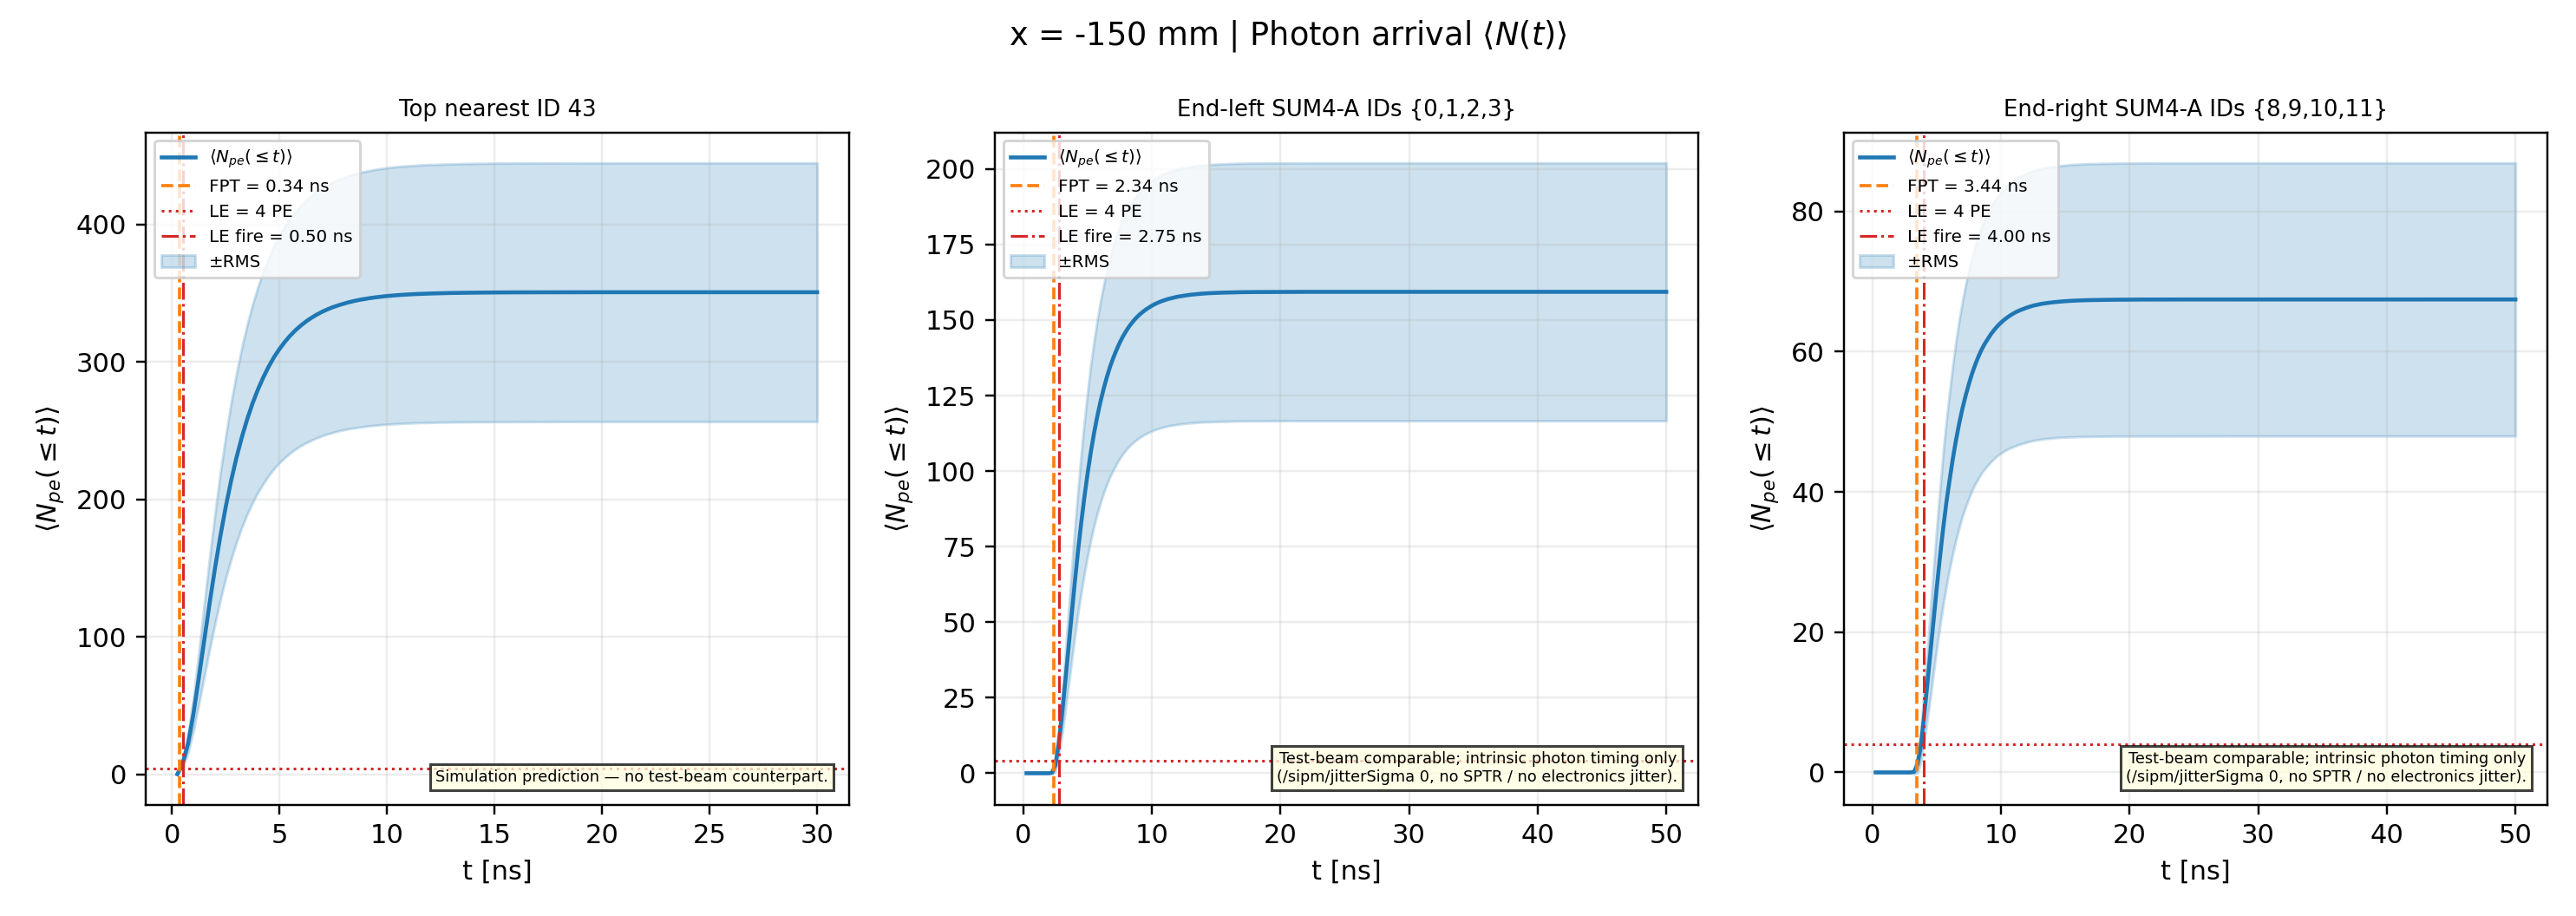
\includegraphics[width=\textwidth,height=0.78\textheight,keepaspectratio]{figs/exec11_arrival_-150mm.png}
\end{frame}
\begin{frame}{Position x=-100 mm}

\begin{columns}[T]
  \column{0.52\textwidth}
  
\includegraphics[width=\textwidth]{figs/muon_-100mm_geometry.png}
  \column{0.46\textwidth}
  
\includegraphics[width=\textwidth]{figs/muon_-100mm_top_profile.png}
  \tiny
  \begin{tabular}{lr}
    \toprule Quantity & Value \\ \midrule
    End L $N_{pe}$ & $256.3\pm1.5$ \\
    End R $N_{pe}$ & $151.4\pm0.9$ \\
    Nearest Top ID & 46 (exact geometry) \\
    Nearest Top $N_{pe}$ & $411.0\pm2.3$ \\
    Nearest Top $\langle t\rangle$ &
      $2.9426\pm0.0022$ ns \\
    Nearest Top FPT & $0.34620\pm0.00024$ ns \\
    \bottomrule
  \end{tabular}
\end{columns}

\end{frame}
\begin{frame}{Run 14 $|$ x = -100 mm $|$ Photon arrival $\langle N(t)\rangle$}
\centering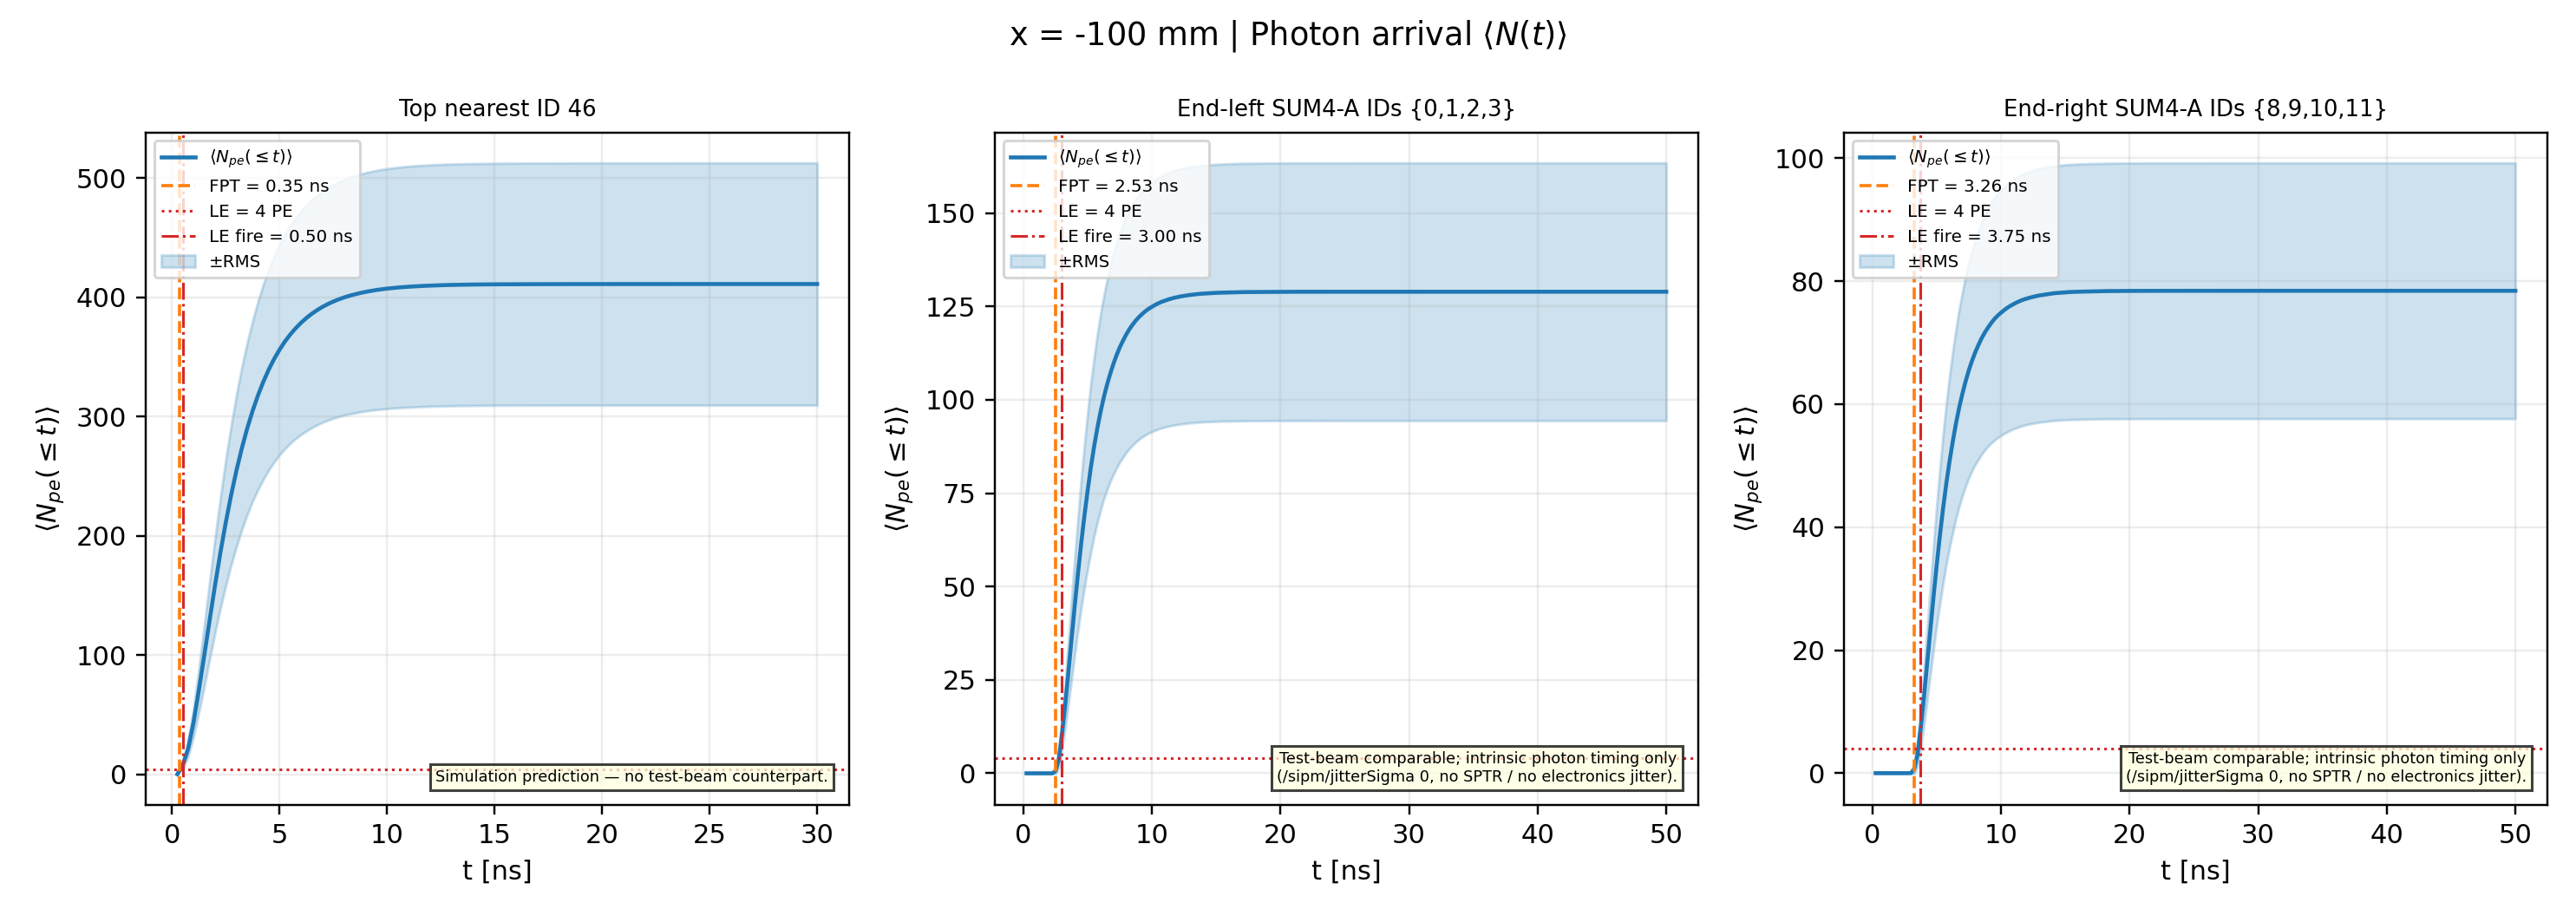
\includegraphics[width=\textwidth,height=0.78\textheight,keepaspectratio]{figs/exec11_arrival_-100mm.png}
\end{frame}
\begin{frame}{Position x=-50 mm}

\begin{columns}[T]
  \column{0.52\textwidth}
  
\includegraphics[width=\textwidth]{figs/muon_-50mm_geometry.png}
  \column{0.46\textwidth}
  
\includegraphics[width=\textwidth]{figs/muon_-50mm_top_profile.png}
  \tiny
  \begin{tabular}{lr}
    \toprule Quantity & Value \\ \midrule
    End L $N_{pe}$ & $226.7\pm1.4$ \\
    End R $N_{pe}$ & $172.7\pm1.1$ \\
    Nearest Top ID & 48 (window-track exception) \\
    Nearest Top $N_{pe}$ & $352.0\pm2.1$ \\
    Nearest Top $\langle t\rangle$ &
      $2.7740\pm0.0023$ ns \\
    Nearest Top FPT & $0.34228\pm0.00018$ ns \\
    \bottomrule
  \end{tabular}
\end{columns}

\end{frame}
\begin{frame}{Run 15 $|$ x = -50 mm $|$ Photon arrival $\langle N(t)\rangle$}
\centering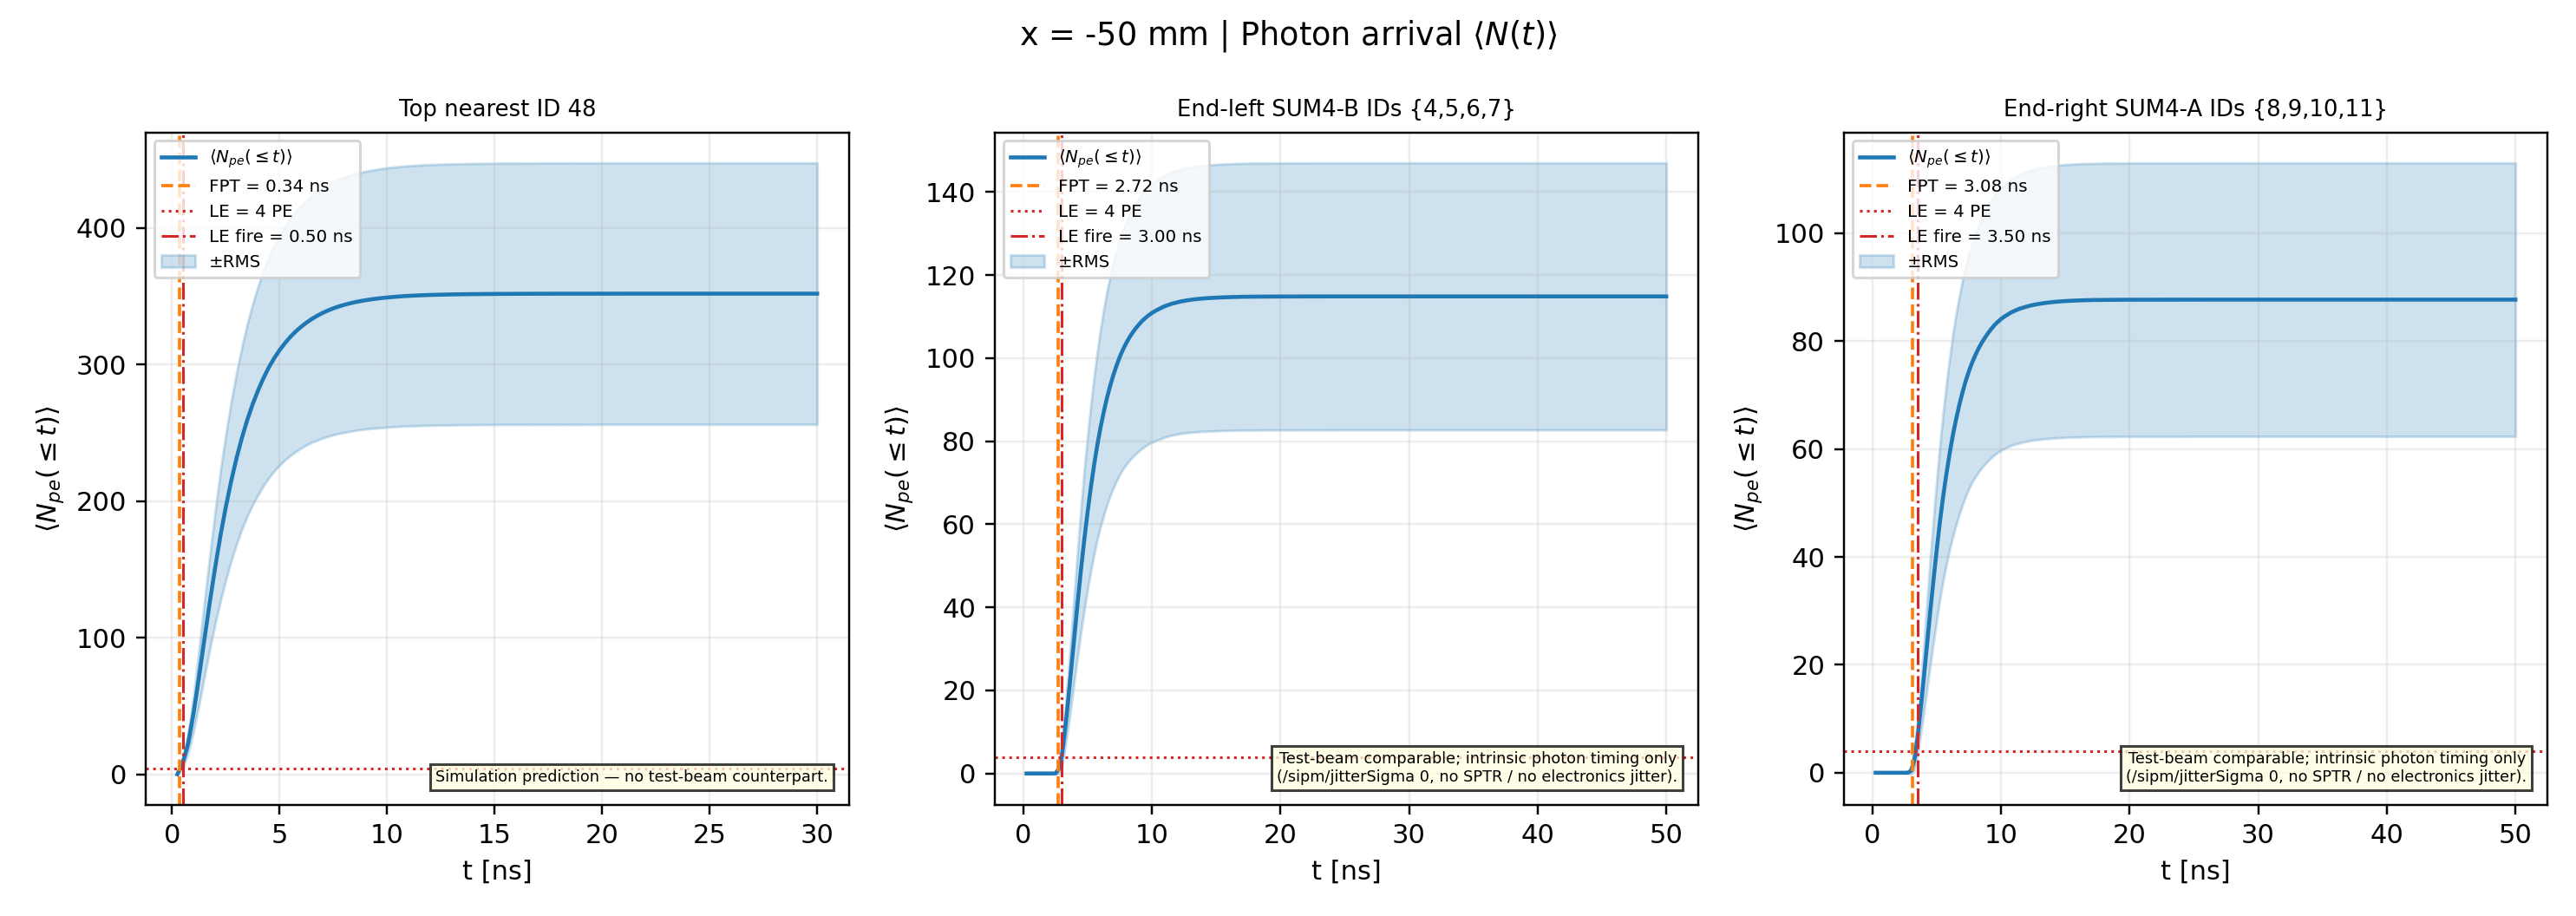
\includegraphics[width=\textwidth,height=0.78\textheight,keepaspectratio]{figs/exec11_arrival_-50mm.png}
\end{frame}
\begin{frame}{Position x=0 mm}

\begin{columns}[T]
  \column{0.52\textwidth}
  
\includegraphics[width=\textwidth]{figs/muon_0mm_geometry.png}
  \column{0.46\textwidth}
  
\includegraphics[width=\textwidth]{figs/muon_0mm_top_profile.png}
  \tiny
  \begin{tabular}{lr}
    \toprule Quantity & Value \\ \midrule
    End L $N_{pe}$ & $194.4\pm1.1$ \\
    End R $N_{pe}$ & $195.2\pm1.1$ \\
    Nearest Top ID & 51 (exact geometry) \\
    Nearest Top $N_{pe}$ & $407.3\pm2.2$ \\
    Nearest Top $\langle t\rangle$ &
      $3.0030\pm0.0022$ ns \\
    Nearest Top FPT & $0.35075\pm0.00020$ ns \\
    \bottomrule
  \end{tabular}
\end{columns}

\end{frame}
\begin{frame}{Run 16 $|$ x = +0 mm $|$ Photon arrival $\langle N(t)\rangle$}
\centering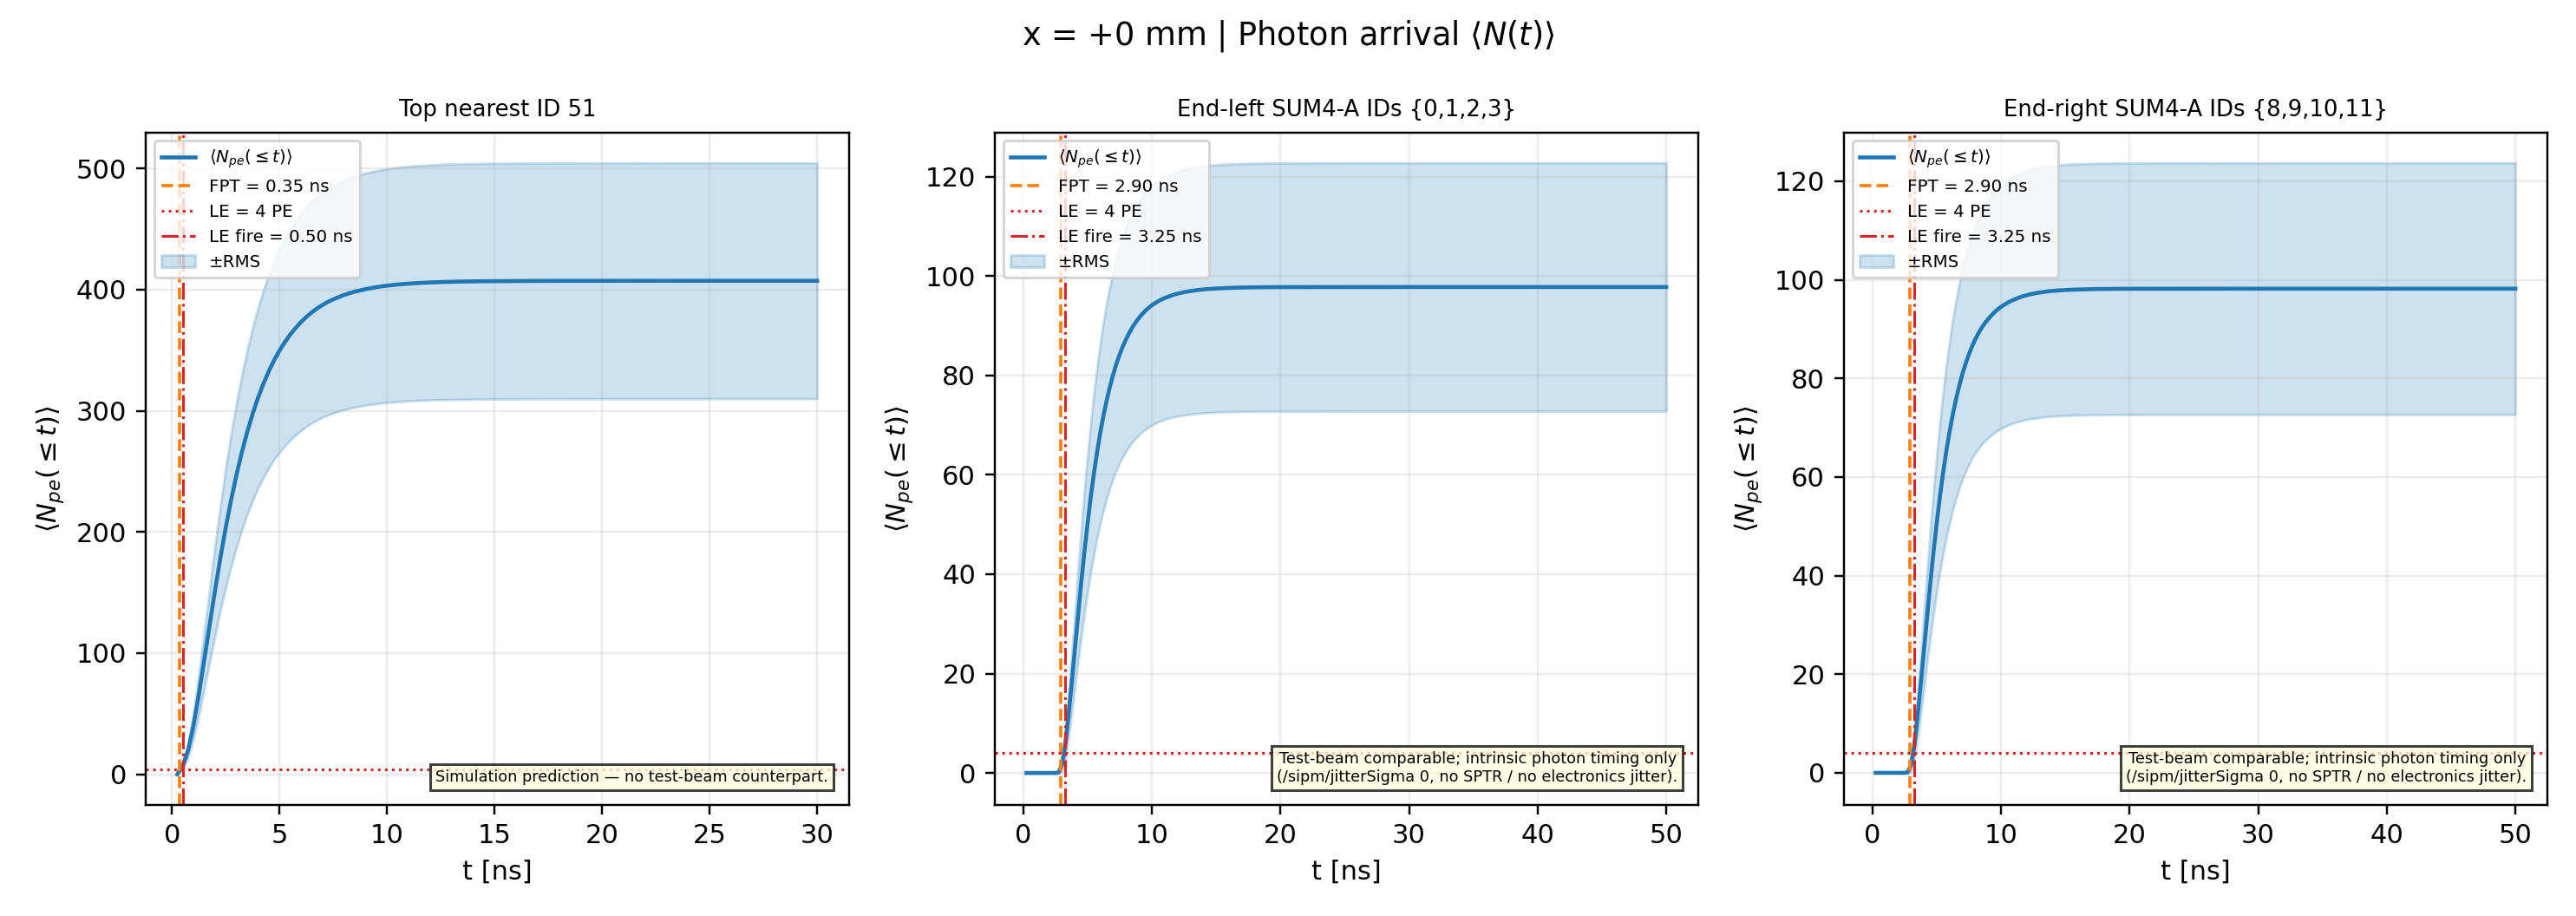
\includegraphics[width=\textwidth,height=0.78\textheight,keepaspectratio]{figs/exec11_arrival_0mm.png}
\end{frame}
\begin{frame}{Position x=50 mm}

\begin{columns}[T]
  \column{0.52\textwidth}
  
\includegraphics[width=\textwidth]{figs/muon_50mm_geometry.png}
  \column{0.46\textwidth}
  
\includegraphics[width=\textwidth]{figs/muon_50mm_top_profile.png}
  \tiny
  \begin{tabular}{lr}
    \toprule Quantity & Value \\ \midrule
    End L $N_{pe}$ & $171.6\pm1.1$ \\
    End R $N_{pe}$ & $226.4\pm1.3$ \\
    Nearest Top ID & 53 (window-track exception) \\
    Nearest Top $N_{pe}$ & $348.8\pm2.1$ \\
    Nearest Top $\langle t\rangle$ &
      $2.7787\pm0.0023$ ns \\
    Nearest Top FPT & $0.34237\pm0.00015$ ns \\
    \bottomrule
  \end{tabular}
\end{columns}

\end{frame}
\begin{frame}{Run 17 $|$ x = +50 mm $|$ Photon arrival $\langle N(t)\rangle$}
\centering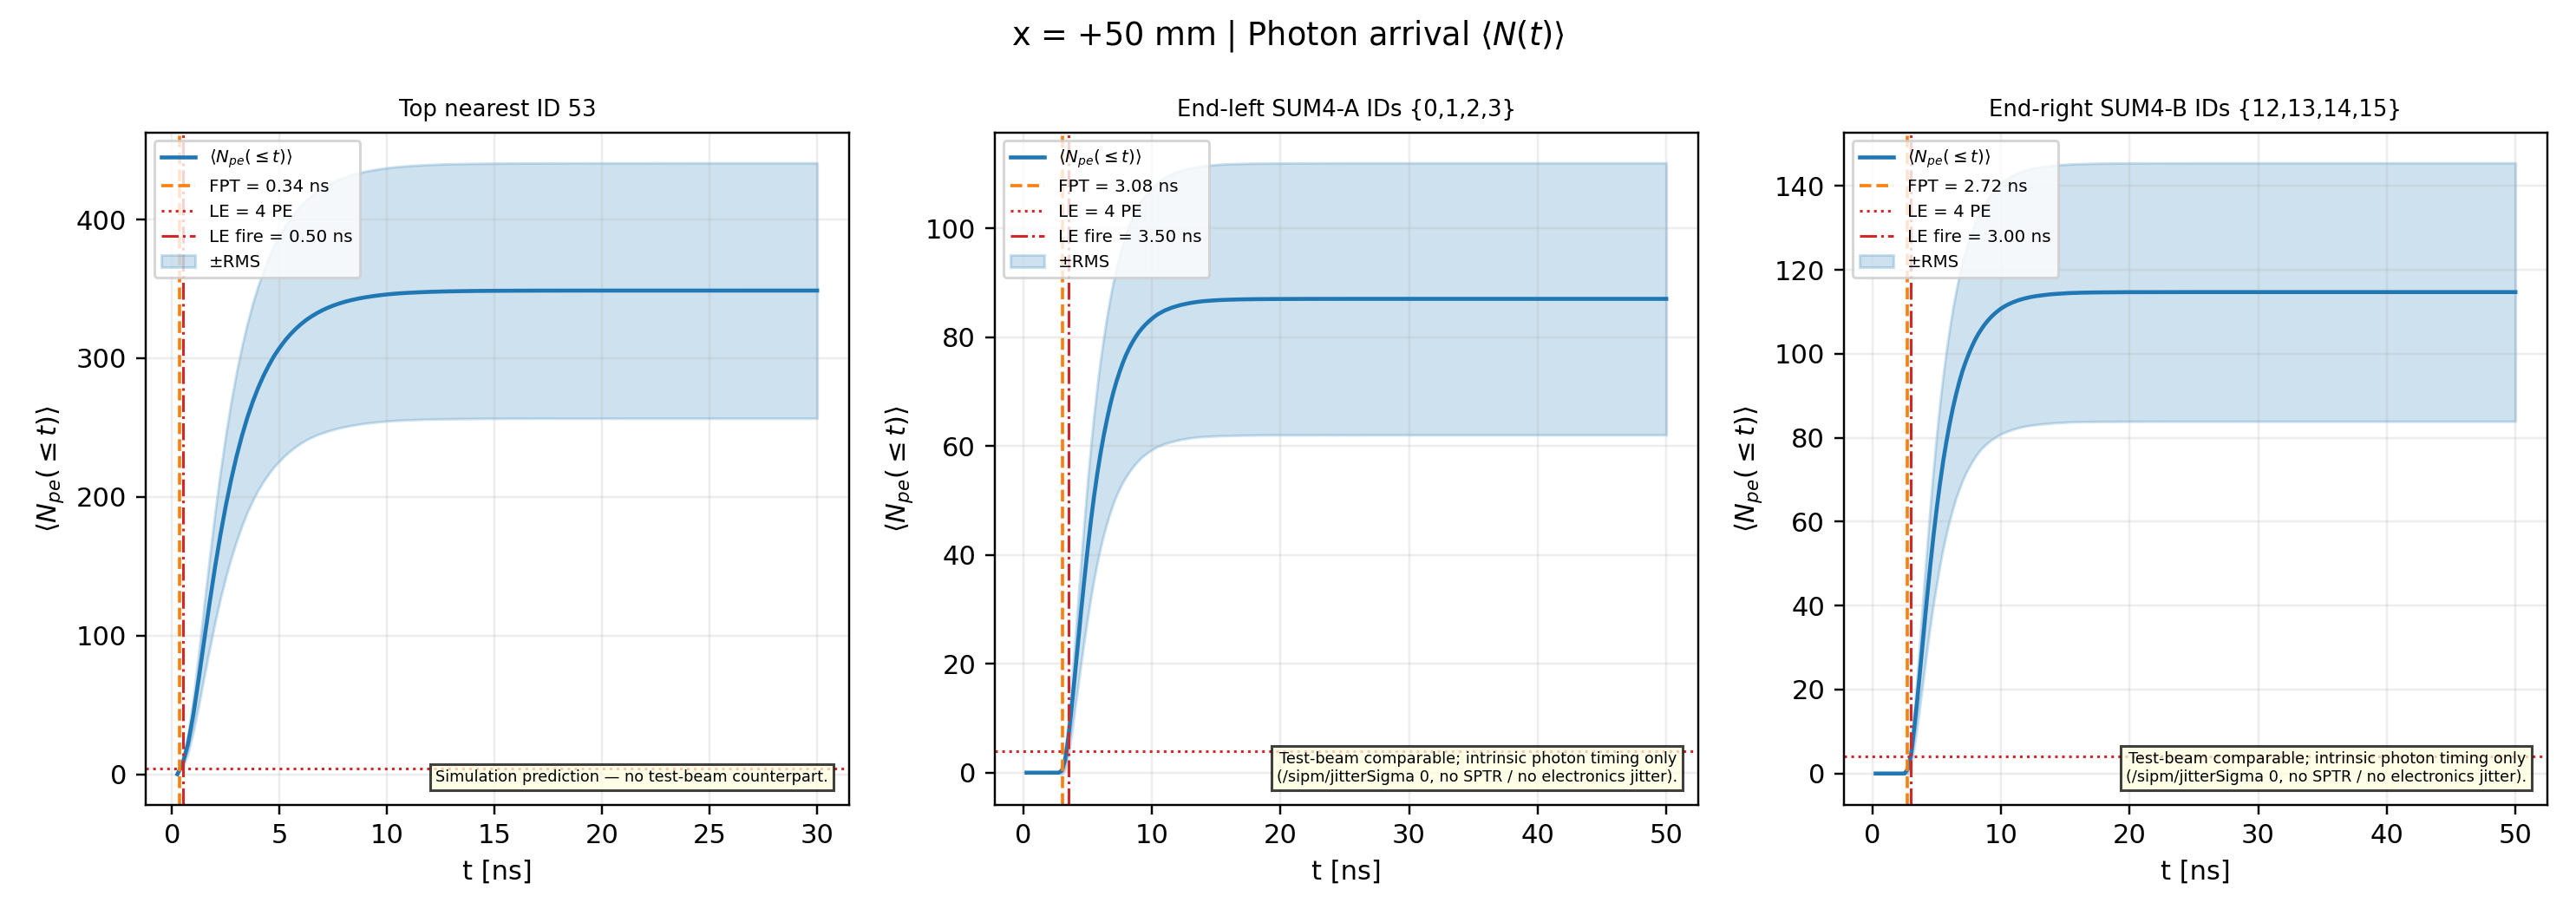
\includegraphics[width=\textwidth,height=0.78\textheight,keepaspectratio]{figs/exec11_arrival_50mm.png}
\end{frame}
\begin{frame}{Position x=100 mm}

\begin{columns}[T]
  \column{0.52\textwidth}
  
\includegraphics[width=\textwidth]{figs/muon_100mm_geometry.png}
  \column{0.46\textwidth}
  
\includegraphics[width=\textwidth]{figs/muon_100mm_top_profile.png}
  \tiny
  \begin{tabular}{lr}
    \toprule Quantity & Value \\ \midrule
    End L $N_{pe}$ & $152.2\pm0.8$ \\
    End R $N_{pe}$ & $258.3\pm1.4$ \\
    Nearest Top ID & 55 (exact geometry) \\
    Nearest Top $N_{pe}$ & $412.8\pm2.2$ \\
    Nearest Top $\langle t\rangle$ &
      $2.9429\pm0.0022$ ns \\
    Nearest Top FPT & $0.34581\pm0.00019$ ns \\
    \bottomrule
  \end{tabular}
\end{columns}

\end{frame}
\begin{frame}{Run 18 $|$ x = +100 mm $|$ Photon arrival $\langle N(t)\rangle$}
\centering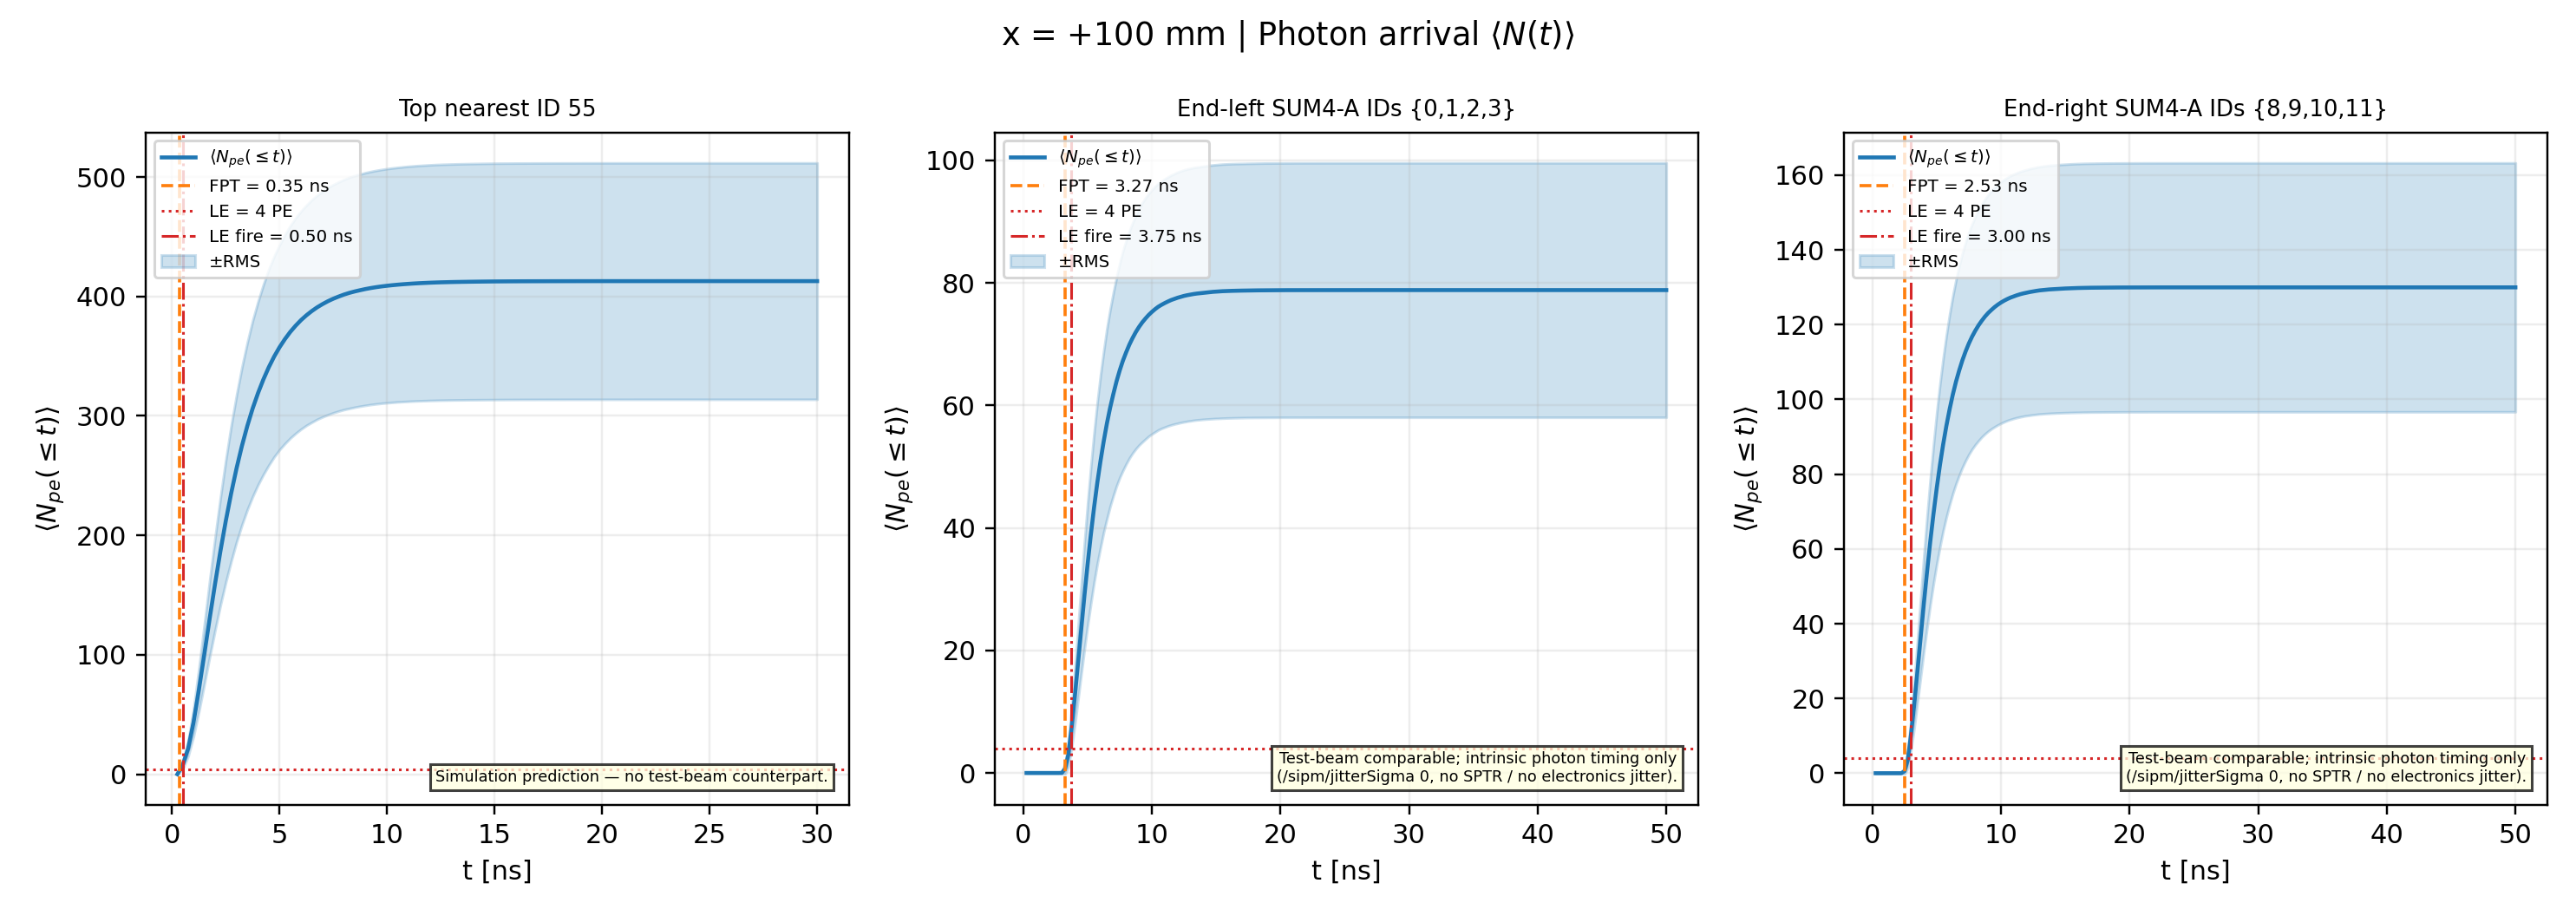
\includegraphics[width=\textwidth,height=0.78\textheight,keepaspectratio]{figs/exec11_arrival_100mm.png}
\end{frame}
\begin{frame}{Position x=150 mm}

\begin{columns}[T]
  \column{0.52\textwidth}
  
\includegraphics[width=\textwidth]{figs/muon_150mm_geometry.png}
  \column{0.46\textwidth}
  
\includegraphics[width=\textwidth]{figs/muon_150mm_top_profile.png}
  \tiny
  \begin{tabular}{lr}
    \toprule Quantity & Value \\ \midrule
    End L $N_{pe}$ & $135.5\pm0.8$ \\
    End R $N_{pe}$ & $303.6\pm1.7$ \\
    Nearest Top ID & 58 (window-track exception) \\
    Nearest Top $N_{pe}$ & $352.1\pm2.0$ \\
    Nearest Top $\langle t\rangle$ &
      $2.7821\pm0.0023$ ns \\
    Nearest Top FPT & $0.34253\pm0.00018$ ns \\
    \bottomrule
  \end{tabular}
\end{columns}

\end{frame}
\begin{frame}{Run 19 $|$ x = +150 mm $|$ Photon arrival $\langle N(t)\rangle$}
\centering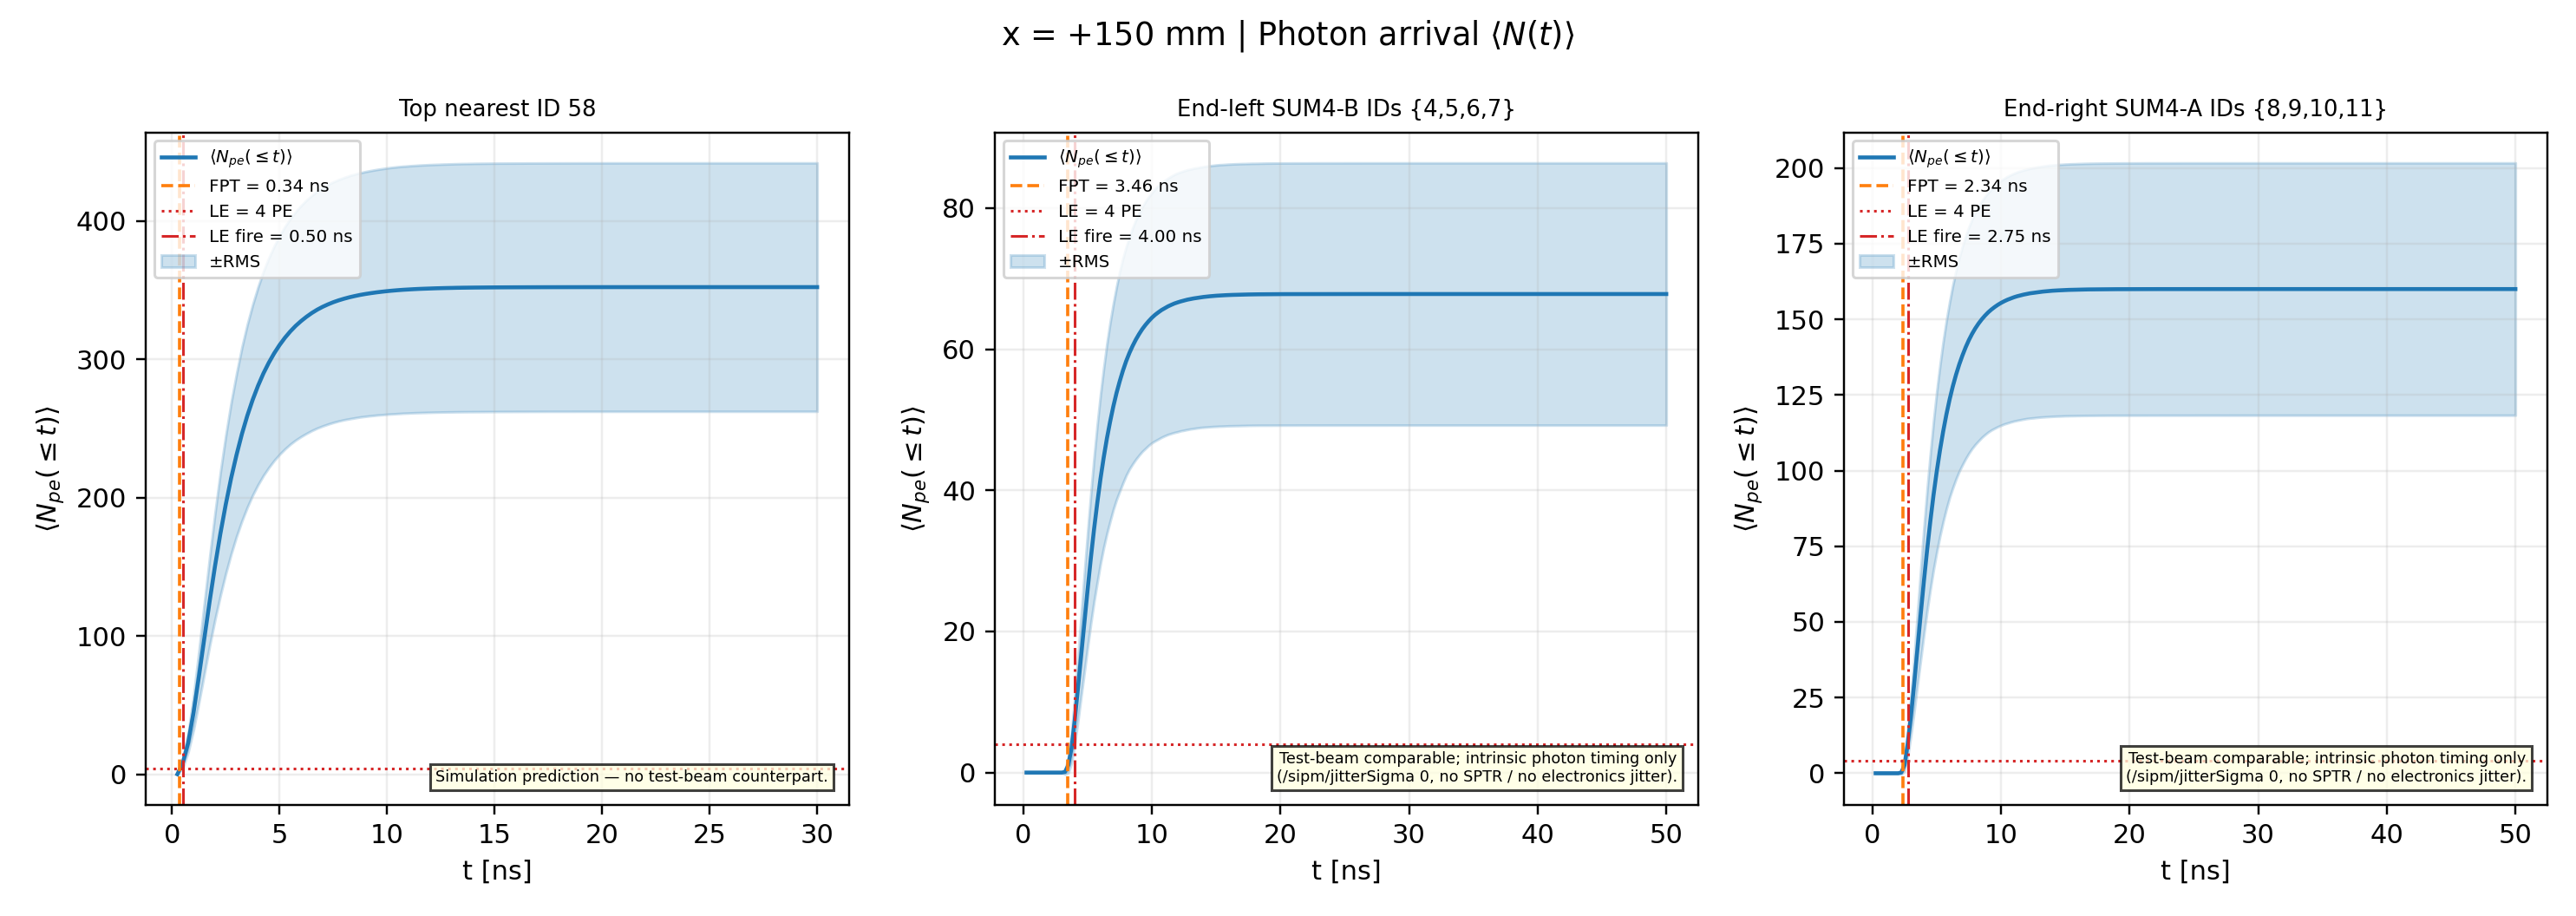
\includegraphics[width=\textwidth,height=0.78\textheight,keepaspectratio]{figs/exec11_arrival_150mm.png}
\end{frame}
\begin{frame}{Position x=200 mm}

\begin{columns}[T]
  \column{0.52\textwidth}
  
\includegraphics[width=\textwidth]{figs/muon_200mm_geometry.png}
  \column{0.46\textwidth}
  
\includegraphics[width=\textwidth]{figs/muon_200mm_top_profile.png}
  \tiny
  \begin{tabular}{lr}
    \toprule Quantity & Value \\ \midrule
    End L $N_{pe}$ & $118.5\pm0.7$ \\
    End R $N_{pe}$ & $354.1\pm2.1$ \\
    Nearest Top ID & 60 (exact geometry) \\
    Nearest Top $N_{pe}$ & $413.3\pm2.4$ \\
    Nearest Top $\langle t\rangle$ &
      $2.9367\pm0.0022$ ns \\
    Nearest Top FPT & $0.34547\pm0.00019$ ns \\
    \bottomrule
  \end{tabular}
\end{columns}

\end{frame}
\begin{frame}{Run 20 $|$ x = +200 mm $|$ Photon arrival $\langle N(t)\rangle$}
\centering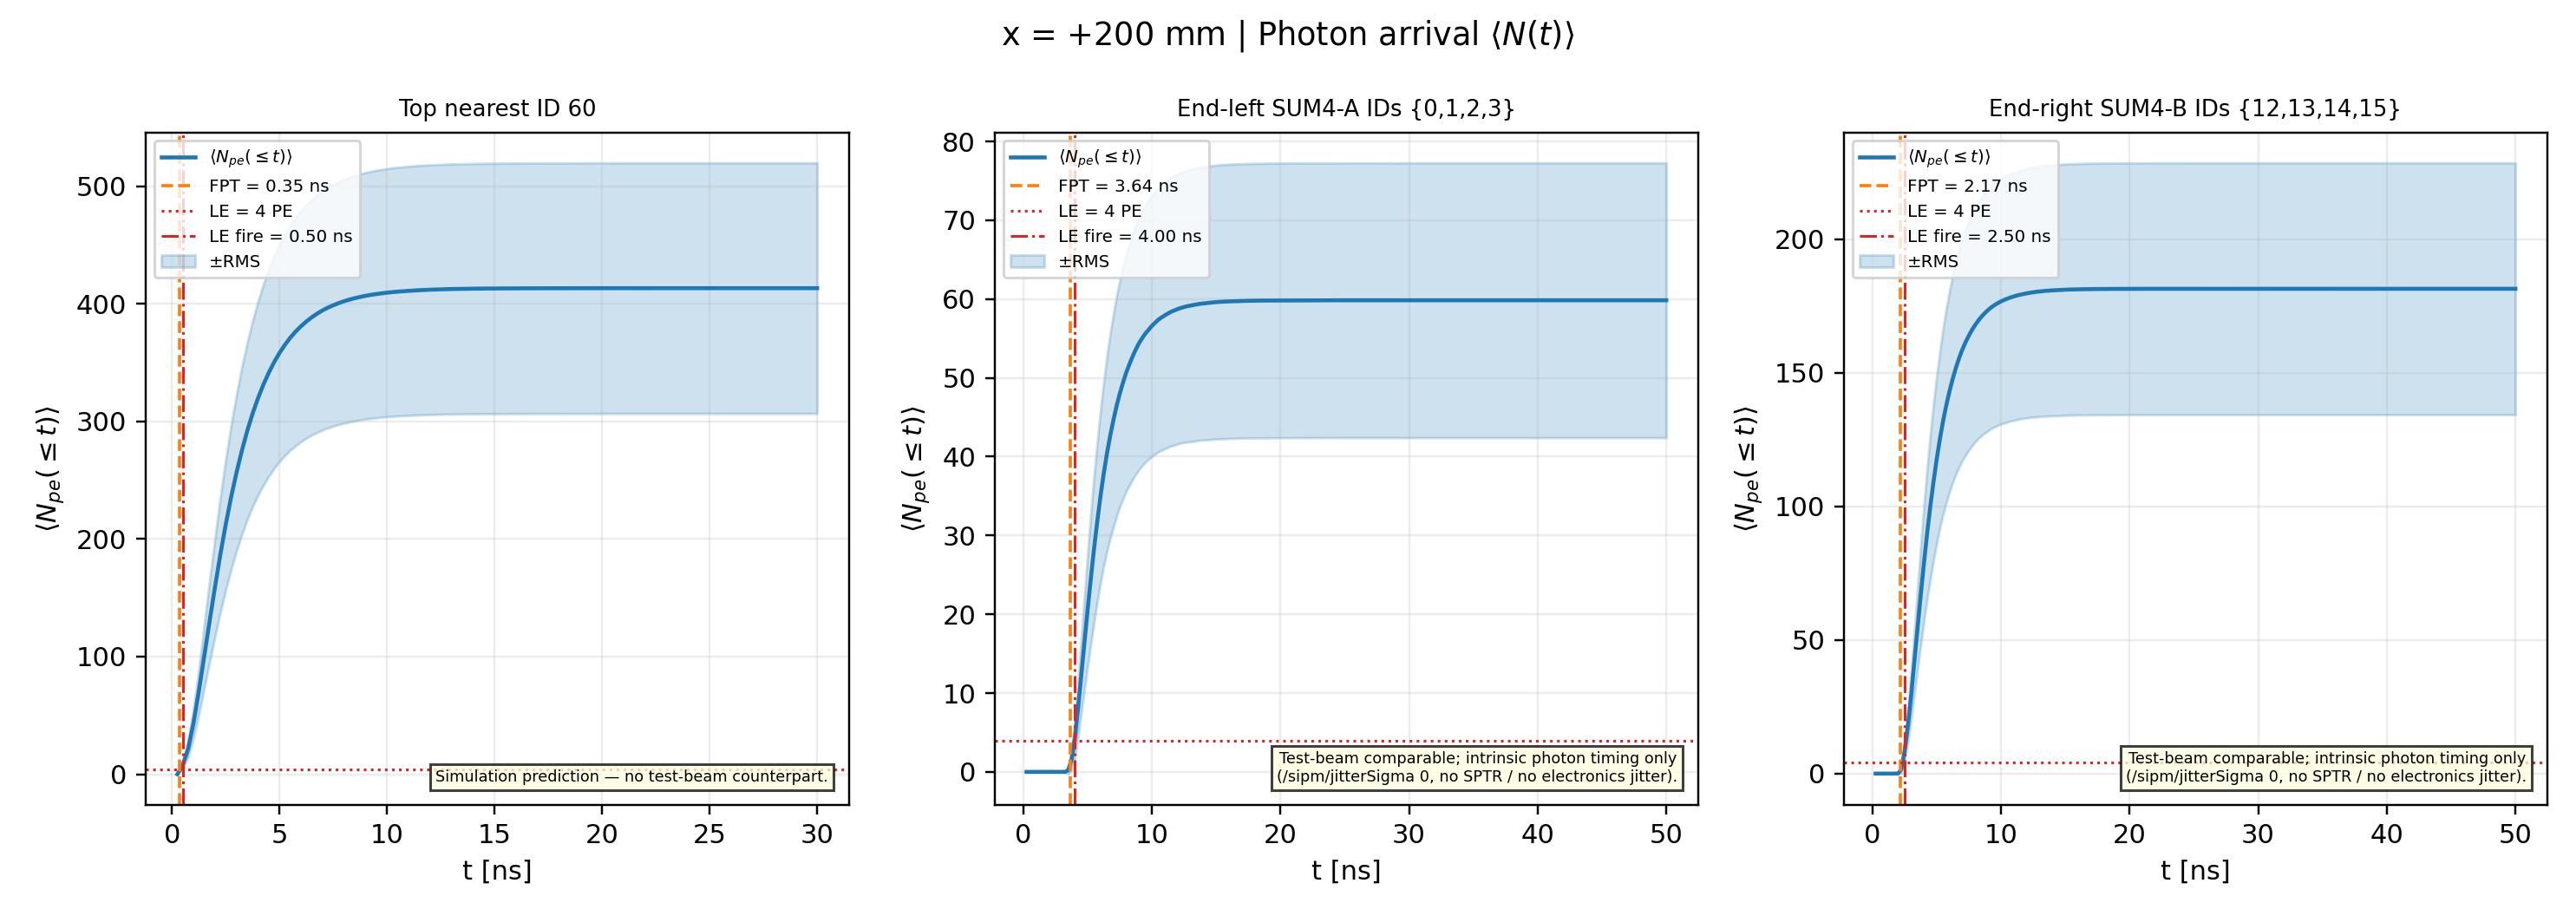
\includegraphics[width=\textwidth,height=0.78\textheight,keepaspectratio]{figs/exec11_arrival_200mm.png}
\end{frame}
\begin{frame}{Position x=250 mm}

\begin{columns}[T]
  \column{0.52\textwidth}
  
\includegraphics[width=\textwidth]{figs/muon_250mm_geometry.png}
  \column{0.46\textwidth}
  
\includegraphics[width=\textwidth]{figs/muon_250mm_top_profile.png}
  \tiny
  \begin{tabular}{lr}
    \toprule Quantity & Value \\ \midrule
    End L $N_{pe}$ & $104.8\pm0.7$ \\
    End R $N_{pe}$ & $417.0\pm2.4$ \\
    Nearest Top ID & 63 (window-track exception) \\
    Nearest Top $N_{pe}$ & $353.0\pm2.1$ \\
    Nearest Top $\langle t\rangle$ &
      $2.7759\pm0.0023$ ns \\
    Nearest Top FPT & $0.34302\pm0.00022$ ns \\
    \bottomrule
  \end{tabular}
\end{columns}

\end{frame}
\begin{frame}{Run 21 $|$ x = +250 mm $|$ Photon arrival $\langle N(t)\rangle$}
\centering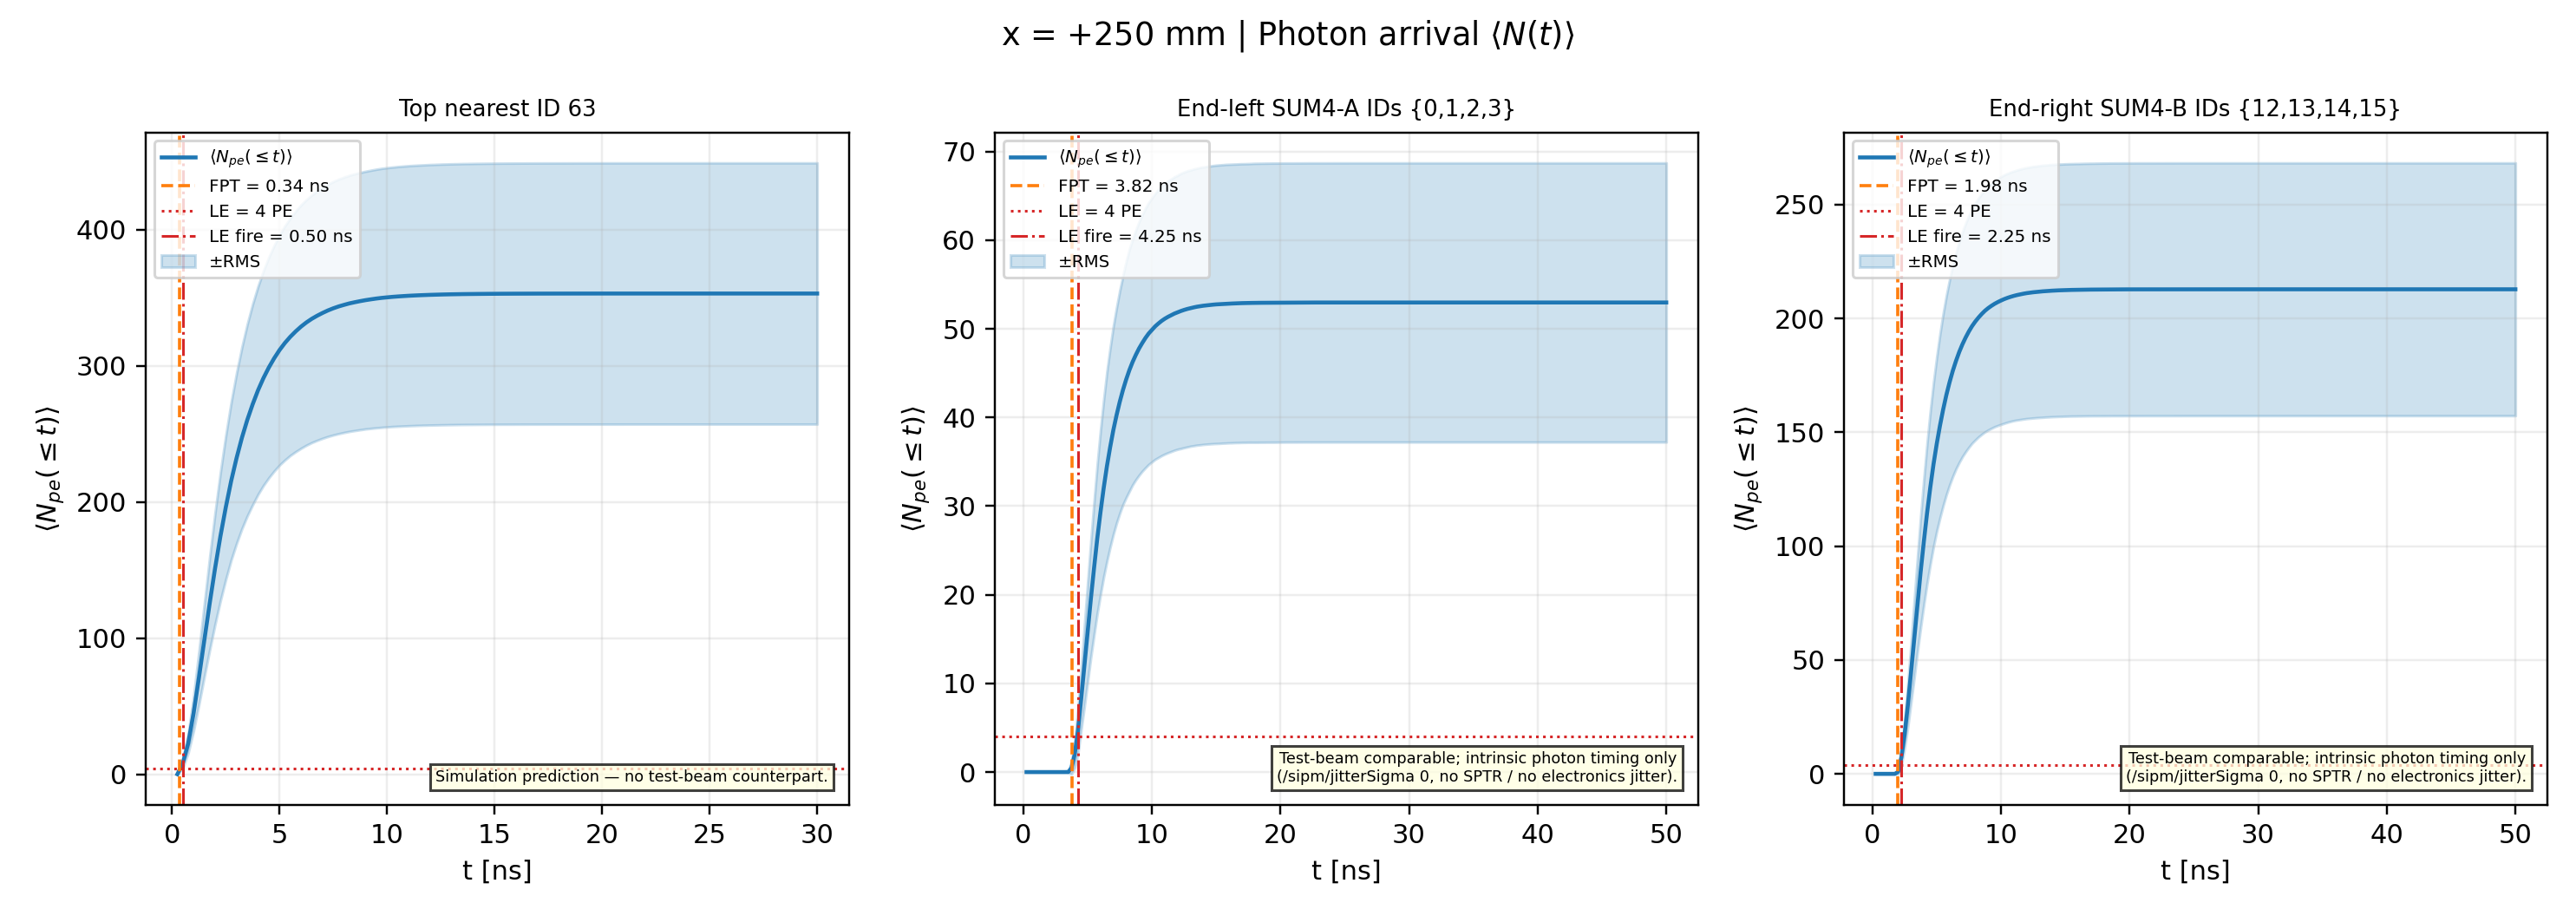
\includegraphics[width=\textwidth,height=0.78\textheight,keepaspectratio]{figs/exec11_arrival_250mm.png}
\end{frame}
\begin{frame}{Position x=300 mm}

\begin{columns}[T]
  \column{0.52\textwidth}
  
\includegraphics[width=\textwidth]{figs/muon_300mm_geometry.png}
  \column{0.46\textwidth}
  
\includegraphics[width=\textwidth]{figs/muon_300mm_top_profile.png}
  \tiny
  \begin{tabular}{lr}
    \toprule Quantity & Value \\ \midrule
    End L $N_{pe}$ & $92.5\pm0.6$ \\
    End R $N_{pe}$ & $477.5\pm2.8$ \\
    Nearest Top ID & 65 (statistical tie: two nearest) \\
    Nearest Top $N_{pe}$ & $408.7\pm2.3$ \\
    Nearest Top $\langle t\rangle$ &
      $2.9359\pm0.0022$ ns \\
    Nearest Top FPT & $0.34570\pm0.00017$ ns \\
    \bottomrule
  \end{tabular}
\end{columns}

\end{frame}
\begin{frame}{Run 22 $|$ x = +300 mm $|$ Photon arrival $\langle N(t)\rangle$}
\centering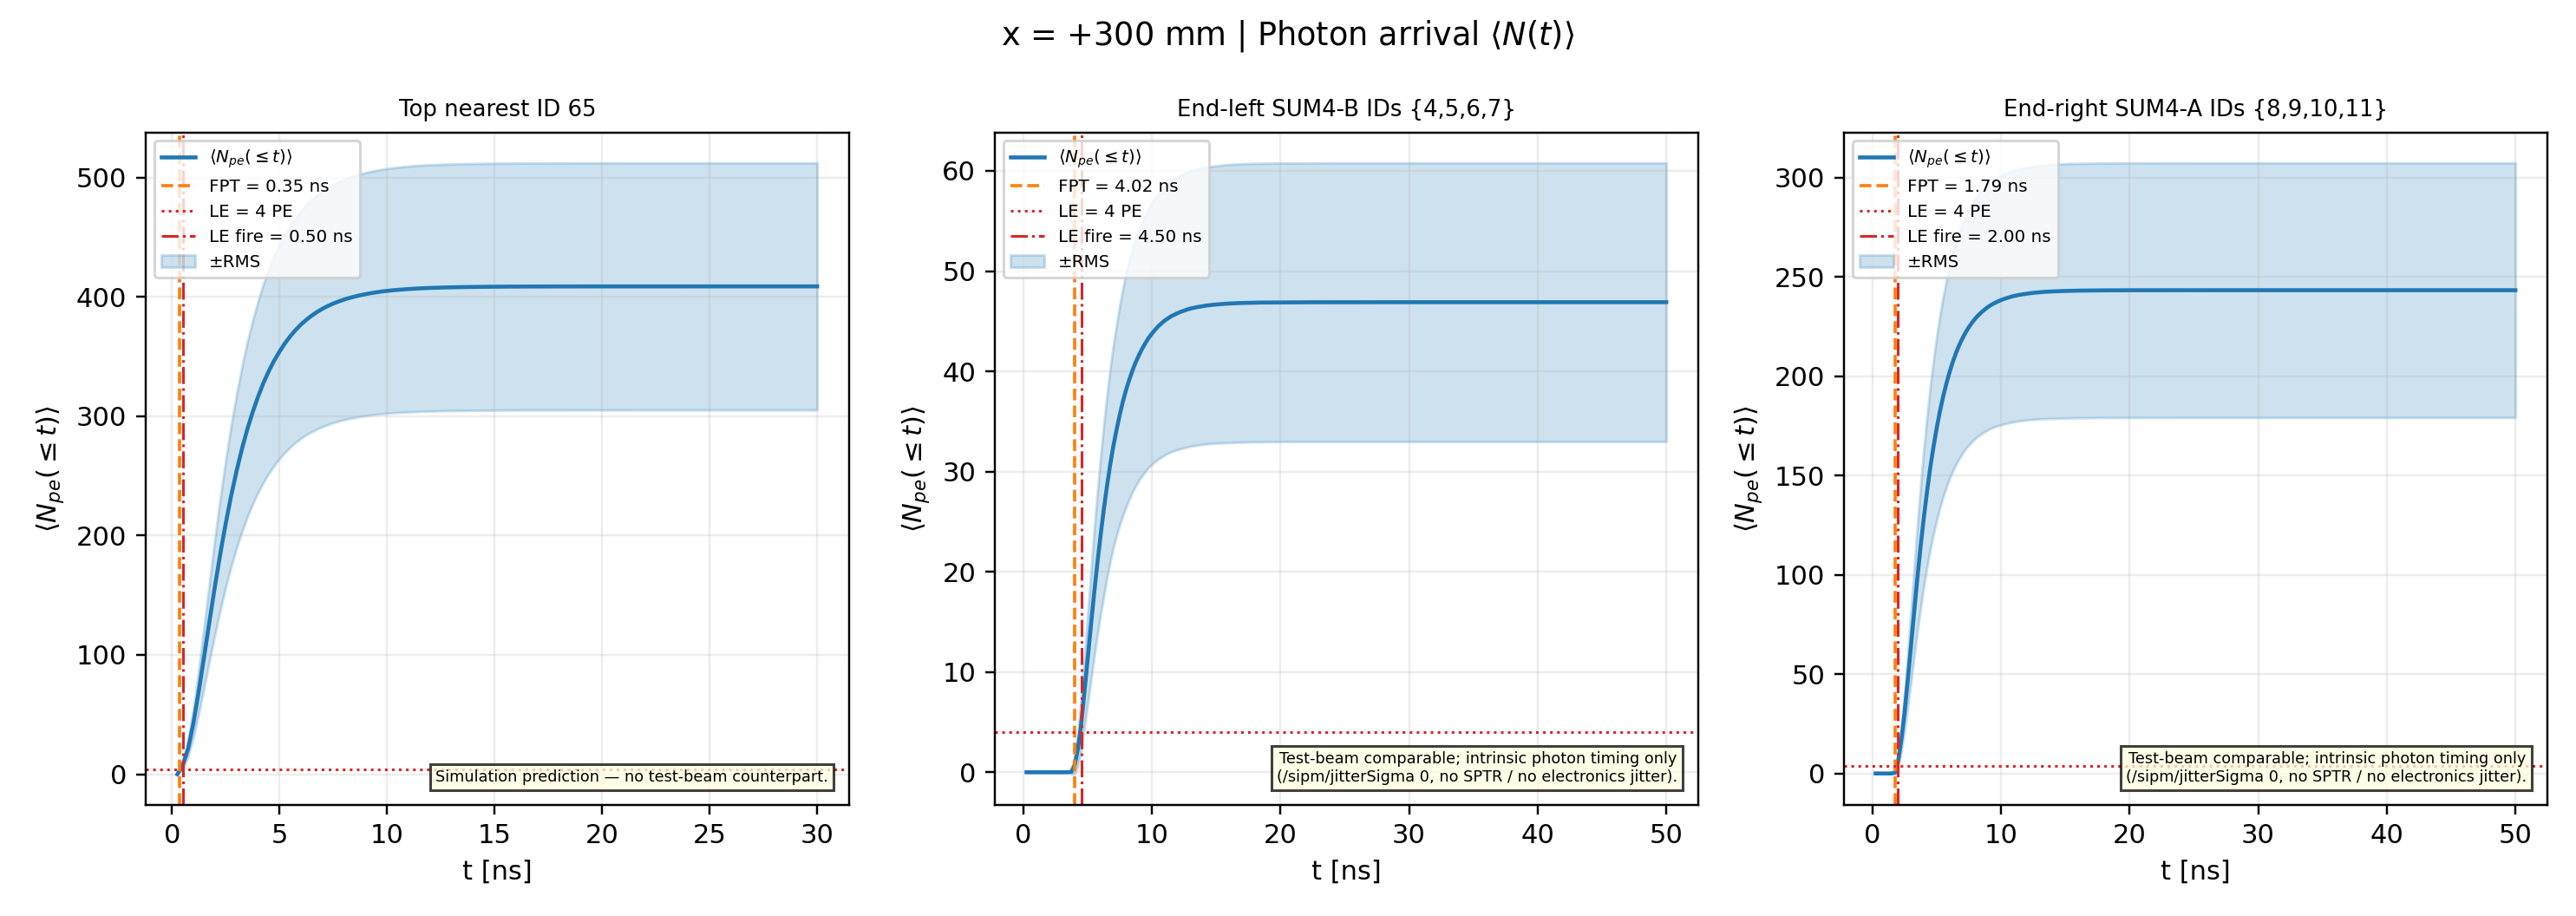
\includegraphics[width=\textwidth,height=0.78\textheight,keepaspectratio]{figs/exec11_arrival_300mm.png}
\end{frame}
\begin{frame}{Position x=350 mm}

\begin{columns}[T]
  \column{0.52\textwidth}
  
\includegraphics[width=\textwidth]{figs/muon_350mm_geometry.png}
  \column{0.46\textwidth}
  
\includegraphics[width=\textwidth]{figs/muon_350mm_top_profile.png}
  \tiny
  \begin{tabular}{lr}
    \toprule Quantity & Value \\ \midrule
    End L $N_{pe}$ & $84.0\pm0.5$ \\
    End R $N_{pe}$ & $575.5\pm3.3$ \\
    Nearest Top ID & 68 (window-track exception) \\
    Nearest Top $N_{pe}$ & $349.8\pm2.0$ \\
    Nearest Top $\langle t\rangle$ &
      $2.7768\pm0.0023$ ns \\
    Nearest Top FPT & $0.34257\pm0.00018$ ns \\
    \bottomrule
  \end{tabular}
\end{columns}

\end{frame}
\begin{frame}{Run 23 $|$ x = +350 mm $|$ Photon arrival $\langle N(t)\rangle$}
\centering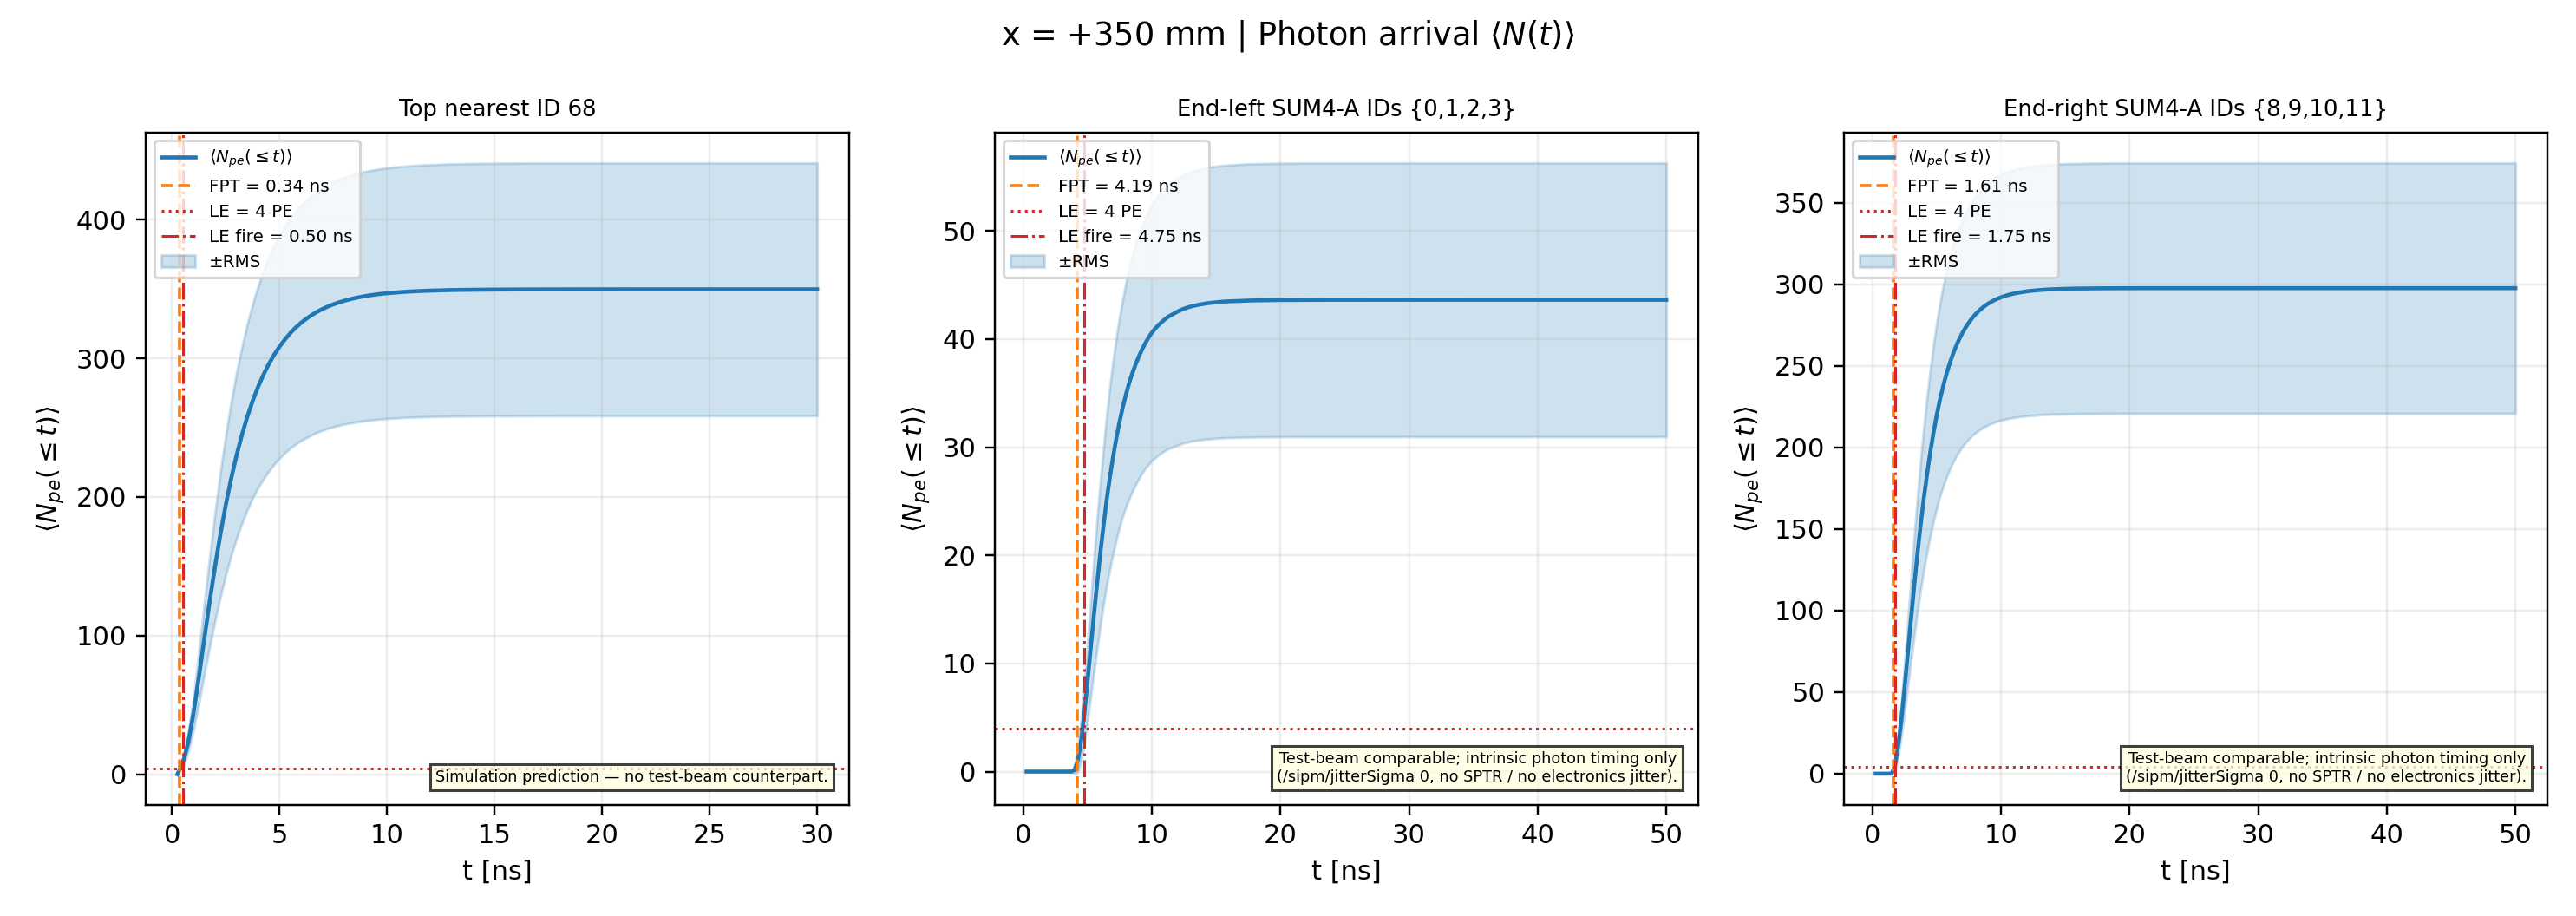
\includegraphics[width=\textwidth,height=0.78\textheight,keepaspectratio]{figs/exec11_arrival_350mm.png}
\end{frame}
\begin{frame}{Position x=400 mm}

\begin{columns}[T]
  \column{0.52\textwidth}
  
\includegraphics[width=\textwidth]{figs/muon_400mm_geometry.png}
  \column{0.46\textwidth}
  
\includegraphics[width=\textwidth]{figs/muon_400mm_top_profile.png}
  \tiny
  \begin{tabular}{lr}
    \toprule Quantity & Value \\ \midrule
    End L $N_{pe}$ & $75.0\pm0.5$ \\
    End R $N_{pe}$ & $692.5\pm4.0$ \\
    Nearest Top ID & 70 (exact geometry) \\
    Nearest Top $N_{pe}$ & $411.4\pm2.4$ \\
    Nearest Top $\langle t\rangle$ &
      $2.9433\pm0.0022$ ns \\
    Nearest Top FPT & $0.34598\pm0.00022$ ns \\
    \bottomrule
  \end{tabular}
\end{columns}

\end{frame}
\begin{frame}{Run 24 $|$ x = +400 mm $|$ Photon arrival $\langle N(t)\rangle$}
\centering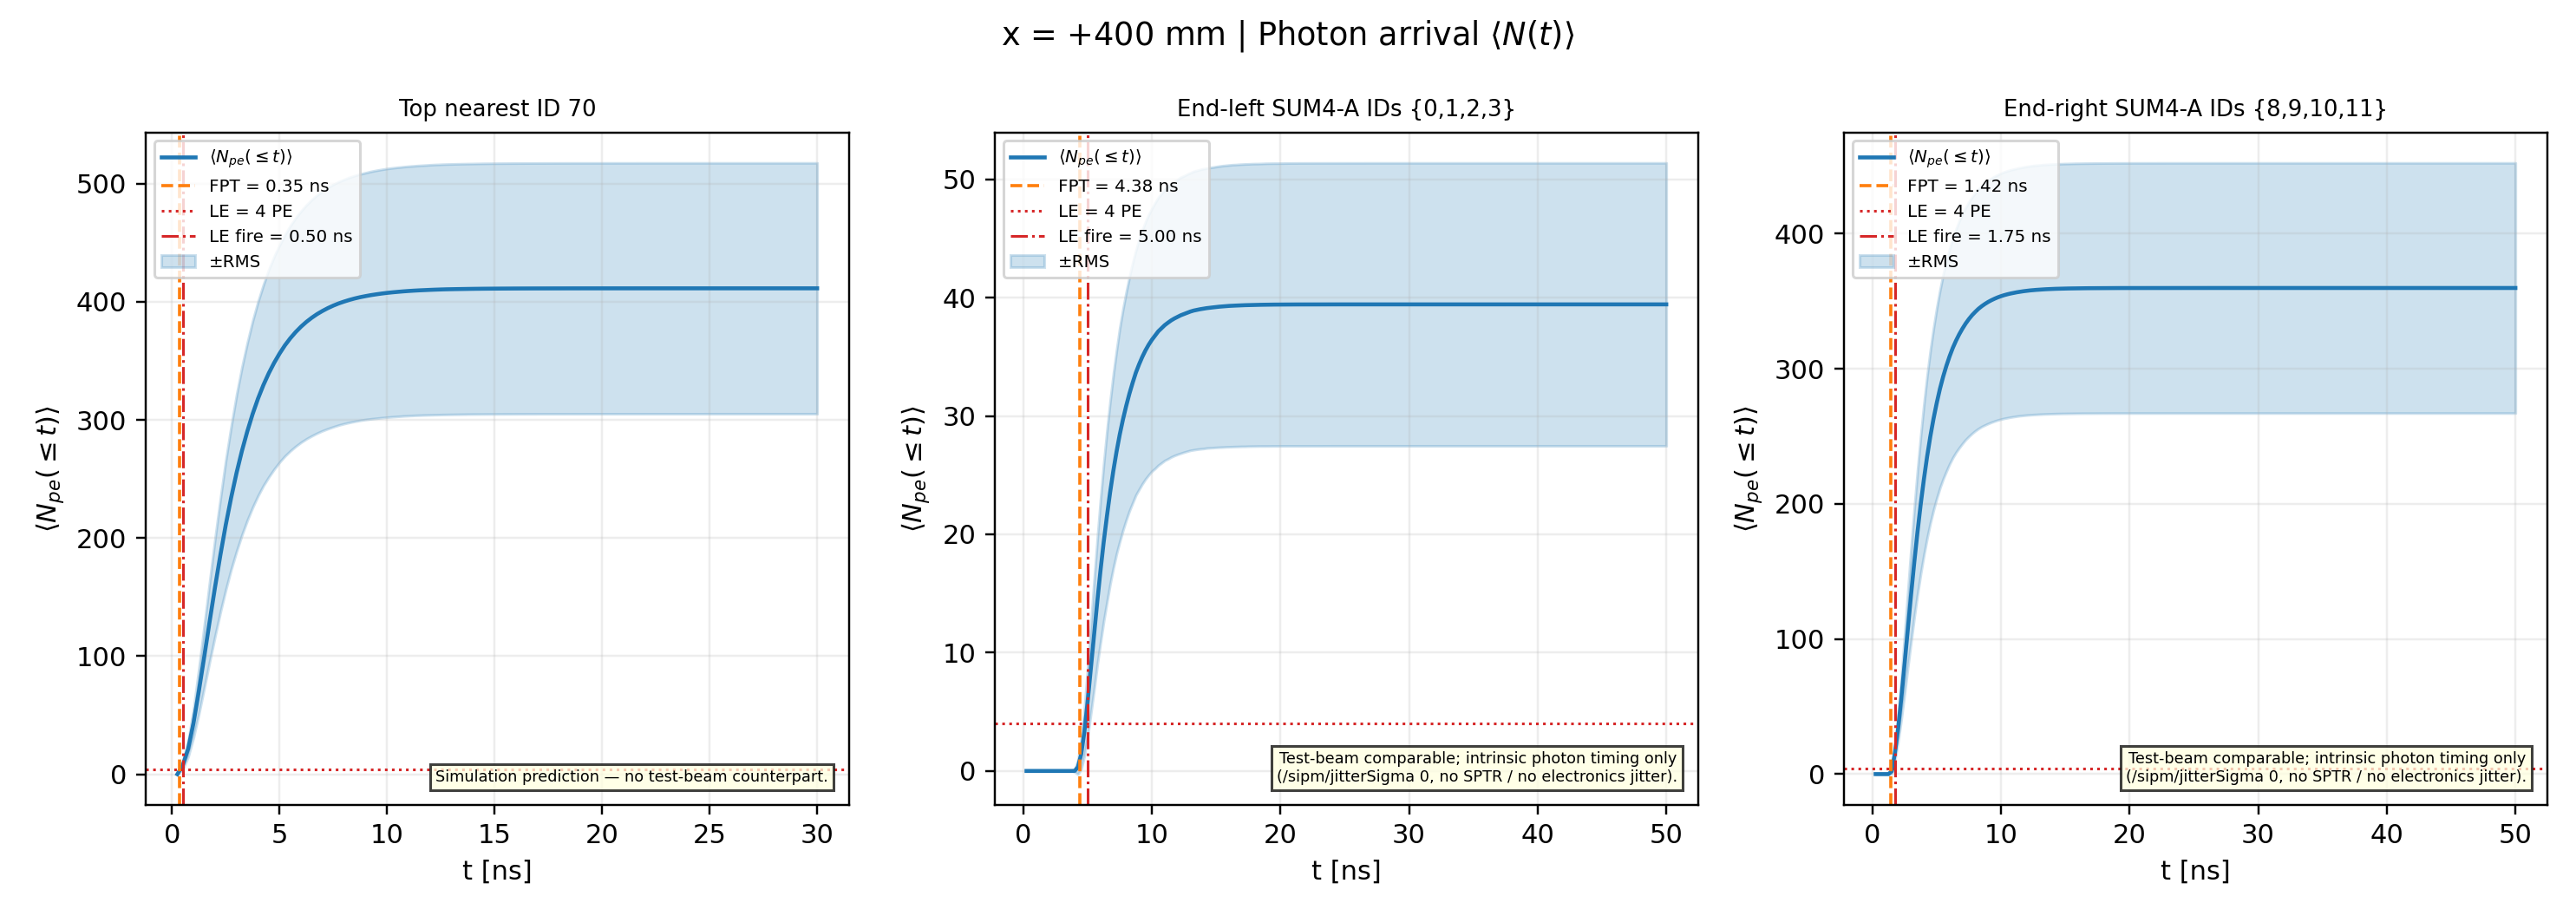
\includegraphics[width=\textwidth,height=0.78\textheight,keepaspectratio]{figs/exec11_arrival_400mm.png}
\end{frame}
\begin{frame}{Position x=450 mm}

\begin{columns}[T]
  \column{0.52\textwidth}
  
\includegraphics[width=\textwidth]{figs/muon_450mm_geometry.png}
  \column{0.46\textwidth}
  
\includegraphics[width=\textwidth]{figs/muon_450mm_top_profile.png}
  \tiny
  \begin{tabular}{lr}
    \toprule Quantity & Value \\ \midrule
    End L $N_{pe}$ & $67.1\pm0.4$ \\
    End R $N_{pe}$ & $845.1\pm4.8$ \\
    Nearest Top ID & 73 (window-track exception) \\
    Nearest Top $N_{pe}$ & $352.2\pm2.1$ \\
    Nearest Top $\langle t\rangle$ &
      $2.7735\pm0.0023$ ns \\
    Nearest Top FPT & $0.34289\pm0.00024$ ns \\
    \bottomrule
  \end{tabular}
\end{columns}

\end{frame}
\begin{frame}{Run 25 $|$ x = +450 mm $|$ Photon arrival $\langle N(t)\rangle$}
\centering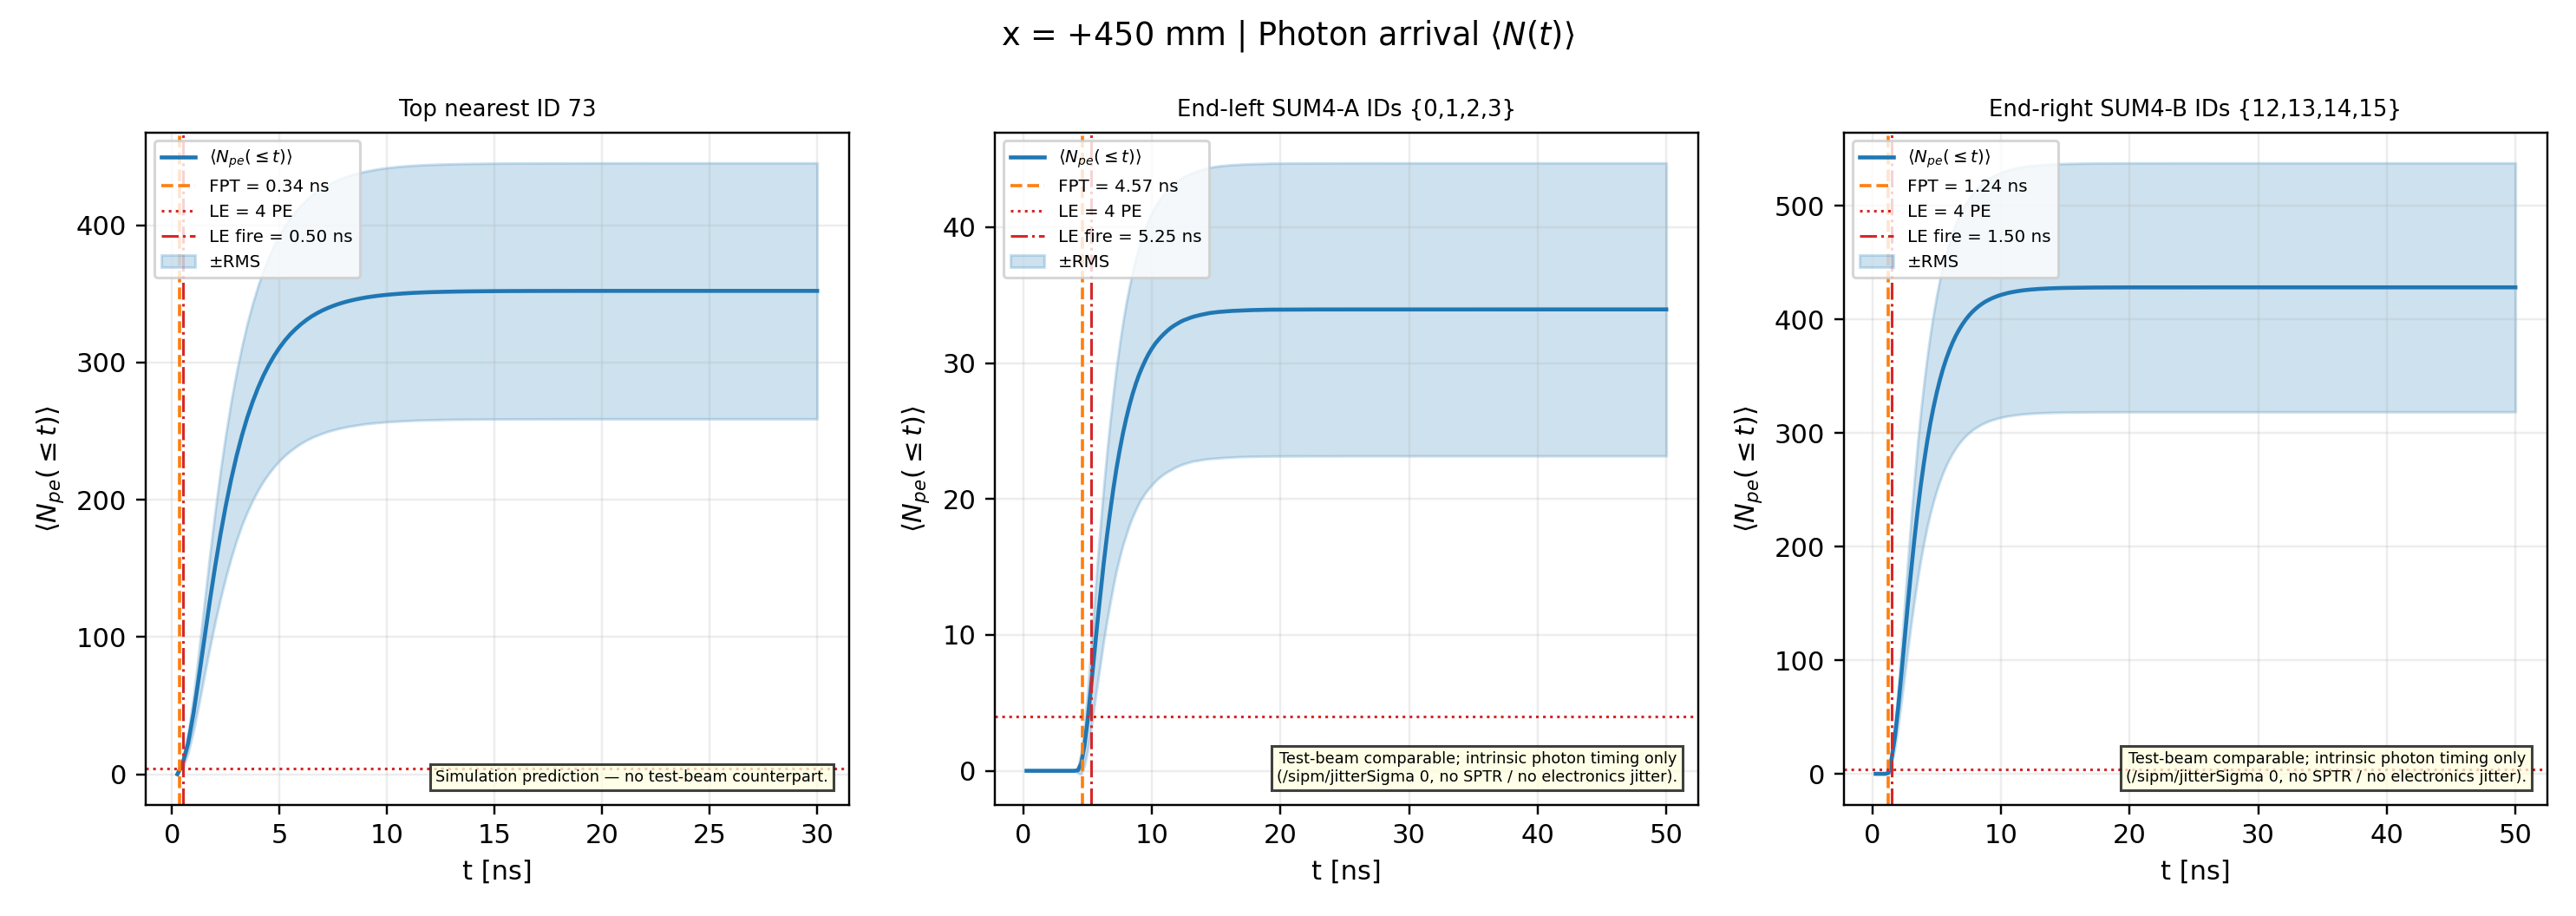
\includegraphics[width=\textwidth,height=0.78\textheight,keepaspectratio]{figs/exec11_arrival_450mm.png}
\end{frame}
\begin{frame}{Position x=500 mm}

\begin{columns}[T]
  \column{0.52\textwidth}
  
\includegraphics[width=\textwidth]{figs/muon_500mm_geometry.png}
  \column{0.46\textwidth}
  
\includegraphics[width=\textwidth]{figs/muon_500mm_top_profile.png}
  \tiny
  \begin{tabular}{lr}
    \toprule Quantity & Value \\ \midrule
    End L $N_{pe}$ & $59.9\pm0.4$ \\
    End R $N_{pe}$ & $1039.9\pm5.9$ \\
    Nearest Top ID & 75 (exact geometry) \\
    Nearest Top $N_{pe}$ & $410.5\pm2.3$ \\
    Nearest Top $\langle t\rangle$ &
      $2.9405\pm0.0022$ ns \\
    Nearest Top FPT & $0.34627\pm0.00026$ ns \\
    \bottomrule
  \end{tabular}
\end{columns}

\end{frame}
\begin{frame}{Run 26 $|$ x = +500 mm $|$ Photon arrival $\langle N(t)\rangle$}
\centering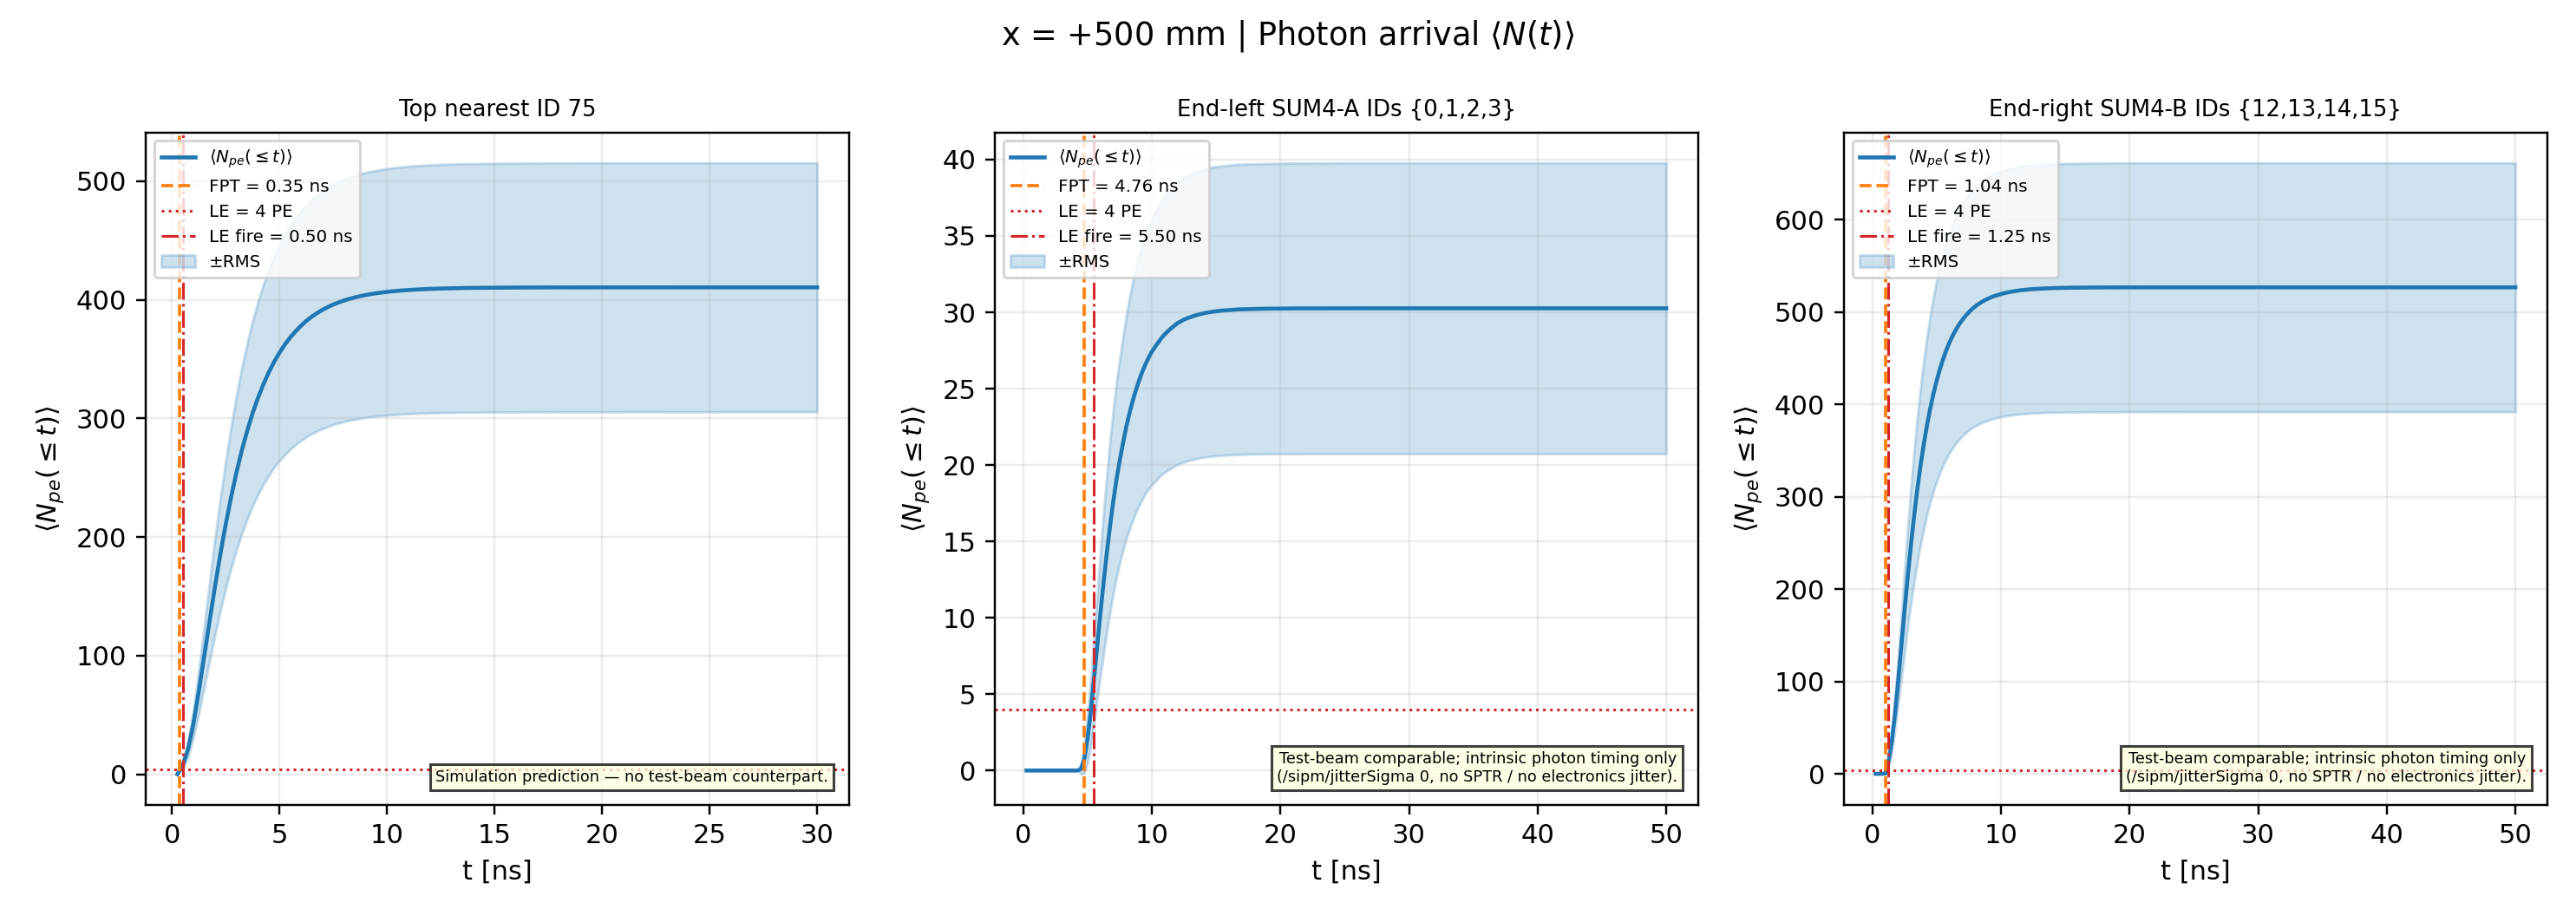
\includegraphics[width=\textwidth,height=0.78\textheight,keepaspectratio]{figs/exec11_arrival_500mm.png}
\end{frame}
\begin{frame}{Position x=550 mm}

\begin{columns}[T]
  \column{0.52\textwidth}
  
\includegraphics[width=\textwidth]{figs/muon_550mm_geometry.png}
  \column{0.46\textwidth}
  
\includegraphics[width=\textwidth]{figs/muon_550mm_top_profile.png}
  \tiny
  \begin{tabular}{lr}
    \toprule Quantity & Value \\ \midrule
    End L $N_{pe}$ & $55.1\pm0.4$ \\
    End R $N_{pe}$ & $1325.9\pm7.7$ \\
    Nearest Top ID & 78 (window-track exception) \\
    Nearest Top $N_{pe}$ & $352.3\pm2.1$ \\
    Nearest Top $\langle t\rangle$ &
      $2.7796\pm0.0023$ ns \\
    Nearest Top FPT & $0.34251\pm0.00021$ ns \\
    \bottomrule
  \end{tabular}
\end{columns}

\end{frame}
\begin{frame}{Run 27 $|$ x = +550 mm $|$ Photon arrival $\langle N(t)\rangle$}
\centering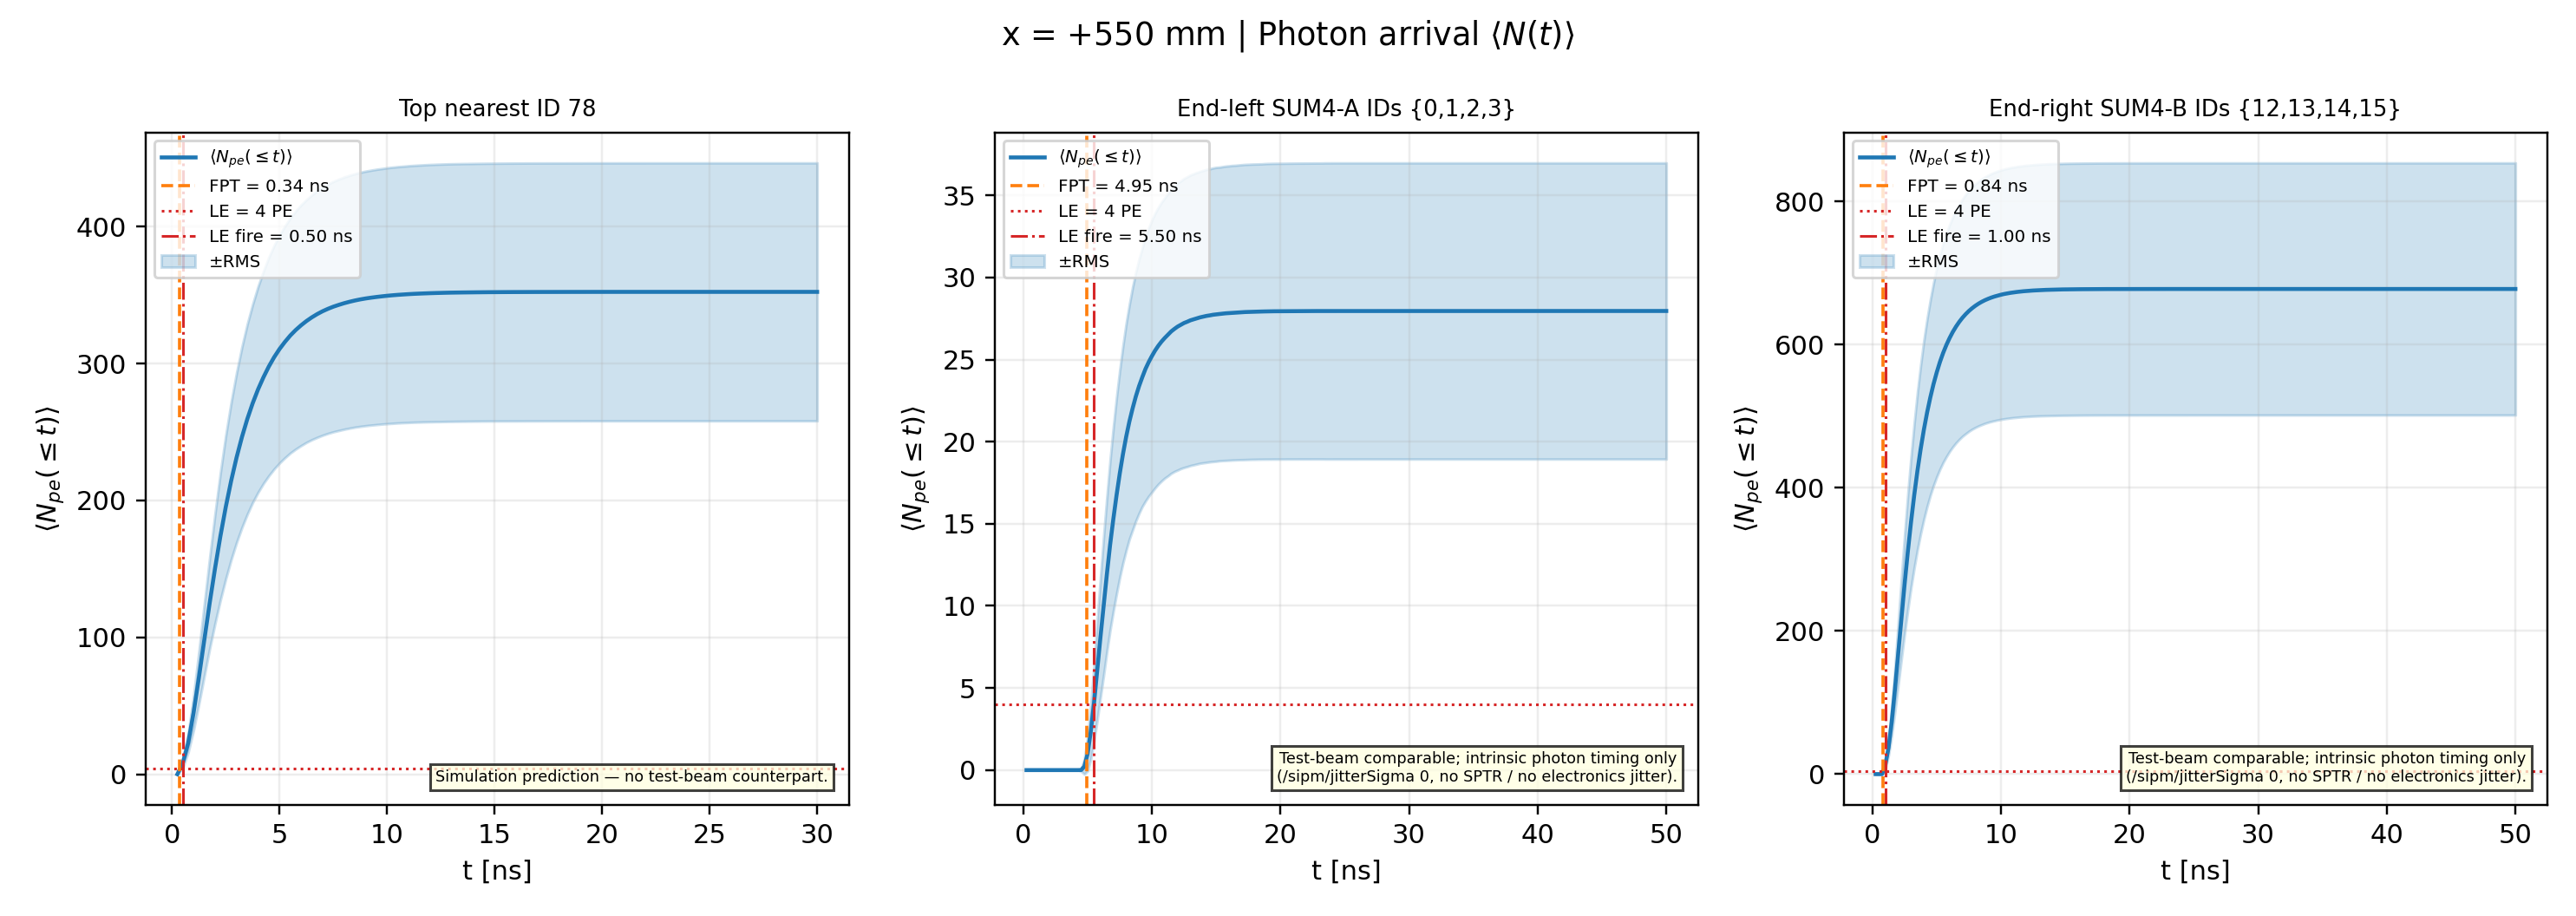
\includegraphics[width=\textwidth,height=0.78\textheight,keepaspectratio]{figs/exec11_arrival_550mm.png}
\end{frame}
\begin{frame}{Position x=600 mm}

\begin{columns}[T]
  \column{0.52\textwidth}
  
\includegraphics[width=\textwidth]{figs/muon_600mm_geometry.png}
  \column{0.46\textwidth}
  
\includegraphics[width=\textwidth]{figs/muon_600mm_top_profile.png}
  \tiny
  \begin{tabular}{lr}
    \toprule Quantity & Value \\ \midrule
    End L $N_{pe}$ & $48.6\pm0.3$ \\
    End R $N_{pe}$ & $1687.6\pm9.3$ \\
    Nearest Top ID & 80 (exact geometry) \\
    Nearest Top $N_{pe}$ & $411.6\pm2.3$ \\
    Nearest Top $\langle t\rangle$ &
      $2.9383\pm0.0022$ ns \\
    Nearest Top FPT & $0.34587\pm0.00023$ ns \\
    \bottomrule
  \end{tabular}
\end{columns}

\end{frame}
\begin{frame}{Run 28 $|$ x = +600 mm $|$ Photon arrival $\langle N(t)\rangle$}
\centering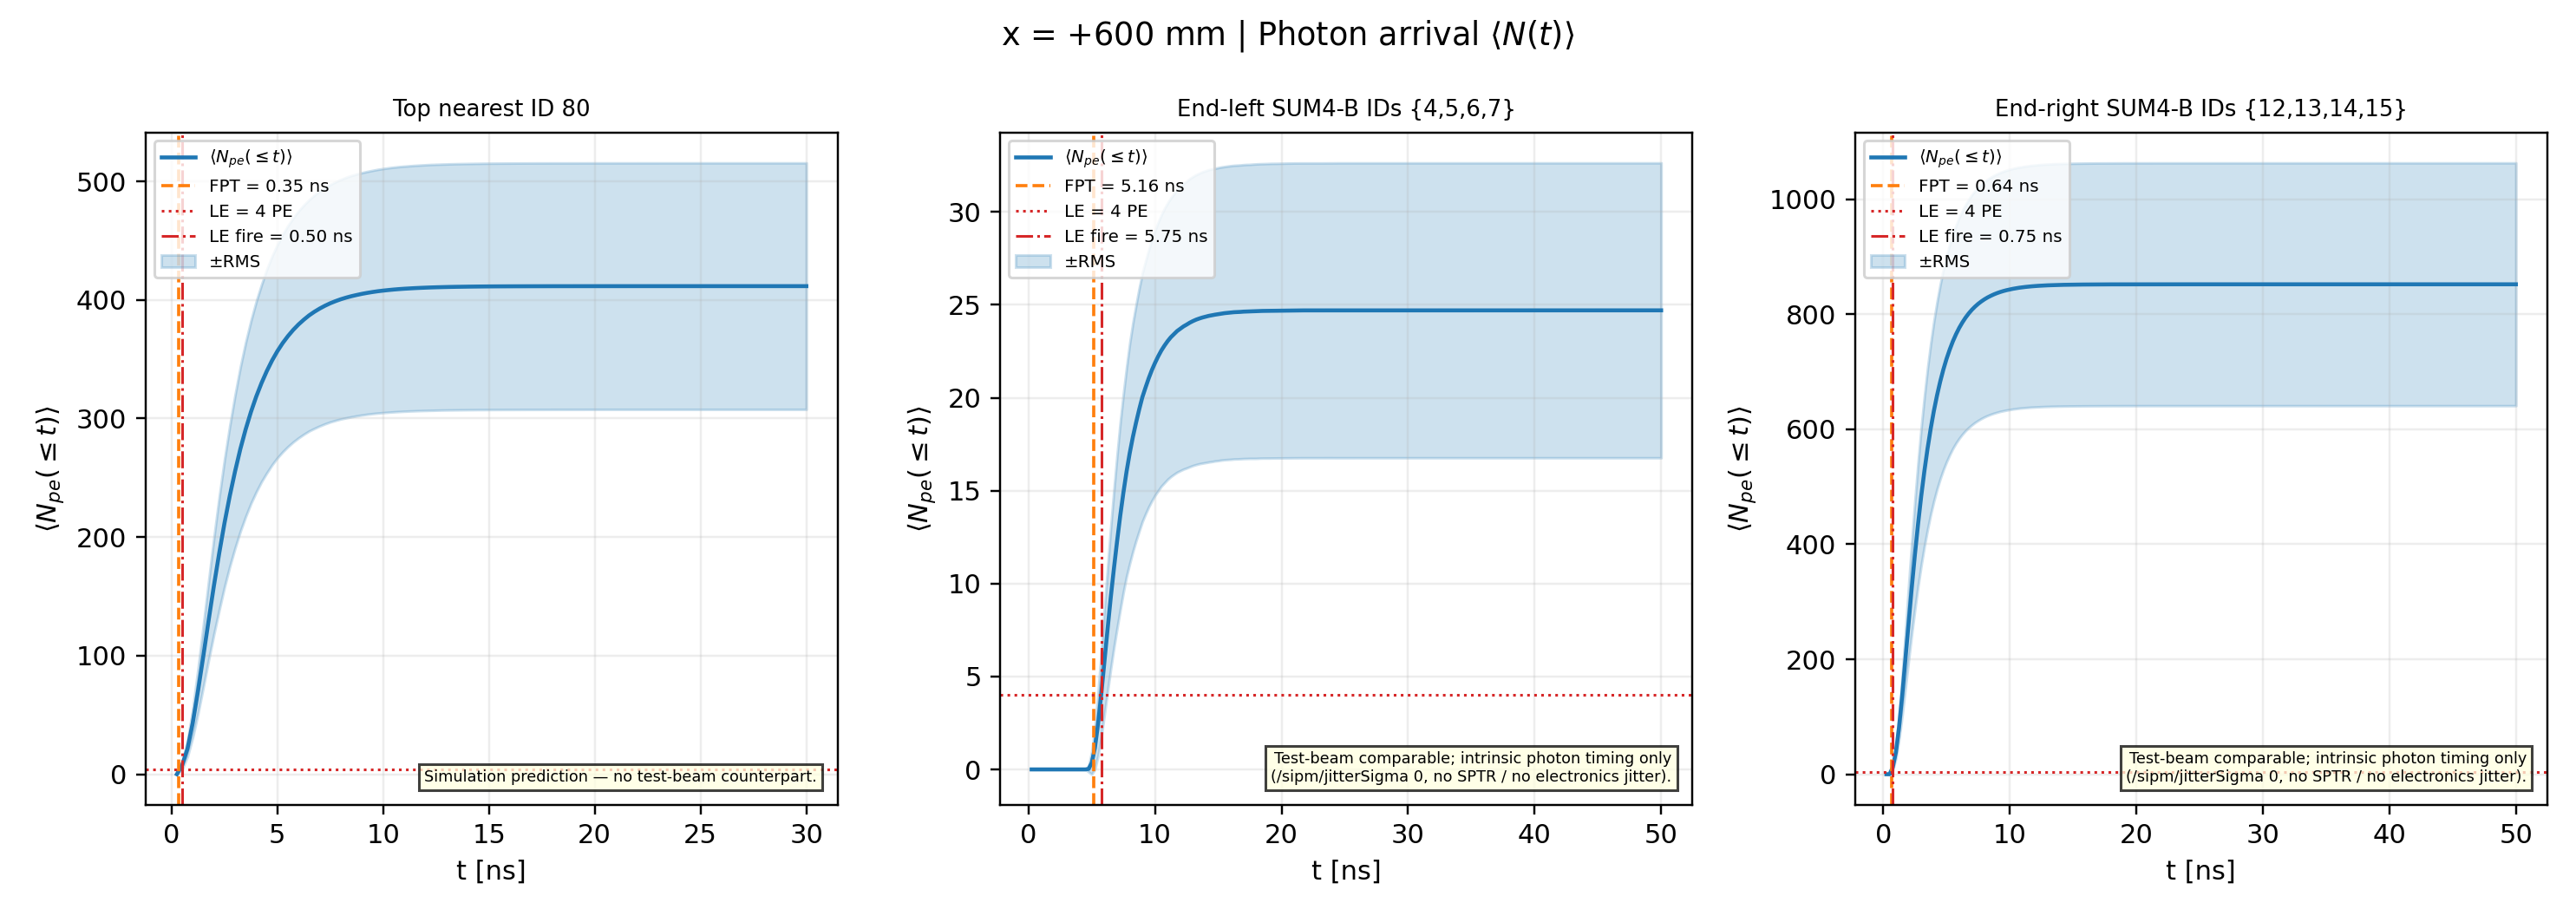
\includegraphics[width=\textwidth,height=0.78\textheight,keepaspectratio]{figs/exec11_arrival_600mm.png}
\end{frame}
\begin{frame}{Position x=650 mm}

\begin{columns}[T]
  \column{0.52\textwidth}
  
\includegraphics[width=\textwidth]{figs/muon_650mm_geometry.png}
  \column{0.46\textwidth}
  
\includegraphics[width=\textwidth]{figs/muon_650mm_top_profile.png}
  \tiny
  \begin{tabular}{lr}
    \toprule Quantity & Value \\ \midrule
    End L $N_{pe}$ & $44.4\pm0.3$ \\
    End R $N_{pe}$ & $2357.1\pm13.0$ \\
    Nearest Top ID & 83 (window-track exception) \\
    Nearest Top $N_{pe}$ & $350.9\pm2.1$ \\
    Nearest Top $\langle t\rangle$ &
      $2.7803\pm0.0023$ ns \\
    Nearest Top FPT & $0.34268\pm0.00021$ ns \\
    \bottomrule
  \end{tabular}
\end{columns}

\end{frame}
\begin{frame}{Run 29 $|$ x = +650 mm $|$ Photon arrival $\langle N(t)\rangle$}
\centering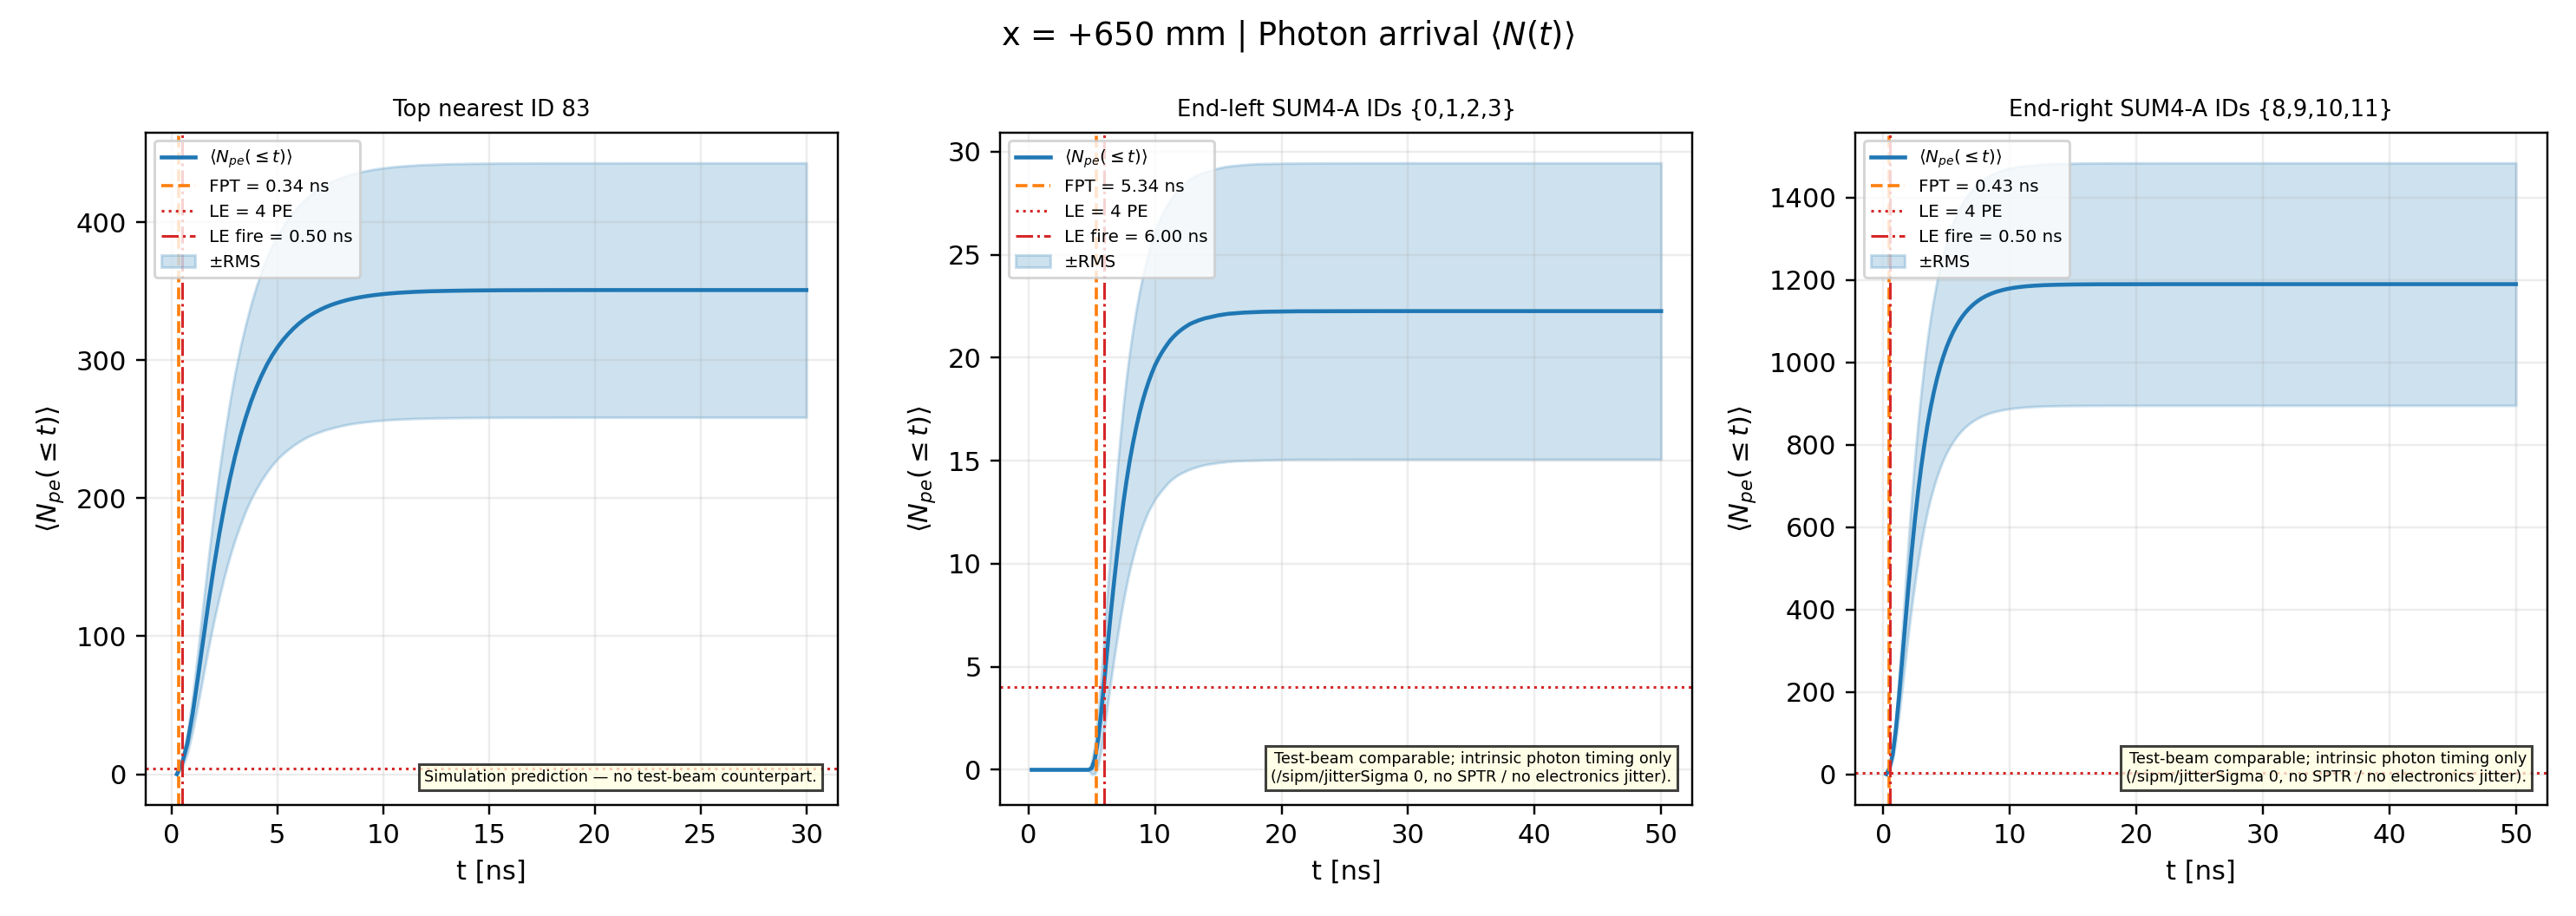
\includegraphics[width=\textwidth,height=0.78\textheight,keepaspectratio]{figs/exec11_arrival_650mm.png}
\end{frame}
\begin{frame}{Position x=670 mm}

\begin{columns}[T]
  \column{0.52\textwidth}
  
\includegraphics[width=\textwidth]{figs/muon_670mm_geometry.png}
  \column{0.46\textwidth}
  
\includegraphics[width=\textwidth]{figs/muon_670mm_top_profile.png}
  \tiny
  \begin{tabular}{lr}
    \toprule Quantity & Value \\ \midrule
    End L $N_{pe}$ & $42.2\pm0.3$ \\
    End R $N_{pe}$ & $2763.5\pm15.3$ \\
    Nearest Top ID & 84 (window-track exception) \\
    Nearest Top $N_{pe}$ & $350.2\pm2.0$ \\
    Nearest Top $\langle t\rangle$ &
      $2.7833\pm0.0023$ ns \\
    Nearest Top FPT & $0.34231\pm0.00014$ ns \\
    \bottomrule
  \end{tabular}
\end{columns}

\end{frame}
\begin{frame}{Run 30 $|$ x = +670 mm $|$ Photon arrival $\langle N(t)\rangle$}
\centering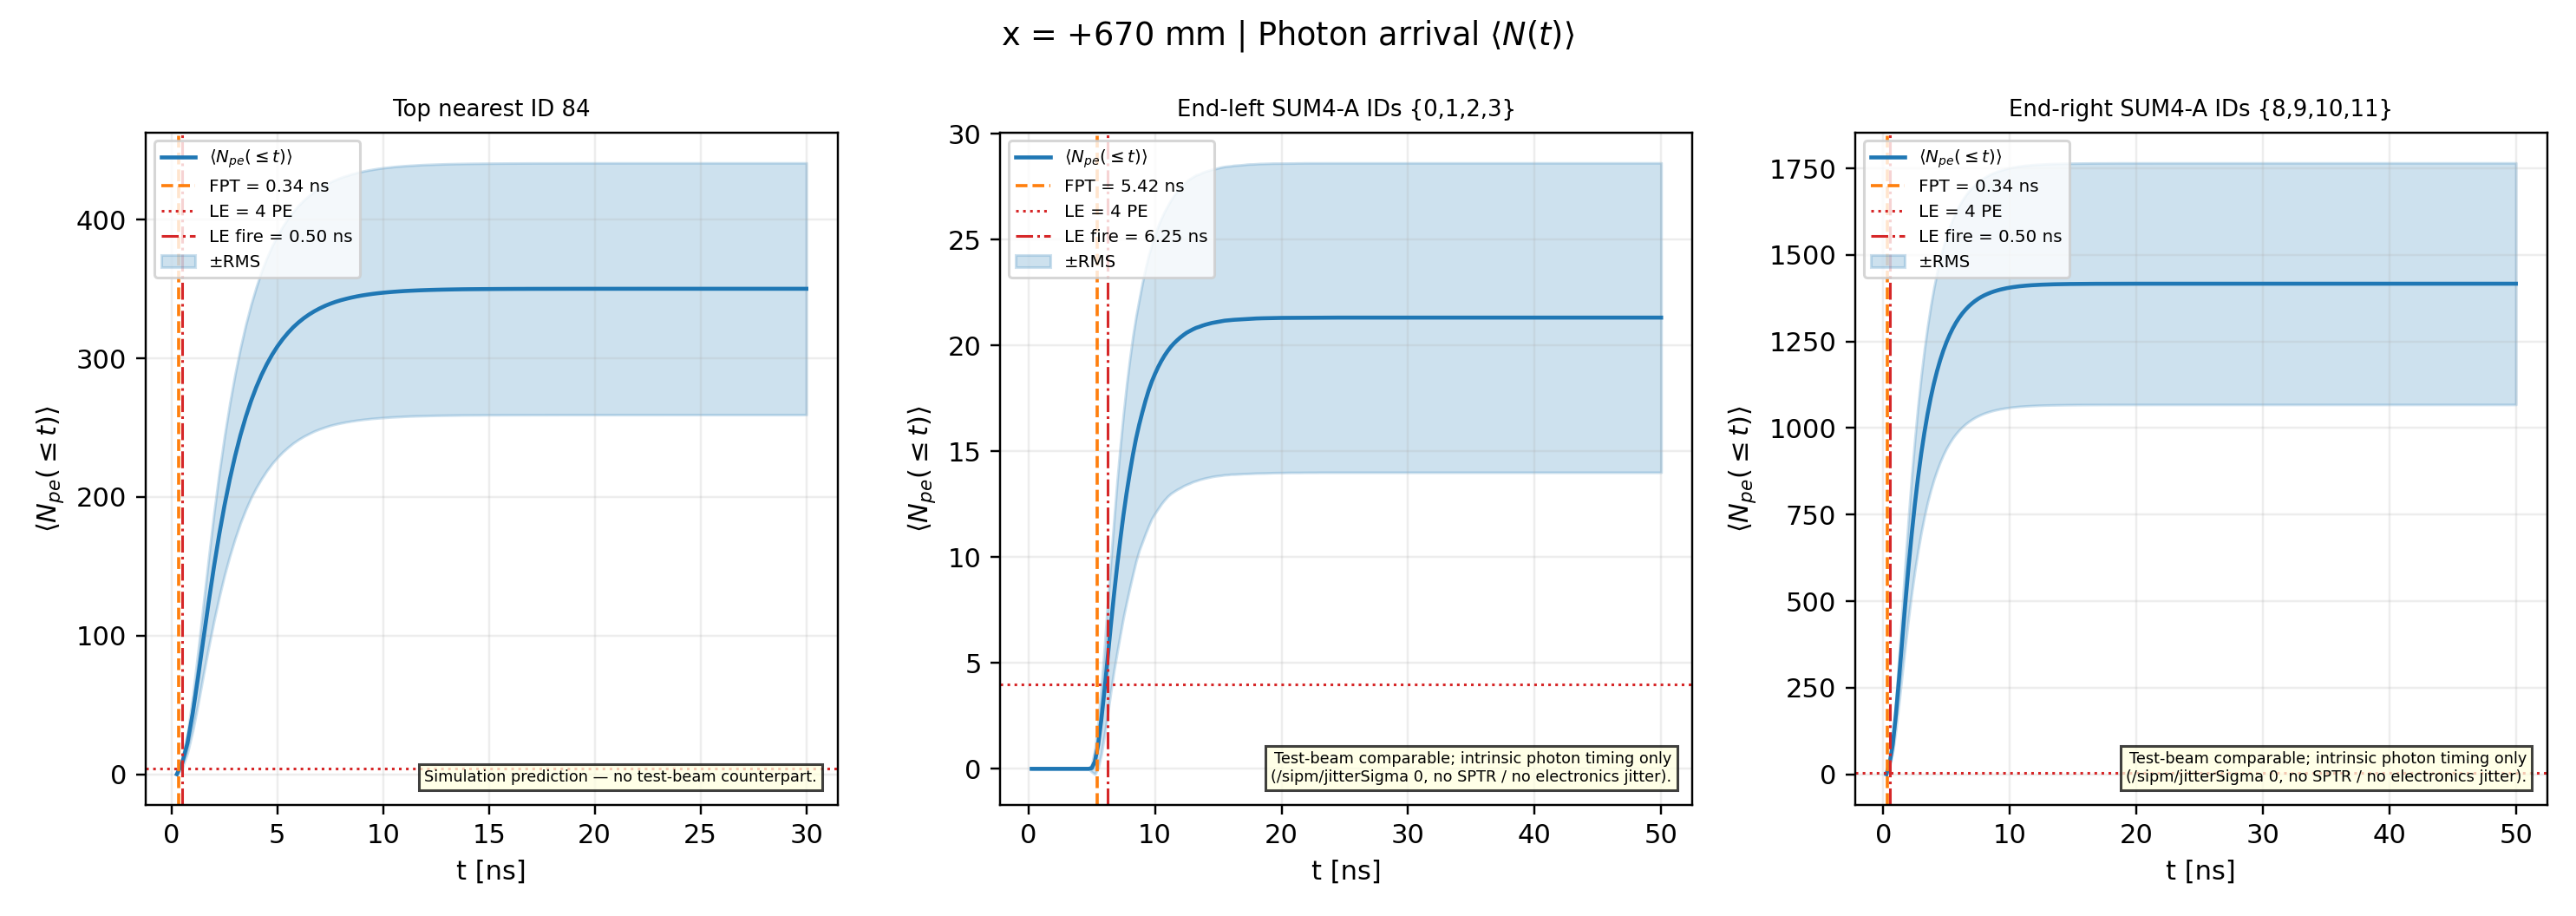
\includegraphics[width=\textwidth,height=0.78\textheight,keepaspectratio]{figs/exec11_arrival_670mm.png}
\end{frame}
\begin{frame}{Position x=690 mm}

\begin{columns}[T]
  \column{0.52\textwidth}
  
\includegraphics[width=\textwidth]{figs/muon_690mm_geometry.png}
  \column{0.46\textwidth}
  
\includegraphics[width=\textwidth]{figs/muon_690mm_top_profile.png}
  \tiny
  \begin{tabular}{lr}
    \toprule Quantity & Value \\ \midrule
    End L $N_{pe}$ & $41.4\pm0.3$ \\
    End R $N_{pe}$ & $3383.2\pm18.3$ \\
    Nearest Top ID & 85 (window-track exception) \\
    Nearest Top $N_{pe}$ & $353.0\pm2.0$ \\
    Nearest Top $\langle t\rangle$ &
      $2.7881\pm0.0023$ ns \\
    Nearest Top FPT & $0.34236\pm0.00019$ ns \\
    \bottomrule
  \end{tabular}
\end{columns}

\end{frame}
\begin{frame}{Run 31 $|$ x = +690 mm $|$ Photon arrival $\langle N(t)\rangle$}
\centering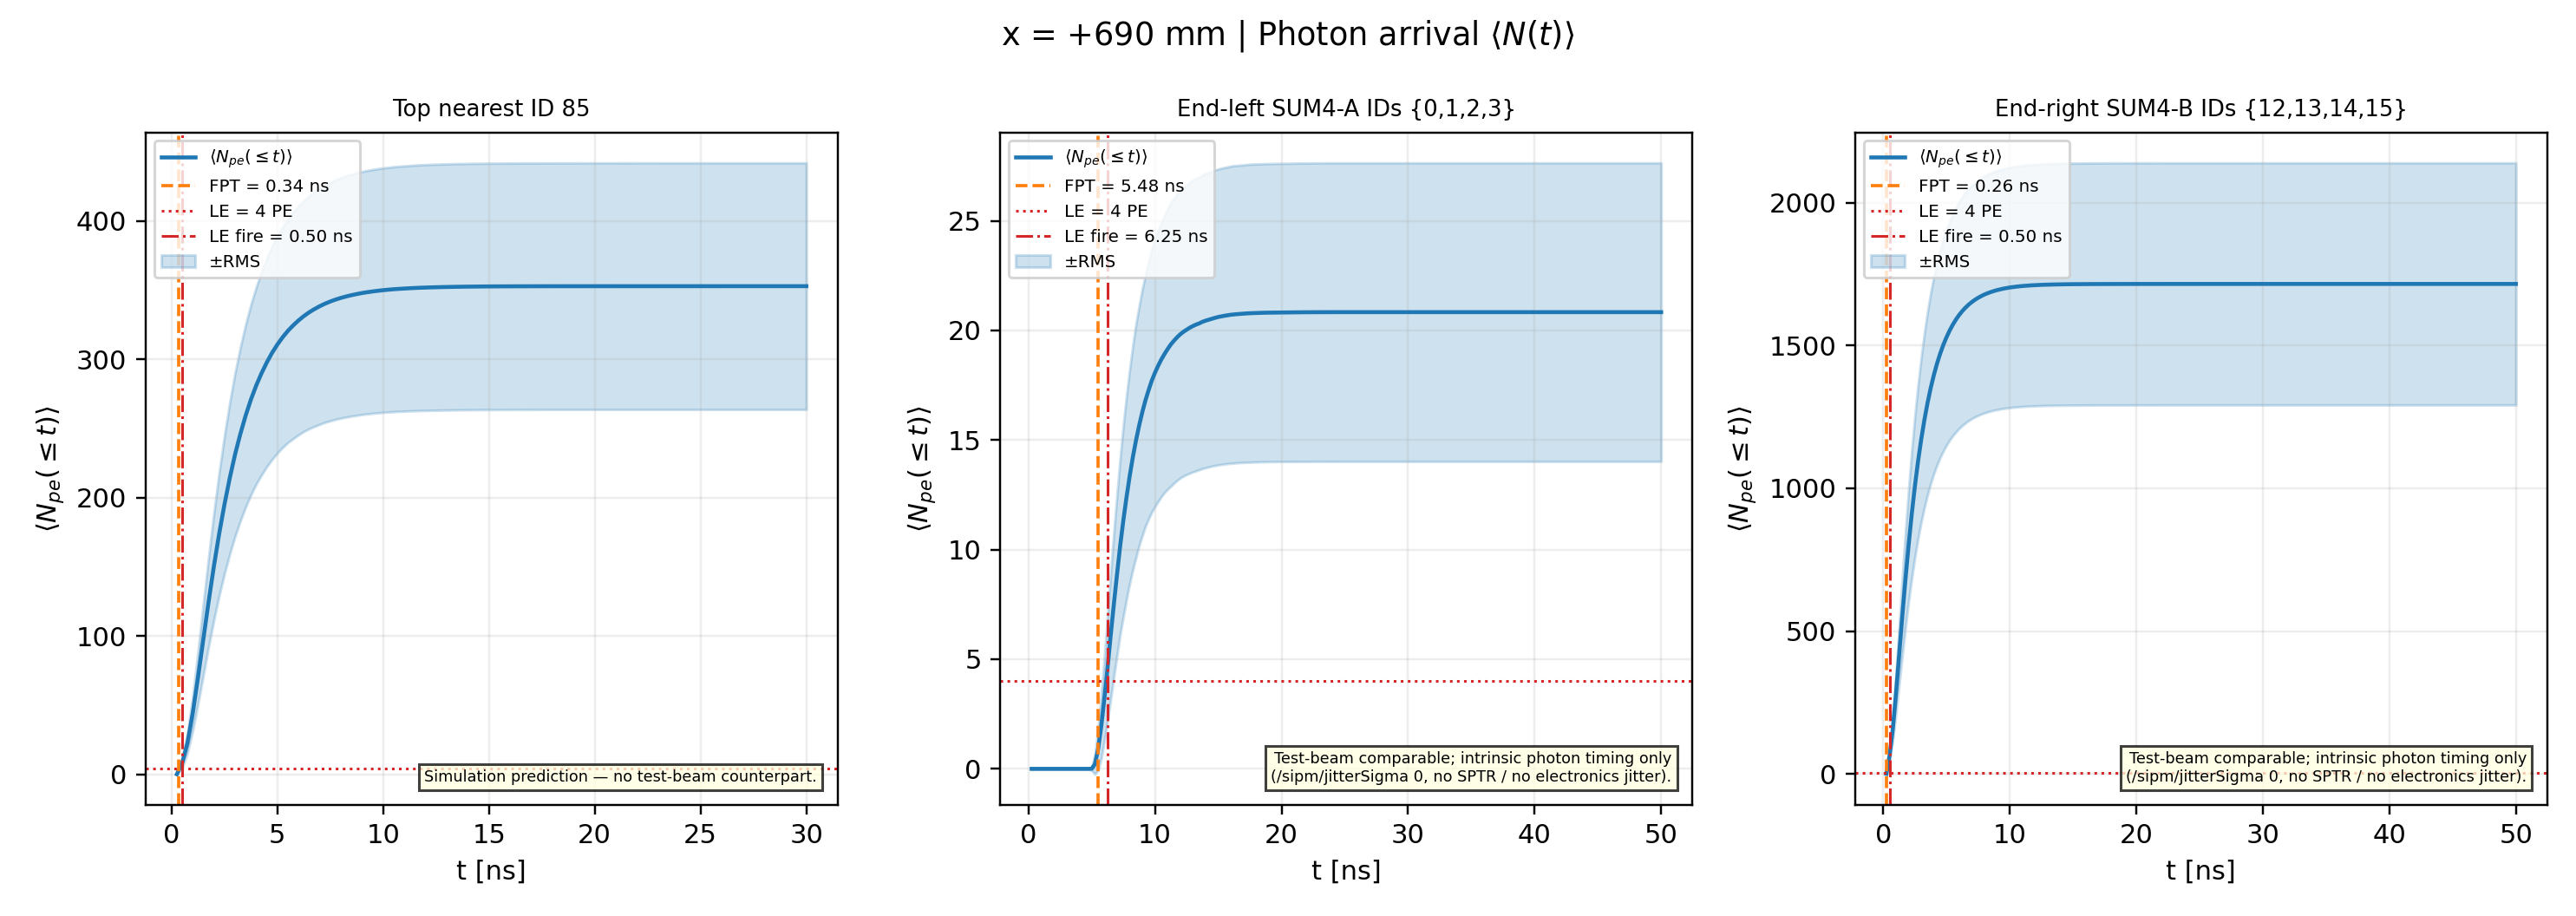
\includegraphics[width=\textwidth,height=0.78\textheight,keepaspectratio]{figs/exec11_arrival_690mm.png}
\end{frame}
\appendix
\begin{frame}{Backup: validation and gates}

\begin{itemize}
 \item 31/31 ROOT files pass: event IDs 0--1999, matching beam x, aggregate IDs 0--85.
 \item Top localization passes all positions: strict nearest maximum except the documented
       $x\equiv10\pmod{20}$ window-track effect (maximum among nearest two, deficit below 15\%).
 \item At x=300 mm the two candidates differ by only 0.08 sigma and pass as a statistical tie.
 \item MPT checks pass: RINDEX 1.58, yield 10400/MeV, decay 1.8 ns, rise 0.7 ns,
       ABSLENGTH 160 cm, emission peak 408.8 nm.
\end{itemize}

\end{frame}
\begin{frame}{Backup: ID18 impact maps}
\centering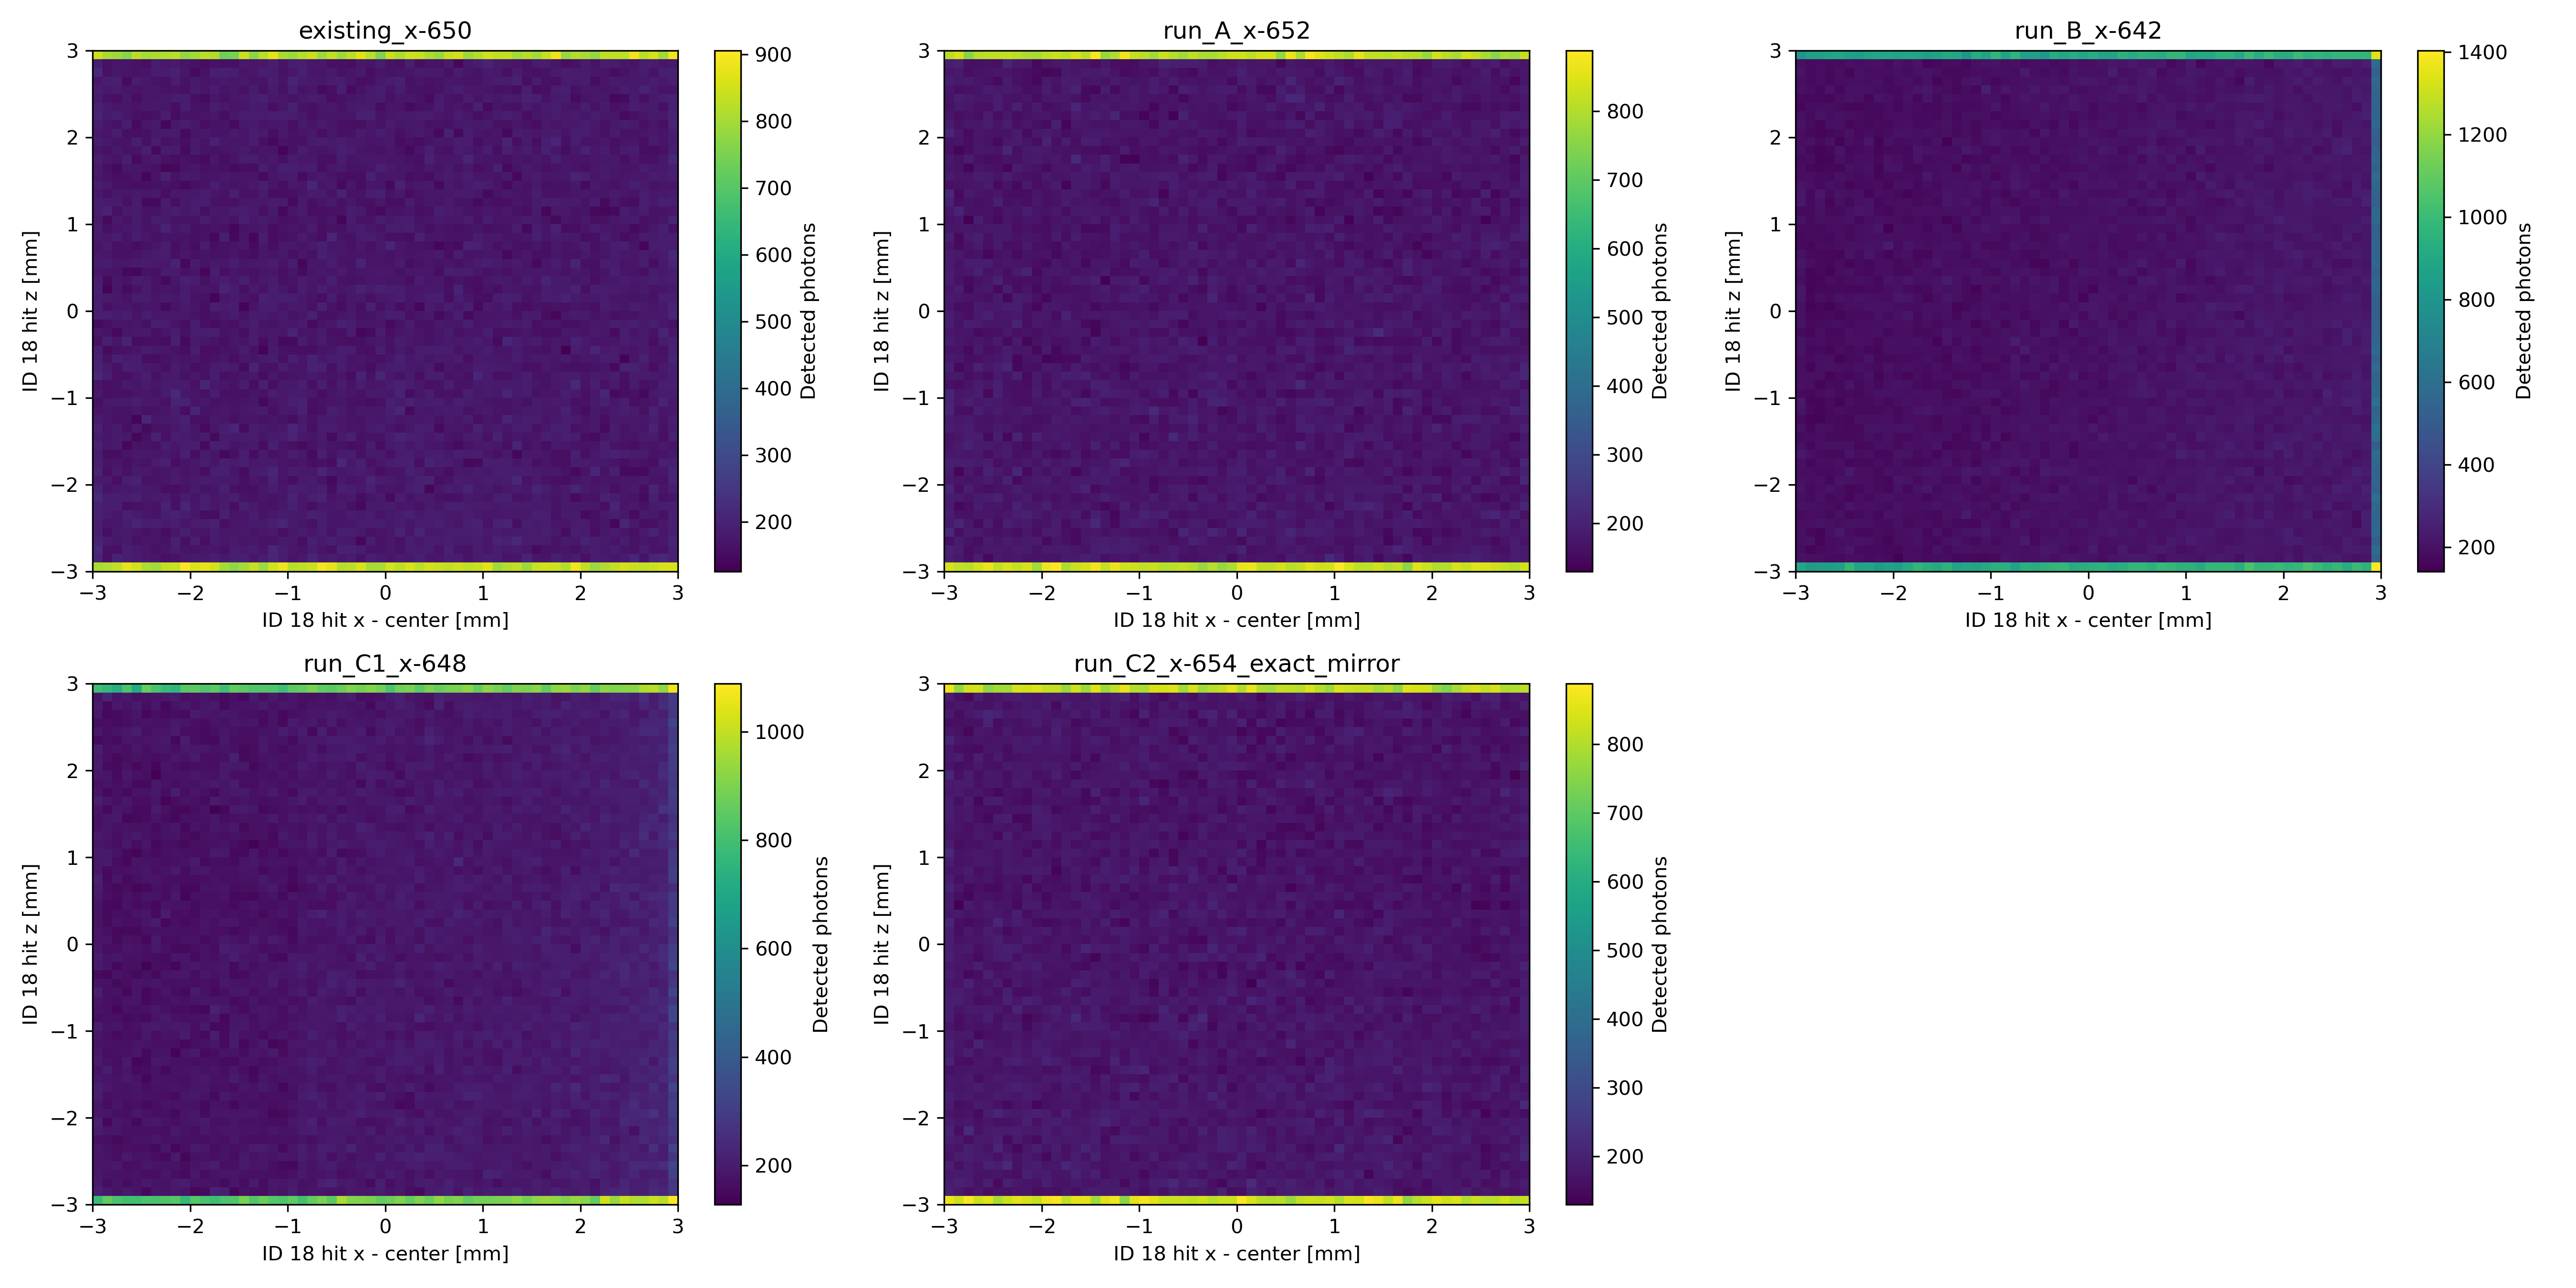
\includegraphics[width=\textwidth,height=0.78\textheight,keepaspectratio]{figs/exec08b_id18_impact_maps.png}
\end{frame}
\begin{frame}{Backup: why a 4-PE leading-edge threshold}

\begin{enumerate}\small
 \item \textbf{Noise rejection at hardware parity:} 1 PE is dark-count territory;
       2--3 PE is reachable by correlated crosstalk in the real SiPM.
       4 PE is the lowest fixed threshold outside the correlated-noise spectrum,
       matching the operating point of a hardware leading-edge discriminator.
 \item \textbf{Slope optimum:} $\sigma_t\approx\sigma_V/(dV/dt)$; with the
       0.5/5 ns SPE the SUM4 pulse has maximal rising-edge slope in the first
       few PE. Lower thresholds expose the high relative variance of first-photon
       order statistics; higher thresholds reduce slope and increase walk.
 \item \textbf{Far-end efficiency:} minimum signal in the scan is End~R
       $\langle N_{pe}\rangle=41.1\pm0.3$ at $x=-690$ mm;
       4 PE ($\approx10\%$ of the minimum pulse) keeps trigger efficiency
       $\approx100\%$ at all 31 positions, avoiding position-dependent selection bias.
 \item \textbf{Bounded, correctable walk:} fixed-threshold time-walk is small
       compared to $\sigma_{group}$ at 4 PE and is parametrized for future
       correction via \texttt{HOOK\_WALK} (no correction applied in any campaign).
\end{enumerate}

\end{frame}
\begin{frame}{Backup: timing methodology}

\begin{itemize}
 \item SUM4 groups: \{0..3\}, \{4..7\}, \{8..11\}, \{12..15\}.
 \item Single-PE response: normalized 0.5/5 ns double exponential.
 \item Absolute leading-edge threshold: 4 PE equivalent
       (noise rejection, slope optimum, $\approx100\%$ efficiency at all 31 positions;
       see dedicated backup slide for full rationale).
 \item Estimator: $\sigma(\Delta T_{AB})/\sqrt{2}$.
 \item \texttt{HOOK\_WALK}: pending; no time-walk correction exists or was invented.
 \item EXEC\_09 anti-artifact audit verifies common threshold, pulse, t=0 and estimator.
\end{itemize}

\end{frame}
\begin{frame}{Backup: glossary}

\scriptsize\begin{description}
 \item[HOOK\_WALK] Reserved insertion point for future leading-edge time-walk correction.
 Fixed 4-PE threshold means larger pulses cross earlier; no correction applied in any campaign
 (\texttt{congruent\_sum4\_timing.C:305--315}).
 \item[FPT] First photon time: first detected photon per event for the stated channel/group.
 \item[Fano factor] $F\equiv\mathrm{Var}(N_{pe})/\langle N_{pe}\rangle$.
 Equals 1 for pure Poisson; grows linearly with $\langle N_{pe}\rangle$ when Landau
 $\Delta E$ fluctuations are present: $F=1+c\langle N_{pe}\rangle$.
 \item[Group A / Group B] Same-End SUM4 groups: A=\{0--3\}, B=\{4--7\} on End~L;
 mirrors \{8--11\}, \{12--15\} on End~R.
 $\sigma_{\rm group}=\sigma(\Delta T_{AB})/\sqrt{2}$
 (\texttt{congruent\_sum4\_timing.C:218--221}).
 \item[Intrinsic sigma] Excludes SPTR and electronics jitter; 88 ps hardware value not directly comparable.
 \item[Moyal] Closed-form analytic approximation to the Landau density, used for
 stable MINUIT fits. Undershoots the extreme Landau right tail.
 \item[SPTR] Single Photon Time Resolution: SiPM intrinsic single-PE jitter.
 Excluded from all EXEC\_12 results (jitter$=0$); re-introduced via EXEC\_02b hooks,
 summed in quadrature with electronics jitter.
 \item[SUM4] Analog sum of four SiPMs: \{0--3\}, \{4--7\}, \{8--11\}, \{12--15\}
 (\texttt{congruent\_sum4\_timing.C:218--221}).
 \item[Timing gate] The comparison script \texttt{exec08b\_timing\_gate.py} tests whether
 EndTop $\sigma_{\rm group}$ is smaller than End-only $\sigma_{\rm group}$ at $x=0,\pm400$ mm.
 It applies no time acceptance window on individual photon arrivals; all ROOT TTree photons are used.
 \item[Window-track collection effect] Local ($\pm2$ mm) increase of first-pass solid angle when a
 track passes offset from a Top window centre. Empirically $\approx9.8$\% at $\approx12\,\sigma$
 (five-run test); null at centre and midpoint; symmetric. Geometric working hypothesis.
 \item[$t_N$ / time-to-threshold] Arrival time of the $N$-th detected photoelectron per event
 in a given group. $\sigma(t_N)$ is the single-side photon-counting timing resolution at
 an ideal $N$-PE digital threshold. Excludes SPE pulse convolution jitter present in $\sigma_{\rm group}$.
 \item[(exact geometry)] Nearest SiPM agrees with maximum, or covered by window-track exception.
 x=300 mm is a statistical tie.
\end{description}

\end{frame}
\begin{frame}{Backup: EndTop versus End-only tail audit}
\centering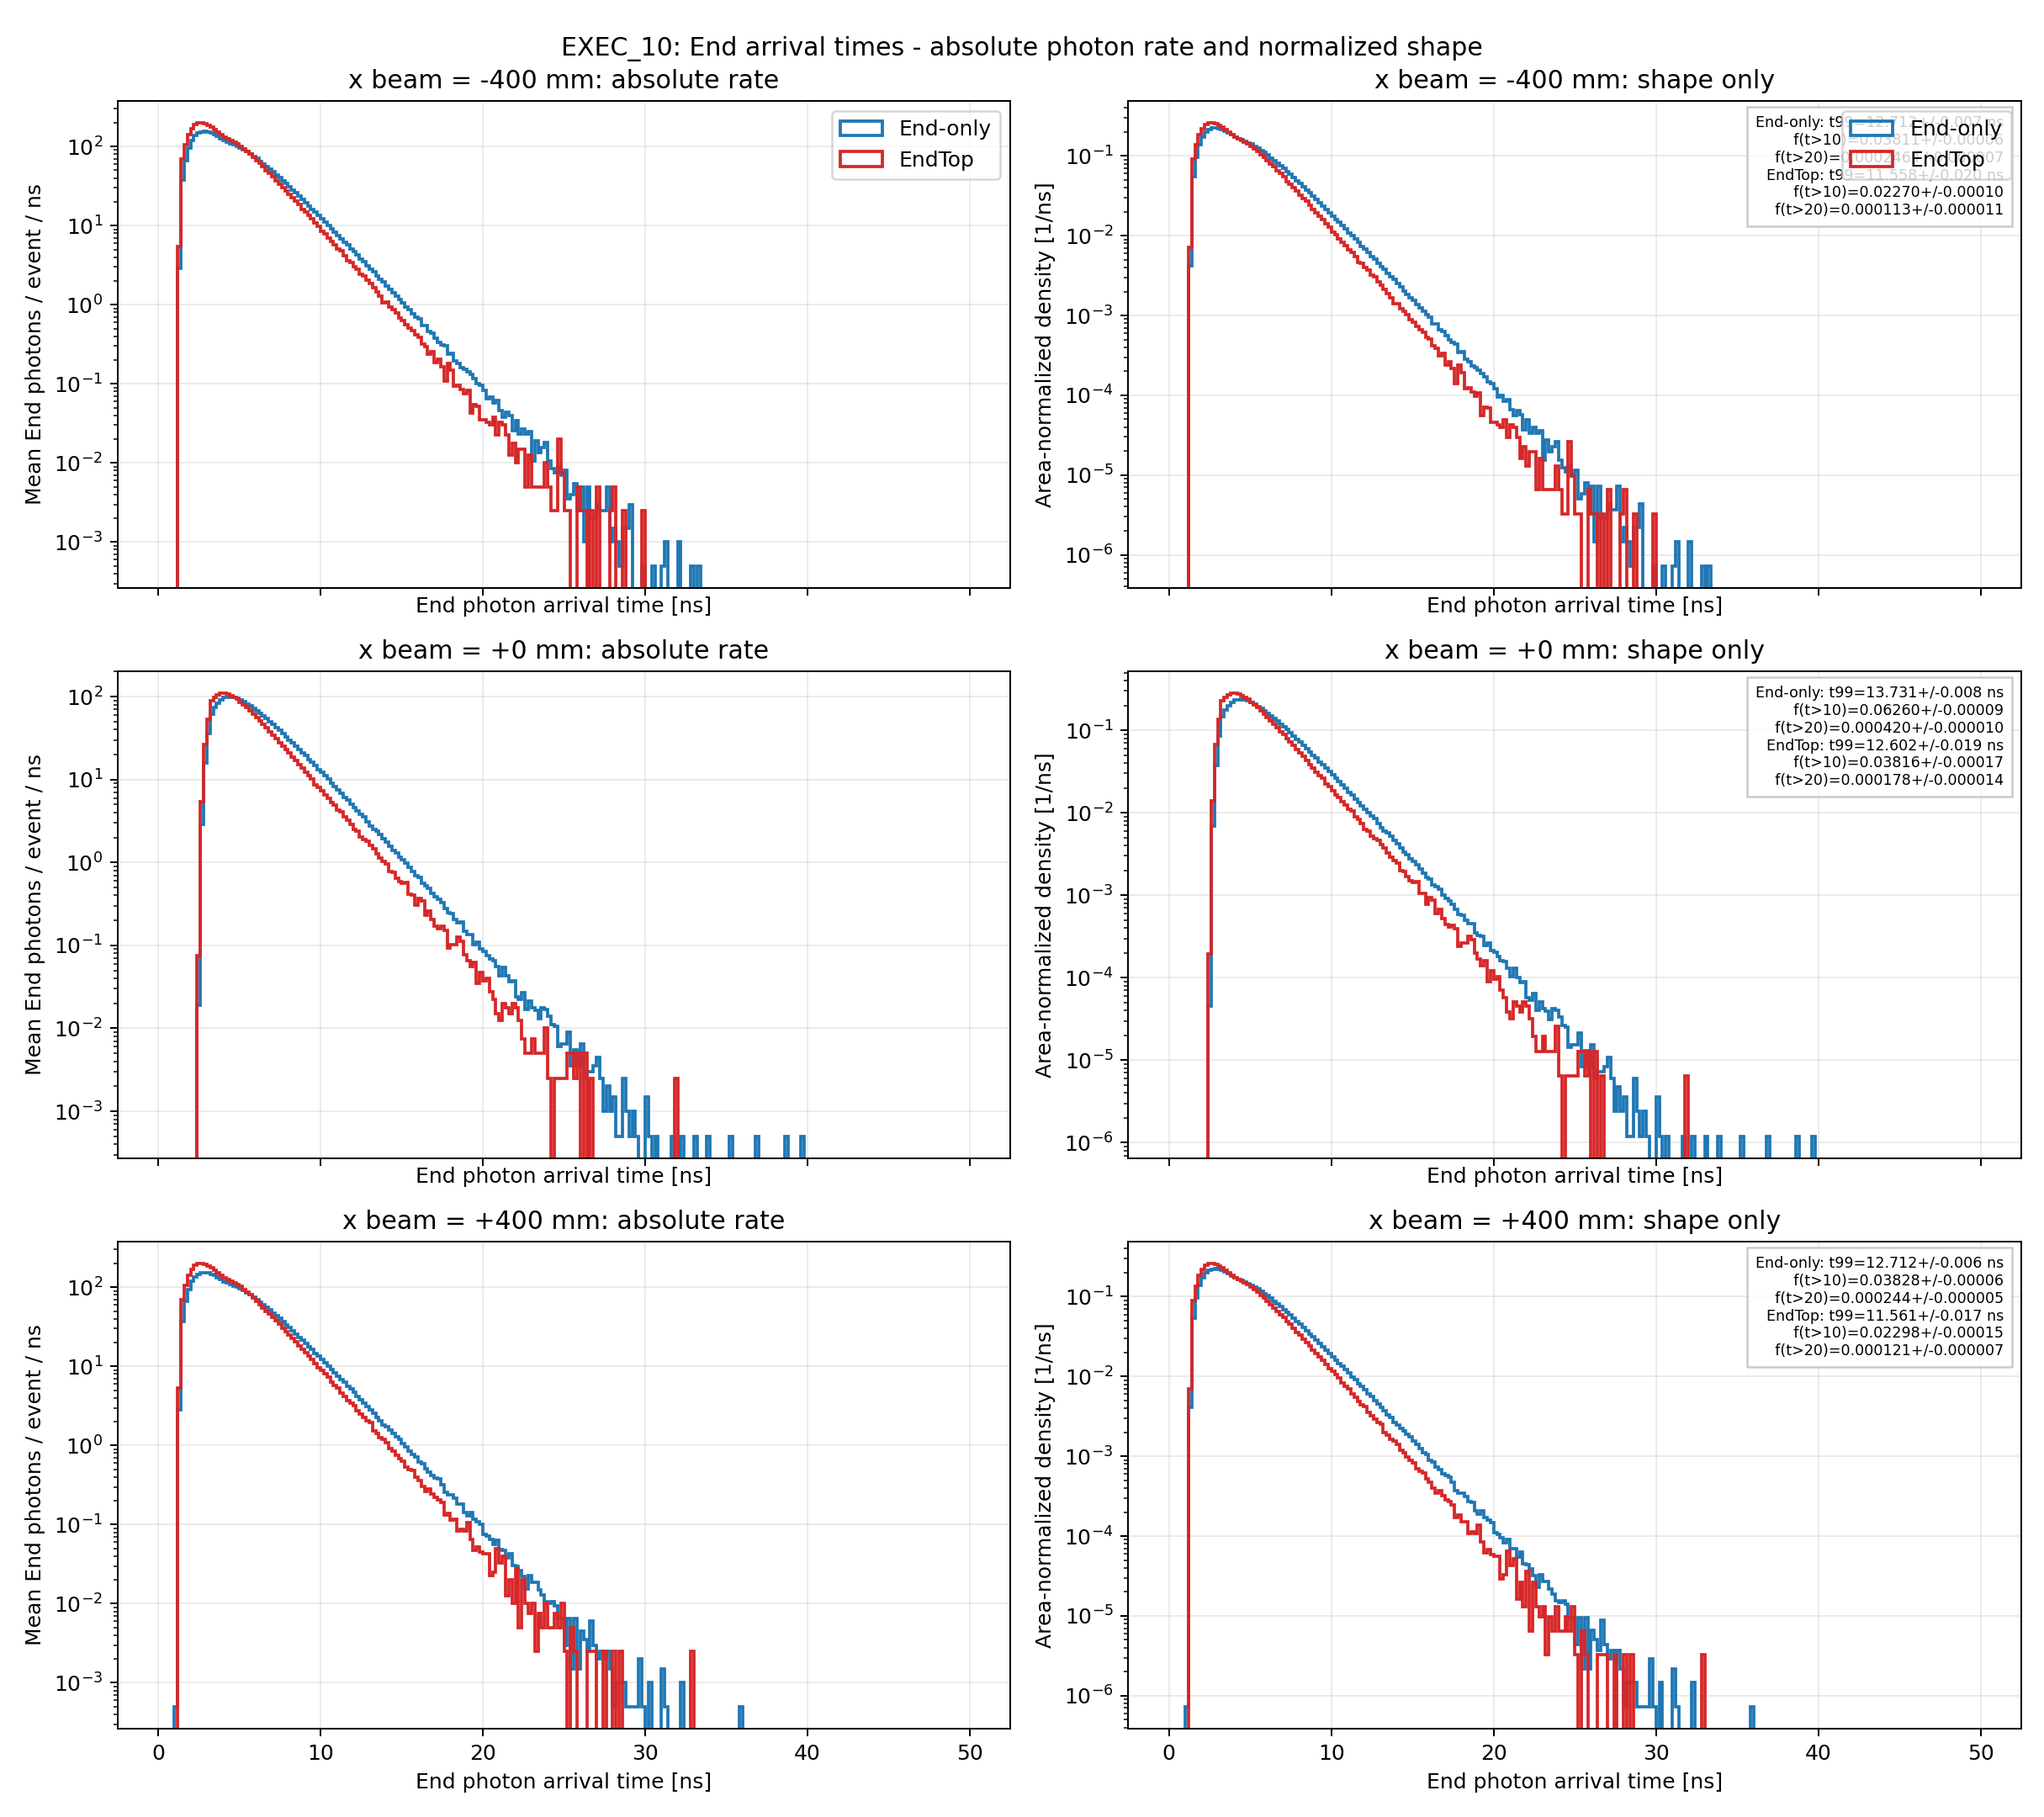
\includegraphics[width=\textwidth,height=0.78\textheight,keepaspectratio]{figs/exec09_tail_comparison.png}
\end{frame}
\end{document}
